\bookpart{任务扩展与可信决策}{Task Extensions and Trustworthy Decisions}
\label{part:rl-task-expansion-and-trustworthiness}

\BookPartGuide{%
一个策略在固定任务中取得较高回报，还不足以说明它能迁移到新任务、与其他行动者协作，或在安全约束下执行。任务改变会影响已有交互记录的适用范围，其他行动者的选择会改变行为后果，风险与安全要求则会改变策略的比较标准。本部分沿这三种扩展，检查可以复用什么、怎样训练与适应，以及哪些证据足以支持执行。

第~\ref{chap:rl-transfer}章“任务泛化与适应”先确定可复用的是表示、策略、价值、模型还是学习规则，再说明这些对象适用于哪些任务。训练任务与评价任务的划分、允许取得的目标任务交互记录、适应预算和参数更新权限共同界定问题；在这些条件下，才能比较直接迁移、基于历史的适应与基于梯度的适应，并诊断迁移退化的原因。

第~\ref{chap:rl-multi-agent}章“多智能体协作和博弈”把单一行动者扩展为多个相互影响的参与者。收益关系决定协作、竞争或混合的行为标准；各自能够读取的观测、历史与消息决定可执行策略。联合交互记录的收集、价值估计与策略更新需要共同处理其他参与者的依赖和变化，集中训练时可取得的状态也不能自动供分散执行使用。

第~\ref{chap:rl-trustworthy}章“可信强化学习”把期望回报之外的风险、模型偏差、安全约束与可靠性要求写成可检验主张。风险敏感目标、鲁棒优化、受约束学习和执行时保护分别改变不同环节，所提供的保证依赖各自的模型、扰动集合、评价协议或安全证书。三章最终都要回到适用任务、比较预算与失效条件：一次测试成功只能支持对应范围的主张，条件改变后需要重新评价。}


% Outline: 6
\chapter{任务泛化与适应}
\label{chap:rl-transfer}

前几章始终在“同一个任务”里学习：地图、终点、移动规律和奖励一旦定下，训练和部署面对的都是它。但现实中的任务很少一成不变。设想一辆小车已经学会绕过障碍：若终点换到地图另一侧，它仍然知道各方向怎样移动，只需重新选择路线；若地图不变而地面变滑，原来那条路线的到达概率就可能改变。两种变化都在问“旧知识能不能用于新任务”，可需要保留的东西和需要重新估计的东西截然不同。这就是本章的主题——任务泛化与适应：把在一批任务上学到的知识，用到没见过或已经变化的新任务上。除了“什么变了”，还有两个同样关键的问题：小车是否被告知新终点或地面参数？是否允许它通过试探弄清这些？共享的物理规律、取得的目标描述或任务交互记录、以及获准学习的权限，是三个互不替代的条件。

第~\ref{chap:rl-learning}~章已经说明怎样在单个任务中学习价值、策略与环境模型。现在把这些学习对象放到多个任务之间考察：声明哪些要素允许变化后，才能判断某个预测或行为规则是否仍有原来的含义；声明可读取的任务描述、观测和交互预算后，才能确定新任务中的策略如何形成。训练负责获得可复用知识，部署负责调用或调整这些知识，验证则检查所声明的任务范围内是否确有收益。图~\ref{fig:rl-transfer-map}~中的反馈箭头表示，失败有时要求重查共享假设，而不只是延长训练。历史能否保留会影响动作选择的观测、动作与奖励记录、固定日志能否支持新行为，分别沿用第~\ref{chap:rl-information}~章的信念与覆盖条件；反馈究竟评价什么，仍由第~\ref{chap:rl-reward}~章的目标规定。

\begin{figure*}[t]
  \centering
  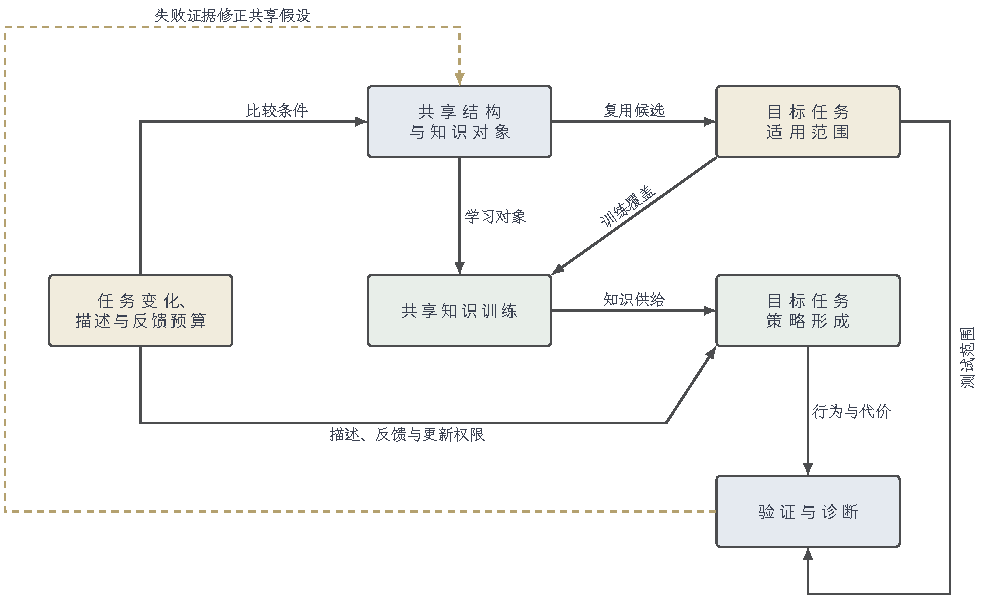
\includegraphics[width=166.345mm]{figures/10-reinforcement-learning/03-task-expansion-and-trustworthiness/tikz/rl-transfer-map.pdf}
  \caption{任务泛化与适应的论证关系。实线标明条件约束或知识供给，虚线表示验证后的修订反馈；不是所有方法都必须顺序执行的流程。部署中的记忆、参数更新和持续交互可以组合。图为本章关系的原创示意。}
  \label{fig:rl-transfer-map}
\end{figure*}

% Outline: 6.1
\section{任务泛化与适应问题}
\label{sec:rl-transfer-problem}

% Outline: 6.1.1
\subsection{任务要素的变化范围}
\label{sec:rl-transfer-components}

沿用前文宽4、高3、障碍位于$(2,2)$的导航地图，起点仍为$(1,1)$。基准任务以$(4,3)$为终点，合法意图方向以$0.8$概率执行，两侧各以$0.1$概率滑移；进入终点得1，其他非终止步得$-0.04$，吸收后奖励为0，折扣为$\gamma=0.9$。这些是统一的教学设定，不是实验测量结果。我们分别改变终点、移动噪声、观测符号或动作编码，观察旧策略会在哪一步失去依据：终点决定去哪里，移动规律决定动作会到哪里，观测符号决定怎样解释当前收到的观测，动作编码决定命令的物理含义。为把这些变化放在同一套记号下比较，用$c$标识一项任务，并把所有允许的任务组成任务族。

\begin{definition}[任务族]
  \label{def:rl-transfer-family}
  给定非空任务参数集合$\mathcal C$和共同折扣$0\leq\gamma<1$。对每个$c\in\mathcal C$，状态空间$S_c$、行动空间$\mathsf A_c$和观测空间$\mathsf O_c$均配可测结构，每个状态有非空合法动作集$\mathsf A_c(s)$。初态分布$\mu_{0,c}$是$S_c$上的概率测度，$T_c$是从合法状态—动作对到$S_c$上概率测度的转移核，$K_{o,c}$是按声明时序产生观测的概率核，$R_c(s,a)$是可积逐步奖励在状态动作给定后的条件均值。
  用$c$索引任务模型
  \[
    \mathcal M_c=(S_c,\mathsf A_c,T_c,R_c,K_{o,c},\mu_{0,c},\gamma).
  \]
  其中动态环境部分记为$\mathcal E_c=(S_c,\Sigma_{S_c},\mathsf A_c,\Sigma_{A_c},\mu_{0,c},T_c)$。任务族由动态环境、奖励与终止反馈机制、观测机制，以及执行前提供的任务描述和可记录字段共同确定。比较时须声明哪些分量随$c$改变，哪些共同固定；有终止事件或有限时域时，还须规定终止机制与时域。
\end{definition}

同一状态集合上的两个奖励函数已经定义了不同任务；状态和动作的维数相同，并不要求转移、奖励或语义相同。若要根据随机奖励和终止反馈辨识任务，还须给出这些反馈与后继状态的联合条件分布：均值$R_c$本身不能确定反馈似然。表~\ref{tab:rl-transfer-changes}~列出四种单因素变体，其中执行前可读的描述或参数由实验协议提供，不是把智能体训练中读取过的任务标签或参数一概当作已知。

\begin{table*}[t]
  \centering\small
  \begin{tabularx}{\linewidth}{@{}>{\raggedright\arraybackslash}p{23mm}*{3}{>{\raggedright\arraybackslash}X}@{}}
    \toprule
    变化分量 & 保持不变的对象 & 执行前可读的描述或参数 & 需要重算或重新学习的对象\\
    \midrule
    终点与奖励 & 地图、物理移动规律 & 可能提供目标坐标；也可能只有到达反馈 & 新目标价值、路线选择；终止规则改变时还包括有效转移\\
    移动噪声 & 目标含义、地图、命令语义 & 位置与移动结果；风参数未必给出 & 转移概率、长期后果、控制策略\\
    观测符号 & 潜在地图与物理动作 & 新符号图像；对应表可能未知 & 感知对齐，必要时重学历史表示\\
    左右命令互换 & 物理空间、目标、观测 & 命令标签与执行结果 & 动作映射、合法命令集与技能接口\\
    \bottomrule
  \end{tabularx}
  \caption{同一导航地图中的任务变化。每行单独改变一个因素，数字与任务均为教学构造。更换吸收终点会改变完整MDP的转移核，不能只因物理移动规则相同就声称共同动力学。}
  \label{tab:rl-transfer-changes}
\end{table*}

表中的终点变化还需要检查吸收约定。如果进入终点后不能继续移动，换终点就同时改变了转移核，不能只归为奖励变化。要单独检验奖励能否复用，我们改用共同终止规则：所有任务在相同时间结束，或保持固定吸收出口而只改变沿途地标的奖励。有限时域的前一种设定还须把剩余时间纳入状态，才能用同一个转移核描述到时终止。这些独立变体用于隔离复用条件，不是基准网格的另一组求解结果。

还要区分两个时间尺度。在一次适应试验中，未知风向可以固定不变，只是智能体逐渐认识它；也可以每个回合都改变。前者的证据指向同一估计对象，后者的旧证据可能已经过时。固定任务辨识在第~\ref{sec:rl-transfer-identification}~节展开，变化任务的跟踪在第~\ref{sec:rl-transfer-tracking}~节另行定义。

% Outline: 6.1.2
\subsection{目标任务信息的可用条件}
\label{sec:rl-transfer-information}

同样是换终点，地图直接标出坐标时，小车可以据此规划；只有抵达才发奖励时，它需要从经历中排除候选位置。若隐藏的是风向，即使终点已知，也可能要试一次移动才能区分转移规律。前一小节比较任务中什么发生了变化，这里固定这些变化，转而检查智能体能看见什么。已知目标只能消除目标身份的不确定性，不能同时消除动力学的不确定性。

执行前提供的目标坐标、参数或语言指令称为\term{显式任务描述}（explicit task description）：它直接告诉智能体任务的某些条件。描述未给出的条件，可以从已记录的观测、动作、奖励与终止标记中推断，下文将这组按时间保存的记录称为\term{任务交互记录}（task interaction records）。若现有记录不足以区分候选任务，还可以选择会产生不同反馈的动作；这种\term{主动辨识}（active identification）通过行动取得能区分候选任务的新观测或奖励，不是对同一份历史多计算几遍。语言指令也需要与奖励和控制接口有可信的对应关系，单独一句话并没有给出完整MDP。

设训练任务用编号1和2分别代表东、西两个终点。把编号交换、保留所有轨迹的物理内容，再相应交换训练标签，并不会改变问题难度。对于从未出现的编号3，训练记录没有告诉模型它是北端终点还是强风任务。编号能索引记住的任务，却没有坐标那样的几何语义。新编号上的零样本迁移必须另有描述映射，不能依靠编号的大小顺序。

任务编号不自带物理含义，历史编码器的输出$\bm z_t$也不自带概率含义。奖励预测或策略损失可以使这个向量保留与任务有关的线索，但没有保证它的分量构成归一化、校准的任务后验。还要先检查历史本身是否有区分力：若两个任务在所有获准动作下都产生相同的可见反馈分布，增加历史长度或模型容量也无法区分它们。第~\ref{sec:rl-transfer-belief}~节据此分别考察记录本身不能区分任务和推断器未利用已有区分线索的情形。

% Outline: 6.1.3
\subsection{零样本、少样本与持续适应预算}
\label{sec:rl-transfer-budget}

一个网络保持权重不变，却可能在历史窗口中读过大量目标任务反馈；另一个网络在固定日志上更新参数，却没有增加真实交互的权限。只报告是否更新网络，无法判断两者各用了多少目标任务观测、奖励与终止反馈。比较预算时，需要同时记录可读取的任务描述、观测及交互记录，会变化的记忆或参数，以及推断和更新所需的计算。

本章将\term{零样本执行}（zero-shot execution）限定为不使用目标任务反馈进行额外学习、记忆适应或模型选择的执行。它仍可读取给定任务描述和正常控制所需的观测。部分可观测任务中的状态滤波应预先声明：在已给定任务模型下估计当前位置，属于控制所需的状态估计；利用偏移反馈推断未知风向，则更新了对未知任务参数的判断，属于适应，即使只发生在一个回合内、网络权重始终不变。\term{少样本适应}（few-shot adaptation）使用预定数量的目标经验形成策略；经验可以来自给定日志，也可以来自获准交互。\term{持续适应}（continual adaptation）允许在部署过程中反复更新任务参数估计、潜变量记忆或策略，评价必须计入这一过程中的表现。

文献中的zero-shot可能采用不同口径，例如仅要求测试时不更新网络权重。比较论文结果时，应继续核对实际读取了哪些目标任务反馈、是否保留任务特定记忆、是否据此选择模型，再按本章预算分类；论文名称本身不能代替这些协议。

表~\ref{tab:rl-transfer-budget}~用教学协议固定这些差别。$B$表示适应交互步数，$L$表示最多保留的历史长度，$K$表示梯度步数；实际论文还应报告各回合长度，不能仅以“若干回合”比较不同任务。

\begin{table*}[t]
  \centering\small
  \begin{tabularx}{\linewidth}{@{}>{\raggedright\arraybackslash}p{19mm}*{6}{>{\raggedright\arraybackslash}X}@{}}
    \toprule
    协议 & 目标交互 & 可见反馈 & 上下文 & 参数更新 & 额外计算 & 选模查询\\
    \midrule
    零样本 & 无适应步；执行另计 & 描述、执行观测 & 不累计用于辨识未知任务的反馈 & 0 & 固定推理预算 & 0\\
    固定日志适应 & 新交互0 & 日志给定字段 & 至多$L$步 & 至多$K$步 & 推断与反传均计 & 预先固定\\
    少量在线适应 & 总计$B$步 & 约定奖励及终止 & 至多$L$步 & 至多$K$步 & 探测、规划均计 & 纳入$B$\\
    持续在线适应 & 全程累计 & 按到达时刻可见 & 记忆重置规则固定 & 频率与总量均报 & 每步和累计成本 & 不用未来成绩选模\\
    \bottomrule
  \end{tabularx}
  \caption{目标任务预算的不同分量。各列共同定义协议；“固定日志”与“固定参数”不是同义词。本表为评价口径，不是任何算法的实测回报。}
  \label{tab:rl-transfer-budget}
\end{table*}

假设每回合恰有20步，共运行10回合，这是教学预算而非实测配置。只报告第1回合、按固定控制规则响应观测且不辨识任务或更新策略，回答的是初始执行能力；允许在10回合内学习并报告全部200步回报，回答的是学习期间能否付得起试错成本；先适应10回合，再停止任务学习、另测5回合，回答的是200步适应后的控制能力，但总交互已是300步。三种分数即使相等，也没有相同含义。

初始执行只按预定规则控制和恢复，不包含用于学习任务的探测或选模；允许适应的两种评价，则还要计入这些操作的成本。试探风向和从失败位置返回消耗交互步，选择“最好的第7次更新”则需要查询目标任务成绩。只有把协议允许的这些成本计入，才能比较相同反馈量或计算上限下谁较早达到预先规定的回报，而不是只比较最终执行了多少步。

% Outline: 6.2
\section{可复用决策知识的确定}
\label{sec:rl-transfer-knowledge}

% Outline: 6.2.1
\subsection{由任务要素异同判断共享结构}
\label{sec:rl-transfer-sharing}

有了任务变化、可读取的描述与交互记录、适应预算这三个比较依据，现在可以回到核心问题：哪些旧知识在新任务里仍然“有意义”？看两个对比鲜明的例子。在共同终止规则下只换导航目标，旧的转移模型仍能正确预测“向右会到哪里”；可一旦把左右命令互换，原策略发出的“右”却会执行成向左。两种新任务的观测编码与动作命令都可以沿用相同的张量形状，但只有前者保留了原命令的控制含义。可见“接口长得一样”并不代表“含义一样”。图~\ref{fig:rl-transfer-components}~逐项标出哪些任务分量不变，作为选择复用对象的依据。

\begin{figure*}[htbp]
  \centering
  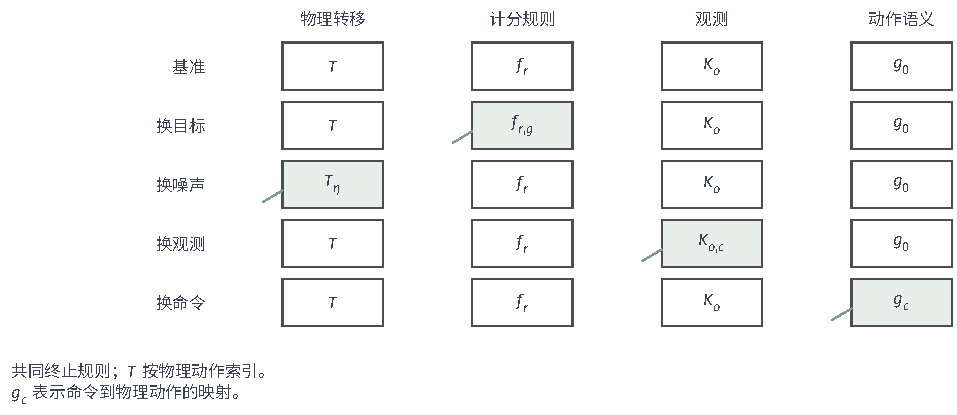
\includegraphics[width=161.988mm]{figures/10-reinforcement-learning/03-task-expansion-and-trustworthiness/tikz/rl-transfer-components.pdf}
  \caption{导航任务族的要素矩阵。相同符号与底纹表示同一分量，斜线及新符号表示变化；“换目标”行使用共同终止规则。$f_r(s,a,s')$表示给定转移后的计分规则，换目标时改为$f_{r,g}$；换噪声保留$f_r$，却可能改变均值奖励$R_c(s,a)$。$T$按物理动作索引，$g_c$把任务$c$的命令映为物理动作，基准接口记为$g_0$；若按命令标签索引，转移核也须相应变换。矩阵为控制变量设计，不表示已由交互记录证实共享关系。}
  \label{fig:rl-transfer-components}
\end{figure*}

图中不变的分量对应一项\term{共享结构}（shared structure）假设，即明确哪些任务对象具有可共同使用的关系。例如，统一状态动作语义后可以要求$T_c=T$；也可以要求奖励由同一组特征线性组合，观测映射到不混淆目标任务中不同最优动作的共同状态，或技能具有相同启动集与终止含义。每项假设约束的对象不同，强弱也不同。“任务相似”不能代替这些可检查的关系。

实验者编写的任务生成器可以保证某个模块不变，此时结构是已知的。若从训练任务的交互记录估计共同转移，再用未参与拟合的留出评价样本检验，则结构是估计结果，带有覆盖与误差条件。仅因两条学习曲线相似而猜测可以共享，只是待检验假设。控制变量比较应在相同状态、相同物理动作及相同反馈定义上检查差别；否则观测编码错误可能被误诊为动力学变化。

相似特征与相似回报都只能提供线索。一个编码器可能把两个外观相近、却需要相反动作的状态合并；两项任务也可能恰好在当前策略访问的区域一致，而在未访问区域完全不同。共同结构的声明必须带上适用状态动作范围。

% Outline: 6.2.2
\subsection{由共享结构确定可复用知识}
\label{sec:rl-transfer-objects}

即使已经确认两项任务的物理移动规律相同，也不能把所有旧参数一股脑儿保留。原因在于不同的学习对象依赖的条件不同：转移模型只预测“给定状态动作后会怎样变化”，只要完整转移与接口不变，它就可能继续适用；价值函数则在此之上还按奖励给这些变化打了分，奖励一变通常就得重算；策略直接选动作，即使动作仍能合法执行，也未必会走向新目标。因此复用要沿每个预测或决策规则的依赖条件逐项判断，而不能按整个网络文件笼统决定“用”还是“不用”。

例如，把终点从$(1,3)$换到$(4,1)$，可保留物理地图与动作效果，但到旧终点的距离和价值不能直接解释新任务。把滑移概率由基准的$0.2$改成教学假设$0.4$，目标坐标仍有相同含义，但旧到达概率必须重新估计。表~\ref{tab:rl-transfer-objects}~将复用对象与所需条件成对列出。

\begin{table*}[t]
  \centering\small
  \begin{tabularx}{\linewidth}{@{}>{\raggedright\arraybackslash}p{21mm}*{3}{>{\raggedright\arraybackslash}X}@{}}
    \toprule
    复用对象 & 共享条件 & 目标任务仍需估计的量 & 典型失效\\
    \midrule
    状态表示 & 保留会改变目标任务动作选择的状态差别；观测可对齐 & 任务特定变量、价值或策略 & 丢掉新目标需要的线索\\
    环境模型 & 相同转移机制或已知模块关系 & 风向、摩擦等特定参数 & 未建模机制改变\\
    奖励特征 & 特征语义不变，新奖励可表示 & 新权重$\bm w_c$ & 新目标不在特征类中\\
    后继表示与特征 & 固定策略、动力学和折扣 & 新奖励权重；必要时补新策略 & 转移变化或策略库覆盖差\\
    价值函数 & 原价值对应目标奖励、转移与策略 & 不满足条件时需重估价值 & 旧数值仍可算但含义已错\\
    策略初始化 & 接口兼容，少量更新有合适方向 & 目标任务参数修正 & 少量目标样本的估计波动导致负适应\\
    技能 & 启动集、可读状态或观测历史、动作效果和终止兼容 & 高层选择、组合或内部适应 & 能启动却不能达到所需效果\\
    \bottomrule
  \end{tabularx}
  \caption{可复用知识及其条件。共享条件说明对象何时有意义，不承诺从有限任务及其交互记录中训练出的模型满足这些条件。来源为本章定义与后文推导的归纳。}
  \label{tab:rl-transfer-objects}
\end{table*}

表中的技能还包含何时交还控制权。它是一段有内部策略和终止条件的持续行为，不是固定长度的动作数组。“绕过障碍”在新任务中可能仍能执行，但若新目标要求中途停在障碍旁，原终止条件就会错过需要的位置。因而要检查启动集、可读状态或观测历史、控制效果和终止条件是否仍服务于新决策，而不只是运行时有没有报错。第~\ref{chap:rl-learning}~章已定义单任务中的时间抽象，这里增加的是这些条件跨任务保持的要求。

% Outline: 6.3
\section{可复用决策知识的适用任务}
\label{sec:rl-transfer-applicability}

选定了复用对象，还必须限定它到底能面对哪些目标任务。同一个旧转移模型，可能适用于只换奖励的任务，却不适用于换了风向的任务；目标条件策略也只有在新目标描述有可解释语义时才能用。下面依次从任务生成关系、奖励变化、动力学变化、观测动作接口变化四个角度检查复用条件；同一个目标任务可能同时涉及其中几项。

% Outline: 6.3.1
\subsection{训练任务与目标任务的生成关系}
\label{sec:rl-transfer-distributions}

从同一目标和风向下多走几次，增加的是该任务的经历；另换目标或风参数，才增加了任务层的变化。要评价多任务训练的平均损失，需要把这两层随机性分别计算。用$p_{\text{训练}}(c)$表示训练任务总体分布，$p_{\text{目标}}(c)$表示声明的部署任务分布。给定$c$及行为策略$\beta$后，理论轨迹$\tau$的分布记为$P_{\mathcal E_c}^\beta$，在当前离散表示或共同支配测度下用$p_c^\beta$表示其质量函数或密度。协议实际取得的是可见记录$Z=b_c(\tau)$，其分布为$P_{\mathrm{rec},c}^\beta$；记录字段包括获准采集的状态或观测、动作、奖励与终止标记。轨迹律由初始分布、转移、观测与奖励和终止反馈的联合规律，以及行为策略共同决定；$R_c$只给出奖励均值，不能代替反馈分布。只拟合$(s,a,s')$时可以边缘化其余字段，但损失或采集策略用到的反馈必须保留。先在同任务内对轨迹取平均，再按训练任务的抽取概率平均：
\[
  \mathbb E_{c\sim p_{\text{训练}}}
  \mathbb E_{\tau\sim p_c^\beta}[\ell(c,\tau)].
\]
内层期望回答某项任务的平均损失，外层期望回答训练总体如何给各任务加权。用可见记录估计这个期望，还要求损失可由$Z$计算，或另有从记录识别损失期望的条件。即使一项任务内有大量轨迹，也没有因此获得其他目标或风向下的证据。

有限任务清单$\{c_1,\ldots,c_n\}$只给出了实际训练对象。任务生成器是可继续采样新对象的程序，其采样规则定义一个分布。理论中的总体分布则可能是对部署环境的假设，并不一定有可运行生成器。使用经验分布$n^{-1}\sum_i\delta_{c_i}$时应明确它只在已见任务上有质量，不能把这个支持集与假设总体的支持混用。

任务与轨迹的采样规则确定经验从哪里来，执行时还须另行声明任务参数$c$是否可见。用$c$指定MDP分量的设定称为\term{上下文MDP}（contextual MDP）；这里的上下文是任务条件，不一定是网络的历史窗口。物理状态与$c$都可见时，策略可直接写为$\pi(a\mid s,c)$。若物理状态可见、$c$隐藏且在适应期间固定，就需要保留各候选任务在已见历史下的概率$b_t(c)$。在给定正确任务模型和先验时，$(s_t,b_t)$构成\term{贝叶斯自适应MDP}（Bayes-adaptive MDP）的状态：它同时描述当前位置和对任务的认识，动作既改变位置，也产生更新认识的证据。物理状态也隐藏时，还须对状态与任务维护联合信念，第~\ref{sec:rl-transfer-belief}~节将展开更新。

图~\ref{fig:rl-transfer-task-plane}~给出一组教学任务划分。横轴为地图上边界目标$(x,3)$的横坐标，纵轴为总滑移概率$\eta$。训练总体仅允许$x\in\{1,2,3\}$，其中$x=3$只与$\eta\leq0.2$组合；$x=1,2$允许$0\leq\eta\leq0.4$。抽到一个未见的$(1,0.15)$仍属于同分布新任务；$(2,0.2)$可检验已见噪声值之间的插值；$(3,0.3)$的两个因素各自出现过，却在联合支持之外；$(4,0.45)$则含未见因素范围。

\begin{figure}[htbp]
  \centering
  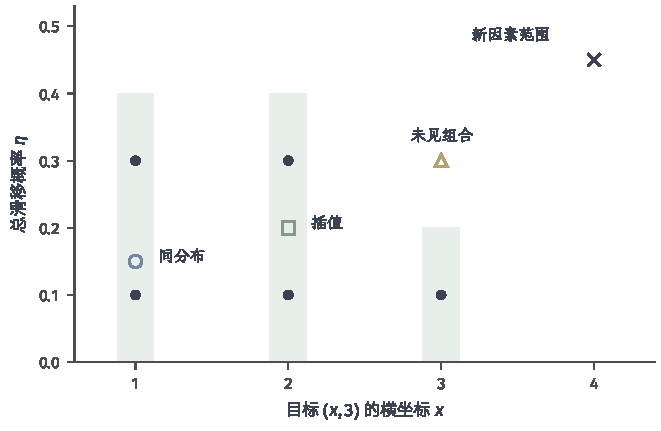
\includegraphics[width=112.000mm]{figures/10-reinforcement-learning/03-task-expansion-and-trustworthiness/matplotlib/rl-transfer-task-plane.pdf}
  \caption{目标位置与移动噪声的教学任务平面。竖向浅带表示离散目标坐标下的总体噪声支持，实点为有限训练样本，其他点形区分留出任务类型。插值只沿噪声轴解释，不把离散网格目标当成连续位置；所有点与支持范围均为教学设定。}
  \label{fig:rl-transfer-task-plane}
\end{figure}

这里“未见”相对于有限样本，“支持外”相对于声明的总体，二者不是同义词。若原总体本来就独立抽取目标与噪声，$(3,0.3)$可能只是在训练清单中缺席，而不在总体支持之外。组合测试必须说明所依据的是边缘支持、联合支持还是经验清单。

% Outline: 6.3.2
\subsection{目标与奖励变化下的可复用知识}
\label{sec:rl-transfer-reward-change}

先单独改变奖励：保持地图、移动规律和终止规则，只把沿途地标的得分换掉。旧转移模型仍可用于规划，旧价值却已经按原奖励计过分，不能直接解释新任务。若希望复用已有轨迹的长期后果，我们可以先记录经过哪些地标、付出多少步成本，再由新任务分别给这些事件赋权。

为使重新赋权可计算，设所有任务有共同$S,\mathsf A,T,\gamma$以及一致的观测、动作和终止语义。用共同的$d$维特征$\bm\phi(s,a,s')$记录一次转移中的事件，用$\bm w_c$记录任务$c$给各事件的权重。如果奖励属于这组特征的线性组合，就有
\begin{equation}
  R_c(s,a,s')=\langle\bm\phi(s,a,s'),\bm w_c\rangle,
  \qquad \bm\phi,\bm w_c\in\mathbb R^d.
  \label{eq:rl-transfer-linear-reward}
\end{equation}
内积把每个事件特征乘以对应权重再求和，因而把不变的事件描述与变化的评价规则分开。$R_c(s,a,s')$是给定这次转移后的期望奖励；再按后继状态概率平均，才得到$R_c(s,a)=\mathbb E_{s'\sim T(\cdot\mid s,a)}R_c(s,a,s')$。奖励样本$r_t$仍可有随机性，不能把上述期望当作每次实际反馈。

在固定策略下，保存未来各特征的期望折扣总量，就能用新权重重新计分。这一对象称为\term{后继特征}（successor features, SF）。对于教学路径，若前两步分别出现$\bm\phi_0=(1,0)^\top$、$\bm\phi_1=(0,1)^\top$，之后特征为0，那么$\gamma=0.9$时后继特征为$(1,0.9)^\top$；权重$(2,-1)^\top$给出价值$1.1$，换为$(0,3)^\top$则给出$2.7$。变化的是评价标准，而不是路径分布。

这个重新计分的例子固定了路径分布。若把得分地标改成一到达就吸收的新终点，后续访问也会改变，旧后继特征就不能直接使用。可以保留固定吸收出口而只改地标奖励，或重新学习包含新终止机制的后继特征。第~\ref{sec:rl-transfer-value-training}~节将从折扣求和推导这种分解，并说明多条已有策略的后果如何用于逐状态选动作。原始后继特征框架研究的也是共同动力学下的奖励迁移\scite{rl6-barreto2017-successor}

即使新奖励可表示，策略库也可能没有掌握通往新目标的行为。保存了正确的后果表示，只能评价已有行为及其可用组合，不等于已经拥有新任务的最优行为。

% Outline: 6.3.3
\subsection{动力学变化下的可复用知识}
\label{sec:rl-transfer-dynamics-change}

现在固定终点和计分规则，只改变移动噪声。进入终点仍得1，但窄路上的滑移可能使原路线更难到达。若这种变化都由一个风参数$\eta$控制，可以保留碰撞规则和模型族$T_\eta$，重新确定参数：$\eta$已给出时直接代入规划，$\eta$未知时用反馈估计。这样复用的是模型结构，不是原来那一组转移概率。

例如，在没有边界或障碍干扰的测试位置，偏离意图可以从后继位置直接辨认。令其指示量$X_j\sim\operatorname{Bernoulli}(\eta)$，独立重置采样$n$次后，用偏离比例$\widehat\eta=n^{-1}\sum_jX_j$估计风参数。独立性使和的方差等于$n\eta(1-\eta)$，取平均再除以$n^2$，所以估计方差为$\eta(1-\eta)/n$。把该参数用于全图，还需要风机制处处相同，并正确合并撞墙后留在原位的概率。墙边的不同滑移可能产生相同后继位置，此时反馈未必能直接给出$X_j$，不能照搬偏离次数估计。

共享模块可以表达“几何碰撞规则相同，风模块变化”；平滑模型可以要求，在指定参数范围内，$\eta$的差异趋于0时，同一状态动作下转移分布的$\ell_1$差异也趋于0。前者减少重复估计的对象，后者给出参数插值的依据；要得到数值误差界，还须限定参数差能使转移差增大多少，两者都不是从网络参数共享自动推出的事实。一般有限表格转移要估计约$|S||\mathsf A|(|S|-1)$个自由概率，单个风参数只估计一个量，但这个维数比较不包含辨识它所需的访问成本。

反例更直接：在同一可见岔路，两个动作分别通向奖励1和0的区域；第二个任务将两个动作的物理效果互换，图像与奖励标记完全不变。旧策略仍选原来的动作，回报由1变为0。旧后继特征预测它会访问奖励区域，因而同样失效；仅修改奖励权重不能把错误转移改对。这个单步例是从导航提取的教学简化，取消滑移与步成本。

即使新旧转移接近，也要检查这种单步误差对长期价值的影响。固定同一策略$\pi$，在共同状态动作空间上比较$T_c$和$T_{c'}$，先假设两者有相同的条件期望奖励$R(s,a)$且$|R|\leq R_{\max}$。以$\sup_{s,a}\lVert T_c-T_{c'}\rVert_1\leq\delta$限制所有相关状态动作上的转移差异；取上确界是为了防止某个策略会访问的位置被平均误差掩盖。两条Bellman关系相减后，继续价值之差贡献第一项，转移之差作用于有界价值贡献第二项：
\[
 \lVert V_c^\pi-V_{c'}^\pi\rVert_\infty
 \leq \gamma\lVert V_c^\pi-V_{c'}^\pi\rVert_\infty
      +\gamma\delta\,\frac{R_{\max}}{1-\gamma}.
\]
这里使用了$\lVert V_{c'}^\pi\rVert_\infty\leq R_{\max}/(1-\gamma)$，以及转移概率差作用于有界函数时的$\ell_1$界。把第一项移到左侧，再除以$1-\gamma$，得到$\gamma\delta R_{\max}/(1-\gamma)^2$。折扣越接近1，越远的后果进入评价，单步差异也可能积累得越大。

共同计分规则不一定给出共同均值奖励。“进入终点得1”虽未改变，到达概率变化仍会改变$R_c(s,a)$。若两者都受同一$R_{\max}$约束，价值界还须加入$\lVert R_c-R_{c'}\rVert_\infty/(1-\gamma)$。这些界限定的是固定策略及全相关状态动作上的误差，训练参数范围内较小的平均预测误差既不能替代一致界，也不能证明范围外参数仍满足它。

% Outline: 6.3.4
\subsection{观测与动作接口变化下的可复用知识}
\label{sec:rl-transfer-interface}

把地图颜色换掉，并不一定改变小车的物理位置；交换左右动作标签，则会改变同一输出命令的控制效果。对一段“右、右、上”的命令序列，单纯换色后物理轨迹可以完全不变，交换命令后却可能向相反方向移动，甚至使命令不再合法。因此观测编码与动作命令应分别对齐。

要判断换接口后是否仍是同一个控制问题，可以比较对应状态上执行对应动作的后果。设$e_c(o)$把新观测编码成原策略所需的决策表示，$m_c(a)$把原语义动作$a$转换成新环境命令，$f_c$把新任务状态对应到原任务状态。这里$m_c$与图\ref{fig:rl-transfer-components}中的$g_c$具有不同方向：$m_c$把原策略动作映为新命令，$g_c$再把新命令映为物理动作。若两任务使用同一物理动作集合，保持物理效果要求$g_c(m_c(a))=g_0(a)$；这只要求在复用动作范围内找到相匹配的命令，不要求$g_c$为双射或存在全局逆。下式的$T_0,T_c$按各自环境的命令索引，已包含相应命令的物理效果。对原任务中的任意相关后继集合$B$，$f_c^{-1}(B)$收集映射到$B$的新任务状态。一个精确复用的充分条件是奖励保持，并且到达这些对应集合的概率相等：
\[
 T_c\!\left(f_c^{-1}(B)\mid s,m_c(a)\right)
 =T_0\!\left(B\mid f_c(s),a\right)
\]
等式需对所有相关状态、合法动作和后继集合$B$成立，还要由$e_c$保留会改变目标动作选择的观测差别、由$m_c$保持动作合法性。左侧在新任务执行映射后的命令，右侧在原任务执行原动作；两者比较的是控制后果，而不是图像或向量的外观相似。图~\ref{fig:rl-transfer-interface}~把观测编码、策略决策、命令映射和执行分别标出。

\begin{figure*}[t]
  \centering
  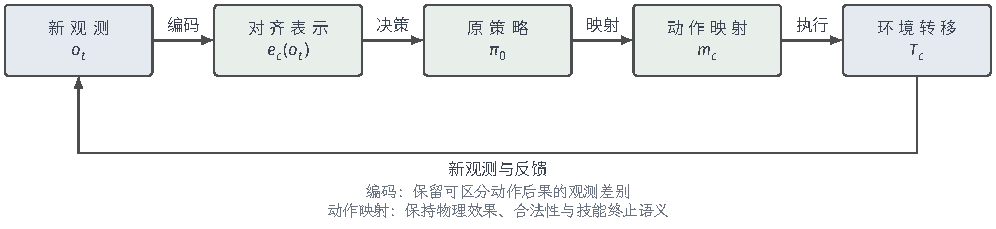
\includegraphics[width=168.575mm]{figures/10-reinforcement-learning/03-task-expansion-and-trustworthiness/tikz/rl-transfer-interface.pdf}
  \caption{观测和动作接口的迁移。观测编码需要保留动作后果预测所需的状态差别，命令映射需要保留物理效果与合法性；任何一侧缺少对应关系，原策略都不能原样解释新接口。图为上述充分条件的原创结构示意。}
  \label{fig:rl-transfer-interface}
\end{figure*}

对于技能，还要把启动状态映射到原启动集，把“到达出口”映射到相同的终止事件。只映射原始动作，而忽略技能结束条件，可能导致高层策略等待一个永远不会到来的反馈。

有限日志未必能唯一确定这些映射。若日志只记录“上”和“下”，左右动作交换前后与全部记录相容；图像重建也无法辨认未试过命令的含义。需要增加有区分力的动作记录，或者提供可信的接口说明。控制充分表示与目标量可识别性的区别见第~\ref{chap:rl-information}~章：同尺寸接口、感知相似度和重建成功都不够。

% Outline: 6.3.5
\subsection{组合与支持外任务所需的额外假设}
\label{sec:rl-transfer-composition}

训练时见过“远终点、无风”和“近终点、有风”，并不意味着已经见过“远终点、有风”。若目标模块只改变奖励、风模块只改变转移，且二者接口独立，模型可以组合这两种知识；若有一个仅在远终点且有风时出现的障碍，原来的两项任务却完全不能揭示它。

把这一区别写成集合关系，令$c=(g,\eta)$。边缘支持$\operatorname{supp}(p_g)$、$\operatorname{supp}(p_\eta)$分别表示总体允许哪些目标和风参数；联合支持$\operatorname{supp}(p_{g,\eta})$表示总体允许哪些目标与风的配对。一个允许配对的两个分量必然各自允许，所以
\[
 \operatorname{supp}(p_{g,\eta})
 \subseteq \operatorname{supp}(p_g)\times\operatorname{supp}(p_\eta),
\]
反向包含不一定成立，两个各自允许的分量未必能配对。\term{组合泛化}（compositional generalization）是在已学因素之间使用未见配对，而不只是识别每个因素。其依据可能是$T_c=T_\eta$、$R_c=R_g$等因子分解，但还需保证组合后观测、动作和终止接口仍成立；这些关系不能由两个单因素测试自动推出。

可以构造两个生成器：它们在已见组合上给出完全相同的地图，只在“远且有风”时分别保持通路或封闭通路。任何只用现有训练组合的算法面对两者取得同分布的训练交互记录，因而不能仅凭这些记录确定新组合是否可通行。增加同一组合的轨迹数量无法消除这个歧义。

未见组合仍由已见因素组成；若引入训练范围外的新动作效果，就连该因素怎样作用于环境也没有从已有训练任务的交互记录中确定。要进一步外推，需要可识别的机制、适用范围明确的平滑性或结构不变性。测试应分别留出组合和因素范围，才能知道支持的是哪一种能力；任务数量多本身并没有给出这些结构关系。

% Outline: 6.4
\section{可复用决策知识的训练}
\label{sec:rl-transfer-training}

前面回答了“什么可以复用、复用到哪里”，接下来要回答“怎样从经验中把这些可复用的知识学出来”。例如多种风向下收集的状态转移记录可以训练一个以风为条件的转移模型，多目标轨迹可以训练一个以目标为条件的价值函数，但两者拟合的对象并不相同。可学习的对象包括表示、模型、价值和策略；而任务随机化、条件化、蒸馏、目标重标记等则是将任务、交互记录或教师动作分布用于这些训练目标的手段，可以组合使用，但都仍受前面共享条件与任务支持的约束。

% Outline: 6.4.1
\subsection{训练任务与经验的构造}
\label{sec:rl-transfer-data}

训练导航任务时，可以随机抽取目标坐标和风强度，也可以用程序生成地图；后者还需检查连通性、合法动作和终止规则。任务产生后，仍要由收集策略真正走出轨迹。因此，训练记录的采样分成两层：按$q(c)$抽任务，再由任务内策略$\beta_c$访问状态动作。折扣采样下，用归一化占用度量$d_c^{\beta_c}(s,a)$描述访问概率，联合经验权重便是$q(c)d_c^{\beta_c}(s,a)$。提高某任务的抽取频率只改变第一个因子，不保证它的关键窄路已被充分访问。

改变$q$还改变了各任务对损失的贡献。若希望保留$p_{\text{训练}}$下的平均目标，就需要用概率或密度比$p_{\text{训练}}(c)/q(c)$重新加权，使按$q$采样的期望恢复为所需期望。这要求$p_{\text{训练}}$相对于$q$绝对连续，即训练目标允许的任务不能落在$q$从不采样的范围；离散时，每个$p_{\text{训练}}(c)>0$的任务都须有$q(c)>0$。重加权不能补回未采任务，过大的权重还会增加估计方差。课程学习若偏向当前较难的任务，应报告这种目标权重变化，不能只描述为增加训练次数。这里的密度比只恢复同一任务条件目标的外层权重，不校正任务内行为策略改变造成的轨迹分布差异。共享条件和绝对连续性成立时，重要性加权可以变换期望的积分分布；有限样本保证还须控制权重大小、损失矩及实际采样依赖。相关跨分布分析可参考\BookChapterRef{chap:transfer-learning-theory}{卷3《基础、理论与可信性》“迁移学习的可学习性”章}。

有些失败轨迹无需重新交互，就能回答另一个目标的问题。\term{事后经验回放}（hindsight experience replay, HER）把轨迹实际达到的位置当作替代目标，重算该目标下的反馈，再交给离策略学习器。它重新解释了已经发生的转移，没有制造另一条物理轨迹\scite{rl6-andrychowicz2017-her}

例如，教学轨迹从$(1,1)$出发，依次到达$(2,1)$、$(3,1)$和$(4,1)$，没有到达原目标$(4,3)$。用新目标$g'=(3,1)$，设到达目标得1、之前每步得$-0.04$，则前两条转移的奖励由$(-0.04,-0.04)$改为$(-0.04,1)$。若新任务到达目标立即结束，第二条转移的终止标记必须同时改为1，后续从$(3,1)$继续移动的记录不能接在这条新回合后作为有效经验。图~\ref{fig:rl-transfer-relabel}~区分真实采集与离线重标记。

\begin{figure*}[htbp]
  \centering
  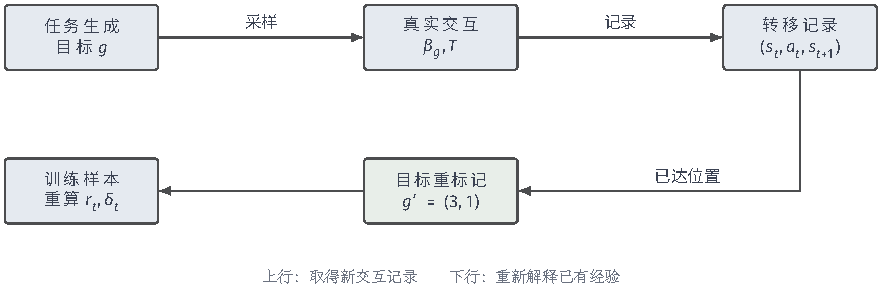
\includegraphics[width=149.296mm]{figures/10-reinforcement-learning/03-task-expansion-and-trustworthiness/tikz/rl-transfer-relabel.pdf}
  \caption{任务生成与目标重标记的两条训练记录构造路径。上行产生真实轨迹，下行重算已有轨迹的目标、奖励和终止标记；重标记箭头不回连环境，因而不增加真实状态动作覆盖。原理据HER，具体导航路径为本章教学构造。}
  \label{fig:rl-transfer-relabel}
\end{figure*}

重标记的语义有效性至少要求：目标不改变非终止物理转移，奖励及目标相关终止信号可按记录重算，动作在新解释中仍合法。若开门目标同时改变门是否锁住，就不能把旧转移当作新目标样本。即使语义有效，随机环境中的选择偏差仍是另一个问题。

设教学单步任务的同一个动作以各$1/2$概率落在左、右地标，且目标不影响转移。真实左目标下成功概率为$1/2$；如果只把“实际落在左边”的记录重标成左目标，再用这些记录估计该动作的左目标成功率，就得到1。每条保留记录都可能真实发生，但条件选择删除了失败分支。确定性动力学可避免这种特定的随机结果选择问题，随机环境则需检查重标记分布或采用适当校正；“目标不改变转移”本身不能证明估计无偏。

重标记$m$个目标会把每条原始记录扩成至多$m$条训练记录，奖励重算约需$O(m)$次调用。增加的是训练计算与目标覆盖，不是$m$倍独立环境证据。

% Outline: 6.4.2
\subsection{可复用状态表示的训练}
\label{sec:rl-transfer-representation-training}

在多个任务间共享一个状态表示，看似总能节省学习，实际上需要小心一个陷阱。不同终点的任务都需要辨认障碍的位置，障碍位置与地图几何可以共享；但在同一个岔路口，它们可能需要截然相反的动作。如果价值或策略只收到相同的观测表示，又没有目标坐标或任务描述作为其他条件，就无从区分该往哪走。因此所谓“任务不变表示”只要求共同的控制要素保持一致，而不要求不同任务的观测与目标描述被压成同一表示；那些会改变动作选择的任务变量，必须在编码器或其后的价值、策略中留有入口。

这个入口可以放在不同位置。共享编码器$\bm z=e_{\bm\theta}(o)$只处理观测，由后续价值或策略另接任务描述$c$；任务条件表示$\bm z=e_{\bm\theta}(o,c)$在编码时就使用目标。模块化表示$\bm z=(e_{\bm\theta}(o),e_{\bm\omega_c}(o,c))$则把共同几何与任务特定的观测编码或转移特征分开，其中$\bm\omega_c$是特定模块参数。三者都可向$Q(\bm z,a,c)$、$\pi(a\mid\bm z,c)$或潜在转移模型供给表示，表~\ref{tab:rl-transfer-representations}~在这些共同用途下比较共享位置与训练条件。

\begin{table*}[t]
  \centering\small
  \begin{tabularx}{\linewidth}{@{}>{\raggedright\arraybackslash}p{18mm}*{5}{>{\raggedright\arraybackslash}X}@{}}
    \toprule
    设计 & 共享部件 & 任务特定部件 & 训练信号 & 任务权重 & 适用条件\\
    \midrule
    共享编码器 & 感知与几何表示 & 条件头或独立头 & TD误差、策略梯度、预测 & 显式$q(c)$ & 编码未混淆目标任务需区别对待的观测\\
    条件表示 & 编码规则和参数 & 描述$c$或历史变量 & 条件价值、控制与预测 & 相同总量下检查各任务 & 描述语义及条件支持兼容\\
    模块化表示 & 共同子模块及组合器 & 风、传感器等模块 & 模块预测与端到端控制 & 可按模块或任务平衡 & 分解与组合接口成立\\
    \bottomrule
  \end{tabularx}
  \caption{三种表示设计。训练信号可以组合，但“参数共享”只描述实现，不能替代控制充分性证明。各列为本章机制归纳。}
  \label{tab:rl-transfer-representations}
\end{table*}

以共享编码器接入评论家为例，训练要让当前动作价值与一步反馈加继续价值一致。一条经验给出的目标为
\[
  y_t=r_t+\gamma(1-\delta_t)
      \max_{a'}\overline Q(e_{\overline{\bm\theta}}(o_{t+1}),a',c).
\]
其中$\delta_t$表示任务真正终止，最大值在后继状态的合法动作中比较继续回报；终止后不再自举。最小化$\tfrac12(Q(e_{\bm\theta}(o_t),a_t,c)-y_t)^2$惩罚当前预测与该目标的残差，梯度通过评论家进入编码器，目标网络在此次梯度中固定。重建损失可帮助感知，但重建成功不等于仍能区分会改变动作后果的观测；还需结合控制目标和充分性条件检查哪些动作后果能被区分。

在一个教学单步岔路中，目标左与目标右需要相反动作。若两项任务的价值或策略接收完全相同的决策表示，任何确定策略都只能满足其中一项；加上一个目标位即可消除这个表示冲突。另一方面，若左任务占采样的$90\%$，总体正确率$90\%$的常向左策略可能完全放弃右任务。这是任务权重造成的平均优势，不是两项任务都获得迁移。

训练计算随编码器前后向成本和样本数增长；多头设计还随任务头数量增加存储，模块化则增加组合与路由成本。诊断时应报告分任务回报、目标位消融与匹配容量的独立模型，区分关键观测差别被抹去、容量不足和优化冲突。总体损失下降不能回答这些不同问题。

% Outline: 6.4.3
\subsection{可复用环境模型的训练}
\label{sec:rl-transfer-model-training}

同一地图上不同风向的轨迹，都受到共同碰撞几何约束，却有不同偏移概率。模型可让共享模块处理几何，再由任务变量确定偏移。令$\widehat T_{\bm\theta,\bm\omega_c}(s'\mid s,a,\bm z_c)$预测下一状态的分布，其中$\bm\theta$为共享参数，$\bm\omega_c$为可选任务特定参数，$\bm z_c$来自描述或历史推断。若另学条件期望奖励与观测分布，分别用$\widehat R$和$\widehat K_o$表示。$\widehat R$预测奖励的条件均值，不是奖励概率分布；生成完整反馈还须规定奖励分布及其与后继状态、观测、终止标记的联合关系。仅拟合转移并没有得到包含全部反馈的模拟器。

在完全可观测、有限离散状态的长度$H$轨迹上，可以检查模型给真实后继状态多大概率。训练提高记录中各步条件转移概率的乘积，等价于最小化负对数似然；对数把各步概率的乘积变成和，负号使低概率预测受到较大惩罚。先对一条轨迹的$H$步平均，再按任务抽样$q$和收集策略的轨迹分布平均，得到
\begin{equation}
 \mathcal L_{\text{模型}}
 =\mathbb E_{c\sim q}\mathbb E_{\tau\sim p_c^{\beta_c}}
 \left[-\frac1H\sum_{t=0}^{H-1}
 \log\widehat T_{\bm\theta,\bm\omega_c}
 (s_{t+1}\mid s_t,a_t,\bm z_c)\right].
 \label{eq:rl-transfer-model-loss}
\end{equation}
模型以已记录的$s_t,a_t$为条件，只拟合后继分布，不把收集策略的动作概率拟合成动力学。经验目标用采到的任务和轨迹平均近似上述期望，再对模型参数求梯度。本式固定$H$并按任务平均；若回合长度不同，按回合平均和按步平均会给任务不同权重，需要另行选定。在相同训练样本、采样分布和权重下，较低训练负对数似然表示模型在这一评分上的改善，尚不能证明模型在未访问位置也正确。

图~\ref{fig:rl-transfer-model}~展示共同几何与任务条件模块如何组合。完全共享模型相当于忽略$\bm\omega_c,\bm z_c$；完全独立模型则为每项任务各拟合全部参数。模块化减少的是共同几何的重复估计，仍需估计新风向，不能以共享参数比例推算目标样本效率。

\begin{figure*}[htbp]
  \centering
  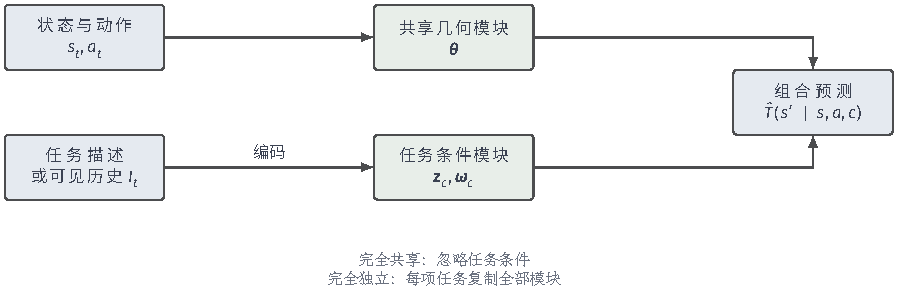
\includegraphics[width=151.987mm]{figures/10-reinforcement-learning/03-task-expansion-and-trustworthiness/tikz/rl-transfer-model.pdf}
  \caption{任务条件环境模型。状态动作进入共享模块，描述或历史进入任务模块，两者共同决定转移预测；奖励、观测头仅在确实训练时增加。图为本章模型参数化的原创示意，不表示所有环境都满足这种分解。}
  \label{fig:rl-transfer-model}
\end{figure*}

用前述一维风参数检验这个目标。在8次可辨认滑移的独立教学试验中观察到2次偏离，似然为$\eta^2(1-\eta)^6$，负对数似然便是$-2\log\eta-6\log(1-\eta)$。在$0<\eta<1$内令导数$-2/\eta+6/(1-\eta)=0$，得到$\widehat\eta=1/4$；目标在两端趋于无穷且二阶导数为正，因此该点是最小点。随后把估计送入共同碰撞模型，计算各位置转移；从测试位置扩大到全图，仍依赖同一个风参数处处适用的结构假设。

训练时知道$c$，部署时却只有历史，是一个额外推断问题。应训练从可见历史到$\bm z_c$的编码器，并在测试中只给这些历史；不能把真实风标签作为隐蔽输入。固定日志上的训练成本约为训练记录数乘单样本模型前后向成本，模型内规划还要乘候选动作序列数及前瞻深度。未覆盖风向、传感器变化和反复滚动的误差累积，都可能使训练似然较好的模型产生错误策略。

% Outline: 6.4.4
\subsection{可复用价值与策略的训练}
\label{sec:rl-transfer-value-training}

表示和转移模型确定之后，还需要按目标来评价动作。同一个岔路通往不同终点时，“向左好不好”取决于要去哪里，因此价值的输入里必须含有目标$g$。如果为每个目标单独存一张价值表，目标一多就无法承受，也无法推广到没见过的目标。\term{通用价值函数逼近器}（universal value function approximator, UVFA）的做法是用一个函数$Q_{\bm\theta}(s,a,g)$统一表示不同状态、动作和目标下的价值；目标条件MDP把$g$纳入任务描述，使这一输入有明确含义\scite{rl6-schaul2015-uvfa}。

训练时从任务$g$的行为策略取得转移，按相同目标确定奖励和终止，再拟合TD目标$r_t+\gamma(1-\delta_t)\max_{a'}\overline Q(s_{t+1},a',g)$。其中最大值比较后继状态的合法动作，表示继续控制的最高估计回报；真正终止时继续项为0。当前预测与目标的残差用于更新参数，执行时也必须查询相同的$g$。多目标共同训练改变了拟合范围，没有取消TD学习的覆盖和估计条件。

实现这种条件价值时，可以由共享评论家联合表示所有目标，也可以共享特征、为各已见任务设置独立输出头；模块化策略则分别处理几何、目标或控制模式。多头的任务编号本身不能解释新目标，UVFA接受连续坐标也不保证能外推到未训练范围。每次TD更新要计算当前价值和目标动作值，有限动作枚举成本随$|\mathsf A|$增长；连续动作不能逐一枚举，需要行动者或其他最大化近似。

条件价值仍需学习不同目标的计分结果。若希望按新奖励重用同一策略的长期后果，可以先记录未来访问次数；这与前面后继特征的两步例子相连，这里进一步说明该记录怎样计算和训练。其前身\term{后继表示}（successor representation, SR）记录固定策略下未来访问各状态的期望折扣次数。有限状态时，$M^\pi(s,u)$描述从$s$出发对状态$u$的访问量：
\[
 M^\pi(s,u)=\mathbb E_\pi\!\left[\sum_{t\geq0}\gamma^t
       \mathbb I\{s_t=u\}\mid s_0=s\right].
\]
指示量只在访问$u$时计1，折扣和区分到达早晚，期望则平均策略与转移的随机结果。若$\bm T^\pi$为策略诱导的状态转移矩阵，拆出$t=0$时的当前访问，余下从下一状态继续，便得
$\bm M^\pi=\bm I+\gamma\bm T^\pi\bm M^\pi$，从而
$\bm M^\pi=(\bm I-\gamma\bm T^\pi)^{-1}$。矩阵的谱半径是其特征值绝对值的最大值；随机矩阵$\bm T^\pi$的谱半径不超过1。乘以$\gamma<1$后，$\gamma\bm T^\pi$的每个特征值绝对值都小于1，因而1不是它的特征值，0也就不是$\bm I-\gamma\bm T^\pi$的特征值。该矩阵因此可逆，方程给出确定的访问量。SR一般存储$|S|^2$个数；若只需重新评价特定事件，可以把每个状态的指示量换成低维事件特征，得到SF\scite{rl6-dayan1993-successor}

SF需要按当前动作比较价值，因此条件中固定首动作$a$，此后再遵循$\pi$。下面对所有相关转移限制特征范数，保证无限折扣和有界；这个上确界条件是求期望和交换极限的依据，不是平均特征较小就能代替的条件。

\begin{definition}[固定策略的后继特征]
 \label{def:rl-transfer-sf}
 给定状态空间$S$、行动空间$\mathsf A$、非空合法动作集$\mathsf A(s)$及转移核$T$，各空间与核采用相容的可测结构，取共同折扣$0\leq\gamma<1$。令正整数$d\geq1$，可测特征映射$\bm\phi:S\times\mathsf A\times S\to\mathbb R^d$在所有合法转移上满足
 $\sup_{s\in S,a\in\mathsf A(s),s'\in S}\lVert\bm\phi(s,a,s')\rVert_2\leq C_\phi<\infty$。
 固定合法平稳Markov策略$\pi$，其中$\pi(\cdot\mid s)$是在$\mathsf A(s)$上的概率核；其后继特征为
 \begin{equation}
 \bm\psi^\pi(s,a)=
 \mathbb E_\pi\!\left[
 \sum_{t=0}^{\infty}\gamma^t\bm\phi(s_t,a_t,s_{t+1})
 \,\middle|\,s_0=s,a_0=a\right].
 \label{eq:rl-transfer-sf}
 \end{equation}
 首动作按条件强制执行，之后服从$\pi$。
\end{definition}

定义得到的是事件总量，还需证明它乘上权重后确实等于动作价值。对随机奖励，另假设各状态动作下的绝对一阶矩有共同有限上界；有界奖励样本是一个充分条件，这保证折扣奖励和可积。记$\bm\phi_t=\bm\phi(s_t,a_t,s_{t+1})$，由特征有界性，
$\sum_{t\geq0}\gamma^t\lVert\bm\phi_t\rVert_2\leq C_\phi/(1-\gamma)$；
对固定有限$\bm w_c$，条件期望奖励的绝对折扣和也有上界
$C_\phi\lVert\bm w_c\rVert_2/(1-\gamma)$。因此可以用支配收敛把部分和的极限移入期望，并用条件期望先把$r_t$替换成转移条件期望奖励。依次得到
\begin{align}
 Q_c^\pi(s,a)
 &=\lim_{N\to\infty}\mathbb E_\pi
       \left[\sum_{t=0}^{N}\gamma^t R_c(s_t,a_t,s_{t+1})
       \mid s_0=s,a_0=a\right]\notag\\
 &=\lim_{N\to\infty}\left\langle
       \mathbb E_\pi\left[\sum_{t=0}^{N}\gamma^t\bm\phi_t
       \mid s_0=s,a_0=a\right],\bm w_c\right\rangle\notag\\
 &=\langle\bm\psi^\pi(s,a),\bm w_c\rangle.
 \label{eq:rl-transfer-sf-value}
\end{align}
第二步使用式~\eqref{eq:rl-transfer-linear-reward}~与有限和、内积的线性性，第三步使用前述可积性。SF不含奖励权重，却仍依赖$T$和$\pi$；在新任务换掉转移后，原式右侧不再使用正确的轨迹分布。

价值分解解释了SF的用途，但完整轨迹求和不便于逐步训练。与标量价值一样，把首步特征和以后特征分开，利用马尔可夫性先平均后继状态、再按固定策略平均下一动作，就得到向量Bellman方程：
\begin{equation}
 \bm\psi^\pi(s,a)=
 \mathbb E_{s'\sim T}\left[\bm\phi(s,a,s')
 +\gamma\mathbb E_{a'\sim\pi(\cdot\mid s')}\bm\psi^\pi(s',a')\right].
 \label{eq:rl-transfer-sf-bellman}
\end{equation}
方程把长时程事件总量化成一步目标，可以用转移样本近似。表格情形从覆盖相关状态动作的行为策略$\beta$取得转移，计算
$\bm y_t=\bm\phi_t+\gamma\sum_{a'}\pi(a'\mid s_{t+1})\widehat{\bm\psi}(s_{t+1},a')$，
再令$\widehat{\bm\psi}(s_t,a_t)$向$\bm y_t$移动步长$\alpha$。终止时继续项为0。若仅采样一个$a'\sim\pi$，则以该样本替代动作期望。这里评价的是固定$\pi$，不能无说明地把下一动作改成最大值。表格每次更新的向量运算为$O(d|\mathsf A|)$，采样下一动作时为$O(d)$；网络实现还包含前后向成本。

SF训练不需要新奖励权重，但新任务计分需要它。若$\bm w_c$未知，可比较目标奖励样本$r_j$与特征预测$\bm\phi_j^\top\bm w_c$，最小化残差平方和
$\sum_j(r_j-\bm\phi_j^\top\bm w_c)^2$。平方惩罚预测偏差，样本和形成经验拟合目标；要使这项$d$维线性最小二乘拟合有唯一解，训练特征矩阵还需满列秩，有噪声时唯一拟合值仍不保证等于真实权重。若目标描述直接给出权重，则不需要这一步目标反馈，但仍须有共同动力学下训练好的SF。

有了多条策略的SF，就能按同一个新奖励计算各自的动作价值。固定调用一条策略可能错过另一条策略在某个状态的有用动作。\term{广义策略改进}（generalized policy improvement, GPI）在每个状态比较所有库内策略的动作价值，再选择估值最高的合法动作；动作执行后可以重新选择，不必整回合锁定同一条策略。先对策略取最大值，再对动作取最大值，是要利用库内任一策略提供的较高继续价值。下面的保证因此以已有策略为参照，不与未知的新任务最优策略比较\scite{rl6-barreto2017-successor}

\begin{theorem}[有一致估计误差的广义策略改进]
 \label{thm:rl-transfer-gpi}
 在同一个状态集$S$及各合法动作集$\mathsf A(s)$均有限且非空、逐步奖励有界、折扣$0\leq\gamma<1$的MDP中，取正整数$m$和$\varepsilon\geq0$，给定$m$条合法平稳Markov策略
 $\{\pi_1,\ldots,\pi_m\}$。若对每个$i=1,\ldots,m$及所有合法状态动作均满足
 $|\widehat Q^{\pi_i}(s,a)-Q^{\pi_i}(s,a)|\leq\varepsilon$，
 定义确定性策略的动作映射
 \[
 \pi(s)\in\argmax_{a\in\mathsf A(s)}\max_i\widehat Q^{\pi_i}(s,a),
 \]
 并固定平局规则；对应的策略核为该动作上的点质量，则
 \begin{equation}
 Q^\pi(s,a)\geq\max_iQ^{\pi_i}(s,a)
                -\frac{2\varepsilon}{1-\gamma}.
 \label{eq:rl-transfer-gpi-bound}
 \end{equation}
\end{theorem}

要证明逐状态拼接后仍有保证，先限制一次近似贪心选动作的损失，再沿Bellman备份累计它。令
$f(s,a)=\max_iQ^{\pi_i}(s,a)$、$\widehat f(s,a)=\max_i\widehat Q^{\pi_i}(s,a)$；
一致误差保证$|f-\widehat f|\leq\varepsilon$。由$\pi$的贪心定义，
\[
 f(s,\pi(s))\geq\widehat f(s,\pi(s))-\varepsilon
 =\max_a\widehat f(s,a)-\varepsilon
 \geq\max_a f(s,a)-2\varepsilon.
\]
两个$\varepsilon$分别来自所选动作的估值误差和最佳动作的估值误差。用$\mathcal B^\pi$表示动作价值的Bellman评价算子；下一状态按$\pi$选出的$f$值至多比最大值低$2\varepsilon$，平均并折扣后有
\begin{align*}
 \mathcal B^\pi f
 &\geq R+\gamma T\max_a f-2\gamma\varepsilon\\
 &\geq \max_i\{R+\gamma T\mathbb E_{a'\sim\pi_i}Q^{\pi_i}\}
           -2\gamma\varepsilon\\
 &=f-2\gamma\varepsilon\geq f-2\varepsilon.
\end{align*}
其中$T$表示对后继状态取期望；第二行用“每个后继状态上的最大值至少覆盖任一$\pi_i$的动作平均”，再对策略取最大。Bellman单调性以及
$\mathcal B^\pi(f-b)=\mathcal B^\pi f-\gamma b$给出
$(\mathcal B^\pi)^k f\geq f-2\varepsilon\sum_{j=0}^{k-1}\gamma^j$。
有限折扣MDP中，$\mathcal B^\pi$是压缩算子，左侧迭代收敛到$Q^\pi$；右侧几何级数收敛到$1/(1-\gamma)$，于是得到式~\eqref{eq:rl-transfer-gpi-bound}。损失容限来自一致估值误差的逐步积累。深度网络的平均TD损失较小，并没有因此满足全状态动作上误差至多$\varepsilon$的条件。

\begin{example}[两条绕障策略的新奖励评价]
 \label{ex:rl-transfer-sf-routes}
 以下简化保留导航地图与固定吸收出口$(4,3)$，取消滑移与步成本，沿途地标允许重复计分。取特征为进入$(1,3)$、进入$(4,1)$、首次进入出口的三个指示量，吸收后特征为0，$\gamma=0.9$。两条确定策略从起点分别走“上、上、右、右、右”和“右、右、右、上、上”；离开这两条路线的状态可用任一固定合法规则补全策略。

 上路在$t=1$经过第一个地标，$t=4$进入出口；下路在$t=2$经过第二个地标，$t=4$进入出口。因此从起点执行各自首动作并继续原策略时，
 \[
 \bm\psi^{\pi_1}=(0.9,0,0.6561)^\top,\qquad
 \bm\psi^{\pi_2}=(0,0.81,0.6561)^\top.
 \]
 新权重$\bm w=(1,2,1)^\top$给出两条完整路线的回报$1.5561$与$2.2761$。固定调用下路优于固定调用上路；GPI则需为每个候选首动作查询每条补全策略的SF，再逐状态选择，不能仅凭这两个整路线数字实现。

 当SF精确时，GPI在各状态不会劣于库内任一策略；当所有动作价值一致误差至多为教学假设$\varepsilon=0.01$时，本定理给出的逐动作损失容限为$0.2$。从状态开始执行GPI也满足同样的保守容限：近似贪心至多损失$2\varepsilon$，后续至多损失$2\gamma\varepsilon/(1-\gamma)$。这些保证没有比较库外最优策略；地标重复奖励甚至可能使有益循环优于直接离场。
\end{example}

策略库有$m$条策略、每个SF为$d$维时，直接GPI查询约需$m|\mathsf A|$个SF输出和$O(m|\mathsf A|d)$次乘加。相比每个新奖励都从头学习，它复用了后果计算；相比单次策略前向，它增加了查询成本。新奖励残差、新动力学误差和策略库缺失各自需要额外分析，不能全塞进未经测量的$\varepsilon$。

GPI保留多份后果表示，查询成本随策略库增长。如果部署希望用一个网络保存多个教师的已有行为，可以在教师访问的状态上拟合其动作分布，这称为\term{策略蒸馏}（policy distillation）。共同动作接口下，用教师分布到学生分布的KL散度衡量拟合差异，再按任务采样$q$和状态分布$\nu_c$平均：
\[
 \mathcal L_{\text{蒸馏}}=
 \mathbb E_{c\sim q,\,s\sim\nu_c}
 D_{\mathrm{KL}}\!\left(\pi_c^{\text{教师}}(\cdot\mid s)
       \,\Vert\,\pi_{\bm\theta}(\cdot\mid s,c)\right).
\]
$\nu_c$来自教师或其他收集行为，梯度只更新学生。教师固定时，KL中的教师熵不随学生参数变化，因而可以用交叉熵训练。一个教学二动作教师给出$(0.8,0.2)$，学生用softmax把两个动作分数（logit）转换为概率$(0.5,0.5)$，则交叉熵对这两个分数的梯度为$(-0.3,0.3)$，梯度下降提高第一动作概率。压缩教师省去部署时多个网络的独立调用，却没有保存教师从失败中学习的过程，日志外状态仍可能失配。原始策略蒸馏工作主要研究多任务策略压缩\scite{rl6-rusu2016-distillation}

蒸馏保存的是已有行为；若部署允许少量梯度更新，还可以保存一个经这些更新后能取得较高回报的参数起点。\term{模型无关元学习}（model-agnostic meta-learning, MAML）正是把更新后的任务损失作为训练初始化的目标。“模型无关”指可用于不同可微参数模型，不是强化学习中的“无模型”分类。令$L_c(\bm\theta)=-J_c(\pi_{\bm\theta})$为负回报，由$U_c$按规定的任务内训练样本和预算执行更新。在允许的参数范围内最小化更新后负回报，等价于提高更新后回报：
\begin{equation}
 \min_{\bm\theta}\ %
 \mathbb E_{c\sim p_{\text{训练}}}
 \mathbb E_{D_c^{\text{内}}\sim Q_{c,n}^{\pi_{\bm\theta}}}
 L_c\!\left(U_c(\bm\theta,D_c^{\text{内}})\right).
 \label{eq:rl-transfer-meta-objective}
\end{equation}
这里$Q_{c,n}^{\pi_{\bm\theta}}$是按内层采集协议取得整批记录的联合律，$n$是该协议规定的样本数；它与单条理论轨迹律不同；在下述可微似然条件下，以$q_{c,n}^{\pi_{\bm\theta}}$表示整批记录相对于固定支配测度的质量函数或密度。两个期望分别平均训练任务和当前初始化策略产生的内层训练样本，避免把某一次幸运采样当成适应能力。训练抽取任务$c$，收集$D_c^{\text{内}}$并更新后，还要用新策略在同一任务另采$D_c^{\text{外}}$估计更新后回报，再据此调整初始化。外层记录也参与初始化训练，不是选择结束后的最终测试样本。这个经验过程优化的是约定预算后的表现，不要求初始策略立即解决所有任务\scite{finn2017}

调整初始化需要知道它怎样影响更新后的参数。先固定内层训练样本，令可微更新为$\bm\theta'=\bm\theta-\alpha\nabla\widehat L_c^{\text{内}}$；它对初始参数的导数矩阵（Jacobian）为$\bm I-\alpha\nabla_{\bm\theta}^2\widehat L_c^{\text{内}}$，描述初始参数的微小变化怎样传到更新后参数，其中$\nabla_{\bm\theta}^2\widehat L_c^{\text{内}}$是内层损失的二阶导数矩阵。链式法则把更新后损失梯度传回初始化，给出条件导数
\[
 \nabla_{\bm\theta}L_c(\bm\theta')
 =\left(\bm I-\alpha\nabla_{\bm\theta}^2\widehat L_c^{\text{内}}\right)^\top
       \nabla_{\bm\theta'}L_c(\bm\theta').
\]
在强化学习中，内层训练样本的采集律本身依赖$\bm\theta$；若要求式~\eqref{eq:rl-transfer-meta-objective}~的完整梯度，还存在
$L_c(\bm\theta')\nabla_{\bm\theta}\log q_{c,n}^{\pi_{\bm\theta}}(D_c^{\text{内}})$
这一采样分布项。把已采轨迹当作固定张量、对普通策略梯度代理反传，并不自动得到无偏的完整高阶梯度。必须说明使用的估计器及省略项；具体目标任务更新见第~\ref{sec:rl-transfer-gradient-adaptation}~节。

\begin{example}[固定样本求导为何会漏掉采样分布项]
  \label{ex:rl-transfer-sampling-gradient}
  只取一条记录，令$D=(Y)$，其中$Y\sim\operatorname{Bernoulli}(p_\theta)$、$p_\theta=\sigma(\theta)$，并设$F(\theta,D)=Y$。记录固定后，$F$没有显式参数依赖，因此$\partial_\theta F(\theta,D)=0$。但总体目标为$\mathbb E_\theta F=p_\theta$，故
  \[
    \frac{\mathrm d}{\mathrm d\theta}\mathbb E_\theta F
       =p_\theta(1-p_\theta).
  \]
  在$\theta=0$处，这个导数为$1/4$。差异完全来自参数改变了会采到什么记录：Bernoulli记录的得分为$Y-p_\theta$，采样分布项的期望为
  \[
    \mathbb E_\theta[Y(Y-p_\theta)]=p_\theta(1-p_\theta).
  \]
  这里没有内层Hessian，却已经出现固定记录导数与完整期望导数的差别。元学习还要叠加内层更新对参数的影响，因此不能仅由是否计算二阶导数判断采样项是否完整。
\end{example}

表~\ref{tab:rl-transfer-behavior-objects}~比较四种保存方式。技能还需保存启动集$I_o$、内部策略$\pi_o$及终止概率$\beta_o$；其发现机制见第~\ref{chap:rl-learning}~章。这里的关键区别是保存已有动作规律、可重加权的后果，还是未来更新的起点。

\begin{table*}[t]
 \centering\small
 \begin{tabularx}{\linewidth}{@{}>{\raggedright\arraybackslash}p{22mm}*{3}{>{\raggedright\arraybackslash}X}@{}}
  \toprule
  对象 & 保存什么 & 目标任务还需做什么 & 接口与边界\\
  \midrule
  价值与SF & 指定行为的长期后果 & 重加权、策略改进或价值重估 & 奖励类、共同转移、策略语义\\
  蒸馏策略 & 教师动作分布 & 条件调用或额外适应 & 观测与动作编码对齐；日志外误差\\
  可迁移初始化 & 适合更新的参数起点 & 用获准目标任务样本做有限更新 & 步长、梯度质量、更新后评价\\
  技能库 & 启动集$I_o$、可读状态或历史、$\pi_o$、$\beta_o$ & 选择、组合或调整内部控制 & 动作效果、持续时间与终止含义兼容\\
  \bottomrule
 \end{tabularx}
 \caption{行为知识的四种保存方式。技能“能够运行”只验证部分接口，不保证适合新目标；表中没有把它们视为互斥算法类别。}
 \label{tab:rl-transfer-behavior-objects}
\end{table*}

% Outline: 6.5
\section{目标任务策略的形成}
\label{sec:rl-transfer-policy-formation}

前面几节准备好了可复用的知识，但到了一个具体的新任务，策略还要“落地成形”。如果新终点坐标已经直接给出，训练好的目标条件策略也许查询一下就能选出动作；但若只知道终点、不知道风向，同一个模型还得依据新收到的反馈判断当前的移动规律，才能决定怎么走。所以可复用知识只是形成目标策略的起点。新证据可以改变记忆、任务后验或网络参数中的某一个，而能否继续收集证据，则取决于协议给了多少交互权限。下面先说明任务描述和交互历史怎样一步步约束“当前是哪个任务”，再依次考察零样本、固定参数、允许梯度更新和持续交互等不同权限下如何据此选择动作。

% Outline: 6.5.1
\subsection{从显式描述与交互历史形成任务信息}
\label{sec:rl-transfer-belief}

考虑导航任务的一个独立教学变体：终点已知，风向$c\in\{\text{左风},\text{右风}\}$在整个试验期间固定，先验各为$1/2$。终点描述没有给出风向参数。在一个获准的测试位置，某个试探动作产生可见“右偏”的概率在两项任务中分别为$0.2$和$0.8$。观察一次右偏会改变对风向的判断；反复撞上同一堵墙，如果两种风都只留下“位置未变”，就可能完全没有区分力。数字仅用于说明似然更新，未作为基准网格的新转移解。

为了把“右偏后更相信右风”写成可计算的判断，先设当前物理状态可见，历史为
$I_t=(s_0,a_0,r_0,\delta_0,\ldots,s_t)$，其中$\delta_t$记录动作$a_t$之后的终止事件。有限任务集合上的\term{任务信念}（task belief）
$b_t(c)=\mathbb P(c\mid I_t)$是给定已见证据后对任务的概率分布。显式描述可以约束先验或直接确定某些任务分量；它与历史证据应进入同一条件化过程，而不是相互替代。若初始状态分布也随任务变化，看到$s_0$时便已有证据：描述条件下的先验为$p_0(c)$时，$b_0(c)\propto p_0(c)\mu_{0,c}(s_0)$，不能无条件沿用$p_0$。

令$\ell_c(s_{t+1},r_t,\delta_t\mid s_t,a_t)$为任务$c$中可用模型给出的联合似然。任务固定、奖励及终止模型正确，且动作仅由已记录历史和独立随机数选择时，贝叶斯公式给出
\begin{align}
 b_{t+1}(c)
 &=\frac{b_t(c)\,
     \ell_c(s_{t+1},r_t,\delta_t\mid s_t,a_t)}
 {\sum_{\widetilde c\in\mathcal C}b_t(\widetilde c)\,
     \ell_{\widetilde c}(s_{t+1},r_t,\delta_t\mid s_t,a_t)}.
 \label{eq:rl-transfer-belief-update}
\end{align}
分子用新反馈在任务$c$下出现的概率，对原有可信度重新加权；分母对所有候选任务求和，使更新后的概率之和为1。它也是所见反馈的预测概率，需大于0。推导中，联合概率包含
$b_t(c)\pi(a_t\mid I_t)\ell_c(\cdot)$；动作概率在各候选任务间相同，故在归一化时消去。若收集者另知隐藏任务并据此选动作，却未记录它读取的任务标签或参数，就不能不加分析地消去它。

前述右偏观测给出
$b_{t+1}(\text{右风})=0.8/(0.8+0.2)=0.8$。若独立重置到测试位置后又观察一次右偏，则后验为
$0.8^2/(0.8^2+0.2^2)=16/17$。任务后验改变的是对固定对象的认识，不是风向本身。若物理状态也隐藏，就不能继续使用包含真实状态的$I_t$。此时应改用可见历史
$I_t^{\mathrm{vis}}=(o_0,a_0,r_0,\delta_0,\ldots,a_{t-1},r_{t-1},\delta_{t-1},o_t)$，并维护
$b_t(s,c)=\mathbb P(s_t=s,c\mid I_t^{\mathrm{vis}})$。更新时先按任务$c$的转移核对旧状态求和，再用新观测、奖励与终止反馈的联合似然重新加权；这要求给出正确的任务转移模型和可见反馈模型。不能用一个任务向量代替状态滤波而省去这些条件。

右偏例子只有两个候选任务，可以逐项更新。精确枚举有限任务的单步更新需要$|\mathcal C|$次似然计算；状态同时隐藏时还包含状态转移求和。任务空间很大时，这种逐项计算通常改由历史编码器近似完成。编码器还需要训练信号，使输出保留会改变奖励、后继观测预测或动作选择的历史差别。图~\ref{fig:rl-transfer-belief-loop}~因此区分执行时的推断控制闭环与训练时的监督或变分目标，不能把网络输出直接当成真实任务标签。

\begin{figure*}[htbp]
 \centering
 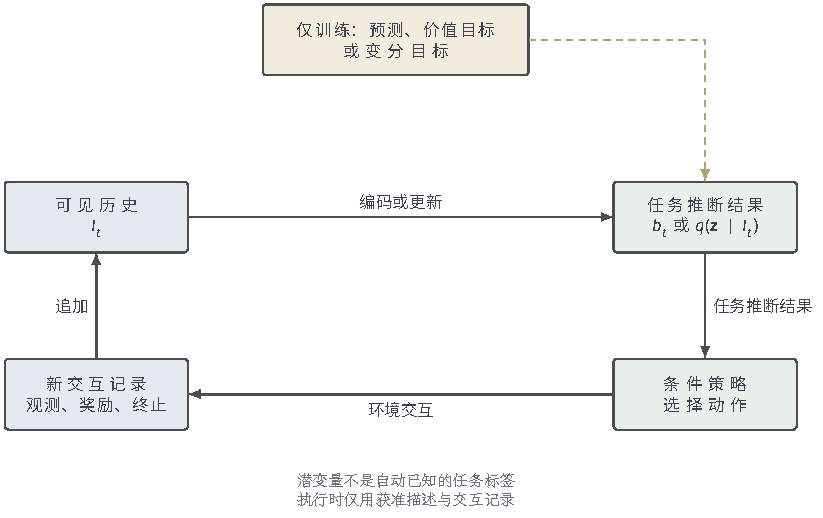
\includegraphics[width=139.446mm]{figures/10-reinforcement-learning/03-task-expansion-and-trustworthiness/tikz/rl-transfer-belief-loop.pdf}
 \caption{任务推断结果与行为的闭环。实线为执行时实际传递的观测、任务估计与动作，虚线为训练时用于塑造推断器的目标；传给策略的任务推断结果可以是精确后验、近似分布或普通历史编码，三者不能仅因向量维数相同就互换。图为本章机制的原创归纳。}
 \label{fig:rl-transfer-belief-loop}
\end{figure*}

\term{概率上下文元强化学习方法}（PEARL）把已收集的转移作为上下文$\mathcal C_t$，由编码器参数$\bm\varphi$形成潜变量$\bm z$的近似分布$q_{\bm\varphi}(\bm z\mid\mathcal C_t)$。从这个分布抽取$\bm z$后，策略据此选择动作，评论家据此评价动作。其原始设计把每条转移对应的高斯因子相乘并归一化，适合任务固定、转移可按集合处理的情形；离策略回放用于训练评论家与策略，编码器通过价值学习信号提取任务线索，相对先验的KL正则则约束潜变量分布。训练依次抽取任务、该任务上下文与回放转移，更新相应损失；部署收集获准的少量转移，更新潜变量分布，再抽样形成行为。这里保存的是任务潜变量的近似条件分布，不是已知真实风标签\scite{rl6-rakelly2019-pearl}

同样需要从历史提取任务线索，\term{变分贝叶斯自适应深度强化学习方法}（VariBAD）选择按时间递归编码历史，并通过变分目标学习潜变量。训练中的解码器用潜变量重建同一任务的奖励和转移，预测损失要求编码器保留能预测所记录奖励与后继观测的历史差别；KL项约束近似后验与先验或先前后验的差异。条件策略读取后验参数，而不只读取一个任务点估计，并以跨回合回报学习何时试探以取得新反馈、何时按现有后验选择高回报动作。执行时不需要调用训练用解码器做模型内规划。因此，训练中有预测解码器，并不能推出部署时采用基于模型的规划\scite{rl6-zintgraf2020-varibad}

回到右偏例子，现在要检验的是近似推断能否支持决策，而不是再演算一次贝叶斯公式。精确二任务模型给出$0.8$这一可核后验；近似编码器则需检查同类历史下的反馈预测与校准，不能要求某个潜变量坐标也恰好等于$0.8$。PEARL式抽样让行为在一个抽取的任务假设下连贯执行，VariBAD式条件策略可以依据分布的不确定性决定是否再探测；是否学到有效探索，仍依赖训练任务与反馈。前者要计算上下文因子及条件策略，后者要逐步维护循环状态和后验参数；两者训练还包含评论家或解码器成本，不能只比较策略前向次数。

存在比近似误差更根本的限制。构造两个终点隐藏的教学任务：在最后一次岔路选择前，预算内所有获准动作的状态、奖励和终止分布完全相同；最终向左或向右分别只在其中一个任务成功，先验各为$1/2$。任何历史编码器可读取的交互记录具有相同分布，因此最终选择左的概率在两任务中相同。若该概率为$p$，平均成功率为$\tfrac12p+\tfrac12(1-p)=1/2$。增加网络容量不能提高这项上限。只有允许额外访问会显示终点线索的状态，或提供带区分力的描述，主动辨识才可能改变预算内能够取得的任务线索。

% Outline: 6.5.2
\subsection{无目标任务更新数据下的零样本策略}
\label{sec:rl-transfer-zero-shot}

目标坐标已给出、状态编码和目标描述语义与训练一致时，策略形成可以只是一次条件查询：
$a_t\sim\pi_{\bm\theta}(\cdot\mid s_t,g)$，或
$a_t\in\argmax_a Q_{\bm\theta}(s_t,a,g)$。若同时给出可解释的新奖励权重，还可计算
\[
 a_t\in\argmax_a\max_i
 \langle\widehat{\bm\psi}^{\pi_i}(s_t,a),\bm w_g\rangle.
\]
后一种调用先用新权重给每项候选策略的后果计分，再对每个动作取策略库中的最高估值，最后选取估值最高的动作。它复用了SF策略库，不需要目标奖励样本；但共同动力学、终止与特征语义，以及第~\ref{thm:rl-transfer-gpi}~定理的估计条件仍不能省略。

这里沿用第~\ref{sec:rl-transfer-budget}~节的零样本口径：禁止用目标反馈更新权重、任务记忆或选择检查点，无论更新发生在回合内还是跨回合。当前观测仍然可见，否则连位置控制都无法执行；预先约定的物理状态滤波与未知任务辨识应分开报告。若把偏移或奖励反馈送入历史编码器，据此推断风向并改变后续控制，就已发生任务适应，即使尚未结束第一个回合、也没有一次反向传播。

可以在同一训练模型上固定目标坐标格式、动作选择规则和推理次数，分别测试图~\ref{fig:rl-transfer-task-plane}~中的$(1,0.15)$、$(3,0.3)$和$(4,0.45)$任务。它们依次代表支持内新任务、未见因素组合和范围外因素；训练参数与测试权限完全相同，变化的是所检验的任务关系。应分别报告三组零样本回报，而不是把它们合成一个“新任务平均分”。

若输入只有新编号3，条件网络无法由数字推断它代表哪个终点。若新目标需要从未形成的控制方式，或目标设备交换了左右动作接口，旧策略库即使每条策略都能前向计算，也可能没有一个合法有效的候选。零样本能力来自已有知识与描述之间成立的关系，不来自关闭更新开关本身。

% Outline: 6.5.3
\subsection{参数固定条件下基于上下文的策略适应}
\label{sec:rl-transfer-context-adaptation}

设想同一个隐藏风向的任务连续运行两个回合：第一回合先试探一下风往哪边吹，第二回合就根据观察到的偏移去绕开障碍。这已经是一种“适应”——行为根据新任务的反馈发生了改变。问题是：能不能在完全不改网络权重的前提下做到这一点？答案是可以，前提是策略必须把前一回合的证据保留下来，而不是每一步只看当前位置。此时真正变化的不是参数，而是历史记忆以及由它形成的任务估计。一个循环网络若在训练中见过足够多不同风向的任务，就可能把“如何利用历史推断任务并据此行动”这一学习过程本身，写进它的内部状态里。

\term{循环元强化学习方法}（RL$^2$）以循环策略把快速学习过程放入内部状态\scite{rl6-duan2016-rl2}
执行时固定网络参数$\bm\theta$，令
\begin{align}
 \bm m_t
 &=f_{\bm\theta}(\bm m_{t-1},o_t,a_{t-1},r_{t-1},\delta_{t-1}),\notag\\
 a_t&\sim\pi_{\bm\theta}(\cdot\mid\bm m_t).
 \label{eq:rl-transfer-rl2}
\end{align}
首步的上一动作、奖励与终止标记使用约定的空值。终止标记说明上一动作结束了物理回合；环境此时重置位置，但同一任务的$\bm m$继续保留。只有切换任务、开始新的独立适应试验时，才重置任务记忆。训练时在多项任务上优化跨多个回合的总回报，参数更新发生在这个较慢的过程里。目标覆盖同一任务的多个回合，早期探测的成本才可能由后续回合的收益补偿。

图~\ref{fig:rl-transfer-rl2-memory}~把固定参数外框与可变记忆分开。在前述教学风任务中，可构造一个实现贝叶斯更新的记忆器：初始记忆存右风概率$1/2$，第一个回合观察右偏后存$0.8$，第二回合用新概率选择路线。这个例子证明固定参数可以实现适应，不声称训练出的RL$^2$必然等价于精确贝叶斯推断。

\begin{figure*}[htbp]
 \centering
 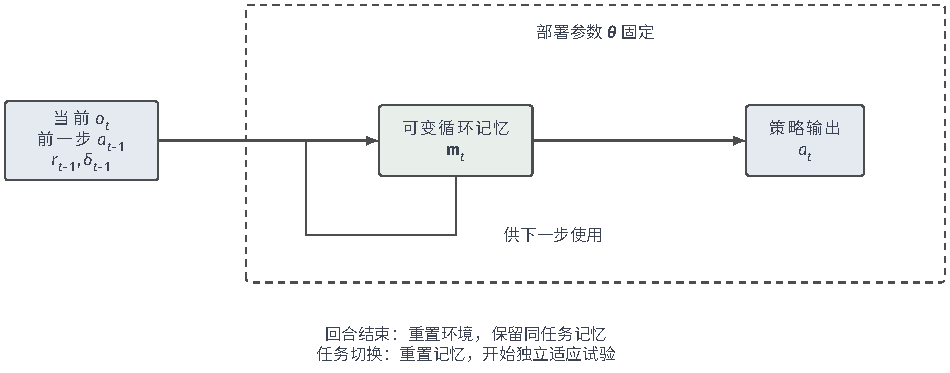
\includegraphics[width=160.800mm]{figures/10-reinforcement-learning/03-task-expansion-and-trustworthiness/tikz/rl-transfer-rl2-memory.pdf}
 \caption{固定参数中的可变记忆。输入包含当前观测及上一动作对应的奖励和终止标记；同任务回合结束仅重置物理环境，任务改变才重置记忆。图据RL$^2$的交互协议重绘，贝叶斯数值例是本章构造，不是其训练结果。}
 \label{fig:rl-transfer-rl2-memory}
\end{figure*}

若希望模型从已有算法的学习记录中学会怎样改进行为，可以保留记录中的回合顺序，而不只收集算法最终的动作。\term{算法蒸馏}（algorithm distillation, AD）据此从源强化学习算法的多回合学习记录抽取长序列，以自回归动作预测拟合
$-\sum_t\log\pi_{\bm\theta}(a_t\mid I_t)$\scite{rl6-laskin2023-ad}
输入历史包括观测、动作与奖励，训练样本保留从探索到改进的顺序；部署时把自身新经历追加到历史，固定参数继续预测动作。它模仿的是学习过程中的行为变化，而前述策略蒸馏通常只压缩已训练教师的行为。

AD的标签来自学习过程，未必是任务最优动作。\term{决策预训练Transformer}（decision pre-trained Transformer, DPT）改用任务内上下文和查询状态，预测教师给出的最优动作。训练时从任务$c$抽取上下文$D_c$和查询$s$，拟合
$-\log\pi_{\bm\theta}(a_c^*(s)\mid s,D_c)$；连续动作可使用相应密度损失。理想化地，若标签确为各任务最优动作、任务分布与上下文生成方式正确覆盖测试情形，监督条件分布会对仍与上下文相容的任务作后验混合。这解释了与后验采样的联系，不是任意有限网络都具备贝叶斯最优探索的保证\scite{rl6-lee2023-dpt}

\Needspace{26\baselineskip}
如果没有最优动作标签，也可以直接用交互回报训练记忆条件策略。\term{自适应智能体}（adaptive agent, AdA）在程序化任务空间中安排逐步调整的训练课程，训练带记忆的智能体，使跨回合反馈影响行为；其训练信号是交互回报，而非给定最优动作标签\scite{rl6-bauer2023-ada}

上下文还可以先用于评价动作，再用于形成策略。\term{可扩展上下文Q学习}（scalable in-context Q-learning, S-ICQL）利用世界模型生成任务提示，训练读取上下文的动作价值$Q$与状态价值$V$。它结合偏向高价值样本的expectile目标和优势加权策略提取。前者先拟合一个偏重高价值样本的状态价值，后者再用估计优势给策略训练样本赋权；两者解决的是不同步骤。测试上下文可以来自协议规定的在线交互或离线记录。

expectile中的“不对称”可以直接从残差看出。令待拟合状态价值为$v$，残差为$u=Q-v$；当$u>0$时，当前$v$低估了该动作价值。取$\omega\in(1/2,1)$，对正残差使用权重$\omega$，对负残差使用权重$1-\omega$，便会更重地惩罚这种低估。一个教学例有两个等权价值样本0和2，取$\omega=0.75$。在$v\in[0,2]$内，目标为
\[
  \frac12\left[0.25v^2+0.75(2-v)^2\right],
\]
导数为$v-1.5$，最小点为1.5。它高于样本均值1，却低于最大样本2，也不等于这两个样本的75\%分位数2。因而expectile是通过不对称平方惩罚改变拟合位置，并没有把最大样本直接认定为真实最优值。随后用$Q-V$构造估计优势并提高相应动作的策略拟合权重，是另一项操作。

Vintix II进一步考察DPT式决策预训练怎样使用多领域、含噪行为记录。它用这些记录构造上下文，再以示范者动作重标记监督目标，区分上下文中实际发生的行为与希望预测的动作。它的动作头不是一次回归出最终动作，而是学习怎样把噪声逐步变成动作。下面用$u\in[0,1]$表示动作生成过程的时间；$u$不是环境交互时刻$t$。

训练时，先由上下文与查询得到Transformer隐向量$\bm z_j^{\mathrm{hid}}$，再由高斯噪声$\bm x_0$和示范动作$\bm a^\star$构造线性路径
\[
  \bm x_u=(1-u)\bm x_0+u\bm a^\star.
\]
这条路径关于$u$的速度为$\bm a^\star-\bm x_0$。动作头以$\bm x_u,u,\bm z_j^{\mathrm{hid}}$为条件预测速度向量场，并用平方误差使预测速度接近这个标签。监督量因此是生成过程中的运动方向，而非把每个中间点直接回归为最终动作。

\begin{samepage}
执行时重新采样$\bm x_0$，沿学得的速度场数值积分，从$u=0$推进到$u=1$，把终点$\bm x_1$作为当前环境时刻的连续动作。用一维教学例可以区分训练与生成：噪声起点为0、示范动作为2时，路径为$x_u=2u$，训练速度标签为2。若学得的速度处处等于2，用Euler法手算两步、每步长度$0.5$，便依次得到0、1、2。真实动作分布中的速度场还依赖当前位置与上下文；这个例子只说明为何训练预测速度、执行却要积分生成动作。该方法同时研究在线与离线的上下文使用，其跨领域结果仍受所用低维观测、控制接口和训练任务支持约束，不能改写成任意视觉任务的通用保证\scite{rl1-polubarov2026-vintix}
\par
\end{samepage}

表~\ref{tab:rl-transfer-context-methods}~按上下文记录与策略形成方式对照这些方法。它们都能在固定参数下利用新上下文，但训练信号分别来自交互回报、学习历史中的动作、教师标签或条件价值估计。这些差别决定了模型能够从训练任务的交互记录及动作标签中学到什么，不能仅以是否使用Transformer判断适应机制。

\begin{table*}[t]
 \centering\small
 \begin{tabularx}{\linewidth}{@{}>{\raggedright\arraybackslash}p{20mm}*{4}{>{\raggedright\arraybackslash}X}@{}}
  \toprule
  方法 & 上下文内容 & 训练样本来源 & 目标反馈 & 策略提取\\
  \midrule
  RL$^2$ & 观测、前动作、奖励、终止 & 多任务在线跨回合交互 & 同任务内逐步到达 & 循环记忆条件策略\\
  AD & 按顺序的多回合学习历史 & 源RL算法的学习轨迹 & 追加自身交互历史 & 自回归预测动作\\
  DPT & 任务内转移及查询状态 & 上下文与教师最优动作标签 & 给定上下文或新交互 & 监督条件动作分布\\
  AdA & 跨回合观测、动作与反馈 & 程序化任务、课程与在线RL & 试验内持续反馈 & 记忆条件的RL策略\\
  S-ICQL & 任务提示与交互上下文 & 世界模型提示和离线记录 & 在线或离线上下文 & 条件价值与优势加权策略\\
  Vintix II & 多领域转移上下文 & 含噪记录、示范者动作重标 & 在线或离线上下文 & DPT式条件化与流匹配动作头\\
  \bottomrule
 \end{tabularx}
 \caption{固定参数上下文适应的不同训练信号。各方法的上下文、反馈量和策略提取成本必须单独核对；该表归纳原始方法，不表示使用同一批训练样本得到的实验排名。}
 \label{tab:rl-transfer-context-methods}
\end{table*}

表中的差别并不只在网络输出形式。AD直接拟合学习历史中的动作，S-ICQL先学习条件价值，再按估计优势给策略训练样本加权。二者都可在固定参数下适应，但历史进入决策的训练依据不同\scite{rl1-liu2026-sicql}

这类方法的运行代价不止权重存储。循环策略每步更新固定维度记忆，长序列Transformer在朴素实现中对长度$L$的完整注意力计算为$O(L^2)$；缓存可以减少重复计算，但仍要存储上下文及相关状态。条件价值可能需要额外候选动作评价；Vintix II采用的流匹配动作头还需若干生成步骤\scite{rl1-polubarov2026-vintix}
比较时应报告实际上下文长度、缓存、推理次数与延迟，不把“零梯度步”写成“零适应成本”。

任务边界错误也会改变结果：把前一任务记忆带入下一任务会污染推断，过早清空记忆会丢掉跨回合证据；截断窗口可能删掉唯一的风向线索。学习轨迹若只有无效随机行为，AD无法仅靠动作模仿获得未出现的改进规则；教师标签、世界模型和任务生成器也各有支持限制。训练中学到某种改进模式，并不意味着在任意新任务上都能保证探索和性能单调提升。

% Outline: 6.5.4
\subsection{允许有限梯度更新下的参数适应}
\label{sec:rl-transfer-gradient-adaptation}

前一小节把风向证据写进了记忆、参数始终不动。如果协议还允许修改参数，就多了一条路：把获准取得的目标任务交互记录当作适应训练样本，直接调整策略本身，这就是基于梯度的快速适应。它要估计的是“当前策略参数对目标任务回报的梯度”，而不是去预测任务编号或给风向做分类。其背后的思路常被称为“学会学习”（元学习）：在训练阶段，不只是让策略在各任务上表现好，而是让它的初始参数处在一个“只需在新任务上走几步梯度就能变好”的位置。设任务$c$在适应期间固定，从$\bm\theta^{(0)}=\bm\theta$出发，以当前策略收集$D_c^{(0)}$。对于有限时域折扣回报，令
$L_c(\bm\theta)=-\mathbb E[\sum_{t=0}^{H-1}\gamma^t r_t]$；
终端价值取0。沿用策略梯度的可微性、环境不依赖策略参数及可积性条件，可构造
\begin{align}
 \widehat{\bm g}_c
 &=-\frac1N\sum_{j=1}^N\sum_{t=0}^{H-1}
   \gamma^t\nabla_{\bm\theta}\log\pi_{\bm\theta}
        (a_{j,t}\mid I_{j,t})
   \bigl(G_{j,t}-b(I_{j,t})\bigr),\notag\\
 \bm\theta'&=\bm\theta-\alpha\widehat{\bm g}_c.
 \label{eq:rl-transfer-inner-update}
\end{align}
$N$是独立采集的轨迹数，$G_{j,t}$是轨迹$j$从动作时刻$t$起的折扣回报。把动作的对数概率梯度乘以回报，再对轨迹平均，估计提高高回报动作概率的方向；基线$b$用于减少方差，不能依赖当前所采动作，且在此梯度中视为固定。式中额外的$\gamma^t$来自起点目标的折扣；损失是负回报，所以减去负回报梯度才对应提高回报。该样本梯度可记作
$\nabla_{\bm\theta}\widehat L_c$，但不能通过把环境奖励当成参数的普通可微函数来获得它。

\begin{example}[一次目标任务参数更新]
 \label{ex:rl-transfer-gradient-step}
 将导航末端岔路简化为独立单步教学任务：向右奖励1、向左奖励0，动作概率为
 $p_\theta=\pi_\theta(\text{右})=\sigma(\theta)$，初值$\theta=0$，基线0。收集4次独立试验，假设实际抽到3次右、1次左。对于右动作，
 $\partial_\theta\log p_\theta=1-p_\theta=1/2$；左动作奖励0，贡献为0。于是
 \[
 \begin{aligned}
 \widehat g&=-\frac{3(1/2)}4=-\frac38,\qquad
 \alpha=2,\qquad \theta'=\frac34,\\
 p_{\theta'}&=\frac1{1+e^{-3/4}}\approx0.6792.
 \end{aligned}
 \]
 更新前的真实期望回报为$0.5$，更新后为$0.6792$。这里能够直接算真实值，是因为教学任务的奖励模型已完整给出；实际未知任务需要另采独立评价回合来估计回报。4条记录的经验回报$0.75$既不是更新前真实值，也不能作为更新后性能证明。
\end{example}

执行顺序因此是收集、估计、更新、另行评价。扩展为$K$步时，用
$\bm\theta^{(k+1)}=\bm\theta^{(k)}-\alpha_k\widehat{\bm g}_c^{(k)}$；
每步若按同策略估计，需要由更新后策略新采的轨迹训练样本，复用旧策略的轨迹记录则必须采用适当离策略估计并满足覆盖条件。固定日志不提供未记录动作的反事实回报，允许梯度计算也不会自动补齐这一缺口。

第~\ref{sec:rl-transfer-value-training}~节的MAML外循环还需评价更新对初始化的依赖。保留
$\bm I-\alpha\nabla^2\widehat L_c$是在给定内层样本时反传内循环导数；一阶近似以$\bm I$代替这一Jacobian，减少高阶自动微分开销。二者都还需交代整批训练样本律$Q_{c,n}^{\pi_{\bm\theta}}$的采样分布项是否纳入估计；示例~\ref{ex:rl-transfer-sampling-gradient}~说明，即使固定记录的导数为0，完整期望梯度也可能非零。部署时执行若干普通目标梯度步，本身并不需要再计算元梯度。

表~\ref{tab:rl-transfer-storage}~按新任务记录或估计结果写入的位置比较适应机制。计算成本包括训练所需的反向传播、优化器状态和独立评价，而不只是最终策略推理。

\begin{table*}[t]
 \centering\small
 \begin{tabularx}{\linewidth}{@{}>{\raggedright\arraybackslash}p{19mm}*{4}{>{\raggedright\arraybackslash}X}@{}}
  \toprule
  机制 & 记录或估计的存储位置 & 变化内容 & 重置与可逆性 & 主要代价\\
  \midrule
  上下文适应 & 历史窗口、循环状态 & 新经验与压缩记忆 & 可清空；被截断的历史记录未必可恢复 & 记忆存储、序列前向\\
  任务信念 & 离散概率或后验参数 & 各假设的相对可信度 & 可重置先验；恢复旧后验需保存证据或快照 & 似然、归一化或近似推断\\
  参数适应 & 策略、价值或模型权重 & 梯度及优化器状态 & 有初值快照才可完整回滚 & 前后向、优化器、再评价\\
  \bottomrule
 \end{tabularx}
 \caption{目标任务记录与估计结果的存储位置。这是机制比较而不是互斥分类：后验可作为上下文输入，记忆更新也可与参数更新同时执行。}
 \label{tab:rl-transfer-storage}
\end{table*}

少量样本估计的梯度可能有较大波动，过大步长可能破坏原有行为；模型错配或离策略权重过大还可能使估计方向失真。教学例中的一次改进不能推成一般单调保证。没有获准用于更新的目标任务训练样本、只获准固定参数部署，或探测动作违反可行动作约束时，就不能默认运行这套流程。

% Outline: 6.5.5
\subsection{持续交互下的任务辨识与在线适应}
\label{sec:rl-transfer-identification}

如果未知风向在整个部署期间都固定不变，那么早先收集到的有效观测始终在指向同一个当前任务，持续交互就能让判断越来越准。但这里有一个容易被忽视的陷阱：一个只沿安全边界走、从不经过受风影响位置的策略，可能拿到稳定的回报，却永远辨认不出风向。也就是说，持续交互要想真正减少不确定性，所选的行为必须能带来区分性的证据；而是否值得为此专门去“试探”，还要权衡探测本身的成本与弄清任务后能带来的控制收益——这正是第\ref{chap:rl-learning}章探索与利用张力在任务层面的再现。

把这一取舍简化为独立的两阶段、不折扣教学任务。两种风先验各半；终端安全路线奖励$0.6$，按正确风向选择的捷径奖励1、选错奖励0。直接选择时，捷径期望$0.5$，故安全路线较好。若第一阶段允许付出$0.1$奖励成本，执行一个正确率$0.8$的对称风向探测，再按信号选择捷径，则总期望回报为$-0.1+0.8=0.7$。不探测的策略在第一阶段等待且不扣分，两者使用相同两阶段时域。探测提高了终端决策的期望回报$0.2$，付出成本$0.1$，净收益$0.1$；若探测成本改为$0.3$，原方案就不再值得。

同一个正确率$0.8$的探测，在两种成本下得到不同决策，所以探测反馈的收益必须由它带来的后续回报改变量评价，不能只看任务分类准确率。在线过程可以每收集一小批转移便更新一次后验和策略，也可以逐步更新记忆、偶尔更新参数。当前任务估计影响行为，行为改变后续观测、奖励与终止记录的分布，新记录再更新任务估计或控制规则。只更新后验、只更新参数或同时更新两者，都可能形成这样的闭环，但代价和稳定性不同。

图~\ref{fig:rl-transfer-identification-curves}~刻意把任务辨识误差和控制回报画在两个坐标系中。早期两条曲线同时表现为辨识误差较大、控制回报较低，这一并存现象只提示应检查任务辨识误差是否限制控制；仅凭两条独立设定的解析曲线，不能确定低回报的原因。后来误差已经很低而回报仍未达到目标，则提示还需检查规划或控制。图中的解析曲线只描述一种待检验的诊断情形，不是任何方法的收敛率，也没有假设分类误差可以直接换算成回报。

\begin{figure}[htbp]
 \centering
 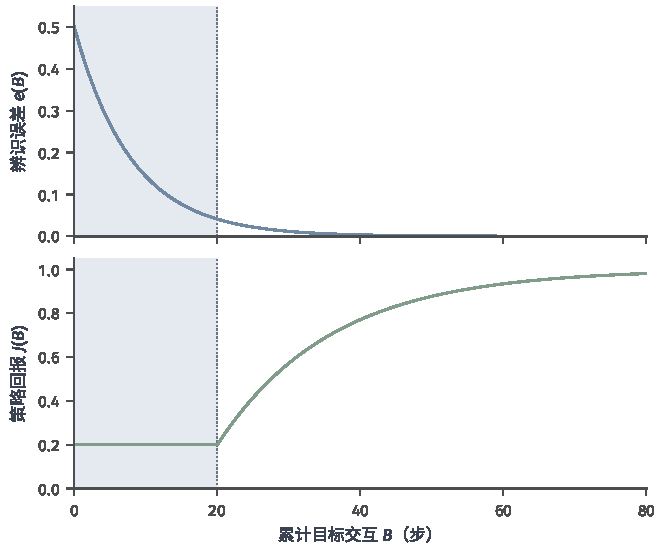
\includegraphics[width=112.000mm]{figures/10-reinforcement-learning/03-task-expansion-and-trustworthiness/matplotlib/rl-transfer-identification-curves.pdf}
 \caption{固定任务下辨识与控制的不同进度。教学解析曲线为$e(B)=0.5e^{-B/8}$和$J(B)=0.2+0.8(1-e^{-\max(B-20,0)/16})$；$B$为累计目标交互步数。竖线$B=20$用于分区说明，非实测拐点，亦非理论阈值。两图共享横轴，不共享纵轴量纲。}
 \label{fig:rl-transfer-identification-curves}
\end{figure}

误差可以按已知测试标签计算，也可以按后验对真实任务的概率或参数偏差计算，报告时需固定一种定义。部署系统没有真实任务标签时，只能用已观测反馈检查预测残差、反馈预测的校准或其他可观察证据；检验任务后验本身的校准仍需真实任务标签，不能把测试者知道的风向反送给策略。实际测量还应改变探测预算，分别检查任务辨识误差是否降低，以及固定同一组任务描述与记录后控制回报是否提高。

探测、回到测试位置、失败恢复和再评价全部消耗资源。更多交互只有在可识别、能到达相关状态且反馈权限充分时才有帮助。若辨识需要越过禁止区域，不能以“学习所必需”为理由默认开放动作；安全探索与约束可行性见第~\ref{chap:rl-trustworthy}~章。

% Outline: 6.5.6
\subsection{任务持续变化下的跟踪与适应}
\label{sec:rl-transfer-tracking}

现在把固定风向改成回合间突变，或让风强度缓慢漂移。上个回合的右偏仍是真实记录，却可能不再代表当前风向。直接把式~\eqref{eq:rl-transfer-belief-update}~用于全部历史，会把已失效的证据累积成过度自信；要继续作贝叶斯推断，需要额外给出任务变化模型，否则应采用明确的跟踪估计。

处理过时证据有几种不同办法。变化检测与重启先检查预测残差是否异常，再丢弃或下调旧模型；滑动窗口只保留最近$W$条记录；历史降权则给年龄为$j$的样本权重$\lambda^j$，其中$0<\lambda<1$。它们分别决定何时停用旧估计、保留多少近期交互记录，以及旧记录随时间减轻多少影响。窗口大或$\lambda$接近1时，稳定阶段估计方差较低，变化后的响应却较慢。例如独立Bernoulli观测在固定参数下，窗口均值的方差为$\eta(1-\eta)/W$；参数突变后，这个均值在旧记录移出前仍混合两种机制。检测阈值还要在误报、漏报和延迟间取舍。

检测出风向变化以后，重新估计和恢复控制仍会损失回报。要累计评价这段代价，需要先规定每次变化后的比较对象。考虑共同有限状态动作空间、共同初始分布$\mu_0$的回合式任务序列，各回合逐步奖励有界。第$k$回合的MDP为$\mathcal M_k$，在该回合内固定，时域为$H$；用不折扣总奖励
$V_{k,0}^{\pi}(\mu_0)=\mathbb E_{\mu_0,\pi,\mathcal M_k}
[\sum_{t=0}^{H-1}r_{k,t}]$，终端价值0。$r_{k,t}$仍按回合内动作时刻编号，与无限折扣目标分别使用。令$\pi_k$是算法基于此前观测、动作与奖励记录选择的本回合行为规则，可以在回合内依靠新历史行动。

\begin{definition}[动态遗憾与静态遗憾]
 \label{def:rl-transfer-regret}
 给定正整数$T,H$及$T$个回合任务，各回合从共同初始分布$\mu_0$启动，采用前述相同的$H$步不折扣总奖励与行动前历史权限。记$V_{k,0}^{\pi}(\mu_0)$为策略$\pi$在第$k$个任务中的期望回报，要求所比较的回报有限；$V_{k,0}^*(\mu_0)$是知道该回合任务模型、仍只按获准历史行动的策略类中的有限最优值。动态遗憾逐回合计算算法策略$\pi_k$比这一最优值少多少，再相加：
 \begin{equation}
 \operatorname{DReg}_T
 =\sum_{k=0}^{T-1}\left[
 V_{k,0}^{*}(\mu_0)-V_{k,0}^{\pi_k}(\mu_0)\right].
 \label{eq:rl-transfer-dynamic-regret}
 \end{equation}
 若比较者必须始终使用同一策略，就在预定的非空固定策略类$\Pi_{\text{固定}}$中，取整段序列累计回报的上确界；假设该上确界有限。相对于这一比较值的静态遗憾为
 \begin{equation}
 \operatorname{SReg}_T
 =\sup_{\pi\in\Pi_{\text{固定}}}
       \sum_{k=0}^{T-1}V_{k,0}^{\pi}(\mu_0)
       -\sum_{k=0}^{T-1}V_{k,0}^{\pi_k}(\mu_0).
 \label{eq:rl-transfer-static-regret}
 \end{equation}
 固定比较策略不随回合改变，可依赖回合内时间与允许观测；不能暗含当回合隐藏任务标签。若另有条件保证最优比较策略存在，上确界可以写成最大值。随机任务序列或随机算法下，另对这些随机性取期望。
\end{definition}

动态比较者在每次变化后都立即知道新的奖励与转移，显著强于部署者。静态比较者只选一个共同规则；算法若成功跟踪变化，甚至可能优于它，故静态遗憾不应解释为适应延迟。两者必须使用相同初始分布；如果还改变初始分布，应把它列入变化机制和评价条件。

动态比较者每回合都能换成当前最优策略，而部署者需要从反馈认识变化。若要使平均每回合差额随回合数增长而趋于0，即取得次线性动态遗憾，就需要约束环境变化或另给关于当前任务参数的提示。例如可限制相邻回合任务改变的次数
$S_T=\sum_{k=1}^{T-1}\mathbb I\{\mathcal M_k\ne\mathcal M_{k-1}\}$，
或者在共同有界奖励尺度下定义
\begin{align}
 B_R&=\sum_{k=1}^{T-1}\sup_{s,a}|R_k(s,a)-R_{k-1}(s,a)|,\notag\\
 B_T&=\sum_{k=1}^{T-1}\sup_{s,a}
 \lVert T_k(\cdot\mid s,a)-T_{k-1}(\cdot\mid s,a)\rVert_1.
 \label{eq:rl-transfer-variation}
\end{align}
每项上确界取相邻回合在所有状态动作上的最大变化，$B_R$累加奖励均值的变化幅度，$B_T$累加转移分布的$L^1$变化幅度。使用全部状态动作，而不只使用当前策略产生的交互记录，是为了限制环境本身的变化；未访问位置的变化也可能影响后续最优决策。变化次数、累计幅度与单次最小可检测幅度不是同一个量。频繁微小漂移可以次数多而累计幅度小；一次大跳变也可能因相关状态不可达而难以检测。是否给出变化提示、提示是否含新任务参数，以及是否已知变化预算，都需单独说明。非平稳学习理论是在这些条件下研究性能，而非取消所有条件后承诺及时适应\scite{rl6-wei2021-nonstationary}

\begin{theorem}[无预告快速变化的两臂下界]
 \label{thm:rl-transfer-linear-regret}
 在$H=1$的教学任务族中，每轮$k$独立均匀抽取
 $C_k\in\{1,2\}$，动作集合为两个臂，奖励为
 $r_k(a)=\mathbb I\{a=C_k\}$。选择动作前不给任何关于$C_k$的线索；选择后可以观察所得奖励。对任何使用过去历史、内部随机源与任务序列独立的随机算法，以知道当轮$C_k$并选择相应臂的策略作动态比较者，有
 \[
 \mathbb E[\operatorname{DReg}_T]=T/2.
 \]
\end{theorem}

\begin{proof}
 令$\mathcal F_k$包含第$k$轮之前的全部动作、奖励及算法已用的随机数。算法还可使用与任务序列独立的新随机数$U_k$，据
 $(\mathcal F_k,U_k)$选择$A_k$。由构造，$C_k$与上述$\mathcal F_k$和本轮新随机数$U_k$独立，且在两臂上均匀分布，因此不论条件动作概率如何，
 对条件概率为正的动作$a$，
 $\mathbb P(C_k=a\mid\mathcal F_k,U_k,A_k=a)=1/2$。
 对动作分支求和便得
 \begin{align*}
 \mathbb P(A_k=C_k\mid\mathcal F_k,U_k)
 &=\sum_{a=1}^2
    \mathbb P(A_k=a\mid\mathcal F_k,U_k)\,\tfrac12\\
 &=\tfrac12.
 \end{align*}
 取全期望，每轮算法的期望奖励为$1/2$。知道当前任务$C_k$的动态比较者选择臂$C_k$，每轮奖励恒为1；它不需要预知任何未来任务。由期望的线性性，
 \[
 \mathbb E[\operatorname{DReg}_T]
 =\sum_{k=0}^{T-1}\left(1-\mathbb E[r_k(A_k)]\right)
 =\sum_{k=0}^{T-1}(1-\tfrac12)=T/2.
 \]
 轮末反馈即使揭示了本轮完整任务，也不能预测独立的下一轮，所以结论不依赖算法的记忆容量、计算时间或参数更新能力。
\end{proof}

这一下界不否认缓慢变化可以跟踪，也不否认预告信号可以帮助决策。它只指出：比较者知道当前最好动作而算法在选择前毫无线索时，无规律快速变化本身足以产生线性代价。静态比较者的期望优势却小得多。令$N_1$为$T$轮中臂1高奖励的次数，最佳固定臂奖励为
$T/2+|N_1-T/2|$；由方差及Cauchy--Schwarz不等式，
$\mathbb E|N_1-T/2|\leq\sqrt{T}/2$。因此同一算法对固定臂的期望静态遗憾至多$\sqrt{T}/2$，而动态遗憾仍是$T/2$。换比较对象就换了结论。

图~\ref{fig:rl-transfer-tracking}~进一步区分变化发生、变化检测和性能恢复三个时刻。检测准确也不等于立即恢复：模型重估、规划与控制学习仍有代价。恢复阈值和观察窗口应提前规定，不能看到曲线后再选最有利时刻。

\begin{figure}[htbp]
 \centering
 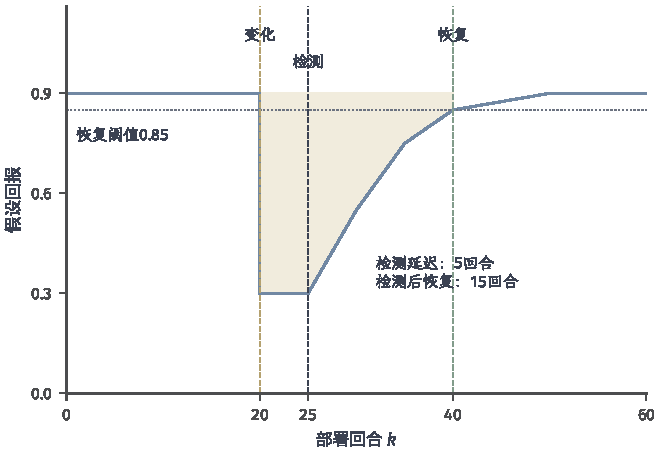
\includegraphics[width=112.000mm]{figures/10-reinforcement-learning/03-task-expansion-and-trustworthiness/matplotlib/rl-transfer-tracking.pdf}
 \caption{变化、检测与恢复的教学时间线。曲线由图源中给定的分段线性控制点生成；变化在回合20，检测在25，首次达到预设回报阈值$0.85$在40。下降、延迟和恢复期间的差额各有含义，非任何算法的实测轨迹。}
 \label{fig:rl-transfer-tracking}
\end{figure}

若系统从不按回合重置，前期动作会影响变化发生时的物理状态，就应使用适合持续过程的平均回报、动态比较规则或跟踪损失，不能原样套用共同$\mu_0$的式~\eqref{eq:rl-transfer-dynamic-regret}。变化期间的决策代价由动态比较规则或跟踪损失衡量；旧能力保留、遗忘和一般持续学习理论可参考\BookVolumeRef{vol:knowledge-learning}{卷8《学习范式：知识的获取、演进与迁移》}中的知识演进与知识迁移部分。

% Outline: 6.5.7
\subsection{任务信息与适应权限的组合边界}
\label{sec:rl-transfer-combinations}

目标坐标已知时，陌生地面仍可能要求估计摩擦参数；隐藏风向没有描述时，记忆中积累的偏移证据也可以改变条件策略，不必改网络权重。前面分别讨论的描述、记忆、梯度更新与持续交互，因此可以出现在同一系统中。描述决定已知哪些任务条件，其他机制决定怎样取得缺少的任务反馈并形成相应估计。

表~\ref{tab:rl-transfer-permissions}~以任务描述及反馈可见条件为行、机制权限为列。每格写的是该组合所需的证据和接口，而非给方法贴一个永久类别标签。

\begin{table*}[t]
 \centering\small
 \begin{tabularx}{\linewidth}{@{}>{\raggedright\arraybackslash}p{18mm}*{4}{>{\raggedright\arraybackslash}X}@{}}
  \toprule
  描述与反馈条件 & 零样本调用 & 上下文更新 & 参数更新 & 持续交互\\
  \midrule
  显式描述 & 描述语义、范围与接口兼容；不读目标反馈学习 & 描述加获准历史；反馈可补描述遗漏 & 描述加日志或新样本；允许反传 & 允许探测描述未给出的动力学；全部计费\\
  隐藏任务 & 依据先验、已给描述及正常控制所需观测选择；不据目标反馈辨识任务或选模 & 历史须含区分性反馈；规定窗口与重置 & 更新样本须支持估计；不使用隐藏标签 & 可达的区分动作、反馈权限与恢复预算\\
  \bottomrule
 \end{tabularx}
 \caption{任务描述、可见反馈与适应权限的组合。各列可同时启用，持续交互规定可采集哪些目标任务记录，不是与记忆或梯度互斥的网络结构。}
 \label{tab:rl-transfer-permissions}
\end{table*}

例如，显式目标加两步梯度更新可以用目标选择损失，再由新转移修正行动者；但两步所用交互、学习率选择和更新后评价仍须纳入预算。隐藏风向加固定参数记忆则可用第一回合判断风向、第二回合选路；它不消耗梯度步，却消耗反馈和上下文。两种组合只有在总交互次数、可读描述与反馈可比时，才有理由比较“适应更快”。

技能复用也遵循这一划分。任务描述或信念决定高层在合法启动集内选哪项技能，技能结束后根据新观测再组合下一项；若允许更新，可以只改高层选择器，也可以调整技能内部控制参数。后者可能改变持续时间与终止分布，应重新检查与高层价值估计的接口，而不能把内部更新当作无影响替换。技能定义与单任务时间抽象仍沿用第~\ref{chap:rl-learning}~章。

比较方法前应同时固定目标交互数、反馈字段、上下文容量、梯度步数及额外计算。主动辨识与基于测试成绩的选模都使用目标任务的交互反馈或测试成绩，不能从预算中删除。适应机制的组合越灵活，实验协议越需要明确。

% Outline: 6.6
\section{迁移结论的验证与修正}
\label{sec:rl-transfer-validation}

最后要问：怎样确认迁移真的发生了，以及它在什么范围内成立？一个模型在新终点上拿到较高回报，可能是真的直接调用了旧知识，也可能是在测试过程中已经偷偷读取了大量新任务的反馈；只报告一个平均成绩，还可能把强风任务上的失败淹没掉。因此，前面陆续给出的共享条件、任务描述与反馈、策略形成机制，都需要在验证环节逐项落实：测试任务从哪里来、反馈何时可见、预算如何累计、与谁作比较。只有把这些交代清楚，才能确定一个分数究竟支持的是哪一项迁移主张。

% Outline: 6.6.1
\subsection{由目标任务适用范围确定任务级数据划分}
\label{sec:rl-transfer-split}

同一风向、同一目标下的轨迹随机分成两组，只检验任务内的新经历。要回答换任务后能否复用，就应先在任务层划分：检验支持内新任务时，留出完整任务身份；检验组合泛化时，留出目标与噪声的指定组合；检验范围外能力时，把相应因素范围从训练和调参任务中排除。每一种划分都对应前面声明的一种目标任务关系。

图~\ref{fig:rl-transfer-split}~按任务、回合、片段三层展示这一差别。同一回合的相邻片段共享物理轨迹，同一任务的不同回合共享隐藏参数；把它们都视为独立任务会严重夸大证据量。

\begin{figure*}[htbp]
 \centering
 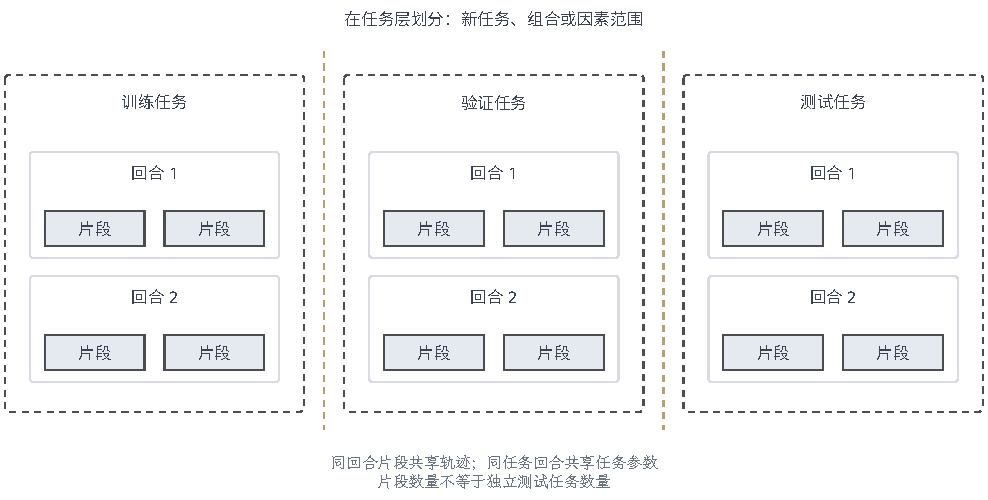
\includegraphics[width=167.238mm]{figures/10-reinforcement-learning/03-task-expansion-and-trustworthiness/tikz/rl-transfer-split.pdf}
 \caption{任务级划分与任务内采样。训练、验证、测试先按所声明的任务关系划分，再在每项任务内采集回合和片段；同色框中片段共享任务参数，不能按片段数声称独立任务数。图为抽样层级示意，不对应某批实际采集的任务或回合数量。}
 \label{fig:rl-transfer-split}
\end{figure*}

例如，三个独立生成的风向任务各采10回合，每回合切20段，共有600个片段，但任务层独立单位仍只有3个。这些是教学计数。若要评估任务平均回报的不确定性，应在任务层重采样，或用明确的分层统计模型；训练种子另是模型训练随机性的层级，不能将同一个训练种子下的600段当作600次独立训练。增加任务内完整回合主要改善已见任务中的回报估计，增加独立任务才增加关于任务总体的独立证据。一般的两层抽样界还要求固定完整学习或适应规则、在可见记录上定义有界评价损失，并核对任务独立、给定任务后的完整运行条件独立及候选选择方式；任意相邻RL片段不能直接满足这些条件。

测试协议应预先固定是否允许交互、奖励到达时刻、回合结束与任务切换的记忆重置，以及检查点数量。非平稳测试还要固定任务时间顺序；打乱时间后进行批量拟合，使用的是另一种历史读取与回合重排权限。不能让策略提前看到未来风向标签，也不能在恢复时间统计中删除失败回合。

泄漏不只来自重复轨迹。程序化生成器可能只更换纹理而复用同一路线模板，共享随机种子可能重现测试布局，目标描述可能直接包含最优动作编码。应检查生成器结构、种子谱系和描述字段。允许在一项测试任务内按既定协议适应，不等于允许根据整套测试成绩反复重设计训练方法；后一种选择应在验证任务上完成。

% Outline: 6.6.2
\subsection{在任务划分与固定预算下取得性能证据}
\label{sec:rl-transfer-evidence}

同一模型在新风向下先探测、再控制，探测期间的回报可能很低，适应完成后却能稳定到达终点。验证需要分别回答初始能做什么、学习期间付出多少代价、学完后能做什么。用$n$表示测试任务数，令$c_i$为第$i$个测试任务，$\pi_{i,0}$为尚未使用该任务的适应训练样本时的策略；$\pi_{i,B}$为按协议使用$B$步反馈后形成的策略。若使用前面的无限折扣任务，回报仍为未归一化$J_{c_i}$；若评价固定长度回合，则另注明时域、折扣和截断规则。

\term{零样本回报}为
$n^{-1}\sum_iJ_{c_i}(\pi_{i,0})$。\term{适应后回报}为
$n^{-1}\sum_iJ_{c_i}(\pi_{i,B})$，需要固定适应所得参数和任务后验或历史记忆、在独立评价回合上估计，并另报这部分交互数。评价时仍可按协议更新控制所需的物理状态估计，但不继续辨识任务；若一个记忆器无法分开这两项功能，就应明确评价中仍在适应。\term{预算内适应曲线}则记录随着累计目标交互增加，当前在线回合实际取得的回报，或在指定检查点另测的回报；这两种曲线不能混标，后者的查询成本也不能省略。

为评价学习期间的损失，固定同一目标任务、同一回合时域与初始分布，取指定比较策略$\pi_i^{\text{参照}}$。用$\pi_i^{(k)}$表示第$k$个适应回合的行为规则，区别于使用$B$步反馈后的$\pi_{i,B}$。在$M$个适应回合中定义
\begin{equation}
 \operatorname{AReg}_{i,M}
 =\sum_{k=0}^{M-1}
 \left[J_{c_i}(\pi_i^{\text{参照}})
       -J_{c_i}(\pi_i^{(k)})\right].
 \label{eq:rl-transfer-adaptation-regret}
\end{equation}
每个差额都以同一任务和回合条件下的参照回报为起点，求和得到学习期间相对该参照的累计损失。若比较者只是一条训练得到的策略，算法也可能超过它，使该量为负；名称不赋予参照者最优性，必须写出它可读取的任务标签、观测及模型字段。任务本身变化时，原来固定的$c_i$已不能代表所有回合，应另用式~\eqref{eq:rl-transfer-dynamic-regret}~及检测、恢复指标。

表~\ref{tab:rl-transfer-baselines}~给出比较协议。$B,K,L,C$分别表示目标适应步、梯度步、上下文长度和额外计算上限；它们是符号预算，不是某篇论文配置。共享训练的前期成本也应报告，即使目标任务比较只匹配部署预算。

\begin{table*}[t]
 \centering\small
 \begin{tabularx}{\linewidth}{@{}>{\raggedright\arraybackslash}p{23mm}*{3}{>{\raggedright\arraybackslash}X}@{}}
  \toprule
  比较对象 & 可用模型、任务描述与记录 & 目标预算 & 解释范围\\
  \midrule
  从头学习 & 随机初始化，不用源任务知识 & 相同$B,K,L,C$，独立评价另计 & 共享训练是否减少目标学习代价\\
  无适应 & 相同源模型，关闭任务更新 & 适应交互0、梯度0；执行预算相同 & 初始能力与适应带来的变化\\
  单任务训练 & 不共享参数的指定任务训练 & 报预训练量；目标比较仍匹配$B,K,L,C$ & 共享收益与容量、训练量差异\\
  已知任务身份 & 额外给真实任务参数 & 其余预算匹配，真实参数读取权限另标 & 知情参考；训练策略未必是上界\\
  可证明最优值 & 完整已知模型或允许额外读取真实状态或参数的可证明松弛 & 比较者权限显式列出 & 条件成立时才是性能上界\\
  \bottomrule
 \end{tabularx}
 \caption{性能证据需要的参照对象。“无适应”是刻意关闭反馈学习的消融，不能假装它花掉了与适应方法相同的学习预算；单任务参考若用目标任务交互记录预训练，必须披露这批额外目标任务训练样本。}
 \label{tab:rl-transfer-baselines}
\end{table*}

匹配预算以后，仍要区分平均水平与任务间差异。图~\ref{fig:rl-transfer-evaluation-curves}~用一组可复算的教学曲线说明汇总方法：设目标任务$i=1,\ldots,5$、训练种子$j=1,\ldots,3$，定义假设回报
\[
 \begin{aligned}
 y_{i,j}(B)&=0.2+0.7(1-e^{-B/30})+u_i e^{-B/60}+v_j,\\
 u_i&\in\{-0.16,-0.08,0,0.08,0.16\},\\
 v_j&\in\{-0.02,0,0.02\}.
 \end{aligned}
\]
式中共同项随预算$B$增加，$u_i$给出随适应减小的任务偏差，$v_j$给出训练种子偏差。所有数值都是作者设定的回报尺度，每条曲线是给定公式，不是实验测量。任务与种子均等权时，先对种子平均，再对任务平均；两组偏差分别和为0，得到均值$m(B)=0.2+0.7(1-e^{-B/30})$。阴影取种子平均后任务分数的均值加减一个样本标准差，即
$s_{\text{任务}}(B)=\sqrt{0.016}\,e^{-B/60}$，不是均值的置信区间。实际实验还需估计评价回合随机性，并说明任务与训练种子的嵌套或交叉方式。

\begin{figure}[htbp]
 \centering
 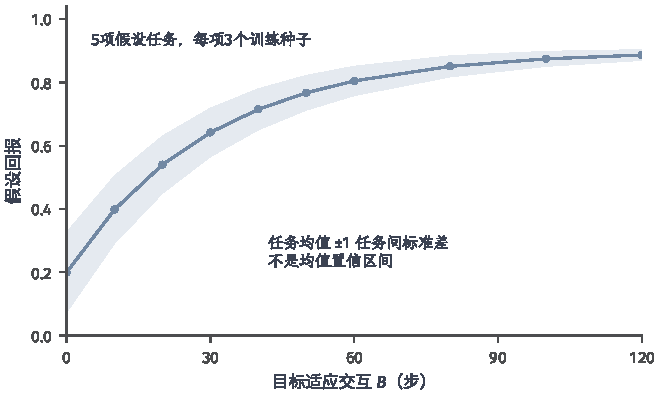
\includegraphics[width=112.000mm]{figures/10-reinforcement-learning/03-task-expansion-and-trustworthiness/matplotlib/rl-transfer-evaluation-curves.pdf}
 \caption{固定预算下均值与任务间离散程度的教学曲线。横轴为目标适应交互步数，纵轴为假设回报；线为5任务、3训练种子的等权均值，阴影为先平均种子后的任务均值$\pm1$样本标准差。图源按正文公式在所列检查点计算并线性连接，无算法实测排名；真实协议中的评价交互还须单独计入。}
 \label{fig:rl-transfer-evaluation-curves}
\end{figure}

不同任务的回报尺度不同时，可以分别报告原始分数，或使用预先固定、具有解释意义的参照范围归一化；归一化分母接近0的任务需要单独处理。不能观察测试结果后选择有利的缩放方法。汇总还应报告各任务组的失败比例、差异幅度及不确定性，避免少数高分任务掩盖多数任务无收益。训练得到的知情策略即使表现很好，也只有参考意义，不能未经证明称为最优上界。

% Outline: 6.6.3
\subsection{从迁移结果到共享假设的诊断与修正}
\label{sec:rl-transfer-diagnosis}

共享模型比从头学习模型多得了回报，首先说明在某个任务组和预算下出现了差别，还没有说明差别能否稳定重复、由什么造成。相对于明确的不共享或从头学习基线，在相同目标描述、可见反馈与预算下，以回报增加表示\term{正迁移}（positive transfer），以回报降低表示\term{负迁移}（negative transfer）；若改用损失或累计差额，改善方向也须相应改变。正负依赖任务组、指标和预算：学习早期有益、最终性能稍低，可以同时成立。因此一次更高的样本均值还不足以支持稳定的正迁移结论。

考虑四项等权教学任务，基线回报均为$0.6$，共享模型回报分别为$0.8,0.8,0.8,0.2$。共享均值为$0.65$，平均提高$0.05$，第四项任务却下降$0.4$。若第四项恰好使用未覆盖的左风，这一结果提示检查任务分层与覆盖；它本身尚不能证明动力学共享假设错误。

诊断需要补充可以区分解释的证据。训练任务或状态动作访问覆盖不足时，应控制任务采样和相关状态动作访问；表示容量不足时，应比较参数量和计算量匹配的模型，并检查目标位置、任务提示等关键观测差别是否被抹去；优化冲突时，可比较分任务梯度的内积、独立训练与任务权重调整。负梯度内积只是局部冲突信号，不自动说明两个任务在真实结构上不兼容。要检验共享结构，可保持其余训练条件，替换被怀疑的共同模块为任务条件或独立模块，并在受影响任务组上重新评价。

图~\ref{fig:rl-transfer-diagnosis}~将修订对象分开。匹配容量后仅改变任务权重便恢复性能，更支持训练机制解释；在充分覆盖与多种优化设置下，共享转移模块仍系统性地把相反风向混合，而任务条件模块消除了相应预测误差，才为重新检查共享假设提供较直接的证据。

\begin{figure*}[htbp]
 \centering
 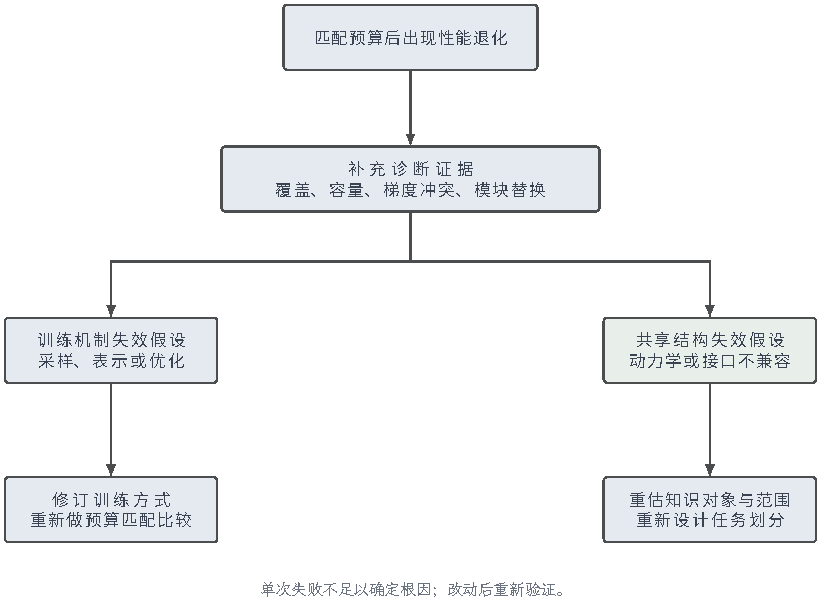
\includegraphics[width=139.019mm]{figures/10-reinforcement-learning/03-task-expansion-and-trustworthiness/tikz/rl-transfer-diagnosis.pdf}
 \caption{由退化结果形成可区分的诊断。分支表示待检验解释，不能只凭一次失败直接确定根因；训练问题修订采样、容量或优化，结构问题则重估共享对象及适用任务。图为本章诊断关系的原创示意。}
 \label{fig:rl-transfer-diagnosis}
\end{figure*}

单一基线可能容量不足，一次种子可能恰好失败，模块替换也可能同时增加容量。因此需要逐项控制差异，报告重复试验与不确定性，而不是见到改进就倒推唯一原因。共享结构一旦改变，原来的任务支持与组合假设也要重查，不能沿用旧条件下的泛化声明。

% Outline: 6.6.4
\subsection{由评测证据限定泛化与适应声明}
\label{sec:rl-transfer-claims}

同是“在新任务上成功”，支持内新终点上的直接执行，与无预告变风后的在线恢复，需要的证据不同。迁移声明应同时给出目标任务关系、可读取的任务描述与交互记录、适应预算和性能证据，才能让读者重建实际测试的问题。表~\ref{tab:rl-transfer-claims}~汇总本章导航变体分别能够支持的说法；这些结论以相应实验确实取得可靠证据为前提，本章教学数值本身不构成算法实验证据。

\begin{table*}[t]
 \centering\small
 \begin{tabularx}{\linewidth}{@{}>{\raggedright\arraybackslash}p{22mm}*{4}{>{\raggedright\arraybackslash}X}@{}}
  \toprule
  目标任务关系 & 可读任务描述与反馈 & 适应预算 & 评价证据 & 允许的结论\\
  \midrule
  支持内新目标 & 兼容的目标坐标 & 无反馈适应 & 任务级留出零样本回报 & 声明总体内的描述条件泛化\\
  未见目标与风组合 & 相同描述字段 & 固定$B,K,L,C$ & 留出联合组合的分组结果 & 指定因素与组合上的能力\\
  未见噪声范围 & 描述或获准历史 & 明确探测与更新 & 范围外分组、失败与误差 & 已测范围内的外推证据\\
  固定隐藏风向 & 无真实风标签，反馈逐步可见 & 探测、恢复、评价均计 & 辨识误差、适应回报与参照差额 & 规定描述与反馈条件下的固定任务适应\\
  变化风向序列 & 不提前见未来变化 & 按时间顺序持续交互 & 动态遗憾、检测延迟与恢复 & 指定变化预算及信号下的跟踪\\
  \bottomrule
 \end{tabularx}
 \caption{证据与声明的对应关系。支持内、组合、范围外、固定隐藏任务和变化任务不是逐级自动推出的能力；每一行都需要自身的任务划分与协议。}
 \label{tab:rl-transfer-claims}
\end{table*}

训练任务数量很大，但每项只改变同一地图的颜色时，测试高分仍不能证明新几何泛化。目标和风向都单独测过，但从未共同改变时，不能推断组合有效。若变化检测器提前读到了下一回合任务标签，快速恢复也不能支持无预告持续适应。这些反例没有否认已测分数，而是限定分数回答的问题。

还应区分平均能力与最低要求。对声明任务分布取得较高平均回报，不等于在所有允许扰动下都不低于某个阈值；后者需要明确扰动集合、风险或最坏情形准则，以及相应验证。鲁棒性与可信保证留到第~\ref{chap:rl-trustworthy}~章讨论，不能由本章经验泛化结果直接推出。

% Outline: 6.7
\section{本章小结}
\label{sec:rl-transfer-summary}

回到章首的小车：共同终止规则下换奖励目标，可以保留移动模型，却要按新奖励重算价值；若换终点还改变吸收规则，就连完整转移核也需要重查。地面变滑时，目标含义可以保留，旧后果预测却可能失效。能否迁移取决于复用对象所需的共享条件，以及新任务是否满足这些条件。参数形状相同、平均回报相近或任务编号相邻，都不能替代逐项检查。

训练得到的表示、模型、价值、策略初始化和技能，在部署中仍要结合描述、历史与权限，才能形成具体策略。固定参数可以通过记忆适应，参数更新需要获准且能支持目标估计的训练样本，持续交互只有在反馈有区分力且动作获准时，才可能取得区分候选任务所缺的观测或奖励。后继特征把共同动力学下的后果与奖励权重分开，GPI逐状态组合已有策略的候选动作；它们没有消除奖励类和策略覆盖的限制。贝叶斯任务更新则说明怎样用正确似然认识固定任务，不能直接累积过时证据来跟踪变化任务。

认识固定未知任务与追踪变化任务并不相同。每轮独立变化的两臂例子表明，计算或记忆无法补出缺失的当前最优臂提示。任务级划分、完整预算、匹配比较者和分层失败诊断，共同约束泛化与适应声明。伙伴与对手也会带来任务变化，但各自的目标与共同学习需要联合建模。第~\ref{chap:rl-multi-agent}~章将考察这些依赖，并把任务描述、反馈读取范围与适应预算的约定用于交互双方。

\chapter{多智能体协作和博弈}
\label{chap:rl-multi-agent}

前几章始终只有一个决策者，环境在它眼里是一套固定的物理规则。本章放宽这一前提：环境中同时存在多个会决策、而且可能也在学习的参与者。先看一个最日常的例子：两个人从窄通道的两端相向而行。同样是向前迈步，对方愿意等待时我就能通过，对方也往前冲时两人就可能堵在入口。也就是说，同一个动作的后果不仅取决于通道的物理规则，还取决于另一个人的选择；若对方也在学着避让，那么今天还奏效的策略，明天可能就不再管用。多智能体问题的本质，就是行动后果由所有人的选择共同决定，而各方的选择又可能随交互不断改变。

要在这种交互中套用价值学习，必须先想清楚三件事：要最大化的是谁的回报？每个人行动前能读到哪些观测、历史和消息？对方的策略会不会随交互而变化？这三者缺一不可。多方交互仍使用第\ref{chap:rl-overview}章已说明的策略、回报与价值，以及第\ref{chap:rl-learning}章的采样和更新工具，只是对象之间多了层层依赖：收益关系决定“怎样的行为才算好”，观测与消息的读取权限决定哪些策略真正能执行，联合经验用于估计行为后果，而策略一旦更新，又反过来改变下一批经验的来源。本章大致顺着这条依赖链展开——先搭共同设定、再按收益关系确定行为标准，然后讨论经验怎么采、后果怎么估、策略怎样一起更新，最后处理参与者变化以及如何评价与验证。估计后果时，可以同时保留双方动作、比较自身替代动作的后果，或直接预测伙伴会怎样行动；更新策略时可以沿收益梯度改进，也可以用历史策略来安排训练配对和响应对象。这些选择处理的是不同层面的依赖，并不互斥，可以组合使用。图\ref{fig:rl-multi-agent-map}画出这些依赖。

\begin{figure}[htbp]
  \centering
  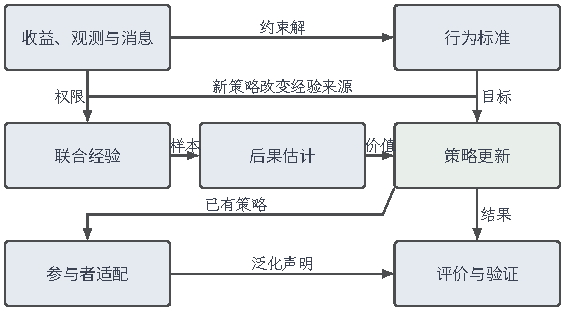
\includegraphics[width=95.652mm]{figures/10-reinforcement-learning/03-task-expansion-and-trustworthiness/tikz/rl-multi-agent-map.pdf}
  \caption{多智能体求解中的问题关系。实线连接约束、交互记录与后果估计的用途，外侧回路表示策略更新改变后续经验来源；底部的适配与评价检查行为标准在所声明参与者范围内是否成立。}
  \label{fig:rl-multi-agent-map}
\end{figure}

% Outline: 7.1
\section{收益、信息与参与者的共同设定}
\label{sec:rl-multi-agent-setting}

% Outline: 7.1.1
\subsection{用联合动作、转移与个体回报定义决策过程}
\label{sec:rl-multi-agent-process}

把通道截成一次“谁先通过”的竞争，可以得到一个确定性的教学任务。初态为两人都尚未通过的$s_{\text{入口}}$，另有“1先通过”“2先通过”和“碰撞”三个终止状态；两人都能观察当前状态，并读取自己的奖励。在入口，各人选择前进$F$或等待$W$。联合动作$(F,W)$使1先通过，两人的奖励依次为$(-1,-2)$；$(W,F)$使2先通过，奖励为$(-2,-1)$。$(F,F)$导致碰撞，双方各得$-4$并终止；$(W,W)$使系统留在入口，双方各得$-1$，下一步重新选择。三个终止状态都吸收，后续奖励为0。这里的数值是独立教学设定，不取自前几章的随机网格。

这个小任务把多人问题新增的依赖具体化：推动状态变化的是联合动作，每个人的奖励可以不同，观察权限也须逐人规定。一般环境还可能让奖励、后继观测和终止标记共同随机产生，因此需要一个联合生成模型。

\begin{definition}[多参与者序贯决策]
\label{def:rl-multi-agent-game}
给定正整数$m$、非空状态空间$S$、各人的非空行动空间$\mathsf A_i$与非空观测空间$\mathsf O_i$，均配备可测结构。设参与者集合为$\mathcal N=\{1,\ldots,m\}$，用$-i$表示除$i$之外的参与者，$\mathsf A_i(s)$为$i$在状态$s$中的非空合法动作集合，合法状态—联合动作对构成可测集合。各人动作组成$\bm a=(a_1,\ldots,a_m)\in\prod_i\mathsf A_i(s)$。以下各核与策略均可测，允许的合法策略集合非空。环境以从合法状态—联合动作对到$S\times\mathbb R^m\times\prod_i\mathsf O_i\times\{0,1\}$上概率测度的联合反馈核
\[
 K(\mathrm ds',\mathrm d\bm r,\mathrm d\bm o',\mathrm dd\mid s,\bm a)
\]
一次生成后继状态$s'$、个体奖励向量$\bm r=(r_1,\ldots,r_m)$、下一联合观测$\bm o'$及终止标记$d\in\{0,1\}$。共同转移核和期望奖励分别是这一联合律的边缘与条件均值：
\[
 \begin{aligned}
 T(B\mid s,\bm a)
 &=K\!\left(B\times\mathbb R^m\times\prod_i\mathsf O_i
              \times\{0,1\}\mid s,\bm a\right),\\
 R_i(s,\bm a)
 &=\int r_i\,K(\mathrm ds',\mathrm d\bm r,\mathrm d\bm o',\mathrm dd\mid s,\bm a).
 \end{aligned}
\]
其中$B$是$S$的可测子集，并要求各合法$(s,\bm a)$下$\int|r_i|\,\mathrm dK<\infty$。有限或可数空间中的积分按相应点质量求和。这里没有假设奖励、观测、后继状态和终止标记条件独立；若要使用因子化接口，须另行给出因子分解。

行动权限由局部历史$I_{i,t}$限定：它只包含$i$在动作$t$之前获准取得的观测、自身过去动作、可见奖励和已收到的消息。执行第$t$步联合动作后，联合反馈核先产生反馈，各人只能把协议允许其看见的部分写入$I_{i,t+1}$；策略产生的消息及其送达时刻另由通信协议规定。策略$\pi_i(a_i\mid I_i)$只依据该参与者获准取得的局部观测、消息和自身行动记录选择动作。记各人的策略合称为$\bm\pi$。初始分布$\mu_0$专指物理初态分布；下式的期望还固定初始观测、初始消息与公共信号的生成约定。要求每个参与者的折扣奖励和绝对可积，即$\mathbb E\sum_{t\geq0}\gamma^t|r_{i,t}|<\infty$；有界逐步奖励是充分条件。参与者$i$要评价的未归一化折扣回报为
\[
 J_i(\bm\pi)=\mathbb E_{\mu_0,\bm\pi}
 \left[\sum_{t=0}^{\infty}\gamma^t r_{i,t}\right],
 \qquad 0\leq\gamma<1.
\]
\end{definition}

把所有人的策略合在一起称为联合策略$\bm\pi$。它能不能写成各人策略的乘积，取决于动作是怎样产生的：给定联合历史$\bm I$后，若各人独立地各自随机化，才有$\bm\pi(\bm a\mid\bm I)=\prod_i\pi_i(a_i\mid I_i)$；若行动前先广播过一个公共随机信号$c$（比如抽签决定谁先走），那么这种独立性只能在给定$c$之后使用。把信号平均掉，得到$\sum_c p(c\mid\bm I)\prod_i\pi_i(a_i\mid I_i,c)$，一般不能再拆成各自边缘分布的乘积。若所有人都只行动一次，可以把每组联合动作的收益排成一张矩阵，得到矩阵博弈：每个格子对应一个联合动作，格子里写各方收益。加入共同状态和转移后，就相当于“在每个状态上各摆一局矩阵博弈，而这一局的动作结果又决定下一局发生在哪个状态”，这称为随机博弈（stochastic game），Shapley 建立了其完全可观测形式的经典理论\scite{rl1-shapley1953-games}。

一个自然的简化念头：既然真正要优化的只是我自己的策略，能不能把其余人也当成“环境”的一部分，继续套用单人 MDP？答案是有条件的——当其他人都使用固定的状态条件策略、并且给定$s$后他们的联合动作与我的动作独立随机化时，可以把他们各种动作出现的概率当作随机转移的一部分，按概率把转移与奖励加权平均掉。这一步边缘化给出$i$实际面对的过程：
\begin{align}
 T_i^{\bm\pi_{-i}}(s'\mid s,a_i)
 &=\sum_{\bm a_{-i}}\bm\pi_{-i}(\bm a_{-i}\mid s)
 T(s'\mid s,a_i,\bm a_{-i}),\label{eq:rl-multi-agent-induced}\\
 R_i^{\bm\pi_{-i}}(s,a_i)
 &=\sum_{\bm a_{-i}}\bm\pi_{-i}(\bm a_{-i}\mid s)
 R_i(s,a_i,\bm a_{-i}).\nonumber
\end{align}
在通道中，对方以概率$q$等待时，自己前进的通过概率为$q$，期望即时收益为$q(-1)+(1-q)(-4)=-4+3q$。若对方学习后把$q$从$0.8$降到$0.2$，这两个量都会改变，尽管共同的$T$和$R_i$没有变化。因而，对$i$而言过程不再平稳，可能仅仅是因为边缘化时使用的对方策略变了，而非物理环境发生漂移。

使用式\eqref{eq:rl-multi-agent-induced}时，要检查的是$\mathbb P(\bm a_{-i}\mid s,a_i)=\bm\pi_{-i}(\bm a_{-i}\mid s)$，而不是要求其他人彼此独立。公共信号若使双方动作相关，观察到自身动作也可能改变对其他动作的判断，不能直接用其边缘分布加权；应先把信号纳入条件，再检查等式。另一个限制来自记忆：对方若按过去碰撞次数调整让行概率，当前位置就不足以预测其下一动作。需要把相关记忆或类型纳入充分状态，或者在历史上定义过程，才能讨论相应的评价与收敛；原有平稳MDP结论不能直接沿用。

% Outline: 7.1.2
\subsection{不同收益关系下的合作、零和与一般和问题}
\label{sec:rl-multi-agent-payoffs}

保留入口和两种动作，改变奖励就会改变要解决的问题。若两人共享奖励，可另设碰撞$-2$、都等待$-1$、恰好一人前进$2$，目标是共同避免冲突并尽快通行。若只比较谁先通过，可让$(F,W)$给第一人$1$，$(W,F)$给第一人$-1$，其余为$0$，第二人取相反收益。若各人承担自己的时间成本，则等待者可能比先行者损失更多，而碰撞同时损害双方。以上是分别说明三种收益关系的教学设定，不是同一奖励表。

这三种奖励安排恰好对应多智能体中三类典型的收益关系，也是后面判断“策略是否变好”的三种不同标准。\term{完全合作}（fully cooperative）意味着所有人评价的是同一个回报目标，相当于同一支队伍：把蛋糕做大对每个人都有利。\term{两人零和}（two-player zero-sum）要求每个结果满足$r_{1,t}+r_{2,t}=0$，即一方的每一分收益恰好是另一方的损失；对整条轨迹求和取期望便有$J_2=-J_1$，最典型的就是零和对抗。\term{一般和}（general-sum）则不限制各收益之间的关系，可以同时含有共同利益与个人冲突——通道里双方都不希望碰撞，却又都想先通过。还要特别强调：目标相同不代表两人能读到相同的观测与消息，更不保证两个各自独立学习的人能自发形成彼此兼容的让行约定。表\ref{tab:rl-multi-agent-payoffs}据收益关系列出对应的行为标准，使后续“改进”有明确的比较对象。

\begin{table}[htbp]
 \centering
 \begin{tabularx}{\linewidth}{@{}l >{\raggedright\arraybackslash}X >{\raggedright\arraybackslash}X@{}}
 \toprule
 收益关系 & 标准与单方偏离 & 额外社会选择\\
 \midrule
 完全合作 & 在允许的局部观测与消息条件下最大化共同$J$；单方改动也按共同收益计 & 若存在多个最优策略，仍需选择兼容约定\\
 两人零和 & 最大化最坏收益；偏离检验可被利用的程度 & 价值标准已给定，风险限制可另设\\
 一般和 & 各自偏离是否获利；可另优化福利 & 必须另定福利、公平及取舍\\
 \bottomrule
 \end{tabularx}
 \caption{同一任务接口在不同收益关系下的行为标准。完全合作可比较共同回报，零和可比较最坏收益，一般和须另行指定社会目标。}
 \label{tab:rl-multi-agent-payoffs}
\end{table}

一般和中，总收益与个人激励可能冲突。总收益很高的结果可能诱使一人立即偏离；没有人愿意单方偏离的结果也可能使双方收益都很低。奖励求和可以定义一种福利指标，却既不规定收益如何分配，也不保证个人愿意维持该结果。评价时必须把福利、分配和稳定性分别说明。

% Outline: 7.1.3
\subsection{不同行动、观测与通信时序下的信息结构}
\label{sec:rl-multi-agent-information}

收益关系确定之后，还要确定作出选择时知道什么。通道中的“我先走”若在对方行动前送达，可以支持本轮避让；若延迟一轮，只能进入$I_{i,t+1}$。图\ref{fig:rl-multi-agent-timing}为此分别标出观测、发信、收信、行动和反馈。训练日志事后收齐消息，不意味着动作$t$可以使用它。行动本身也有时序限制：顺序行动的后手可能观察先手动作，同时行动的双方则不能据本轮尚未提交的对方动作决策。

\Needspace{16\baselineskip}
实现时，依次调用程序不等于允许依次观察行动。PettingZoo以统一接口支持多类多智能体环境，其中智能体—环境循环（agent environment cycle, AEC）接口逐个调用参与者。用它实现同时行动任务时，仍要屏蔽本轮其他人尚未共同提交的动作，否则调用顺序就意外地让后手提前读到了本轮其他人的动作\scite{rl7-terry2021}

\begin{figure}[htbp]
 \centering
 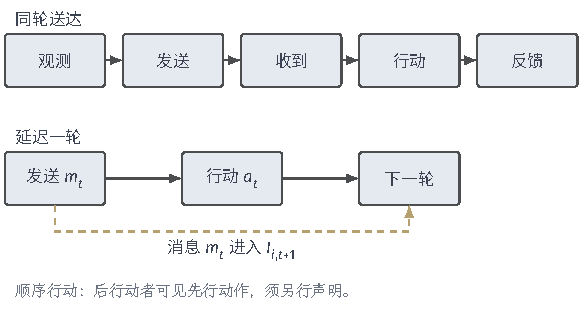
\includegraphics[width=98.616mm]{figures/10-reinforcement-learning/03-task-expansion-and-trustworthiness/tikz/rl-multi-agent-timing.pdf}
 \caption{消息何时进入策略输入。实线表示本轮可读取的观测与已送达消息，虚线表示下一轮才送达的消息；顺序行动还可能允许后手观察先行动作，这一权限不属于同时行动。}
 \label{fig:rl-multi-agent-timing}
\end{figure}

确定送达时刻后，还须规定消息携带什么。通信模型CommNet让参与者发送连续向量，把同伴发送的消息聚合成一个表示，再将其用于协作决策。这些表示能成为本轮策略输入的前提仍是动作前按协议送达，网络中的聚合运算不能替代实际通信权限\scite{rl7-sukhbaatar2016}

前面的讨论默认每个人都能看到完整状态，但真实场景往往不是这样：过道里看不到拐角后面是否有人，扑克玩家也看不到对手的底牌。于是需要给每个参与者单独规定他能看到的观测，而不是假设大家共享同一个$s$；各人看到不同信号的随机博弈称为\term{部分可观测随机博弈}（partially observable stochastic game, POSG）。把定义\ref{def:rl-multi-agent-game}中“下一观测”的条件单独取出，常将定义\ref{def:rl-multi-agent-game}中的观测条件边缘记为联合观测核$K_o(\bm o'\mid s',\bm a)$，并另给初始观测分布，说明状态怎样生成每个人看到的信号。采用这一简化接口，意味着观测边缘在给定$(s',\bm a)$后不再依赖旧状态；它不表示观测与奖励或终止反馈条件独立，完整耦合关系仍由$K$规定。局部观测$o_i$不等于完整状态$s$。若进一步共享团队奖励、并要求各策略只使用自己的历史，就得到\term{分散部分可观测马尔可夫决策过程}（decentralized POMDP, Dec-POMDP）：大家为同一个回报行动，却分别依据各自的观测、动作、奖励历史与合法消息作出选择。这里的困难超出单人 POMDP：即使把各人的观测合起来足以恢复状态，每个人在决策时也没有权限读取别人的观测。通信可以表示为动作的一部分或单独的消息阶段，顺序行动可以在状态中标记当前行动者；这些建模方式都必须保留实际观测范围和消息送达时序的限制\scite{rl7-bernstein2002}。

局部观测和可读行动历史对策略的限制可以用一个有限隐藏牌面游戏说明。这不是标准扑克；以下规则定义了全部随机性与收益。机会方以各$1/2$的概率给参与者1发高牌$H$或低牌$L$，只有1看见牌，两人先各投入一单位。1先选择下注$B$或过牌$K$：下注后由2选择弃牌$F$或跟注$C$；过牌后由2选择过牌$K$或下注$B$。若2也过牌，立即摊牌；若2下注，1再选弃牌$F$或跟注$C$，随后结束。摊牌时，高牌由1赢，低牌由2赢；无人加注时胜者净得$1$，跟注后胜者净得$2$。有人弃牌时，未弃牌者净得$1$。另一人取相反净收益，全局只有终局收益，不设折扣。

图\ref{fig:rl-multi-agent-card-tree}把这些规则展开成完整历史树：顶部机会节点生成牌面，圆节点表示决策，叶节点给出1的净收益。面对1首次下注，2不能区分高牌与低牌分支上的两个节点，因而它们属于同一\term{信息集}（information set），即依据该参与者已取得的观测、动作、奖励和消息无法区分的一组完整历史。2必须在两处使用相同的跟注概率；按牌面分别设概率就使用了参与者2并未看到的牌面。相反，2能够看见1是下注还是过牌，这两种情形必须属于不同的信息集。

\begin{figure}[htbp]
 \centering
 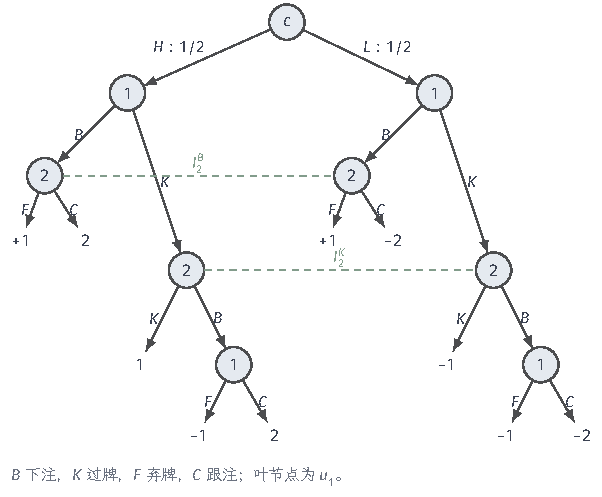
\includegraphics[width=101.946mm]{figures/10-reinforcement-learning/03-task-expansion-and-trustworthiness/tikz/rl-multi-agent-card-tree.pdf}
 \caption{隐藏牌面教学游戏的完整历史树。虚线各自连接2面对下注、面对过牌时不能区分的节点；1知道牌面，其节点不跨牌面合并。叶节点标1的净收益，2取相反数。}
 \label{fig:rl-multi-agent-card-tree}
\end{figure}

这里引入的\term{信息集}（information set），直观上就是“在某个参与者看来无法区分的一组完整局面”：处在同一信息集的节点，对他而言可能给出完全相同的观察和历史，所以他必须在这些节点上使用同一套动作概率。但信息集也不能抹掉参与者自己的记忆。\term{完全回忆}（perfect recall）要求同一信息集里的所有历史，都具有相同的“自己过去知道过什么、做过什么”序列。

% Outline: 7.1.4
\subsection{信息权限与联合策略表示}
\label{sec:rl-multi-agent-permissions}

若由一个能取得全局状态与各人历史的控制器选择联合动作，就可以集中决策。困难在于训练与部署可读取的变量不同：训练通常在仿真器或服务器上进行，可以记录全局状态、联合动作和各人的历史；真实部署时，每个人却只有局部传感器，不能即时读取其他人的位置、局部观测与历史，通信也可能受限。这些集中变量可以帮助训练评论家，但执行策略仍不能依赖部署时读不到的变量。\term{集中训练、分散执行}（centralized training with decentralized execution, CTDE）正是把这两种权限分开：训练时允许用全局状态、联合动作或其他人的历史来估计价值，行动策略在部署时则只能读取本地历史及获准送达的消息。

\begin{figure*}[htbp]
 \centering
 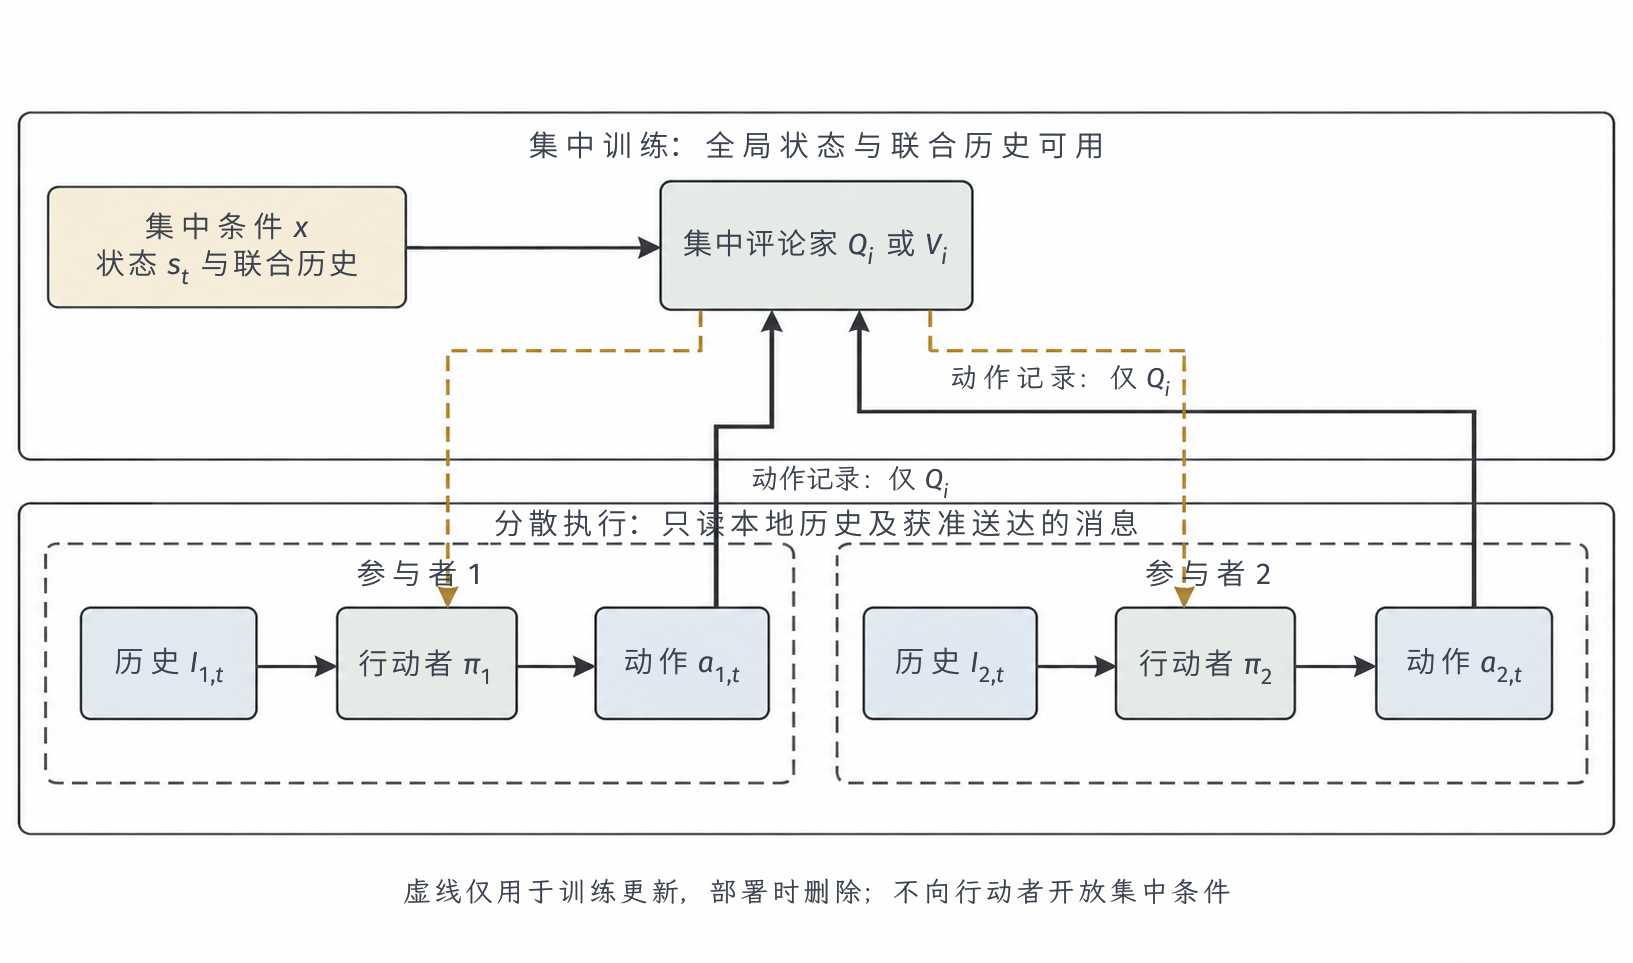
\includegraphics[width=157.400mm]{figures/10-reinforcement-learning/03-task-expansion-and-trustworthiness/generated/rl-multi-agent-ctde/figure.png}
 \caption{CTDE中的集中训练与分散执行。上区的集中评论家可使用全局状态及联合历史，下区各行动者只使用本地历史和获准消息。向评论家上送的当前动作仅用于$Q_i$，估计$V_i$时不取当前动作作为条件；部署时删除训练虚线，也不向行动者开放集中条件。两个参与者仅为示例。}
 \label{fig:rl-multi-agent-ctde}
\end{figure*}

在执行权限相同的前提下，还可以选择是否共享参数。若两人的观测、动作和角色含义兼容，共享$\pi_{\bm\theta}(a_i\mid I_i)$可让同一函数服务两人，但不会让他们读取对方的局部观测或消息。加入身份编码$e_i$后，网络可按编号形成“1先走、2等待”的约定；身份重排却可能使该约定失效。独立参数容纳不同动作接口或角色，但需分别存储和拟合各人的网络，并寻找能彼此配合的策略组合。参数量和训练样本需求还取决于网络结构与任务，不能仅由参数独立就断言样本成本更高。身份是否必要，应由任务中的角色含义决定。

通信也可以参与参数学习。可微智能体间学习（differentiable inter-agent learning, DIAL）在训练时通过可微信道传递梯度，使发送者得到关于消息用途的反馈，部署时则改用受限的离散消息。连续训练近似与实际离散信道并不相同，量化可能改变接收到的消息内容，因此仍要检查部署消息能否支持学到的协调行为\scite{rl7-foerster2016}

要检查这种训练与执行差异，协议必须说明谁向谁发送什么、何时送达，以及花费多少带宽。表\ref{tab:rl-multi-agent-communication}比较四种可与CTDE组合的接口。能否通过消息反向传播属于训练计算条件，链路延迟、带宽和接收权限则约束实际执行，两者不能相互替代。

\begin{table}[htbp]
 \centering
 \begin{tabularx}{\linewidth}{@{}l >{\raggedright\arraybackslash}X >{\raggedright\arraybackslash}X@{}}
 \toprule
 接口 & 发送者、接收者与内容 & 时序、带宽及训练／执行条件\\
 \midrule
 固定协议 & 每人向指定邻居发角色或让行码 & 动作前收信；固定比特数；两阶段协议均保持\\
 可微通信 & 所有人向聚合器或同伴发实向量 & 每轮一至多次交换；向量维数固定；执行须保留信道\\
 离散消息 & 每人向获准接收者发有限字母表符号 & 训练可用连续松弛；执行量化后重新核验\\
 图消息传递 & 节点向图邻居发嵌入或定向消息 & 边数与轮数决定带宽；部署只能使用可发现的边\\
 \bottomrule
 \end{tabularx}
 \caption{四种消息接口的执行条件。比较时须同时说明发送者与接收者、消息内容、送达时刻及通信成本，而不只报告训练中是否可微。}
 \label{tab:rl-multi-agent-communication}
\end{table}

若并非所有人都需要同一条消息，可以进一步学习发送对象。定向多智能体通信（targeted multi-agent communication, TarMAC）用定向寻址计算接收权重，让不同接收者聚合不同内容。它解决的是“消息给谁”，可以与消息内容的表示、训练信道的选择共同使用，但仍须符合部署的接收权限\scite{rl7-das2019}

% Outline: 7.1.5
\subsection{不同数据访问与参与者变化方式下的学习问题}
\label{sec:rl-multi-agent-access}

相同的两人通道，还会因交互记录的采集、访问权限和对方变化方式而形成不同学习问题。对方遵守固定避让规则时，学习者可以探索其响应；双方共同训练时，刚估计的规则下一轮可能已改变；从历史策略库抽样时，每场经验还取决于抽到了哪个版本。表\ref{tab:rl-multi-agent-access}将参与者条件与记录访问权限交叉列出。其中“可改变”只指学习者按协议能控制的因素，第三方主动改变策略不属于学习者的采集权限。

\begin{table}[htbp]
 \centering
 \begin{tabularx}{\linewidth}{@{}l >{\raggedright\arraybackslash}X >{\raggedright\arraybackslash}X >{\raggedright\arraybackslash}X@{}}
 \toprule
 参与者条件 & 在线访问 & 固定联合日志 & 有限批次访问\\
 \midrule
 固定伙伴 & 可改自身行为，伙伴不变 & 不可重采；还原固定版本 & 批间改自身，批内固定\\
 同步学习者 & 可按约定更新双方 & 仅观察历史更新，不能重放新响应 & 批间同步更新，批内冻结\\
 群体抽样 & 可改获准的抽样分布 & 只能使用已记录群体支持 & 批间改抽样，批内固定\\
 主动适应者 & 自身动作可诱发其响应，未必可控 & 响应机制可能不可识别 & 须声明对方是否随批内历史更新\\
 \bottomrule
 \end{tabularx}
 \caption{记录访问权限和参与者变化共同限定可做的采集。有限批次若包含对方的批内适应，整批就不能被描述为固定联合策略产生的交互记录。}
 \label{tab:rl-multi-agent-access}
\end{table}

多智能体建模不要求所有参与者都在学习：即使只优化一个策略，也须表示其他行为怎样共同决定结果。反过来，同时运行多个固定规则代理或多个语言模型角色，并不能说明发生了强化学习。还需给出被优化的策略、交互产生的反馈和更新所针对的回报。“多人对话”描述的是交互形式，不能代替这些学习条件。

% Outline: 7.2
\section{不同收益关系下的行为标准}
\label{sec:rl-multi-agent-solutions}

模型建好了，但“回报提高”在不同收益关系下含义完全不同：合作时是共同蛋糕变大，零和时是最坏情况下不吃亏，一般和时则要问有没有人愿意单方面改变行为。因此在讨论学习之前，必须先选定衡量行为的标准。下面保留有限两动作的教学接口，分别考察共同目标下的团队最优、零和对抗中的最坏情形价值、以及一般和博弈中的单方偏离稳定性。三者对应的收益关系不同，不能把其中一种意义上的“改进”当成另一种标准也得到了满足。

% Outline: 7.2.1
\subsection{共同目标下的联合最优标准}
\label{sec:rl-multi-agent-team}

共享回报时，目标函数很直接：最大化共同的$J(\bm\pi)$。但这里有一个初学者极易忽略的限制——可搜索的策略范围只能是部署时真正可执行的$\Pi_{\text{分散}}$，其中每条策略都必须满足局部观测范围、消息时序和公共随机性的约束。训练服务器可以用全局状态或联合历史来帮助估计、帮助求解，却不能因此让部署时的行动者直接读到这些变量。一个能看到全局的“中央大脑”当然可能做得更好，下面的包含关系就给出这种集中求解相对分散最优值的上界。

\begin{theorem}[集中与分散策略的可行集合]
\label{thm:rl-multi-agent-inclusion}
设奖励有界且$0\leq\gamma<1$。若集中控制器在每个决策时刻取得分散系统的全部可用历史，还能模拟其私有随机性、公共随机性和合法通信，就能为每个分散策略生成相同的轨迹分布。按所实现的分布识别策略，有
\[
 \Pi_{\text{分散}}\subseteq\Pi_{\text{集中}},
 \qquad
 \sup_{\bm\pi\in\Pi_{\text{分散}}}J(\bm\pi)
 \leq
 \sup_{\pi\in\Pi_{\text{集中}}}J(\pi).
\]
\end{theorem}
\begin{proof}
对任意分散策略$\bm\pi$，让集中控制器分别保存各人的局部历史，并在每一时刻按原协议产生公共信号、私有随机数和消息，再调用各$\pi_i$生成联合动作。这样既不改变随机机制，也不向局部策略额外提供其他人的观测或消息。模拟从相同的初始历史分布开始；若直到$t$的联合历史分布相同，相同策略调用就产生相同的条件动作分布，未变的联合反馈核和合法消息生成、送达协议继而产生相同的$t+1$历史分布。这里的反馈包括各人可见的奖励、观测与终止标记，不能只比较状态边缘。归纳可得所有有限轨迹分布一致。有界奖励与$\gamma<1$保证相应折扣回报期望一致，所以每个分散系统可达的回报都能由集中控制器实现。对两种可达集合取上确界，便得到不等式；若有限问题中最优策略存在，上确界可写成最大值。
\end{proof}

集中上界不一定能分散实现。设通行前产生均匀二值信号$c\in\{0,1\}$，两个值的概率各为$1/2$，只有两人都选$c$时团队得$1$，否则得$0$。集中控制器看到$c$，每次都能得$1$。对分散双方，假设各自观测均与$c$独立，不许互传观测，使用的随机数也独立于$c$及双方观测。允许公共随机数只能帮助两人协调，不能让任一人知道$c$；其动作仍与$c$独立。成功事件包含在第一人选对的事件中，故
\[
 \mathbb P(a_1=a_2=c)\leq\mathbb P(a_1=c)=\frac12.
\]
这里仅使用每个人动作与$c$的独立性，没有把逐个独立扩大为联合观测或联合动作的独立性。固定都选0可以达到$1/2$这一上界。若允许在行动前广播$c$，局部策略才有条件按信号选择，分散最优值也才恢复为1。

因此，声称团队最优时须同时给出回报目标和允许的观测、历史与消息条件。一次成功协调仅说明找到了一个有效行为，参数空间的局部最优也不等于整个可行策略集合的最优。若原问题的个人收益不同，更不能在没有另定目标的情况下把它改写成团队最大化。

% Outline: 7.2.2
\subsection{零和对抗下的极小极大标准}
\label{sec:rl-multi-agent-minimax}

先从直觉理解为什么在零和对抗中，确定性动作往往不可取、必须随机化。用一个“猜对方选哪侧”的两动作任务说明。
\begin{equation}
 \bm A=
 \begin{pmatrix}1&-1\\-1&1\end{pmatrix}.
 \label{eq:rl-multi-agent-matching}
\end{equation}
第一人固定选任一侧，第二人总能选一列使其收益为$-1$；第一人均匀随机时，两列的期望却都为0。因而随机化的用途是抵御对手对行动偏好的利用，而不是减少单条轨迹的不确定性。

把这个例子推广。对一般收益矩阵$\bm A\in\mathbb R^{p\times q}$，令$\bm x\in\Delta_p$、$\bm y\in\Delta_q$分别为两人在纯动作上的概率分布，这样的随机化称为\term{混合策略}（mixed strategy）；其中$\Delta_p$表示所有分量非负且总和为 1 的$p$维概率向量，$\Delta_q$同理。按行、列概率给各格收益加权，得到$\bm x^\top\bm A\bm y$，由第一人最大化、第二人最小化。固定对方策略后，自身的最优选择称为\term{最佳响应}（best response）；若两人都固定对方策略、谁也无法再通过单方面改变来提高收益，这样的组合就称为\term{鞍点}（saddle point）——在收益曲面上，沿一方方向是极大、沿另一方方向是极小，形如马鞍。要抵御对手利用自己的偏好，第一人不能只针对某个平均对手拿高分，而必须保证在所有允许的对手策略下都能守住一个收益下界。于是有两种设想博弈顺序：第一人先公开自己的混合策略、第二人随后针对它最小化，第一人在这个前提下取最大化；或者反过来。直观上“先承诺、后被针对”似乎吃亏，但在有限动作且双方都允许任意混合策略的条件下，两种顺序恰好给出同一个博弈值。

对正整数$p,q$及收益矩阵$\bm A\in\mathbb R^{p\times q}$，若双方允许全部行、列混合策略$\Delta_p,\Delta_q$，收益$\bm x^\top\bm A\bm y$对双方策略双线性，则有限零和极小极大结论给出
\[
 \max_{\bm x\in\Delta_p}\min_{\bm y\in\Delta_q}\bm x^\top\bm A\bm y
 =\min_{\bm y\in\Delta_q}\max_{\bm x\in\Delta_p}\bm x^\top\bm A\bm y.
\]
双方的最优混合策略都存在，组成鞍点。
这个结论把有限双线性零和问题的两种优化次序接成同一个博弈值。它让后继状态上的矩阵收益得到确定的最坏情形价值，供控制备份调用；并未说明有限样本或神经网络更新能求出这一价值。有限矩阵博弈、相关建议、遗憾与平均策略的一般分析可参考\BookChapterRef{chap:game-theory-and-multi-agent-decision}{卷2《数学准备：概率、因果与决策》“多方策略的响应与演化”章}。允许全部混合策略是关键条件；把策略限制为非凸神经网络参数类后，允许集合已经改变，不能直接沿用等式。

上述阶段博弈值可以直接嵌入多步决策。对完全可观测的两人零和折扣随机博弈，把$Q(s,\cdot,\cdot)$看成状态$s$上的一张收益矩阵，用$\operatorname{val}Q(s)$表示它的极小极大值。即时奖励之后，双方在后继状态仍按最坏情形标准选择，于是控制备份就是把单人备份里的“对动作取最大”换成“对联合矩阵取极小极大值”：
\begin{equation}
 (\mathcal B Q)(s,\bm a)
 =R_1(s,\bm a)+\gamma\sum_{s'}T(s'\mid s,\bm a)
           \operatorname{val}Q(s').
 \label{eq:rl-multi-agent-minimax-backup}
\end{equation}
极小极大Q学习（Minimax-Q）用一次采样中的$r_{1,t}+\gamma\operatorname{val}Q(s_{t+1})$替代转移期望，再按步长$\alpha_t$更新当前表项。若奖励为1、后继博弈价值为0，旧值0.4以步长0.5向目标1移动，得到0.7。与单智能体只取动作最大值不同，每个后继价值都需要求解阶段线性规划；这一运算使Minimax-Q的备份反映对手的最坏响应\scite{rl7-littman1994}

这给出了目标的计算依据，还没有给出任意实现的收敛保证。表格分析另需有界奖励、各状态联合动作充分访问、合适的随机逼近步长和正确的阶段价值求解。深度逼近改变估计误差，局部观测改变状态条件，共同学习又可能改变状态与联合动作的访问覆盖；这些情形都需单独分析。

% Outline: 7.2.3
\subsection{一般和博弈下的均衡与社会目标}
\label{sec:rl-multi-agent-equilibria}

双方收益并不严格相反时，一个稳定性问题是：给定其他人都不变，我单方面换成别的策略能不能获益？例如两人各选左$L$或右$R$作为让行约定，同选一侧时双方各得2，选不同侧时双方各得0。这是一次行动后即终止的协调博弈，收益表为
\[
 \begin{array}{c|cc}
       &L&R\\ \hline
 L&(2,2)&(0,0)\\
 R&(0,0)&(2,2)
 \end{array}.
\]
若双方都选左，任一人单独改选右就会把自己的收益从2降到0；双方都选右也一样。稳定性在此检查的是单方改变，不要求两个稳定约定中必须选出唯一一个。

一般地，给定正整数$m$、各人的非空有限动作集$\mathsf A_i$及收益函数$u_i:\prod_j\mathsf A_j\to\mathbb R$。各人独立选择混合策略$\pi_i\in\Delta(\mathsf A_i)$，联合分布为$\bm\pi=\prod_i\pi_i$。若对每个参与者$i$和每个替代混合策略$\pi_i'\in\Delta(\mathsf A_i)$都有
\[
 \mathbb E_{\bm\pi}[u_i(\bm a)]
 \geq \mathbb E_{\pi_i'\prod_{j\ne i}\pi_j}[u_i(\bm a)],
\]
就称$\bm\pi$为\term{Nash均衡}（Nash equilibrium）。它将“其他人不变”写成固定$\bm\pi_{-i}$，将“任何单方改变都无利可图”写成对全部$\pi_i'$的不等式。在上述协调博弈中，都左与都右都是纯策略Nash均衡。
若由联合分布$q(\bm a)$产生动作建议，\term{粗相关均衡}（coarse correlated equilibrium, CCE）要求在看到建议之前改用固定动作也不能获利：
\[
 \mathbb E_q[u_i(\bm a)-u_i(b_i,\bm a_{-i})]\geq0
 \quad\text{对所有 }i,b_i.
\]
\term{相关均衡}（correlated equilibrium, CE）进一步允许根据收到的自身建议选择替代动作，要求
\[
 \sum_{\bm a_{-i}}q(a_i,\bm a_{-i})
 [u_i(a_i,\bm a_{-i})-u_i(b_i,\bm a_{-i})]\geq0
 \quad\text{对所有 }i,a_i,b_i.
\]

两个建议标准的区别在于偏离决定的时刻：CCE只比较事前选定的固定动作，CE还比较收到某个建议之后的替换，故CE约束更强。定义中的CE式没有除以建议概率，罕见建议带来的收益差仍按发生概率计权。Nash限定独立随机化，CE与CCE则允许联合建议相关。在上述协调博弈中，以各$1/2$概率建议双方都左或都右可以形成CE；将其边缘化后再独立抽样，却有一半概率失配。联合分布中的相关建议因此是行为标准的一部分。

当前两动作协调例说明联合建议怎样避免失配，还不能展示CE与CCE的严格差别。每位参与者都只有两个动作时，换成某个固定动作的CCE约束已经包含唯一的非平凡建议替换。下面增加第三个动作，才把两种偏离权限分开。

\begin{example}[事前固定偏离与收到建议后的偏离]
  \label{ex:rl-multi-agent-ce-cce}
  参与者1有动作$A,B,C$，参与者2有动作$L,R$。参与者1的收益为
  \[
    \begin{array}{c|rr}
          &L&R\\ \hline
      A& 0&-1\\
      B&-1& 0\\
      C& 1&-1
    \end{array},
  \]
  参与者2的收益恒为0。联合建议以各$1/2$概率给出$(A,L)$或$(B,R)$，照做时参与者1的期望收益为0。如果事前固定改选$A,B,C$，期望收益分别为$-1/2,-1/2,0$，都不能提高收益；参与者2也没有获利偏离，因此该建议分布满足CCE。

  但参与者1收到建议$A$时，已知道对方收到$L$。此时从$A$改为$C$会把收益从0提高到1，违反CE约束。这一偏离的未条件化期望获利为$1/2$，也直接违反定义中的CE不等式。因而CCE允许的分布可以被CE排除，原因是偏离者能否利用已经收到的建议。
\end{example}

有限个参与者、各人非空有限纯动作集且允许全部混合策略时，至少存在一个混合Nash均衡；这一存在性结论用于确认上述行为标准并非空要求。它并未保证高效计算，也未保证任意学习过程都会收敛到均衡\scite{rl7-nash1950}

表\ref{tab:rl-multi-agent-equilibria}比较这些标准的偏离对象。用于多步问题时，偏离者可能同时改变后续行为，因此“替代动作”须扩展为从全部相关历史到动作的\emph{完整策略}；若只检查受限的状态条件偏离，也须明确这一限制。即使某个已访问状态满足阶段CE，后续策略改变仍可能提高整个轨迹的回报，不能据此宣称序贯稳定。

\begin{table}[htbp]
 \centering
 \begin{tabularx}{\linewidth}{@{}l >{\raggedright\arraybackslash}X >{\raggedright\arraybackslash}X@{}}
 \toprule
 标准 & 偏离对象与信号 & 保证与未规定部分\\
 \midrule
 Nash & 固定对手后换自身策略；独立随机化 & 无单方收益改进；未最大化福利\\
 CE & 根据自己收到的建议换动作 & 无建议条件偏离；需合法相关信号\\
 CCE & 看建议前改为固定动作 & 无事前固定偏离；不排除条件偏离\\
 福利目标 & 按给定聚合函数选联合结果 & 可比较社会收益；不自动保证稳定或公平\\
 \bottomrule
 \end{tabularx}
 \caption{行为标准所检查的偏离与留下的选择。表中动作条件针对固定阶段博弈；用于序贯问题时，需要声明完整策略偏离还是某个受限偏离类。}
 \label{tab:rl-multi-agent-equilibria}
\end{table}

Nash Q学习（Nash Q-learning, Nash-Q）将阶段Nash标准用于多步目标：在后继状态的各人价值矩阵中选取均衡$\bm\sigma^*(s')$，按该均衡的联合动作概率加权各人的后继价值，得到
\[
 y_i=r_i+\gamma\sum_{\bm a'}\bm\sigma^*(\bm a'\mid s')
                         Q_i(s',\bm a').
\]
例如，在后继协调矩阵中选“都左”，各人后继值均为2；即时奖励0、$\gamma=0.9$时，目标就是1.8。若多个阶段均衡给出不同收益，目标将依赖选取规则；规则的不连续还可能改变更新动态。Nash-Q原文的收敛分析要求特殊的阶段均衡条件，存在性本身不能支持一般深度Nash-Q的收敛声明\scite{rl7-hu2003}

% Outline: 7.3
\section{多智能体的联合经验获取}
\label{sec:rl-multi-agent-data}

行为标准定下来之后，紧接着的问题是：要用什么样的联合交互记录才能估计它？多智能体在这里有一个单人问题没有的特殊困难——每个人都试过自己的动作，并不等于“团队”试过所需的动作组合。在通道里，两个人各自都单独前进过很多次，但“恰好一人前进、一人等待”这种关键组合可能从未同时出现。因此采集方案不能只规定每人探索什么，而要从待估量出发，规定参与者、行动前可读的历史和他们实际采取的联合行为，再回头检查这批记录能支持什么结论。若只有一份固定日志，则整个过程要从还原它的生成条件开始，不能假设还能重新采集。

% Outline: 7.3.1
\subsection{联合经验需求与采集方案的确定}
\label{sec:rl-multi-agent-collection-plan}

评价现有让行团队，需要部署伙伴分布下的当前策略回报；寻找自身改进，需要比较候选行为；检验单方偏离，还需要候选完整策略可能到达的后续状态。即使轨迹数量相同，对这三个任务也可能提供截然不同的支持。表\ref{tab:rl-multi-agent-data-needs}据此列出联合行为需求与可以控制的采集因素。

\begin{table}[htbp]
 \centering
 \begin{tabularx}{\linewidth}{@{}l >{\raggedright\arraybackslash}X >{\raggedright\arraybackslash}X@{}}
 \toprule
 待估量 & 所需联合行为与参与者范围 & 可控因素与预算\\
 \midrule
 当前团队回报 & 当前联合策略及部署伙伴分布 & 固定策略，重复独立回合，预算按回合计\\
 自身改进价值 & 固定或条件化伙伴下的候选自身动作 & 探索强度与起点；按联合环境步计\\
 单方偏离收益 & 原对手固定，完整候选响应的轨迹 & 响应训练、验证分开；计对手查询\\
 新伙伴协调 & 留出伙伴及允许探测的历史 & 伙伴抽样、角色与通信；计适应步数\\
 \bottomrule
 \end{tabularx}
 \caption{各待估量对应的采集需求。轨迹总数不能代替所需联合行为的覆盖，预算还应列明向各类参与者分配的数量。}
 \label{tab:rl-multi-agent-data-needs}
\end{table}

执行采集前，应给出伙伴或群体分布$q(k)$、各行为策略$\beta_i^{(k)}$、角色分配、行动时序和探索噪声。记录中要区分参与者身份、参数版本及本回合是否继续更新，才能分清是谁以哪套规则产生经验。均匀抽样可以扩大预期支持，却不能保证有限样本中已出现罕见联合事件。若固定日志缺少来源，只能保留可知条件；轨迹呈现的频率不足以还原当时的行为概率。

\Needspace{24\baselineskip}
按版本组织经验的一个实例是OpenAI Five。其报告中，训练对局的80\%面向最新参数，20\%面向历史版本，历史版本的抽样分布还随对局表现调整。这说明保存历史对手本身不能还原来源组成，还须保存采样时的版本分布\scite{rl7-berner2019}

% Outline: 7.3.2
\subsection{联合轨迹采集与生成条件记录}
\label{sec:rl-multi-agent-records}

采集时，用于一步更新的联合记录至少应让当前与后继采用同一组评论家条件变量：状态评论家保存$(s_t,\bm a_t,\bm r_t,s_{t+1},d_t)$；基于联合观测或历史的评论家则保存$(\bm o_t,\bm a_t,\bm r_t,\bm o_{t+1},d_t)$，并关联轨迹顺序、回合边界，以及足以按顺序重建后继历史的消息收发、可见奖励与反馈字段。这里$d_t$是联合反馈核中的终止标记。若评论家条件还含其他集中变量，也须同时保存其当前值和后继值，不能用$\bm o_{t+1}$默认替代$s_{t+1}$。记录还要关联各人身份、策略版本和合法动作集合。离策略校正需要伙伴抽样概率，以及给定真实可用历史后的动作概率；若动作相关，还要记录公共信号或相关采样机制。版本号仅能指向参数，不能独自确定实际概率，因此还须保留参数检查点、探索噪声规则和动作屏蔽逻辑。

多人联合探索可以由一个按钮任务看清：只有双方在同一步都按按钮，协作事件才发生。若两人独立地各以0.1的概率按，事件概率为$0.1^2=0.01$。若动作前向两人广播同一个$c\sim\operatorname{Bernoulli}(0.1)$，并约定$c=1$时两人都按、$c=0$时两人都不按，则每人的按键边缘概率仍为0.1，双方同按的概率却变为0.1。变化来自共同随机性引起的动作相关，并非各人的按键次数增加。图\ref{fig:rl-multi-agent-exploration}还列出角色条件和通信这两种协调依据；每种依据都须在动作之前实际送达。

\begin{figure}[htbp]
 \centering
 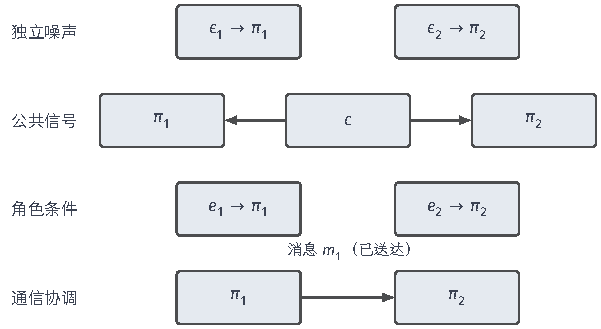
\includegraphics[width=101.741mm]{figures/10-reinforcement-learning/03-task-expansion-and-trustworthiness/tikz/rl-multi-agent-exploration.pdf}
 \caption{联合探索的四种动作与消息生成路径。独立噪声不能保证共同事件发生；公共信号、角色条件和通信分别提供协调依据，箭头表示执行者在动作前实际取得的观测、消息或随机信号。}
 \label{fig:rl-multi-agent-exploration}
\end{figure}

在公共信号例中，真实联合概率$\mathbb P(a_1=\text{按},a_2=\text{按})=0.1$，边缘概率的乘积却是0.01。若将后者作为行为概率，重要性权重就会错十倍。动作依赖通信或同一随机数时也须作同样检查：可以直接保存真实联合概率，也可以先保存使条件独立成立的信号，再计算条件概率的乘积。

% Outline: 7.3.3
\subsection{经验分布变化与目标覆盖检验}
\label{sec:rl-multi-agent-coverage}

取得联合交互记录后，先检查其生成策略、伙伴组成和采集协议是否仍适用于目标。由式\eqref{eq:rl-multi-agent-induced}，版本$k$的对手以$q^{(k)}$概率等待时，自身前进的诱导奖励为$-4+3q^{(k)}$。等待概率改变$\Delta q$，奖励就改变$3\Delta q$，后续状态占用也可能随通过概率变化。不过，版本号变化只是潜在漂移的线索；是否实际发生漂移，应结合分层统计、预测残差或已知策略概率判断。

随后要检查支持，即生成机制是否可能产生目标需要的事件。设日志只以各$1/2$概率生成$(0,0)$和$(1,1)$，非对角联合动作概率为0。每个人的两个动作都出现了，但$(0,1)$和$(1,0)$仍无支持。若两个奖励模型在对角线上都给0，在非对角线上却分别给$10$和$-10$，它们产生的日志分布完全相同，对候选偏离的预测却相反。这个反例表明：没有额外结构假设，边缘覆盖不足以识别未见的联合效果。

表\ref{tab:rl-multi-agent-support}按待估量列出需要检查的支持。实践中还须区分总体概率和样本频率：有限样本未出现某事件，不足以证明其总体概率为零，应连同频率报告不确定性。同样，未检出漂移也不足以证明生成机制恒定。

\begin{table}[htbp]
 \centering
 \begin{tabularx}{\linewidth}{@{}l >{\raggedright\arraybackslash}X >{\raggedright\arraybackslash}X@{}}
 \toprule
 估计对象 & 所需支持 & 典型缺失\\
 \midrule
 目标联合价值 & 目标到达状态及联合动作，目标伙伴 & 某种配合从未采到\\
 最佳响应 & 固定对手下候选完整策略的状态与动作 & 只记录原策略的到达状态\\
 个体反事实优势 & 固定其他动作后的自身候选动作 & 仅含对角动作的记录不能估非对角值\\
 消息条件价值 & 对应消息历史、角色、策略类型 & 未记消息使条件分布不可恢复\\
 \bottomrule
 \end{tabularx}
 \caption{待估量所需的联合支持及常见缺口。增加集中状态输入可以细化条件，却不能提供未发生的联合行为后果。}
 \label{tab:rl-multi-agent-support}
\end{table}

% Outline: 7.3.4
\subsection{覆盖充分时的可用经验构造}
\label{sec:rl-multi-agent-reweight}

目标事件有支持之后，还要处理来源比例与目标不一致的问题。只用最近窗口可缩小版本跨度，代价是丢弃旧版本策略产生的交互记录；按参与者分层可控制伙伴组成；将类型或版本输入价值网络，可分别估计不同对手条件下的后果。若已知生成概率，还可以用重要性校正把行为分布下的期望换为目标分布下的期望。这些措施分别改变样本选择、估计条件或期望测度，可以组合，但没有一种能无条件消除共同学习的非平稳性。

令$k$为一回合抽到的策略群体身份，$\tau$为长度$H$的完整理论轨迹，$q_\beta,q_\pi$分别为行为与目标的伙伴分布。要换算期望，先假设两过程具有相同的初始分布、联合反馈核$K$、环境终止规则和消息送达协议，并且目标联合轨迹分布对行为分布绝对连续，即目标有概率的事件在行为中也有概率。下面的$p_\pi,p_\beta$是相应完整轨迹律的质量函数或共同支配测度下的密度。将轨迹生成概率相除，得到
\begin{equation}
 w(\tau,k)=\frac{p_\pi(\tau,k)}{p_\beta(\tau,k)}
 =\frac{q_\pi(k)}{q_\beta(k)}
   \prod_{t=0}^{H-1}
   \frac{\bm\pi(\bm a_t\mid\bm I_t,k)}
        {\bm\beta(\bm a_t\mid\bm I_t,k)}.
 \label{eq:rl-multi-agent-is}
\end{equation}
两过程相同的联合反馈核项在比值中整体相消；这一步不要求后继状态、奖励、观测与终止反馈在核内独立。留下的是伙伴抽样与逐时刻联合动作的概率比。策略产生的消息若未包含在动作内，还须保留消息概率比；公共信号分布若改变，也须乘上其比值。只有给定记录历史与公共信号后各人条件独立，联合动作比才能分解为$\prod_i\pi_i(a_{i,t}\mid I_{i,t},k)/\beta_i(a_{i,t}\mid I_{i,t},k)$。据此，对完整轨迹函数$f$有$\mathbb E_\pi f=\mathbb E_\beta[wf]$；只估计某个时刻的奖励时，逐决策形式使用截至该奖励的前缀比，不必包含未来动作。

把该权重用于可见记录时，还须能从记录恢复计算概率比所需的动作历史、伙伴身份和消息字段。若$f$与$w$均可由记录计算，完整轨迹上的换测度等式也给出记录上的相应等式；丢弃这些必要字段后，应先边缘化得到记录密度比，不能直接沿用完整轨迹的乘积。

实际构造可以按来源分层取样，恢复真实条件概率，再以所得权重加权回报或损失。按上述个体条件分解计算时，长度$H$的轨迹需要计算$mH$个个体策略概率，还包括伙伴与信号概率。概率比连乘可能带来很大波动：每个个体比值为2时，十人同一步的乘积已经是1024，长轨迹还会继续累积。截断为$\min(w,c)$能限制极端样本影响，但所估期望也改为$\mathbb E_\beta[\min(w,c)f]$，由此产生的偏差必须报告。行为概率为零的事件则没有可加权的样本，不能通过设置无限大权重补回。

另一种处理历史策略回放记录的方法是策略指纹：把训练轮次、探索率等生成条件输入价值网络，使网络区分不同来源。它改变的是估计器读取的训练轮次、探索率等条件变量，不是概率测度，因此不带来重要性校正的无偏结论。多智能体经验回放中已有对两者的直接比较，结果仍限于相应任务和实现条件\scite{rl7-foerster2017replay}

% Outline: 7.3.5
\subsection{覆盖不足时的经验补充与学习边界}
\label{sec:rl-multi-agent-data-boundary}

若检查发现缺口，下一步由访问权限决定。有权继续采集时，可调整伙伴抽样以补充未见参与者，使用合法公共信号或通信探索未见联合动作；缺的是后续状态时，需要改变到达策略，仅在入口加噪声未必有用。若缺的是动作概率、消息等日志字段，应补充后续日志字段，已经丢失的历史通常无法追补。图\ref{fig:rl-multi-agent-data-loop}按访问权限标出哪些缺口可以回到采集环节。

\begin{figure}[htbp]
 \centering
 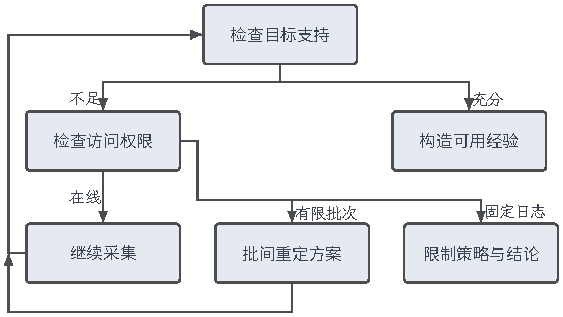
\includegraphics[width=95.282mm]{figures/10-reinforcement-learning/03-task-expansion-and-trustworthiness/tikz/rl-multi-agent-data-loop.pdf}
 \caption{覆盖缺口与记录访问权限决定的处理路径。在线访问允许补采，有限批次只允许批间调整；固定日志不能继续交互，须限制目标或明确引入可检验假设。}
 \label{fig:rl-multi-agent-data-loop}
\end{figure}

有限批次可采用如下协议：总共$B$批，第$b$批包含$N_b$个联合环境步；批内冻结行为策略、伙伴抽样与探索规则，批结束后再按反馈选择第$b+1$批方案。若对手在内部在线适应，须将其适应规则作为策略的一部分声明，并记录所依赖的历史，不能将它称为固定的状态条件对手。只有固定日志时，可将策略限制在有支持的区域、增加可检验结构假设，或按第\ref{chap:rl-information}章采用悲观评价。网络容量再大，也不能从相同日志中区分前述两个奖励模型，因而不能单独解决不可识别性。

% Outline: 7.4
\section{不同参与者依赖下的行为后果估计}
\label{sec:rl-multi-agent-estimation}

联合经验有了明确来源、也确认了覆盖后，估计“某个动作的后果”仍有多种做法，区别在于保留多少参与者之间的依赖。可以把所有人的当前动作都保留下来，估计一个完整的联合价值；也可以固定其他人的动作，只比较我换成别的动作会怎样（个体反事实）；还可以假定联合价值能由各人的局部效用组合而成（局部分解）；或者干脆去预测伙伴会怎么行动，把伙伴的行为显式建进模型；更复杂时，还要计入“我的改变会诱发伙伴如何回应”。这五种估计方式回答不同问题、服务不同计算，可以叠加使用。例如集中训练的评论家可以同时以伙伴类型为条件、又输出固定他人动作后我的全部候选动作价值；群体学习器也可以用单调分解来计算近似的相互响应。

% Outline: 7.4.1
\subsection{基于联合行为的后果估计}
\label{sec:rl-multi-agent-joint-value}

先考虑利用全局状态、联合动作及所需历史的集中评价：固定要评价的联合策略$\bm\pi$，把当前所有人的动作也作为输入，估计一个完整的联合动作价值。做这种集中评价时，评论家用于递推的条件变量$x_t$必须足以预测它会产生的后继过程：完全可观测且策略无记忆时可取$s_t$，策略依赖历史时则要取$(s_t,\bm I_t)$。
\begin{align}
 Q_i^{\bm\pi}(x,\bm a)
 &=\mathbb E[G_{i,t}\mid x_t=x,\bm a_t=\bm a],\\
 V_i^{\bm\pi}(x)
 &=\sum_{\bm a}\bm\pi(\bm a\mid x)Q_i^{\bm\pi}(x,\bm a).
\end{align}
其中$Q_i$评价本次联合动作已确定、随后照$\bm\pi$执行的长期后果，$V_i$还按现有策略平均本次动作。$\bm\pi(\bm a\mid x)$只是在集中条件变量$x$下写出各合法局部策略产生的分布，并未授予行动者读取整个$x$的权限。若现有策略不给某个合法联合动作正概率，其$Q_i$仍可通过从$x$强制执行该动作、随后遵循$\bm\pi$的过程定义；不能用零概率事件上的条件期望唯一确定它。

为从训练样本中的联合转移记录递推这些价值，将回报拆成即时奖励与折扣后的后继回报，再对后继集中条件变量及联合动作取条件平均，得到Bellman评价式
\begin{equation}
 Q_i^{\bm\pi}(x,\bm a)=R_i(x,\bm a)+
 \gamma\sum_{x',d}T_x(x',d\mid x,\bm a)(1-d)
       \sum_{\bm a'}\bm\pi(\bm a'\mid x')Q_i^{\bm\pi}(x',\bm a').
 \label{eq:rl-multi-agent-joint-bellman}
\end{equation}
连续空间中，相应求和改为积分。上式只使用期望的线性分解，没有假设$r_i$、$x'$与$d$条件独立。训练时可用一条完整联合反馈样本替代条件期望，构造
$y_i=r_i+\gamma(1-d)V_{i,\text{目标}}(x')$，再最小化$(Q_{i,\bm\phi}(x,\bm a)-y_i)^2$作TD更新。这里$d$只表示真实终止：终止后没有后继回报，因而乘$1-d$；采样截断但过程未终止时，仍须保留后继价值。日志必须按第\ref{sec:rl-multi-agent-records}节保存或重建与当前接口一致的$x'$。

若要按零和或Nash标准选择后续行为，Minimax-Q将内层策略平均换成零和阶段价值，Nash-Q换成选定均衡的收益。此时进行的是控制备份，而不是对同一个固定$\bm\pi$的评价。即使保留集中训练，也未必需要输入当前联合动作。多智能体深度确定性策略梯度（multi-agent deep deterministic policy gradient, MADDPG）使用动作价值，评价各人的连续动作组合；多智能体PPO（multi-agent PPO, MAPPO）使用状态价值，作为采样回报的比较基准。表\ref{tab:rl-multi-agent-critics}比较这两种评论家接口。

\begin{table}[htbp]
 \centering
 \begin{tabularx}{\linewidth}{@{}l >{\raggedright\arraybackslash}X >{\raggedright\arraybackslash}X@{}}
 \toprule
 方法 & 训练输入与评价对象 & 策略更新与执行\\
 \midrule
 MADDPG & 集中条件变量$x$及$\bm a$；各自$Q_i(x,\bm a)$ & 对自身动作求价值梯度；执行仅用局部输入的确定性行动者\\
 MAPPO & 集中状态或联合观测，可补个体观测或角色标签；$V_i(x)$或团队$V(x)$ & 用回报与$V$构造优势；执行仅用局部输入的随机行动者\\
 \bottomrule
 \end{tabularx}
 \caption{集中动作价值与状态价值的两种接口。联合观测是否足以预测后继过程仍须论证；状态价值评论家不必输入当前联合动作。}
 \label{tab:rl-multi-agent-critics}
\end{table}

MADDPG用集中动作价值指导确定性行动者，可处理合作或竞争收益。MAPPO研究则在合作任务中考察集中状态价值怎样配合PPO，报告的是相应实现条件下的经验表现。两者使用不同评论家，并不意味着集中训练天然优于其他训练权限\scite{rl7-lowe2017,rl7-yu2022}

两种接口都依赖联合轨迹，需承担集中状态与联合历史的传输、价值网络前后向计算和联合轨迹存储成本。这些集中条件变量可帮助区分他人动作的作用，却既不冻结他人策略，也不消除函数逼近误差。尤其当$x$只含当前观测、遗漏对方记忆时，式\eqref{eq:rl-multi-agent-joint-bellman}所需的Markov条件仍可能缺失。训练得到价值之后，行动者还须遵守第\ref{sec:rl-multi-agent-permissions}节的执行权限。

% Outline: 7.4.2
\subsection{基于个体行为反事实的后果估计}
\label{sec:rl-multi-agent-counterfactual}

合作任务里只有一个共同奖励，于是会出现“功劳算谁的”问题：一次成功通过，究竟是因为我主动前进，还是因为对方及时等待？这就是团队中的信用分配。它最干净的形式可以先在一步任务里看清：把入口截成“一次联合动作后立即终止”的独立矩阵任务（故动作价值等于即时奖励），下一小节的表示反例也沿用这一约定。

要量化个人贡献，一种直接的做法是：先规定一个参照动作$c_i$（代表“我本来可以怎么做”），再比较“我实际这么做”和“换成参照、其他人不动”两种情况下的团队奖励之差，称为\term{差分奖励}（difference reward）：
$D_i=R(x,\bm a)-R(x,(c_i,\bm a_{-i}))$。已知上述一步奖励表时，取$c_1=W$得到$D_1=3$。实际交互只执行了一个联合动作，通常没有替代动作的第二份实测结果，而且替代动作还可能改变后继状态。因此，差分的来源须明确为模型、额外试验或价值估计，不能把它作为原日志中已经观察到的事实。

若要指导长期策略更新，需比较候选动作的回报价值，而不只比较即时奖励。反事实多智能体策略梯度（counterfactual multi-agent policy gradients, COMA）用当前策略规定参照：保持其他人的本次动作$\bm a_{-i}$不变，将$i$的候选动作价值按$\pi_i$平均作基线，再与实际动作价值相减：
\begin{align}
 b_i(x,\bm a_{-i})
 &=\sum_{\tilde a_i}\pi_i(\tilde a_i\mid I_i)
       Q^{\bm\pi}(x,(\tilde a_i,\bm a_{-i})),\\
 A_i^{\text{COMA}}(x,\bm a)
 &=Q^{\bm\pi}(x,\bm a)-b_i(x,\bm a_{-i}).
 \label{eq:rl-multi-agent-coma}
\end{align}
例如，1以$1/4$概率前进、$3/4$概率等待且2已等待时，上述一步任务的基线为
$\tfrac14(2)+\tfrac34(-1)=-1/4$，前进的优势为$9/4$。它小于固定以等待为参照的差分3，是因为基线比较当前策略的平均动作，而非固定动作$W$。

依赖别人实际动作的基线，是否会改变策略梯度的期望？先将获准使用的公共信号纳入各$I_i$，并要求给定足以描述联合后继过程的条件变量$x$和其他动作$\bm a_{-i}$后，$i$的条件动作分布仍为$\pi_i(\cdot\mid I_i)$。在策略可微、支持固定且得分与基线的乘积可积时，$b_i(x,\bm a_{-i})$不随本次抽到的$a_i$改变；更新中还须把它视为常数，停止通过基线反向传播。因而可以将它提出动作求和：
\begin{align}
 &\mathbb E_{a_i\mid x,\bm a_{-i}}
   [\nabla_{\bm\theta_i}\log\pi_i(a_i\mid I_i)b_i(x,\bm a_{-i})]\nonumber\\
 &\quad=b_i(x,\bm a_{-i})
       \sum_{a_i}\nabla_{\bm\theta_i}\pi_i(a_i\mid I_i)=0.
 \label{eq:rl-multi-agent-baseline-zero}
\end{align}
最后一步使用概率归一化：$\sum_{a_i}\pi_i(a_i\mid I_i)=1$，对参数求导为零。再平均$(x,\bm a_{-i})$就得到基线项零均值，承接定理\ref{thm:rl-learning-baseline}。若两人共享未记录的随机信号，给定$\bm a_{-i}$后的自身分布可能不再是$\pi_i$，推导中的替换就失效。需要在真实联合策略中处理相关信号，重新推导得分与基线；只将得分改成另一个条件分布的对数梯度，还不足以证明估计的仍是原目标梯度。

为计算该基线，COMA评论家可一次输出自身全部候选动作价值，避免逐个候选运行完整网络。但输出规模仍随$|\mathsf A_i|$增长，连续动作还需近似积分。评论家的训练目标来自联合轨迹，未执行候选的价值仍是估计，而非新增观测。原方法据此将集中评论家与分散行动者连接起来\scite{rl7-foerster2018coma}

零均值结论只保证从精确价值中减去该基线不改变策略梯度期望，并不保证任何基线都降低方差；评论家误差还可能使优势估计失真。此处的“反事实”指固定他人当前动作的候选价值比较，不能据此宣称识别了因果结构模型中唯一真实的个人贡献。

% Outline: 7.4.3
\subsection{基于局部行为组合的后果估计}
\label{sec:rl-multi-agent-factorization}

联合价值回答了“整组动作有多好”，但部署时每个人只能在本地独立选择自己的动作，他既看不到联合价值表、也无法和所有人实时联合优化。于是需要另一种结构：让每个人只计算一个依赖本地历史的局部效用，再保证“每个人都选本地最优”这件事拼起来恰好等于“联合动作最优”。形式地说，设各人只能计算局部效用$q_i(I_i,a_i)$并各自执行$a_i^*\in\arg\max_{a_i}q_i(I_i,a_i)$，所有局部贪心动作能组成联合贪心动作这一性质称为\term{个体与整体最大化一致性}（individual-global-max, IGM）；这里效用是帮助组合团队行为的内部量，不必等于$i$自己的环境回报。

\Needspace{24\baselineskip}
图\ref{fig:rl-multi-agent-mixers}给出两种实现这种一致性的结构。价值分解网络（value decomposition networks, VDN）直接设$Q_{\text{tot}}=\sum_i q_i$，把各人的局部效用相加；单调价值函数分解方法QMIX（monotonic value function factorisation）允许训练状态决定混合器参数，但以非负权重和单调激活保证$\partial Q_{\text{tot}}/\partial q_i\geq0$。提高任一局部效用不会降低联合值，因此部署时可只保留局部贪心选择，无须读取状态。实现这一便利的代价，是分别将联合价值限制为加和或单调组合\scite{rl7-sunehag2018,rl7-rashid2018}

以下充分条件将“不降低联合值”的性质转成对局部贪心动作的保证。

\begin{theorem}[单调组合的局部贪心充分性]
\label{thm:rl-multi-agent-monotone}
固定评论家条件变量$x$及所有局部历史，假设联合动作集合是各人动作集合的笛卡尔积，且局部最大值都存在。若
\[
 Q_{\text{tot}}(x,\bm a)
 =f_x(q_1(I_1,a_1),\ldots,q_m(I_m,a_m))
\]
对每个局部效用逐坐标非减，就有
\[
 \prod_i\arg\max_{a_i}q_i(I_i,a_i)
 \ \subseteq\ \arg\max_{\bm a}Q_{\text{tot}}(x,\bm a).
\]
\end{theorem}
\begin{proof}
任取一组局部最大化动作$\bm a^*$，从任意联合动作$\bm a$开始逐个替换分量。第一分量改为$a_1^*$时，$q_1$不下降，其余效用保持不变；由$f_x$对第一坐标非减，联合值也不下降。第二分量改为$a_2^*$时理由相同，依次完成$m$次替换便有
$Q_{\text{tot}}(x,\bm a)\leq Q_{\text{tot}}(x,\bm a^*)$。由于起点$\bm a$任意，$\bm a^*$最大化联合值；又因为任意局部最大化组合都可作上述替换，故得到所述包含关系。
\end{proof}

保证方向仅从局部最大化指向联合最大化，不能无条件写成等号。例如$f_x$为常数时，全部联合动作都最优，$q_1$却可以只有一个最大化动作；平台区间与并列效用也会造成差别。若合法动作之间存在耦合约束，各人合法动作的乘积可能包含非法组合，逐分量替换就未必保持可行，需重新检验证明条件。

\begin{figure*}[htbp]
 \centering
 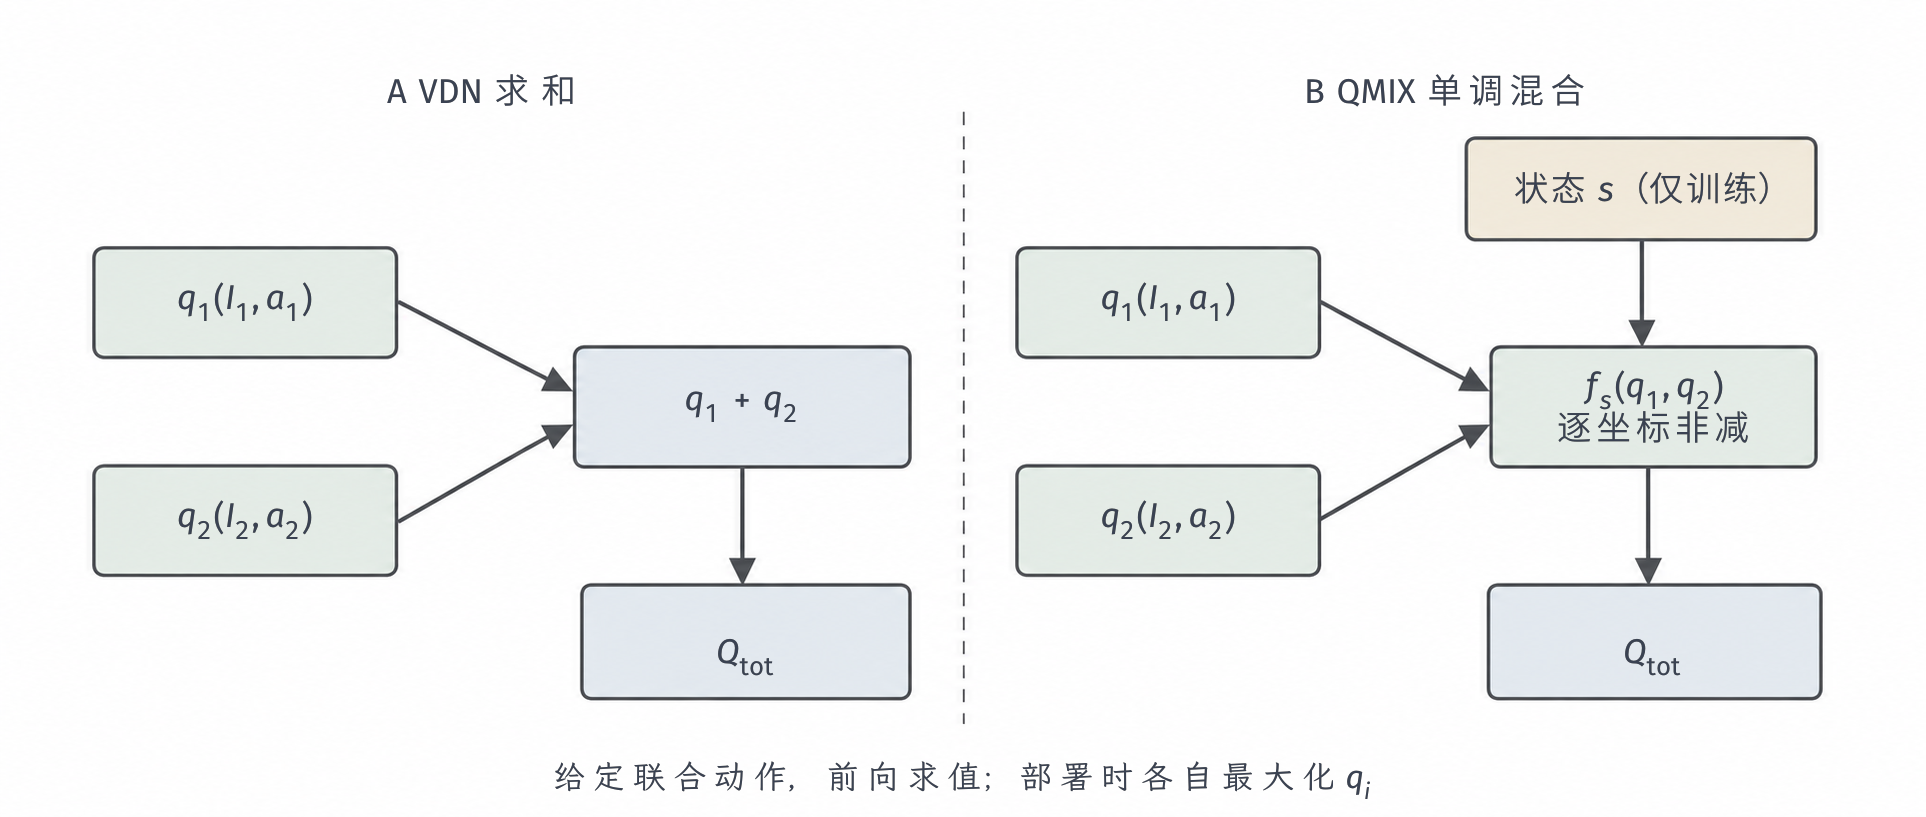
\includegraphics[width=157.400mm]{figures/10-reinforcement-learning/03-task-expansion-and-trustworthiness/generated/rl-multi-agent-mixers/figure.png}
 \caption{给定联合动作时，VDN与QMIX由标量局部效用$q_i(I_i,a_i)$组合联合价值。图中只画前向求值；训练时联合TD损失经求和或单调混合器向全部局部效用网络反传。状态仅供QMIX训练混合器使用，部署时各人选择自身$q_i$的最大化动作。}
 \label{fig:rl-multi-agent-mixers}
\end{figure*}

单调表示的限制也可以在入口一步奖励表中检验。对方前进时，1等待更好；对方等待时，1前进更好，即两列分别要求
$Q(F,F)<Q(W,F)$和$Q(F,W)>Q(W,W)$。若局部排序$q_1(F)>q_1(W)$，第一列违反非减性；若排序相反，第二列违反；若二者相等，单调混合器在两列都不能产生严格差别。因而固定历史下的标量局部效用不能用这一结构精确表示整张表。然而“1前进、2等待”的固定约定仍可分散执行并取得最优奖励。整表可表示、最优动作可执行与训练能找到该动作，是需要分别验证的三件事。

\Needspace{16\baselineskip}
若任务需要更丰富的价值模式，可以放松或改写组合约束，表\ref{tab:rl-multi-agent-factorization}列出两种方式。QTRAN用价值变换和一致性约束保持最优动作；QPLEX以优势分解表示更一般的IGM结构。它们扩大的是表示能力，不是行动者可读取的观测、历史和消息范围。结构在理论上能表示某种值，还须与实际训练是否满足约束、函数逼近误差及优化误差分开判断\scite{rl7-son2019,rl7-wang2021qplex}

\begin{table}[htbp]
 \centering
 \begin{tabularx}{\linewidth}{@{}l >{\raggedright\arraybackslash}X >{\raggedright\arraybackslash}X@{}}
 \toprule
 结构 & 保留的限制或分解 & 代价与边界\\
 \midrule
 VDN & 联合价值为局部效用之和 & 组合便宜；不能表达一般相互作用\\
 QMIX & 状态条件的逐坐标非减混合 & 增加混合器；局部排序不能随他人动作反转\\
 QTRAN & 联合价值与易分解变换在贪心处相等、其他动作满足不等式 & 需拟合联合值并施加约束；近似惩罚不保证精确满足\\
 QPLEX & 局部优势$q_i-\max q_i\leq0$以正权组合，另建联合基准值 & 优势与权重结构增加表达力；表示充分性不等于优化收敛\\
 \bottomrule
 \end{tabularx}
 \caption{局部价值组合的表示限制与代价。更换组合结构不妨碍同时使用伙伴条件化、回放管理或群体训练。}
 \label{tab:rl-multi-agent-factorization}
\end{table}

这些结构都可从联合转移构造团队TD目标，并把损失反传到局部网络。差别在于怎样计算目标中的最大值，以及可以容纳哪些联合价值模式。每人有$A$个动作时，直接枚举需处理$A^m$个组合；局部贪心只比较$mA$个效用，再调用混合器。降低的是动作最大化的计算成本，不能据此断言同样数量的样本足以准确学习所有效用。

% Outline: 7.4.4
\subsection{基于其他参与者策略的行为后果估计}
\label{sec:rl-multi-agent-opponent-model}

前面都假定别人的行为已知，但现实中伙伴的策略通常是隐藏的，只能通过交互去推断。关键的直觉是：即使我当前动作完全相同，不同类型的伙伴也会让后果不同。

要把对伙伴类型的判断写成可更新的概率分布，令伙伴信念$b_t(z)=\mathbb P(z\mid I_{i,t})$，即仅依据获准历史形成的类型分布。自身动作$a_{i,t}$可能改变随后看到的证据$e_{t+1}$，故用$\ell(e_{t+1}\mid I_{i,t},a_{i,t},z)$表示相应似然。若动作只依据已记录历史和独立随机数产生，其选择概率不随候选类型变化，可在贝叶斯归一化时相消。于是用新证据更新信念：
\[
 b_{t+1}(z)=
 \frac{\ell(e_{t+1}\mid I_{i,t},a_{i,t},z)b_t(z)}
      {\sum_{\tilde z}\ell(e_{t+1}\mid I_{i,t},a_{i,t},\tilde z)b_t(\tilde z)}.
\]
此更新要求分母大于0，即至少一个具有正先验概率的类型对所见证据赋予正似然。若动作选择使用了未记录的类型线索，动作概率就不能直接消去。若没有直接观察伙伴动作，似然还须对隐藏动作、状态或消息求和，不能在部署辨识中读取仅供训练的真实动作标签。类型若外生变化，则先通过类型转移核预测，再由证据校正。这里与式\eqref{eq:rl-transfer-belief-update}的贝叶斯步骤相同，变化的是推断对象：从任务条件转为参与者行为。

信念可用于评价候选动作。令$Q_i(I_i,b,a_i,z)$表示固定类型$z$下执行$a_i$，随后按同一套策略及信念更新规则行动的条件回报，则全期望公式给出
$Q_i(I_i,b,a_i)=\sum_z b(z)Q_i(I_i,b,a_i,z)$。
各项都须平均尚未观察的伙伴动作和状态，不能为每个类型偷偷换用“已知类型时”的最优策略，否则平均后不再对应实际可执行行为。后续若继续辨识类型，价值状态与递推也须保留信念更新；把信念冻结的近似会遗漏探测反馈对后续动作选择及回报的影响。

类型模型也可不用有限标签，而用历史编码器输出一个向量，再由该向量预测下一动作的分布。训练时最小化可见动作的负对数似然，即提高模型赋给实际观察动作的概率，学得的表示再输入条件评论家或策略。每次更新需支付历史编码、似然预测及候选动作评价的计算成本，不必直接读取对方网络参数。身份、检查点版本和潜在类型仍不能混为一谈，同一身份可以改用策略，不同身份也可能行为相同。上述估计将对手视为固定或外生变化，尚未计入自身更新诱发的响应。

% Outline: 7.4.5
\subsection{基于参与者相互响应的行为后果估计}
\label{sec:rl-multi-agent-response-model}

比“伙伴类型固定”更进一步的是：伙伴也在学习、会对你的改变作出反应。自身行为改变后，对方可能让步，也可能采用更强硬的规则；只拟合他当前的等待率，就漏掉了“我的策略改变会诱发他如何回应”这一条影响途径。

在两人问题中，固定响应前的对方参数$\bm\psi_0$，以
$\bm\psi'=\mathcal R(\bm\theta_i;\bm\psi_0)$表示对方看到$i$的策略或交互之后采用的参数，$J_{-i}$为对方目标。若$\mathcal R(\bm\theta_i;\bm\psi_0)=\bm\psi_0$，就回到固定对方的估计。若预测对方作一步学习，可规定
$\bm\psi'=\mathcal R(\bm\theta_i;\bm\psi_0)
=\bm\psi_0+\eta\left.\nabla_{\bm\psi}J_{-i}(\bm\theta_i,\bm\psi)\right|_{\bm\psi=\bm\psi_0}$，其中求响应映射对$\bm\theta_i$的导数时保持$\bm\psi_0$固定。这一规则还要求说明它使用的目标、当前策略和用于估计梯度的联合轨迹训练样本。继续增加推理层次时，还须规定对方是否知道$i$的更新规则、是否也预测$i$；增加递归深度会增加假设，而非自动增加准确性。

为区分自身直接改变与对方响应的影响，若$J_i$及$\mathcal R$在所考察邻域可微，可对复合回报使用链式法则：
\begin{equation}
 \nabla_{\bm\theta_i}J_i(\bm\theta_i,\mathcal R(\bm\theta_i;\bm\psi_0))
 =
 \left.\partial_{\bm\theta_i}J_i(\bm\theta_i,\bm\psi)
       \right|_{\bm\psi=\bm\psi'}
 +[D_{\bm\theta_i}\mathcal R(\bm\theta_i;\bm\psi_0)]^\top
 \left.\nabla_{\bm\psi}J_i(\bm\theta_i,\bm\psi)
       \right|_{\bm\psi=\bm\psi'}.
 \label{eq:rl-multi-agent-response-gradient}
\end{equation}
右侧两个回报偏导都在响应后的$(\bm\theta_i,\bm\psi')$处评价：第一项求导时固定$\bm\psi'$，第二项再用响应映射的Jacobian把对方参数变化传回自身参数；$D_{\bm\theta_i}\mathcal R$则在响应前参数$\bm\psi_0$固定时求得。

用一个独立的单步通道变体演示这两条途径。自己以前进概率$p$行动，对方以前进概率$q$行动，给定$p,q$后两人独立随机化；自己前进且对方等待时得1，其余结果得0，一步后终止。因此自身期望回报为$J(p,q)=p(1-q)$。假设对方观察到自己的策略后采用$q(p)=0.8-0.6p$，$p\in[0,1]$；此时$q$始终在$[0.2,0.8]$内。这个响应函数是教学假设，计分也与前面$-1/-4$的通道任务分开。

在内部点$p_0\in(0,1)$，先固定已经响应的$q(p_0)$，直接改变$p$所得导数为$1-q(p_0)=0.2+0.6p_0$。再计入对方前进概率的变化，间接项为$-p_0q'(p_0)=0.6p_0$，两者合计$0.2+1.2p_0$。也可先代入得到$J(p,q(p))=0.2p+0.6p^2$再求导，得到相同结果。若始终把对方固定为$q=0.8$，目标就是$0.2p$，导数才恒为0.2；两种计算对应不同的响应假设。

一步学习响应还需对对方的梯度更新求导，因而涉及梯度的导数；只有交互观测时则要先拟合响应模型，承担相应误差。学习感知的对方学习（learning with opponent-learning awareness, LOLA）据对方学习步骤构造了此类更新\scite{rl7-foerster2018lola}

式\eqref{eq:rl-multi-agent-response-gradient}暂将$\mathcal R$视为确定映射。若它由随机采集的训练样本更新产生，对一份固定样本求导仅得到条件导数；若训练样本的采集律也随$\bm\theta_i$变化，完整期望梯度还包含分布的导数。第\ref{sec:rl-transfer-value-training}节的元学习目标同样区分了固定样本求导与对采样过程求导。

若最佳响应多解或不连续，式\eqref{eq:rl-multi-agent-response-gradient}的可微映射假设可能不成立；对手若不按所设规则学习，求得的导数也只描述错设模型。更深层推理会提高计算成本并放大这种风险。预测下一次响应只是预测任务；斯塔克尔伯格式（Stackelberg）承诺解要求先行者公开承诺策略，后行者据此作最佳响应，因而还须有可承诺、可观察的先后行动协议。同时行动下的Nash均衡又要求固定他人策略后检验单方偏离。三者不能凭响应模型的复杂程度相互替代。

% Outline: 7.5
\section{多智能体的策略更新与学习动态}
\label{sec:rl-multi-agent-learning}

有了价值与优势，还要规定策略如何据此更新，而多智能体的更新比单人多了两个层面的牵连。一个训练批次可以产生价值更新或梯度步；与此同时，各学习者既可以只针对当前对手响应，也可以针对历史上出现过的行为响应；训练对手还可以由一个不断扩充的策略群体来安排配对。例如“从策略库中抽对手，再用策略梯度训练近似最佳响应，最后把新响应加回库”，就同时规定了三件事：更新怎么算（梯度/价值）、相互如何适应（对库中对手）、以及训练群体如何组织（扩充策略库）。下面分别讲清这三个环节，最后再追问：当大家都在同时学习时，这个过程是否稳定、能保证什么。

% Outline: 7.5.1
\subsection{由价值与梯度计算策略更新}
\label{sec:rl-multi-agent-update}

先在本轮计算中冻结其他策略与目标评论家。对训练批次$D_{\mathrm{batch}}$中的联合转移求后继目标，再拟合价值或构造优势，最后得到新动作规则或新策略参数。表\ref{tab:rl-multi-agent-value-updates}按这条路径比较几种价值方法。独立Q学习把他人行为边缘化，只有条件变量足以预测诱导后继过程、诱导环境平稳等前提成立，才能援引表格型单智能体Q学习保证；共同更新、压缩局部历史或使用函数逼近，都可能破坏这些前提。

\begin{table}[htbp]
 \centering
 \begin{tabularx}{\linewidth}{@{}l >{\raggedright\arraybackslash}X >{\raggedright\arraybackslash}X >{\raggedright\arraybackslash}X@{}}
 \toprule
 方法 & 价值输入 & 后继备份 & 动作与执行时可读变量\\
 \midrule
 独立Q & $I_i,a_i$ & 自身$\max Q_i$ & 局部贪心；他人行为被边缘化\\
 Minimax-Q & $s,\bm a$ & 零和矩阵价值 & 按解出的混合策略抽样；需状态\\
 Nash-Q & $s,\bm a$的各人收益 & 选定阶段均衡收益 & 按同一均衡选择约定；需状态\\
 VDN & 局部$I_i,a_i$再求和 & 局部最大值之和 & 每人局部贪心\\
 QMIX & 局部效用与训练状态 & 单调混合的局部最大值 & 每人局部贪心；执行无须状态\\
 \bottomrule
 \end{tabularx}
 \caption{由价值目标生成动作的不同接口。各行仍需规定联合采样、终止处理和目标网络；即使算出了阶段博弈解，也须检查执行所需的状态、观测或公共建议是否可读。}
 \label{tab:rl-multi-agent-value-updates}
\end{table}

一条教学样本即可显示参数化怎样影响更新。设通道样本奖励$r=2$，尚未终止，目标网络给后继联合值1，$\gamma=0.9$，则目标$y=2.9$。当前$Q=1$时，对$\tfrac12(Q-y)^2$作步长0.1的表格梯度下降，残差$-1.9$使新值为$Q'=1.19$。若改用VDN且两个局部效用为0.4和0.6，同一残差分别传到两个表项，一次同步更新后为0.59和0.79，联合值为1.38。联合值的变化不同，是因为两个参数同时改变了有效步长。QMIX传回残差时还须乘混合器对各效用的导数；Minimax-Q与Nash-Q则须为后继目标运行阶段求解器。

随机行动者也可直接沿收益梯度更新。令$\bm\pi_{\bm\theta}=\prod_i\pi_{\bm\theta_i}(a_i\mid I_i)$，暂不共享参数，并固定其他参数与环境机制。假设策略可微、支持固定，同时满足式\eqref{eq:rl-learning-policy-gradient}所需的可积支配条件，以便交换求导与折扣求和。对轨迹概率取对数后，只有$i$的动作项依赖$\bm\theta_i$；每次动作的得分只需乘其后回报，先前奖励对应的得分期望为零。将未来奖励归并为$G_{i,t}$，再用折扣占用表示时刻求和，得到
\begin{align}
 \nabla_{\bm\theta_i}J_i(\bm\pi)
 &=\sum_{t\geq0}\gamma^t
   \mathbb E_{\bm\pi}
   [\nabla_{\bm\theta_i}\log\pi_i(a_{i,t}\mid I_{i,t})G_{i,t}]
 \nonumber\\
 &=\frac{1}{1-\gamma}
   \mathbb E_{x,\bm a\sim d^{\bm\pi}}
   [\nabla_{\bm\theta_i}\log\pi_i(a_i\mid I_i)
           Q_i^{\bm\pi}(x,\bm a)].
 \label{eq:rl-multi-agent-policy-gradient}
\end{align}
这里$d^{\bm\pi}$是集中条件变量$x$与联合动作上的归一化折扣占用度量，它包含归一化因子$1-\gamma$；目标$J_i$未归一化，故第二行须保留$1/(1-\gamma)$。减去符合条件的基线可将$Q_i$换成优势。若联合策略相关，则要从真实联合概率重新推导得分，并检查第\ref{sec:rl-multi-agent-counterfactual}节的基线条件，不能直接使用各人边缘策略的得分。

此梯度把行动者局部历史与评论家集中条件变量的两种用途分开：行动者以自身局部历史计算动作得分，集中评论家提供该动作的长期后果估计。在一步终止的入口教学样本中，若前进概率$p=1/4$由logit参数生成，即以$p/(1-p)$的对数表示参数，采到$(F,W)$并采用前节精确优势$9/4$，得分为$1-p=3/4$，乘积为$27/16$。步长0.1使logit由$\log(1/3)$增至$\log(1/3)+27/160$，前进概率约为0.283。这里直接更新有限一步样本，没有使用归一化折扣占用，因此不额外乘其系数。

\Needspace{7\baselineskip}
PPO类更新用旧策略产生批次，计算自身动作的概率比$\zeta_{i,t}=\pi_i(a_{i,t}\mid I_{i,t})/
\pi_i^{\text{旧}}(a_{i,t}\mid I_{i,t})$，再最大化以下裁剪代理目标的批次均值：
\[
 \min\{\zeta_{i,t}\widehat A_{i,t},
       \operatorname{clip}(\zeta_{i,t},1-\epsilon,1+\epsilon)
                      \widehat A_{i,t}\}.
\]
其中$\widehat A_{i,t}$为优势估计，$0<\epsilon<1$规定围绕概率比1的裁剪宽度；取两项较小值，限制概率比在有利方向上继续扩大代理目标。独立PPO以局部价值估计优势，MAPPO则用集中状态价值。这里的自身概率比没有包含其他动作和后续轨迹，不能等同于完整联合轨迹的重要性比。同批次反复更新所有人时，对手与状态分布均可能变化，所以裁剪机制本身不构成共同学习的单调改进证明。

对连续可微动作，确定性行动者$a_i=f_{\bm\theta_i}(I_i)$可直接对动作价值使用链式法则。精确同策略梯度中的局部方向为
$\nabla_{\bm\theta_i}f_{\bm\theta_i}(I_i)\nabla_{a_i}Q_i^{\bm f}(x,\bm a)$，以归一化$d^{\bm f}$表示时同样带$1/(1-\gamma)$。MADDPG用目标行动者生成后继动作，由联合回放的TD损失拟合$Q_i$，再估计这一方向；用回放分布替代$d^{\bm f}$得到的是离策略代理更新，未经校正不能称为原$J_i$的无偏梯度。COMA保留随机行动者，采用式\eqref{eq:rl-multi-agent-coma}的优势。表\ref{tab:rl-multi-agent-policy-updates}按计算与采样条件比较这些接口。

\begin{table}[htbp]
 \centering
 \begin{tabularx}{\linewidth}{@{}l >{\raggedright\arraybackslash}X >{\raggedright\arraybackslash}X@{}}
 \toprule
 方法 & 价值、采样与策略方向 & 主要成本或失效处\\
 \midrule
 独立PPO & 近期联合轨迹中的局部$V_i$与裁剪得分梯度 & 价值未以其他人的动作或历史为条件；同时更新漂移\\
 MADDPG & 联合回放$Q_i$与确定性动作梯度 & 集中动作输入、回放失配、评论家动作梯度误差\\
 MAPPO & 近期轨迹中的集中$V_i$与裁剪得分梯度 & 集中状态传输、优势误差、批内复用漂移\\
 COMA & 联合$Q$与固定其他动作的候选基线 & 枚举自身候选；未见动作价值估错\\
 \bottomrule
 \end{tabularx}
 \caption{策略梯度接口的价值、采样和成本差异。梯度所针对的$J_i$由收益设定决定，不能由方法名称推断合作或竞争目标。}
 \label{tab:rl-multi-agent-policy-updates}
\end{table}

这些更新只沿图\ref{fig:rl-multi-agent-ctde}的训练梯度路径传递，部署动作仍由各人的局部决策历史及获准消息生成。团队若共享参数$\bm\theta$，每个人的动作概率都依赖它，轨迹得分便为$\sum_i\nabla_{\bm\theta}\log\pi_{\bm\theta}(a_i\mid I_i)$，用于汇总共同$J$的梯度。若各人$J_i$不同而参数仍共享，就须另定加权目标或更新调度。直接平均冲突梯度也已选择了收益取舍，不能视为不改变目标的实现细节。

% Outline: 7.5.2
\subsection{多个学习者之间的相互适应}
\label{sec:rl-multi-agent-mutual-learning}

即使每个学习者各自的更新方向都确定无误，多人一起更新时的“时序安排”仍会显著改变学习轨迹，因为每个人面对的对手都是一个移动目标。这里有一个带点反直觉、但在零和学习中很关键的现象：两个人各自针对“旧的对方”做改进，并不保证他们合起来在向均衡靠近——双方同时迈一步，可能只是在均衡点周围旋转甚至越转越远。下面用最简单的匹配硬币博弈把这种差别算清楚。记$p,q$分别为第一人、第二人选择其第一个动作的概率。
\[
 p^{(k+1)}=[p^{(k)}+\eta(4q^{(k)}-2)]_{[0,1]},\qquad
 q^{(k+1)}=[q^{(k)}-\eta(4p^{(k)}-2)]_{[0,1]}.
\]
若改为交替更新，先计算$p^{(k+1)}$，第二式就使用这一新值而非$p^{(k)}$。图\ref{fig:rl-multi-agent-trajectories}以同一$\eta=0.1$和初值$(0.7,0.5)$迭代两种规则；第三条历史响应曲线则对截至上轮的平均对手求精确最佳响应，平局时选$1/2$。这样可以在同一博弈中区分更新时序和响应对象的影响。

\begin{figure*}[htbp]
 \centering
 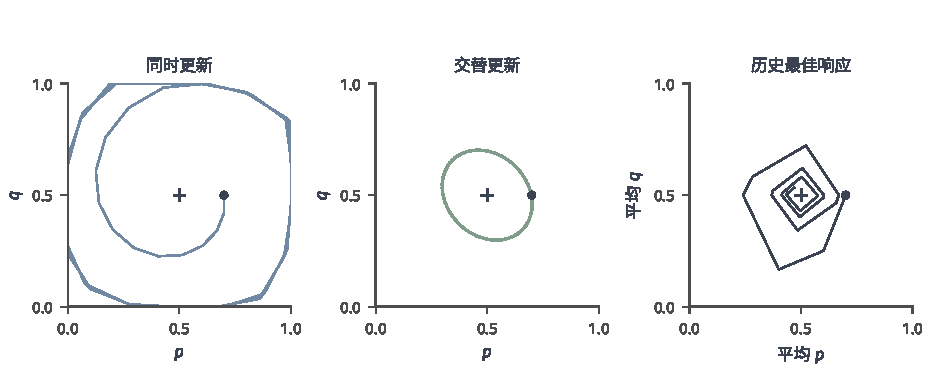
\includegraphics[width=157.400mm]{figures/10-reinforcement-learning/03-task-expansion-and-trustworthiness/matplotlib/rl-multi-agent-trajectories.pdf}
 \caption{匹配硬币博弈中三种响应规则的120次更新。曲线由图源递推式计算，并非实验成绩；圆点标初值，十字标均衡$(1/2,1/2)$，历史响应面板显示累计平均策略。}
 \label{fig:rl-multi-agent-trajectories}
\end{figure*}

在尚未触及投影边界时，令$x=p-1/2,y=q-1/2$表示相对均衡的偏移。同时更新满足
$(x')^2+(y')^2=(1+16\eta^2)(x^2+y^2)$，所以非零偏移在旋转之外还会增大。两人各自针对旧对方改进，并不意味着共同接近均衡。历史响应转而比较整个过去的对手分布，它要减少长期错失的收益，而非只击败最新版本。

要判断这种相互适应长期看是否有效，需要一个比较基准：把自己实际拿到的总收益，与“假如从头到尾固定采用某个动作”能拿到的总收益相比。这个“错失的收益”就是累计外部遗憾，它衡量规则在长期中是否留下了可被持续利用的弱点。
\begin{equation}
 R_i^{(n)}
 =\max_{b_i}\sum_{k=1}^{n}
   [u_i(b_i,\bm a_{-i}^{(k)})
        -u_i(\bm a^{(k)})].
 \label{eq:rl-multi-agent-external-regret}
\end{equation}
最大化在轮次求和之外，意味着$b_i$在所有轮次保持不变。若每轮先取最佳响应再相加，允许替代行为逐轮改变，得到更强的动态比较而非同一遗憾。混合策略版本则用每轮期望收益代替实际动作收益。

用累计遗憾可以直接构造一条很直观的适应规则：过去哪个动作让我错失的收益越多，下一轮就给它越大的选择概率。以$R_i^{(n)}(a)$保存每个固定动作的累计遗憾，记正部为$[r]_+=\max(r,0)$。\term{遗憾匹配}（regret matching）
\[
 \pi_i^{(n+1)}(a)=
 \begin{cases}
 [R_i^{(n)}(a)]_+/\sum_b[R_i^{(n)}(b)]_+,
       &\sum_b[R_i^{(n)}(b)]_+>0,\\
 1/|\mathsf A_i|,&\text{否则}.
 \end{cases}
\]
累计动作遗憾为$(3,-1,1)$时，正部和为4，新分布为$(3/4,0,1/4)$；全非正时，采用均匀回退。上述计算需要所有候选动作的收益，属于已知全部动作收益的更新。已知矩阵可查表，只有实际动作奖励时则需要探索和适当估计，不能将未观测收益直接填入。遗憾驱动的适应规则源于相关均衡学习的工作，第\ref{sec:rl-multi-agent-deviations}节将进一步区分外部与内部偏离保证\scite{rl7-hart2000}

遗憾匹配是在“整个策略”层面比较的；但在序贯博弈（比如前面的隐藏牌游戏）里，完整策略的数量会随决策节点指数增长，逐一比较成本过高。能不能改成在每个信息集局部地评价动作、再把这些局部改进汇总成完整策略的收益？这里有一个关键细节：我自己旧策略很少到达某个节点，不代表“假如我改道去那里”后也很少到达——为了评估改走这条路线的价值，计算局部量时要先把我自己先前的到达概率去掉。

要特别区分这里的“反事实”和前文出现过的两种用法：第\ref{chap:rl-planning}章的规划查询$T(\cdot\mid s,a)$，是在固定规律下预测候选动作的分布；COMA 固定他人当前动作，按自身策略对候选价值取平均作为优势基线；接下来的\term{反事实遗憾最小化}（counterfactual regret minimization, CFR）则保留对方与机会的先前到达概率、只去掉自身先前的到达因子，用局部动作的遗憾来控制完整策略的遗憾。

在图\ref{fig:rl-multi-agent-card-tree}中，将到达历史$h$的概率拆成两部分：$\rho_i^{\bm\pi}(h)$仅乘$i$先前动作的概率，$\rho_{-i}^{\bm\pi}(h)$乘其他人和机会的概率。记终局历史集合为$\mathcal Z$，在$h$强制选$a$、随后按原策略到达$z$的概率为$P^{\bm\pi}(z\mid ha)$，非后继终局取0。先平均后续终局收益，再按对方与机会的到达概率汇总同一信息集中的历史，得到未归一化反事实动作价值：
\begin{align}
 v_i^{\bm\pi}(I,a)
 &=\sum_{h\in I}\rho_{-i}^{\bm\pi}(h)
         \sum_{z\in\mathcal Z}P^{\bm\pi}(z\mid ha)u_i(z),\\
 v_i^{\bm\pi}(I)&=\sum_a\pi_i(a\mid I)v_i^{\bm\pi}(I,a).
 \label{eq:rl-multi-agent-cfr-value}
\end{align}
该式既不乘自身先前到达因子，也不除以$\sum_{h\in I}\rho_{-i}(h)$。它保留的是对方与机会的权重，不是“已到达$I$”之后归一化的普通条件期望。这样的权重将在遗憾分解中与偏离策略的自身到达因子配合，恢复完整策略的收益差。

例如，假定各动作原本均匀，1持$H$、先过牌$K$、2再下注$B$的末级信息集记为$HKB$，其真实到达概率为
$\tfrac12\cdot\tfrac12\cdot\tfrac12=1/8$，反事实权重却为
$\tfrac12\cdot\tfrac12=1/4$，其中删去的是1自身过牌的概率。这样即使1当前很少过牌，仍能比较来到此处后的跟注与弃牌。图\ref{fig:rl-multi-agent-cfr-reach}分开标出这些因子；去掉前序到达因子不同于COMA平均当前自身动作。

\begin{figure}[htbp]
 \centering
 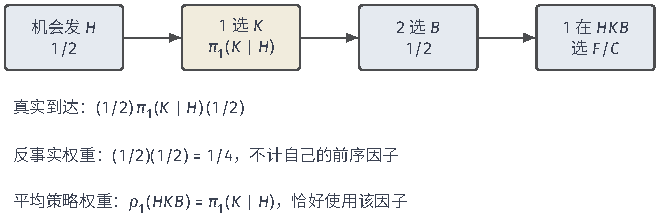
\includegraphics[width=111.651mm]{figures/10-reinforcement-learning/03-task-expansion-and-trustworthiness/tikz/rl-multi-agent-cfr-reach.pdf}
 \caption{高牌信息集$HKB$的真实与反事实到达权重。CFR价值保留机会和2的因子，去掉1的前序选择；用于汇总平均行为策略时，则需要1自身的前序因子。}
 \label{fig:rl-multi-agent-cfr-reach}
\end{figure}

CFR用这些价值在每个信息集运行局部遗憾匹配。一轮完整遍历先冻结$\bm\pi^{(k)}$，从根到叶计算到达因子，再从叶到根汇总式\eqref{eq:rl-multi-agent-cfr-value}。每个动作相对当前局部策略的价值差累加为
\[
 R_i^{(k)}(I,a)=R_i^{(k-1)}(I,a)+
        v_i^{\bm\pi^{(k)}}(I,a)-v_i^{\bm\pi^{(k)}}(I).
\]
遍历结束后，保存当前策略的平均权重，并统一由累计遗憾生成下一轮局部策略，避免同一次遍历混用新旧版本。

表\ref{tab:rl-multi-agent-cfr-round}以零遗憾和全部均匀策略开始，对隐藏牌游戏完成一轮上述计算。原策略期望收益为$J_1=1/8$，表中遗憾与概率均按各行所列动作顺序排列。

\begin{table}[htbp]
 \centering
 \begin{tabular}{@{}llll@{}}
 \toprule
 行动者与信息集 & 动作 & 本轮反事实遗憾 & 下一轮分布\\
 \midrule
 1，持$H$首次行动 & $(B,K)$ & $(3/16,-3/16)$ & $(1,0)$\\
 1，持$L$首次行动 & $(B,K)$ & $(3/16,-3/16)$ & $(1,0)$\\
 1，$HKB$ & $(F,C)$ & $(-3/8,3/8)$ & $(0,1)$\\
 1，$LKB$ & $(F,C)$ & $(1/8,-1/8)$ & $(1,0)$\\
 2，面对$B$ & $(F,C)$ & $(-1/4,1/4)$ & $(0,1)$\\
 2，面对$K$ & $(K,B)$ & $(-1/8,1/8)$ & $(0,1)$\\
 \bottomrule
 \end{tabular}
 \caption{隐藏牌游戏中全树遍历、同步更新的一轮CFR计算。2按自身收益$u_2=-u_1$计算遗憾，故不能直接复用1的收益符号。}
 \label{tab:rl-multi-agent-cfr-round}
\end{table}

以表中$HKB$这一行的计算为例，将终局收益乘上反事实权重，得$v_1(F)=-1/4$、$v_1(C)=1/2$；当前均匀策略值$v_1=1/8$，相减便得$(-3/8,3/8)$。2面对$B$时，高低牌各带对方与机会权重$1/4$，弃牌值为$-1/2$，跟注值为0，均匀当前值为$-1/4$，故只有跟注有正遗憾，下一轮必跟注。其余各行也可由已给的终局收益按同样步骤复算，无须补充游戏规则。

局部遗憾的用途不仅是改变信息集动作。在有限且完全回忆的博弈中，令$\mathcal I_i$为参与者$i$行动的信息集集合，这些局部量还给出完整策略偏离的上界：
\begin{equation}
 R_i^{(n)}
 \leq\sum_{I\in\mathcal I_i}
        \left[\max_a R_i^{(n)}(I,a)\right]_+,
 \label{eq:rl-multi-agent-cfr-bound}
\end{equation}
先用没有对手的两层树看清局部差额怎样相加。根节点选择Stop得到0，选择Go后再选Left或Right，收益分别为2和4。当前策略以$1/2$概率Go，到达下层后又以各$1/2$概率选Left或Right，故旧值为
\[
  \frac12\left(\frac12\,2+\frac12\,4\right)=1.5.
\]
考虑始终Go、随后始终Right的完整偏离，其收益为4。先只改根节点为Go、下层仍按旧策略，收益从1.5提高到3，增益为1.5；再把下层改为Right，收益从3提高到4，增益为1。两个差额相加得到
\[
  (3-1.5)+(4-3)=4-1.5=2.5.
\]
中间的3被消去，留下完整偏离的新旧收益差。下层增益按偏离策略到达下层的概率1计权，而不是按旧策略的到达概率$1/2$计权；否则会漏掉偏离后新增的访问。在博弈中还须保留对方与机会的到达权重，反事实价值正是先保存这部分，再与偏离者自身的到达因子配合。

式\eqref{eq:rl-multi-agent-cfr-bound}的左侧将式\eqref{eq:rl-multi-agent-external-regret}中的固定替代动作扩展为固定完整策略。完全回忆保证同一信息集具有相同的自身前序行动；递归分解收益差时，可以把固定偏离策略的自身到达因子提出信息集历史的求和。该因子介于0和1之间，累计局部增益因而由各信息集最大累计遗憾的正部控制。有限个信息集各自的遗憾增长为$o(n)$时，完整策略遗憾也为$o(n)$。这一结论只支持声明的完整策略偏离类，不能只凭局部观察到的动作收益就假定已取得所有信息集的反事实价值。原始CFR给出了该分解与局部遗憾界\scite{rl7-zinkevich2007}

获得这些局部量仍有成本。全树遍历的每轮计算随访问节点数增长，至少要保存$\sum_I|\mathsf A(I)|$个遗憾项及平均策略累加量。采样CFR可减少单轮访问节点，但需另给采样概率、支持条件，以及无偏反事实估计或相应误差界。任意舍弃罕见分支不能继承全遍历保证，深度近似也会引入拟合误差。

将遗憾界转为均衡保证时，要输出适当的平均策略，而非直接输出最后一轮。在完全回忆下，任取$h\in I$都具有相同的自身前序概率乘积，记为$\rho_i^{(k)}(I)$，不应在信息集内重复累加这一因子。按自身到达概率加权局部动作，得到平均行为策略
\begin{equation}
 \bar\pi_i^{(n)}(a\mid I)=
 \frac{\sum_{k=1}^{n}\rho_i^{(k)}(I)\pi_i^{(k)}(a\mid I)}
      {\sum_{k=1}^{n}\rho_i^{(k)}(I)}.
 \label{eq:rl-multi-agent-average-behavior}
\end{equation}
该比值来自自身序列实现概率的平均：分子对应到达$I$并选$a$的累加概率，分母对应到达$I$的累加概率，二者同时除以轮数后比值不变。逐层应用可恢复均匀抽取整套历史策略时的自身序列概率，而简单逐信息集算术平均通常不能。分母若为零，该信息集在平均实现计划中不可达，可规定任意合法分布，例如均匀分布。

例如，两个版本先过牌概率为0.1和0.9，在$HKB$处跟注概率为1和0。按自身到达加权的平均跟注率为0.1，而非算术平均0.5；它使“过牌再跟注”的自身序列概率为$0.5(0.1)=0.05$，正好等于$\tfrac12(0.1\cdot1+0.9\cdot0)$。若两人零和且各自平均外部遗憾至多$\varepsilon$，这些平均策略的总偏离间隙至多$2\varepsilon$，各人的偏离收益因此也至多$2\varepsilon$。第\ref{sec:rl-multi-agent-deviations}节将用零和消去证明这一结论；它不要求当前策略收敛，也不提供一般和Nash保证。

% Outline: 7.5.3
\Needspace{24\baselineskip}
\subsection{自我对弈与策略群体的迭代组织}
\label{sec:rl-multi-agent-population}

要让“针对历史响应”的学习真正发生，还得有一套训练对手的组织方式，否则很容易在几代之间丢掉重要的检验。比如一个“总让行”策略会被“总前进”克制；可若下一代只针对“总前进”训练、又把“总让行”彻底丢掉，就再也发现不了对手重新变温和时的机会——策略之间常常存在这种循环相克。

把“保留一批历史策略、再针对它们训练新策略”形式化，就得到策略库式的外循环。\term{策略空间响应预言机}（policy-space response oracles, PSRO）用策略库和库上博弈组织这一外循环。
令参与者$i$保存非空有限策略库$\mathcal P_i=\{\pi_i^1,\ldots,\pi_i^{K_i}\}$，其中$K_i\geq1$，每条策略均遵守原任务的观测、消息与行动权限。索引$k_i\in\{1,\ldots,K_i\}$指定一套完整策略。固定初态与交互协议后，库上收益表定义为
\[
 U_i(k_1,\ldots,k_m)
 =J_i(\pi_1^{k_1},\ldots,\pi_m^{k_m}).
\]
它是该组合的期望回报；由有限次对局估计得到的表另记$\widehat U_i$，并保存对局数、伙伴配对及采样随机性。因而估计误差和库中未包含的策略是两种不同限制。元混合策略$\sigma_i$是库索引上的概率分布，决定本回合使用哪套策略；它不同于环境中的$\pi_i(a_i\mid I_i)$，后者决定给定局部历史时采取哪个动作。通常先为一回合抽取一次索引，再执行整套行为策略，不在每一步重新换网络。

图\ref{fig:rl-multi-agent-psro}将库更新展开。先固定元对手$\bm\sigma_{-i}$，响应训练器对该索引分布平均回报，并优化
\[
 \mathbb E_{\bm k_{-i}\sim\bm\sigma_{-i}}
       J_i(\pi_i,\bm\pi_{-i}^{\bm k_{-i}}).
\]
响应器可调用第\ref{sec:rl-multi-agent-update}节的梯度或价值更新；元策略则可由零和求解器、遗憾更新或其他已规定的群体选择规则产生。获得$\hat\pi_i$后，估计其新增收益表项，将它加入库，再重新求元策略。原始PSRO组合的是近似响应训练与经验博弈求解，外循环并不要求响应器采用唯一的底层算法\scite{rl7-lanctot2017}

\Needspace{28\baselineskip}
实际系统未必完整计算上述元博弈，而会按任务选择群体维护方式。与第\ref{sec:rl-multi-agent-collection-plan}节的OpenAI Five版本抽样相比，AlphaStar的联赛训练（league training）设置主学习者和专门寻找其弱点的不同对手角色，再从保留的历史策略中选择训练对手\scite{rl7-vinyals2019}

OpenAI Five则主要维护共同训练的队伍，并混入历史版本对局以减少遗忘，并非为每个队员建立独立的均衡策略库。两种组织分别侧重多角色查找弱点和主训练中的历史检验。增加角色与库策略需要更多对局、存储和维护；这些机制安排了底层强化学习的经验来源，但系统规模本身不能证明已覆盖完整最佳响应。

\begin{figure}[htbp]
 \centering
 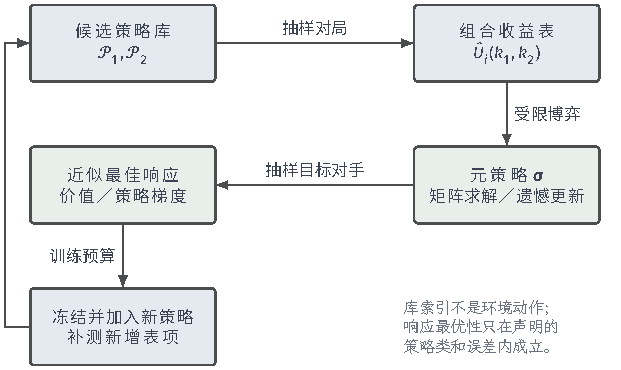
\includegraphics[width=105.184mm]{figures/10-reinforcement-learning/03-task-expansion-and-trustworthiness/tikz/rl-multi-agent-psro.pdf}
 \caption{PSRO的策略库外循环。收益表估计使用对局预算，响应训练使用交互与梯度预算；元策略规定响应对象，响应器规定底层更新计算。}
 \label{fig:rl-multi-agent-psro}
\end{figure}

策略库的限制可由三套抽象教学策略$\alpha,\beta,\chi$说明。以第一人的策略为行、第二人的策略为列，两人的索引都按$\alpha,\beta,\chi$排列，第一人的零和收益表为
\[
 \bm U=
 \begin{pmatrix}0&-1&1\\1&0&-1\\-1&1&0\end{pmatrix}.
\]
从表中可见，$\beta$必胜$\alpha$，$\chi$又必胜$\beta$，没有一套最强纯策略。若双方库只有$\{\alpha,\beta\}$，元解都选$\beta$，库内没有获利偏离；库外的$\chi$却能取得1。加入全部三套策略后，均匀混合使各行收益都为0。这区分了击败当前对手、求解已有收益表中的均衡和覆盖所有可能响应：前两项成立，第三项仍可能失败。

若双方库各有$K$套策略，每格评价$E$局，完整收益表就需$K^2E$场；增加一行一列还须补测相关组合，多方全组合表的项数则为$\prod_iK_i$。响应网络、检查点及响应训练与收益估计的对局记录也占用预算。收益估计误差、响应搜索误差及库外策略都会使元博弈与完整博弈不同，因而受限元解不能单独认证完整博弈不可利用。

% Outline: 7.5.4
\subsection{学习动态的稳定性与保证对象}
\label{sec:rl-multi-agent-stability}

更新怎么算、对谁响应、训练群体如何组织，三者合起来决定了学习动态，因此任何“会收敛/很稳定”的声明都必须对应这一完整组合，换掉其中一个模块结论就可能失效——例如把精确的表格遗憾更新换成误差不受控的神经网络近似，原来的收敛定理就不再适用。表\ref{tab:rl-multi-agent-dynamics}列出各组合实际能保证的输出对象。

\begin{table*}[htbp]
 \centering
 \begin{tabularx}{\linewidth}{@{}l l l >{\raggedright\arraybackslash}X >{\raggedright\arraybackslash}X >{\raggedright\arraybackslash}X@{}}
 \toprule
 更新接口 & 响应规则 & 训练群体 & 当前策略表现 & 平均策略表现 & 保证条件\\
 \midrule
 梯度 & 同时追随 & 当前双方 & 可旋转或发散 & 局部改进不足以保证平均间隙下降 & 另需步长、博弈与算子条件\\
 精确响应 & 历史平均 & 历史策略 & 可持续变化 & 有限两人零和的经典虚构博弈平均可收敛 & 精确响应、完整有限博弈；近似误差另计\\
 局部遗憾 & 同步CFR & 当前与平均 & 不要求收敛 & 适当平均的零和间隙受遗憾界控制 & 有限、完全回忆、正确价值或采样误差控制\\
 梯度响应器 & 元策略响应 & PSRO策略库 & 新响应未必稳健 & 元混合只解受限经验博弈 & 收益表误差、响应误差及策略类限制均需报告\\
 \bottomrule
 \end{tabularx}
 \caption{更新计算、响应规则和群体组织共同确定的保证。当前策略、平均行为策略与库上的元混合策略对应不同输出，应分别报告。}
 \label{tab:rl-multi-agent-dynamics}
\end{table*}

为直观区分这些输出，图\ref{fig:rl-multi-agent-stability}沿用匹配硬币和同一初值，计算交替更新轨迹。固定当前$(p,q)$，两人分别求最佳响应得到总单方偏离间隙
$g(p,q)=|2p-1|+|2q-1|$；检验平均策略时，则代入历轮$p,q$的均值。图中另按固定动作在整段历史上的错失收益计算
\[
 \frac1n\max\!\left\{0,\
 \left|\sum_k(2q^{(k)}-1)\right|-\sum_k u^{(k)},\
 \left|\sum_k(2p^{(k)}-1)\right|+\sum_k u^{(k)}\right\},
\]
这是两人累计平均外部遗憾正部中的较大值，其中绝对值来自比较两个固定纯动作。三条曲线使用同一序列，当前间隙波动时，平均间隙仍可下降。有限步长下遗憾还可能保留偏差，因此图形只能展示所给递推的有限轮次结果，不能据形状断言任意精度收敛。

\begin{figure}[htbp]
 \centering
 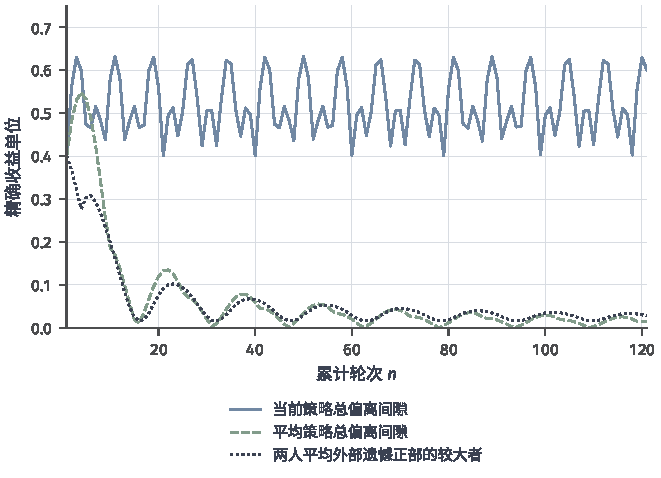
\includegraphics[width=112.000mm]{figures/10-reinforcement-learning/03-task-expansion-and-trustworthiness/matplotlib/rl-multi-agent-stability.pdf}
 \caption{同一交替梯度序列的三种检验量。当前间隙、平均策略间隙与累计平均遗憾均由精确矩阵收益计算，图源保留递推及统计公式，不代表学习基准的实验成绩。}
 \label{fig:rl-multi-agent-stability}
\end{figure}

判断保证能否沿用，需要定位每项误差作用的位置：评论家和采样误差改变收益或梯度估计，近似响应误差改变每轮与最佳响应的比较，共同学习改变下一批交互记录的分布，不完全回忆破坏信息集分解，库外策略则不在元博弈的比较类中。低外部遗憾要进一步控制平均边际策略的Nash间隙，须利用两人零和的收益抵消。一般和中通常只能得到保留相关性的联合经验分布结论，不能按相同证明推出平均独立策略达到Nash均衡。

即便阶段博弈做到了无悔，改变早先动作还会改变后面访问哪些状态。只在已访问位置比较动作，不能控制新策略将到达的位置及其后续回报。需要把后继价值向前传播，同时为未充分探索的位置保留余量。\term{V学习}（V-learning）把状态价值估计、探索与各人的局部对抗老虎机连接起来，并用训练历史构造完整的策略输出。

考虑正整数$H$和有限状态、行动空间，所有参与者在阶段$t=0,\ldots,H-1$行动前共同看到当前状态。每回合都从同一初态生成规则重新开始，转移与奖励规律可以随阶段$t$变化，但在训练回合间固定；每步奖励满足$r_{i,t}\in[0,1]$，第$H$步后终止。这里评价不折扣的整回合回报$\mathbb E\sum_{t=0}^{H-1}r_{i,t}$，与前面的无限折扣目标分开。因此，阶段$t$之后最多还有$H-t$单位回报；这一已知上界正是初始化与截断的依据。

每个参与者$i$为每个$(s,t)$保存状态价值$V_{i,t}(s)$、访问计数和一个只选择自身动作的\term{对抗老虎机}（adversarial bandit）子程序。第~\ref{sec:rl-learning-contextual}~节已说明，它用所选动作的反馈调整动作分布，以应对随历史变化的损失；此处损失会随其他人的学习而变化，不要求环境中另有恶意攻击者。价值初值为$H-t$，终端价值$V_{i,H}=0$。在$(s,t)$第$n\geq1$次访问、取得$r_i$和$s'$后，更新为
\begin{equation}
 \begin{aligned}
  \alpha_n&=\frac{H+1}{H+n},\\
  \widetilde V_{i,t}(s)&\leftarrow
      (1-\alpha_n)\widetilde V_{i,t}(s)
      +\alpha_n\bigl[r_i+V_{i,t+1}(s')+b_{i,n}\bigr],\\
  V_{i,t}(s)&\leftarrow\min\{H-t,\widetilde V_{i,t}(s)\}.
 \end{aligned}
 \label{eq:rl-multi-agent-v-learning}
\end{equation}
$\widetilde V$同样从$H-t$初始化，$b_{i,n}\geq0$是按遗憾与采样误差选取的探索余量；它使未充分采样的后果保持乐观，截断则保留已知回报上限。访问次数$n$决定更新权重，并非环境时刻$t$。局部动作子程序收到已选动作及损失$(H-r_i-V_{i,t+1}(s'))/H$，再更新自身动作分布。由于$0\leq r_i+V_{i,t+1}(s')\leq H-t\leq H$，该损失在$[0,1]$内；未选动作的损失并未全部观测，须由带相应加权遗憾保证的bandit更新处理。价值表因而不必按联合动作展开，但每个人仍需保存自己的动作概率与历史策略。

式~\eqref{eq:rl-multi-agent-v-learning}~的更新权重也规定了策略怎样混合。对已有$n$次访问的位置，第$j$次访问的历史权重为
\[
 \omega_{n,j}=\alpha_j\prod_{\ell=j+1}^{n}(1-\alpha_\ell),
 \qquad j=1,\ldots,n,\qquad\sum_{j=1}^n\omega_{n,j}=1.
\]
例如$H=2,n=2$时，$\alpha_1=1,\alpha_2=3/4$，历史权重为$(1/4,3/4)$；两份局部策略选择某动作的概率若为0.2和0.8，该次混合概率就是0.65，既不是最后一份策略的0.8，也不是均匀平均的0.5。这只演示一次局部混合。完整输出先均匀抽取训练回合索引，在每个到达的状态—时刻对，再按该索引之前的访问记录和上述权重抽取历史回合，按该回合的策略快照选择当前动作，并把抽到的索引带入下一步继续回退；未访问位置需保留初始化策略。必须保存相应计数与策略快照，不能将这一递归协议换成均匀抽取某一回合策略后整局不变。该输出一般依赖历史，不是只读取当前状态的最后一轮策略。

均衡目标决定局部遗憾和联合输出的要求。两人零和时，各人独立执行这一历史输出协议，所得乘积策略可有近似Nash保证。多人一般和时，加权外部遗憾控制对应近似CCE；若改用控制动作替换映射的加权交换遗憾子程序，则可取得近似CE。一般和的联合输出还须在执行前共享一次随机种子，同步各步抽取的历史索引，以保留所需相关性，各人的动作仍由各自策略产生。训练分散执行，并不意味着执行时可以删掉这个公共随机协议。

零和任务可按已知奖励界作正尺度变换与常数平移，采用$r_{2,t}=1-r_{1,t}$的单位区间常和计分。固定$H$时，这种等价编码保留最佳响应与均衡策略，收益误差则须按新旧尺度换算。

在上述有限表格、共同可见状态与单位区间奖励条件下，采用原论文给出的加权正则化跟随领头者（follow-the-regularized-leader, FTRL）子程序，按累计损失估计与正则项选择下一动作分布，并配合相应探索余量及完整历史输出协议。令$n_S=|S|$、$n_{A,\max}=\max_i|\mathsf A_i|$。对$\varepsilon>0$和$\delta\in(0,1)$，两人零和的$\varepsilon$-Nash与一般和的$\varepsilon$-CCE都可在
$\widetilde O(H^5n_Sn_{A,\max}/\varepsilon^2)$个训练回合后以至少$1-\delta$的概率取得；加权交换遗憾版本取得$\varepsilon$-CE的对应量级为
$\widetilde O(H^5n_Sn_{A,\max}^2/\varepsilon^2)$。这里$\varepsilon$按归一化逐步奖励的整回合收益衡量，$\widetilde O$隐藏包括失败概率和参与者数在内的对数因子，一回合至多$H$个环境步。动作规模由联合空间的乘积变为最大单人动作数，是这类结论的关键；它没有保证最后一次策略收敛，也不能直接推广到局部观测、任意神经近似或随意选取的探索余量。具体子程序与输出条件见原论文算法1、3及定理5--7\scite{rl7-jin2021vlearning}

从训练对手表现到元博弈，再到完整策略空间的最佳响应，所需验证范围逐步扩大，训练却未必自然完成这些检验。恶意通信、对抗攻击和安全约束还会改变行为要求，第\ref{chap:rl-trustworthy}章另作讨论。即便当前训练曲线稳定，也不能据此获得这些新目标的保证。

% Outline: 7.6
\section{多智能体的参与者变化适配}
\label{sec:rl-multi-agent-adaptation}

前面所有讨论都默认参与者的人数、伙伴和接口是固定的。部署时这些前提经常变化：机器人团队可能临时增加人手，合作伙伴可能换成一套从未配合过的陌生策略，竞争者也可能采用全新的行为机制。这些是性质不同的适配问题，可以沿用第\ref{chap:rl-transfer}章的训练分布、留出条件和适应预算框架，但必须把“参与者如何变化”明确写进去。跨规模、跨伙伴、跨对手分别改变的条件不同，不能因为在一种变化下协调成功，就同时声称具备了另外两种适配能力。

% Outline: 7.6.1
\subsection{参与者规模变化下的跨规模适配}
\label{sec:rl-multi-agent-scale}

先看人数变化。参与者增加时，原来为固定人数设计的策略可能连输入格式和协作约定都无法复用。例如两人网络若用固定槽位拼接“对方的位置”，就没有放入第三人的槽位；“1 先走、2 后走”的约定也没有规定第三人何时行动。

连续控制还须说明“一个参与者”控制什么。分解式多智能体集中策略梯度（factored multi-agent centralised policy gradients, FACMAC）所用多智能体MuJoCo任务按关节组控制同一系统；更换分组或观测半径会改变各人的动作集合和可见观测范围。此时即使人数相同，任务接口也可能不同，不能只比较参与者数量\scite{rl7-peng2021facmac}

对角色与动作编码相容的参与者，若编号只用于登记身份，重编号就不应改变各物理参与者的决策。把$m$人的动作前可见特征排成$\bm X\in\mathbb R^{m\times d}$，每行对应一人；邻接矩阵$\bm B\in\mathbb R^{m\times m}$记录可用的交互边。固定参数的图策略$F(\bm X,\bm B)$逐行给出各人的动作分布参数，各行使用同一动作编码。令$\bm M$为$m\times m$置换矩阵，同时重排特征行与邻接矩阵的行、列。若
\[
 F(\bm M\bm X,\bm M\bm B\bm M^\top)=\bm M F(\bm X,\bm B),
\]
就具有\term{置换等变性}（permutation equivariance）：先重编号再求策略，等于先求策略再相应重排结果。例如交换1、2两人的编号后，原1对应的策略分布应出现在新2的位置，而不是强迫两人使用相同动作。角色特征也必须随物理参与者一起重排。这是消除任意编号影响的结构要求；能够处理变长有序列表的策略不必满足它，因此变长计算与重编号对称是不同性质。

共享的邻域消息函数与不依赖邻居排列的聚合器，可以构造这种图策略：
\[
 \bm z_i=\operatorname{Agg}_{j\in\mathcal N_i}
           \phi(I_i,I_j,e_i,e_j),\qquad
 \pi_i(\cdot)=f_{\bm\theta}(I_i,e_i,\bm z_i),
\]
其中$\mathcal N_i$为$i$的邻居集合，$\phi$将一对参与者的局部特征映为消息向量，$\bm z_i$为聚合结果；此处$e_i$表示可见角色，不是任意编号，$\operatorname{Agg}$可取不依赖邻居排列的求和、均值或邻居集合上归一化的注意力。空邻域须规定合法输出，例如零向量，才能在所有图上计算策略；按身份槽位拼接一般不具有上述性质。图\ref{fig:rl-multi-agent-graph}展示同一物理图重编号后的对应。部署聚合只能使用本轮动作前实际收到的邻居消息及协议允许共享的字段，不能因图结构可写而假定邻居历史全部可见。

\begin{figure*}[htbp]
 \centering
 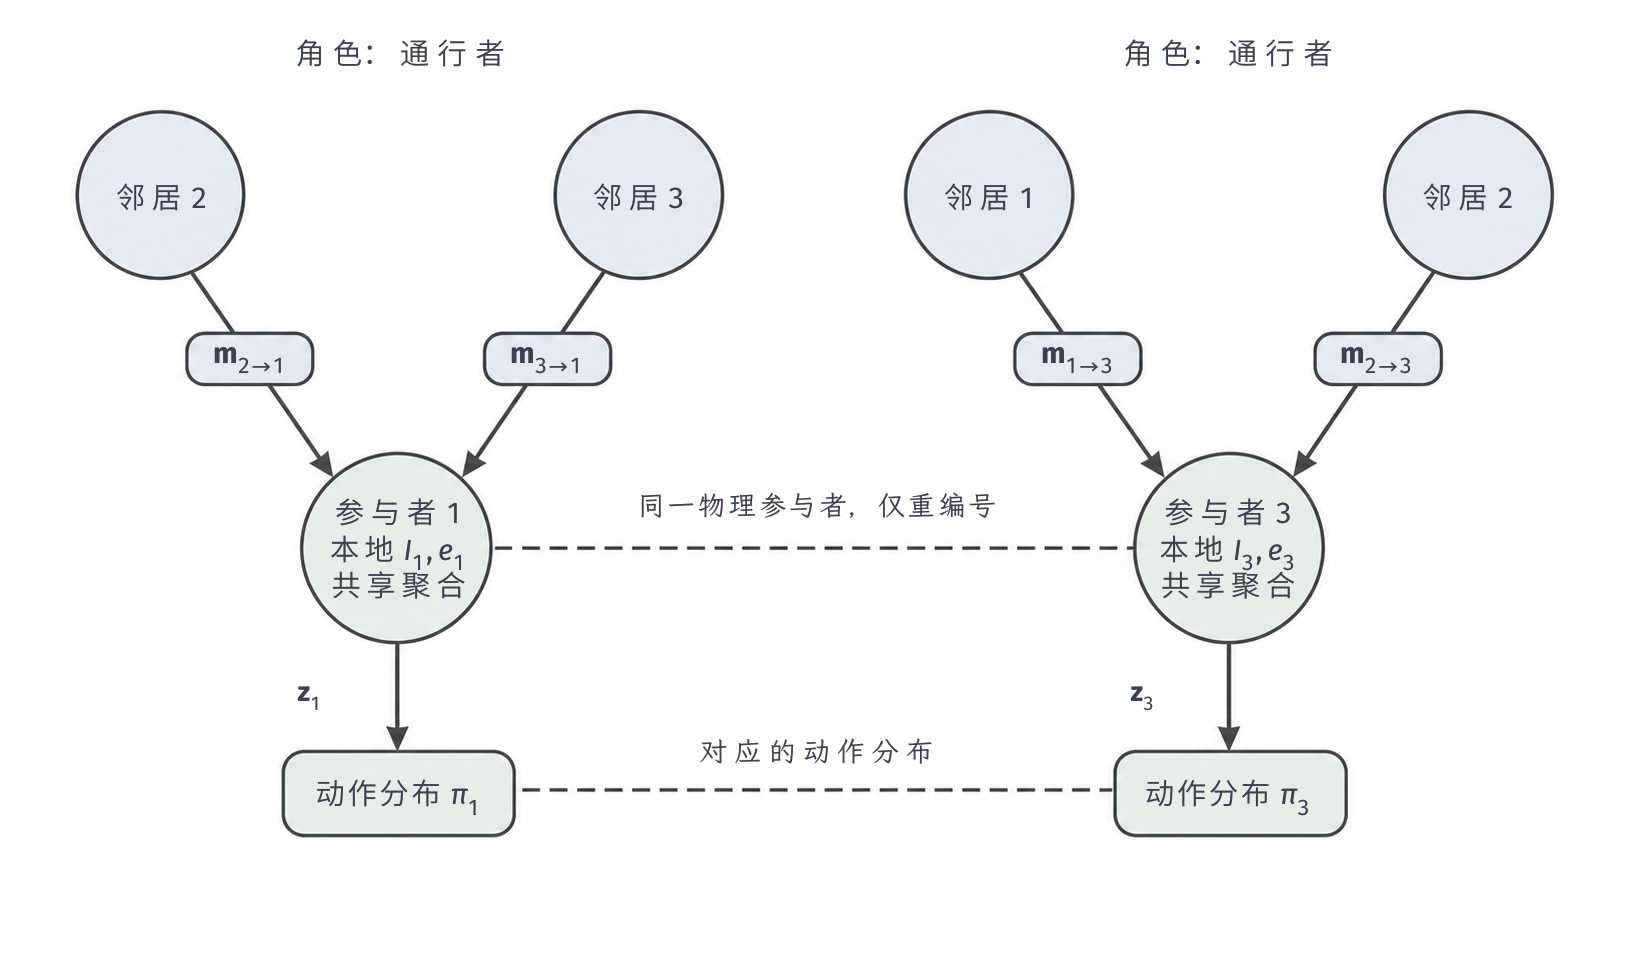
\includegraphics[width=157.400mm]{figures/10-reinforcement-learning/03-task-expansion-and-trustworthiness/generated/rl-multi-agent-graph/figure.png}
 \caption{共享邻域聚合对重编号的响应。实线把邻居消息送至本地主体，再形成动作分布；左右图仅重排同一物理节点的编号。横向虚线连接重编号前后的同一主体及相应动作分布，不是额外通信边；通行任务不变。}
 \label{fig:rl-multi-agent-graph}
\end{figure*}

当邻居很多时，逐个建模“我和每个邻居的交互”成本太高，一个自然的近似是只看群体或邻域的平均行为，把所有他人的联合影响压缩成一个“平均动作”。平均场多智能体强化学习（mean field multi-agent reinforcement learning）
\[
 \bar{\bm a}_{-i,t}
 =|\mathcal N_i|^{-1}\sum_{j\in\mathcal N_i}\bm e(a_{j,t}),
\]
其中$\bm e(a_{j,t})$为动作独热向量，求平均后得到时刻$t$实际执行后的邻域动作频率。空邻域另约定$\bar{\bm a}_{-i,t}=\bm0$，这只是无邻居标记，不是概率分布。同时行动时，参与者提交$a_{i,t}$之前不能读取尚未产生的$\bar{\bm a}_{-i,t}$；执行策略必须改用事前可得的估计$\widehat{\bar{\bm a}}_{-i,t}$。协议可以规定它由上一时刻已观察的均值、邻居策略预测，或同步求解的自洽平均场得到，但训练和评价须固定同一种构造；若通信直接公开本轮意图动作，则应把这项额外权限写入历史。已完成的联合转移可用实际$\bar{\bm a}_{-i,t}$训练评论家，而下一步TD目标中的聚合量须按同一事前规则构造$\widehat{\bar{\bm a}}_{-i,t+1}$。学习器据此将聚合行为作为$Q_i(I_i,a_i,\bar{\bm a}_{-i})$的条件。若后继目标只把事前点估计代入非线性评论家，这里采用的是点代入近似；若要计算对未来实际均值的条件期望，还需对其预测分布采样或积分。训练与评价应保留同一近似口径。原始平均场方法沿这一路线给出Q学习和行动者—评论家机制\scite{rl7-yang2018meanfield}

共享图策略可继续由联合轨迹和团队目标训练，并在训练中覆盖不同图与规模，执行时按当前邻域组装输入。令$E_G$为图边集，每轮沿各边计算消息需要$O(|E_G|)$次函数调用，传递$L$轮则乘$L$；这是固定单条消息计算结构时的调用数，不是整个网络的运行时间。网络能接受变长输入，只解决计算可定义的问题，不保证新人数$m$下回报不降。聚合方式也决定哪些局部特征差别仍可区分：求和随人数变化，均值可能丢掉邻居数量，即便置换等变也可能需要显式计数或密度特征。

平均场近似还要求个体影响较弱、聚合量足以描述交互，仅人数多并不充分。窄通道中一个关键参与者就能完全堵塞，平均前进率却未必指出谁占据瓶颈。异质角色、强配合或拓扑突变也可能使聚合量不足，所以近似有效性仍须在留出规模与交互条件下检验。

% Outline: 7.6.2
\subsection{未见合作者条件下的零样本协调与在线适配}
\label{sec:rl-multi-agent-new-partners}

换伙伴和换人数是两回事：人数不变、只换一个合作伙伴时，最容易出问题的不是技能，而是双方默认的协调约定是否兼容。

Overcooked的共享烹饪任务中也有这种区别。同一厨房下，与共同训练的伙伴完成分工，不代表能与新伙伴保持同样配合；评价须给出伙伴来源，并规定双方是否允许适应\scite{rl7-carroll2019}

先按第\ref{sec:rl-transfer-budget}节区分零样本与适应预算。本章对\term{零样本协调}（zero-shot coordination）采用同样的严格预算口径：不使用新伙伴反馈作伙伴特定的参数更新、记忆适应、类型辨识或模型选择，但可读取已给角色、约定及正常控制所需的观测。在给定任务和伙伴模型下估计当前位置，仍属普通状态估计；利用伙伴动作或回报改变对其行为类型的判断，则已发生适应。即使这一判断只在首回合内更新、网络参数始终固定，也不能按本章口径称为零样本。

文献中的zero-shot coordination有时主要强调测试伙伴未与当前策略共同训练；是否允许首回合内利用伙伴反馈，还须读取具体协议。将这些结果按本章分类时，应按实际反馈、记忆重置与参数更新权限归类。

\term{临时团队协作}（ad hoc teamwork）研究未预先共同训练或充分协调的新队伍，协议可以允许交互辨识和伙伴适配。为确定其可行策略，实验须说明是否共享左右约定、能否通信、角色是否可见、允许试探几步，以及试探失败的代价。任务名称并不自动提供这些权限。

机制选择须与可读任务约定、伙伴类型线索和交互历史对应。扩大训练伙伴群体要有多类伙伴可供交互，处理对称性要知道哪些变换保持任务不变，伙伴条件策略要有部署时可见的类型线索，在线信念更新则要有能区分类型的历史。Other-Play利用所给任务对称性，减少策略对某次自我对弈任意约定的依赖；作用范围仍由该对称性与协调条件限定，不能保证兼容任意未知伙伴\scite{rl7-hu2020otherplay}

一种在线协议先冻结基础策略与类型模型，在前$B$步用获准动作或消息收集证据，再按第\ref{sec:rl-multi-agent-opponent-model}节更新信念，以伙伴条件价值选动作。若还允许梯度适配，须另计更新次数和目标伙伴交互训练记录的来源。报告应区分零样本、仅记忆或信念适应、参数适应，并说明回合内及跨回合的记忆保留。适应后评价可继续估计物理状态，但只要反馈仍修正伙伴类型，适应过程就没有结束；若两者无法分离，也应据实计入协议。交互数量增加不保证类型可辨识，证据不足时仍可能无法区分伙伴。

最后，分工还受观测、历史和角色信号的对称性限制。双方若使用同一确定性策略、取得同一历史，又没有身份、方位或指定不同角色的公共信号，所选动作就相同，无法保证恰好一人前进。独立随机化提供打破对称的机会，却不能保证本轮形成指定分工。合法公共角色信号能改变可行策略集合，因此使用它时须在评价协议中明示。

% Outline: 7.6.3
\subsection{未见竞争者条件下的策略适应}
\label{sec:rl-multi-agent-new-opponents}

面对新竞争者，还要在“针对已知弱点尽量榨取收益”和“对手一变也不至于被反制”之间权衡。

对手条件策略可以先在训练群体中学习行为表示，部署时据可见动作、回合结果或消息更新类型信念，再选择响应。优化目标可以是给定对手分布下的收益，也可以另加已知策略类中的最坏情形限制；比较适应速度前必须先说清使用哪种目标。表\ref{tab:rl-multi-agent-opponent-adaptation}列出相应比较对象，并区分固定对手与随自身行为响应的对手。

\begin{table}[htbp]
 \centering
 \begin{tabularx}{\linewidth}{@{}l >{\raggedright\arraybackslash}X >{\raggedright\arraybackslash}X@{}}
 \toprule
 问题 & 对手、历史及允许更新 & 比较对象\\
 \midrule
 固定对手最佳响应 & 目标固定；可交互观测；按给定预算更新 & 同一对手下可行最佳响应收益\\
 群体内适应 & 见过类型的新抽样；允许历史辨识或少量更新 & 同预算的群体条件基线及零样本策略\\
 跨对手泛化 & 未见行为类型；历史与反馈权限明确 & 留出类型的平均、尾部及最坏已测收益\\
 反应型对手适应 & 对方可随自身行为改变；响应历史需记录 & 声明响应协议下的序贯收益，非固定对手值\\
 \bottomrule
 \end{tabularx}
 \caption{对手适应的目标与可用证据。需同时给出类型留出、记录采集与访问权限和比较对象；同一策略只更换随机种子并未构成类型留出。}
 \label{tab:rl-multi-agent-opponent-adaptation}
\end{table}

例如，规定20场探测再评价100场时，还须确定探测是否计分、记忆是否重置、梯度步上限，以及对手在全部120场中是否保持不变；这些数字仅定义教学预算。响应训练使用的对局不能同时充当独立测试。对手若先以温和行为诱导信念、随后切换，或在探测中继续学习，固定类型模型就可能不适用。此时须按第\ref{sec:rl-multi-agent-response-model}节重新规定响应机制，不能保留固定类型识别的保证。

% Outline: 7.6.4
\subsection{参与者变化适配的泛化与扩展边界}
\label{sec:rl-multi-agent-generalization}

无论测试跨规模、跨伙伴还是跨对手的适配，都应先声明究竟变化了哪个因素，并据此划分训练、验证与测试的参与者及交互记录；把多种变化混在同一批“新环境”测试里，成功或失败都无法归因。

\begin{table}[htbp]
 \centering
 \begin{tabularx}{\linewidth}{@{}l >{\raggedright\arraybackslash}X >{\raggedright\arraybackslash}X@{}}
 \toprule
 变化因素 & 可声明的留出方式 & 必须控制或记录\\
 \midrule
 数量与密度 & 训练2至4人，测试6人等独立设定 & 通道容量、拥挤度、邻域大小，不能只改$m$\\
 身份与组合 & 已见类型的新排列、新搭配 & 角色是否同构；是否共享编号约定\\
 合作者或对手类型 & 留出训练流程、策略家族或行为机制 & 零样本／适应预算；伙伴是否继续学习\\
 收益关系 & 固定关系内的新参数，或另测关系改变 & 团队转竞争已改变目标，不能仅称身份泛化\\
 通信与拓扑 & 留出图、延迟、带宽或接收范围 & 部署消息是否可得；公共信号是否保留\\
 \bottomrule
 \end{tabularx}
 \caption{参与者变化的留出方式与控制条件。支持内的新搭配和未见行为类型不是同一种测试，其覆盖与辨识要求不同。}
 \label{tab:rl-multi-agent-splits}
\end{table}

同一批伙伴更换环境种子，只检验给定伙伴下的运行随机性；同一策略更换编号，至多检验身份依赖。若同时改变人数、角色、奖励和通信，失败不能单独归因于规模，成功也难以辨认是哪项适配有效。因此应先作单因素留出，再评价明确的组合变化，结论范围始终受实际留出因素限定。

% Outline: 7.7
\section{多智能体的行为评价和验证}
\label{sec:rl-multi-agent-evaluation}

最后是评价。多智能体系统的“好”有多个互不替代的侧面，必须分别检验：策略取得了多高的收益？是否满足选定的行为标准（有没有单方面偏离的动机）？能否和声明范围内的新伙伴、新对手正常交互？又花费了多少资源？基准回报说明任务表现，偏离搜索检查稳定性，交叉配对检查约定是否兼容，资源统计说明代价。把这些量压成一个无条件的单一排名，会丢掉各自的验证范围。

% Outline: 7.7.1
\subsection{共同评价目标下的效用、福利与公平评价}
\label{sec:rl-multi-agent-welfare}

评价收益时应先回到各方原本的目标，不能用一个总分掩盖分配差异。

例如，教学结果$(10,0)$与$(5,5)$总收益都为10，最小收益分别为0和5，个体收益的总体方差分别为25和0。若第一种结果总由同一人承担成本，只报团队总分便看不到差异；若角色按公平规则轮换，还需区分单回合和长期分配。实际评价应至少报告均值、分布与失败率，并定义失败究竟是碰撞、超时还是某人的任务未完成。

指标还须对应具体任务接口，表\ref{tab:rl-multi-agent-benchmarks}为此区分环境库中的任务。例如，星际争霸多智能体挑战（StarCraft multi-agent challenge, SMAC）考察局部观测下的团队微操，即多个受控单位分别选择移动、攻击等战斗动作；地图和敌人脚本共同决定难度与胜率含义，不能只写环境库名称来确定评价条件\scite{rl7-samvelyan2019}。表中的MPE指多智能体粒子环境（multi-agent particle environment），其收益、观测与通信同样由具体任务配置决定。

\begin{table*}[t]
 \centering
 \begin{tabularx}{\linewidth}{@{}l >{\raggedright\arraybackslash}X >{\raggedright\arraybackslash}X >{\raggedright\arraybackslash}X >{\raggedright\arraybackslash}X@{}}
 \toprule
 具体接口 & 合作或竞争结构 & 可用观测 & 通信条件 & 主要指标\\
 \midrule
 SMAC，3m & 三个受控单位合作，对抗脚本敌人 & 各自视野内的单位特征；训练可给全局状态 & 原任务无额外学习消息，新增须声明 & 地图胜率、回报、超时率\\
 MPE，simple\_spread & 多个体覆盖地标；局部碰撞项与共享项比例需指定 & 自身及其他实体的配置相关特征 & 此任务的静默体无消息；不能外推至其他MPE任务 & 覆盖距离、碰撞及所定奖励\\
 Overcooked，cramped\_room & 两人完成共享烹饪与交付任务 & 厨房布局、物品及参与者状态的指定编码 & 原动作接口无自由语言频道 & 交付数、团队回报、分工及等待\\
 PettingZoo，rps & 两人石头剪刀布，零和 & 本轮选择在双方提交前相互隐藏 & 无显式消息；AEC调用次序不等于看见先行动作 & 各自收益及偏离间隙\\
 多智能体MuJoCo，分组HalfCheetah & 不同关节组共同控制同一系统 & 分组关节特征及指定观测半径 & 消息或额外关节状态需另列 & 回报、预先定义的失稳事件率、推理时延\\
 \bottomrule
 \end{tabularx}
 \caption{具体任务接口的收益、可见观测与评价指标。复现还须固定软件版本、地图、观测包装器、奖励配置及回合上限，不能只指定环境库。}
 \label{tab:rl-multi-agent-benchmarks}
\end{table*}

多智能体粒子环境中的收益和通信配置因任务而异，一个任务采用静默动作不能说明整个环境族都无通信。Overcooked还应将共同训练伙伴与新伙伴的结果分开，才能对应第\ref{sec:rl-multi-agent-new-partners}节所区分的协调能力。

PettingZoo石头剪刀布的检验重点包括屏蔽对方本轮尚未提交的动作。调用程序可以先保存一人的动作，另一人的策略却不能据此选择本轮动作；这正是第\ref{sec:rl-multi-agent-information}节所要求的调用顺序与可见时序分离。

连续控制则须按第\ref{sec:rl-multi-agent-scale}节记录关节分组和每组可见的关节状态，仅写“MuJoCo”不能确定控制接口。改变人数或观测半径也会改变协调条件，相应结果不能当作同一问题直接比较。

不同接口的动作粒度、回合长度和奖励尺度不同，原始分数不能直接求和。评价时提供给行动者的观测、消息及送达时序须与部署一致，不应额外提供全局状态或免费通信。若训练使用奖励塑形，宜同时给出原任务指标与实际优化回报，以区分塑形目标提高和任务确实完成。

% Outline: 7.7.2
\subsection{行为标准下的偏离收益、遗憾与可利用性验证}
\label{sec:rl-multi-agent-deviations}

平均回报高，并不代表这个局面是稳定的——也许某个参与者稍作改变就能获得更大好处。因此还要专门检查单方偏离标准：固定其他人的完整策略，搜索$i$在相同的行动前观测、历史与消息权限下能找到的最好替代策略，并比较两者回报。
\[
 \delta_i(\bm\pi)=
 \sup_{\pi_i'\in\Pi_i}J_i(\pi_i',\bm\pi_{-i})-J_i(\bm\pi).
\]
比较类$\Pi_i$必须保留原观测、消息与行动权限，并含当前$\pi_i$；不作改变就是其中一种选择，故$\delta_i\geq0$。两人零和时，本章将双方偏离收益相加，记总间隙$g=\delta_1+\delta_2$。部分软件以$g/2$称为可利用性，报告中要标明采用的约定。

匹配硬币中取$p=0.7,q=0.4$，当前$u_1=-0.08$。固定$q$，1改为第二动作得0.2，偏离收益$\delta_1=0.28$；固定$p$，2改为第二动作使1得$-0.4$，自身从0.08升到0.4，故$\delta_2=0.32$。总间隙为0.6，按半间隙约定为0.3。只对均匀对手测得零回报，无法发现这种能被针对性响应利用的偏好。

第\ref{sec:rl-multi-agent-mutual-learning}节介绍了产生低遗憾的机制。下面从遗憾定义推导可验证的结论，并保留其中的联合分布与零和条件。

固定正整数$n$与$\varepsilon\geq0$，将各人非空有限动作集上的固定有限阶段博弈重复$n$轮，实际联合动作为$\bm a^{(k)}$，按联合动作频率定义经验分布
$\hat q_n(\bm a)=n^{-1}\sum_{k=1}^n\mathbf1\{\bm a^{(k)}=\bm a\}$。
若每个人对每个固定替代动作的累计外部遗憾都不超过$n\varepsilon$，则$\hat q_n$满足$\varepsilon$粗相关均衡约束。若进一步对每对动作$a_i,b_i$，仅在实际选$a_i$的轮次改用$b_i$的内部遗憾满足
\[
 \sum_{k=1}^n\mathbf1\{a_i^{(k)}=a_i\}
 [u_i(b_i,\bm a_{-i}^{(k)})-u_i(\bm a^{(k)})]
 \leq n\varepsilon,
\]
则$\hat q_n$满足每对动作的未条件化$\varepsilon$相关均衡偏离约束。
这个结论按联合动作频率合并遗憾和：外部遗憾对应事前固定偏离，内部遗憾只保留实际建议为$a_i$的轮次，因此对应未条件化的建议替换。两者都保留联合频率，不要求各人的动作独立；它们用于检验重复交互的经验行为标准，不能单凭它们认证最后一轮策略已经收敛。

若改为评价收到$a_i$后的条件收益，需要两边同时除以建议概率$\hat q_{n,i}(a_i)$，条件误差界成为$\varepsilon/\hat q_{n,i}(a_i)$，对罕见建议可能很大。零概率建议不需定义条件期望。若允许同时替换多个建议，逐对约束的误差相加还会累积，不能直接把每对动作的$\varepsilon$解释为任意交换映射的同一界。

保留联合频率是结论成立的关键。协调约定$(L,L)$和$(R,R)$各占一半时，经验分布从不失配，但各人边缘都是均匀分布；取边缘乘积就出现$1/2$的失配概率。一般和的低遗憾控制前一种相关分布，通常不控制后一种独立边际平均策略的Nash偏离。

固定正整数$n,p,q$与$\varepsilon_1,\varepsilon_2\geq0$，考虑有限两人零和收益矩阵$\bm A\in\mathbb R^{p\times q}$。第$k$轮采用混合策略$\bm x^{(k)}\in\Delta_p,\bm y^{(k)}\in\Delta_q$，候选集合为全部行、列动作概率分布。若按期望收益计算的双方累计外部遗憾分别不超过$n\varepsilon_1,n\varepsilon_2$，则各自平均策略
$\bar{\bm x}=n^{-1}\sum_{k=1}^n\bm x^{(k)}$、$\bar{\bm y}=n^{-1}\sum_{k=1}^n\bm y^{(k)}$满足
\[
 \max_{\bm x\in\Delta_p}\bm x^\top\bm A\bar{\bm y}
 -\min_{\bm y\in\Delta_q}\bar{\bm x}^\top\bm A\bm y
 \leq\varepsilon_1+\varepsilon_2.
\]
左侧是这对平均策略的总单方偏离间隙，用于把双方无悔证据转成平均策略的均衡误差。收益对各方混合策略的线性性允许按轮次平均，而两人零和使双方遗憾中的当前收益和相消；一般和时不能沿用这个抵消。这个界约束适当平均策略，不要求最后一轮策略收敛。

若统计的是实际纯动作及其实际遗憾，可把纯动作当作单纯形顶点，沿用此论证。若只有期望遗憾界，要作高概率经验声明还需相应集中界。一般和中两人收益不互为负数，当前收益项不能如此消去，因而同一推导不能给出Nash结论。

用于有限扩展式博弈时，可将完整确定性应对计划视为纯策略，并在完全回忆下用式\eqref{eq:rl-multi-agent-average-behavior}恢复平均实现计划。用于随机博弈时，还须明确比较完整策略偏离、状态条件偏离还是给定轨迹的局部替换。完整策略改变会改变后续状态访问，原轨迹上逐步动作遗憾的和不能直接控制这些新状态中的收益。表\ref{tab:rl-multi-agent-guarantees}据此区分验证对象和访问要求。

\begin{table}[htbp]
 \centering
 \begin{tabularx}{\linewidth}{@{}l >{\raggedright\arraybackslash}X >{\raggedright\arraybackslash}X@{}}
 \toprule
 指标 & 对象与计算权限 & 可支持的结论\\
 \midrule
 固定对手回报 & 对某对手的重复对局 & 该对手分布下的收益，非均衡认证\\
 阶段外部／内部遗憾 & 固定阶段收益；需替代动作收益或受控估计 & 联合经验的CCE／相应CE约束\\
 平均策略间隙 & 两人零和；完整比较类的双方遗憾或响应 & 该平均策略及策略类下的偏离界\\
 当前策略可利用性 & 固定当前对方，分别搜索并评价最佳响应 & 精确响应给间隙；近似响应通常只揭示下界\\
 \bottomrule
 \end{tabularx}
 \caption{偏离相关评价量所需的对象与权限。对平均策略取得保证，不等于已认证当前策略；近似搜索和精确响应也提供不同强度的证据。}
 \label{tab:rl-multi-agent-guarantees}
\end{table}

实际搜索若只找到$\tilde\pi_i$，其真实偏离收益不超过$\delta_i$，故只能揭示可利用性的下界。没有找到强响应，不能证明强响应不存在。若另证搜索误差$\eta_i$，即最佳响应值至多高出已找到值$\eta_i$，才可给出相应上界；有限对局估值还须加统计不确定性。宜分别保留用于拟合响应策略的训练样本、用于筛选响应的验证样本，以及选择结束后用于最终估值的测试样本，既避免把搜索中的偶然高分当作真实漏洞，也避免以搜索失败认证不可利用。

% Outline: 7.7.3
\subsection{基于交叉对局与留出参与者的泛化验证}
\label{sec:rl-multi-agent-cross-play}

要评价策略对陌生伙伴的泛化能力，必须先说明测试参与者是从哪里来的：训练伙伴、独立训练的新策略、还是从未见过的整个策略家族。不同来源检验的能力完全不同，不能用更多对局数来替代“留出”这一设计。

图\ref{fig:rl-multi-agent-cross-play}用两约定教学任务比较前两种协议。同一约定得团队分10，不同得0；独立训练来源A、B都固定采用$L$，来源C固定采用$R$。矩阵行列表示训练来源，而非同一网络不同回合的随机数。三格主对角均得10，A、B与C交叉配对却得0，说明只看同来源结果会遗漏约定不兼容。

\begin{figure}[htbp]
 \centering
 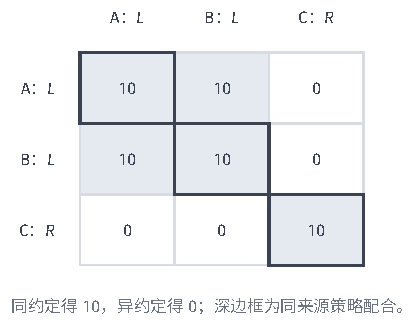
\includegraphics[width=69.977mm]{figures/10-reinforcement-learning/03-task-expansion-and-trustworthiness/tikz/rl-multi-agent-cross-play.pdf}
 \caption{两约定任务的交叉配合矩阵。各格给团队分，深边框标同来源对角；A、B使用$L$，C使用$R$，不兼容配对得0。数值由教学规则精确计算，并非实测成绩。}
 \label{fig:rl-multi-agent-cross-play}
\end{figure}

测试前应冻结训练群体、检查点选择和各伙伴的对局预算。可先对每个留出伙伴测零样本结果，再在预设$B\in\{0,5,20\}$等教学预算网格上测适应后表现；横轴记录实际交互，另列梯度步及记忆重置规则。若反复利用测试对手结果选检查点，它已被用于开发，需要重新留出，而非继续称为未见。

图中九格均匀平均为$50/9$，最差格为0，只平均三格对角却得到10。伙伴分布改变时，加权平均也改变，因此应同时报告矩阵、权重、平均和最坏已测表现。有限对局并未穷尽所有对手，最坏已测值仍不同于完整策略空间的最坏值，群体平均也不能提供不可利用性上界。

% Outline: 7.7.4
\subsection{固定样本、通信与计算预算下的效率评价}
\label{sec:rl-multi-agent-efficiency}

多智能体系统的资源消耗比单人复杂得多（一个联合环境步里其实包含$m$个参与者的动作），因此评价效率前必须统一计数口径，否则“更快”可能只是少算了某些通信或对手对局。

表\ref{tab:rl-multi-agent-resources}在每人$A$个离散动作、图边集$E_G$、消息维度$d_c$和消息传递轮数$L$的条件下，比较结构性操作成本。采样统一计联合步数$N$，达到某回报所需的$N$仍须实测。表中的计算阶数只说明列出的操作如何增长，不构成样本需求的推导。

\begin{table*}[htbp]
 \centering
 \begin{tabularx}{\linewidth}{@{}l >{\raggedright\arraybackslash}X >{\raggedright\arraybackslash}X >{\raggedright\arraybackslash}X >{\raggedright\arraybackslash}X@{}}
 \toprule
 结构 & 人数与动作计算 & 采样及训练权限 & 训练通信／存储 & 部署推理与通信\\
 \midrule
 联合价值枚举 & $m$人，$A^m$组合 & $N$联合步；集中输入 & 联合转移、动作与价值表或网络 & 若集中选动作，须具备实时集中权限\\
 VDN／QMIX & 局部比较$mA$次 & $N$联合步；QMIX混合器用状态 & 联合TD目标及训练反传 & $m$次局部网络；无必需执行消息\\
 集中评论家、局部行动者 & 每人一次动作输出 & $N$联合步；声明评论家状态／动作输入 & 回放或近期轨迹及集中特征 & 局部推理；共享参数不等于共享观测\\
 图消息策略 & $m$节点、$|E_G|$条边 & $N$联合步；合法训练图 & 消息及历史按实现记录 & $L|E_G|d_c$量级消息元素，$L$轮同步\\
 PSRO群体 & 双方各$K$个库策略 & 响应样本加收益表对局；权限继承响应器 & $K^2$表项及多个检查点 & 回合抽索引再执行；未必同时运行全部网络\\
 \bottomrule
 \end{tabularx}
 \caption{训练与部署的结构性资源需求。所列复杂度只针对对应操作，不等于总运行时间，也不证明达到某一回报的样本复杂度。}
 \label{tab:rl-multi-agent-resources}
\end{table*}

消息拓扑对成本的影响可由图\ref{fig:rl-multi-agent-scaling}的串行模型说明。设每条有向边处理一条消息耗时0.01毫秒，全部节点动作计算耗时$0.05m$毫秒。全连接具有$m(m-1)$条边；局部图在此按每人恰向$\min(4,m-1)$个出邻居发消息计算，共有$m\min(4,m-1)$条边，这是“最多4个”的满额情形。按节点和边逐项相加，得到
\[
 \begin{aligned}
 T_{\text{全连}}(m)&=0.05m+0.01m(m-1),\\
 T_{\text{局部}}(m)&=0.05m+0.01m\min(4,m-1).
 \end{aligned}
\]
代入$m=20$，两种解析时延分别为4.8和1.8毫秒。它们只成立于所给串行模型，并非硬件测试；真实设备的并行、拥塞及同步开销都可能改变结果。

\begin{figure}[htbp]
 \centering
 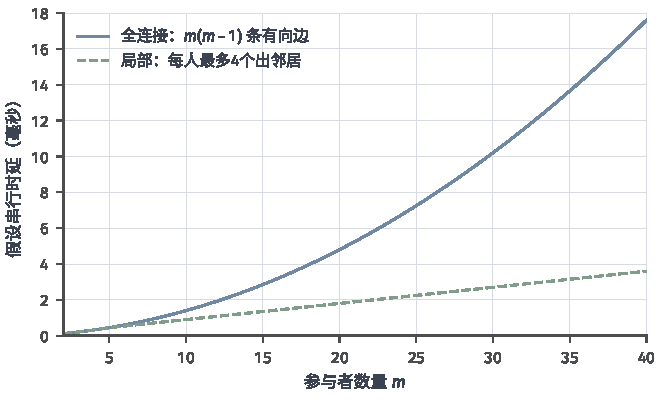
\includegraphics[width=112.000mm]{figures/10-reinforcement-learning/03-task-expansion-and-trustworthiness/matplotlib/rl-multi-agent-scaling.pdf}
 \caption{串行消息模型中的跨规模成本。全连接与最多4邻居的局部交互采用相同节点和边成本；稀疏图降低消息量，但可能同时删去任务需要的远端参与者状态或消息。}
 \label{fig:rl-multi-agent-scaling}
\end{figure}

资源比较应保留这些取舍：复用同一结构的参数可减少模型存储，却仍须为不同历史计算动作；集中状态与联合历史可帮助估计，却增加训练传输；通信可改善协调，却增加收发与同步开销，是否增加总时延还取决于并行实现。跨规模测试还须控制拥挤度、瓶颈容量和观测、历史与消息读取权限，否则成本增长与任务难度变化混在一起，难以解释曲线。

% Outline: 7.7.5
\subsection{行为评价与复现所需的协议信息}
\label{sec:rl-multi-agent-protocol}

多智能体结果尤其难复现，因为即使恢复了网络参数和随机种子，只要训练时的对手配对、各人行动前可读取的观测、历史与消息等交互条件没还原，结果就可能完全不同。因此复现不仅要恢复参数和随机种子，还须恢复参与者配对与交互权限。

\begin{table*}[htbp]
 \centering
 \small
 \begin{tabularx}{\linewidth}{@{}l >{\raggedright\arraybackslash}X >{\raggedright\arraybackslash}X@{}}
 \toprule
 协议项 & 必须记录的内容 & 主要影响环节\\
 \midrule
 参数共享与身份 & 共享哪些模块；编号、角色编码及重排规则 & 参数梯度汇总与执行约定\\
 集中状态与屏蔽 & 评论家输入；合法动作掩码由谁提供 & 训练权限及执行动作分布\\
 死亡、退出与终止 & 占位观测、动作、损失屏蔽；全局或个体终止 & 价值目标、占用统计和人数\\
 回放与版本 & 来源检查点、窗口、概率字段、校正与采样权重 & 联合经验的目标匹配\\
 对手与伙伴抽样 & 库版本、保留及淘汰、抽样概率、是否在线学习 & 训练和评价的参与者分布\\
 通信 & 发送／接收权限、载荷、时序、延迟、带宽 & 部署可行性与成本\\
 回报与评价 & 奖励尺度、塑形、回合上限、偏离类及间隙约定 & 行为标准和比较口径\\
 \bottomrule
 \end{tabularx}
 \caption{复现多智能体结果所需的最小协议。各项可能改变策略、环境或验证对象，因此超参数表之外还需保存这些交互条件。}
 \label{tab:rl-multi-agent-protocol}
\end{table*}

还应保存伙伴与对手的生成流程、策略库和检查点标识、用于检查点选择的验证参与者，以及各组合的评估场数。训练初始化、环境随机性和伙伴抽样宜采用可追踪的独立随机源。若5次独立训练各评价1000局，独立训练运行仍只有5个，不能把5000场对局当作5000次独立训练。同一检查点或同一适应链上的对局可能相关，区间估计应保留训练运行与伙伴层级。

第三方对手、外部游戏版本或消息服务若无法恢复，应列明限制。所存材料可以支持在这些伙伴与接口下重现结果，未必支持对所有未知参与者成立。只有声明、协议和证据对应同一对象，评价范围才清楚。

% Outline: 7.8
\section{本章小结}
\label{sec:rl-multi-agent-summary}

同一个通道动作会随对方行为产生不同后果，因而多智能体求解要先明确收益、观测与消息权限及参与者变化。收益关系决定采用团队最优、极小极大还是单方偏离标准，社会分配目标须另行规定；观测与消息读取权限限定策略可依赖的历史字段，集中训练不能扩大部署可见范围；其他人继续学习时，边缘化后的行为后果也可能不再平稳。

经验采集须记录联合动作、消息与参与者来源，并检查目标的联合支持；边缘动作都出现过，仍可能无法识别所需的配合效果。在此基础上，联合价值、个体替代、局部组合、伙伴类型和响应模型保留不同依赖，可共同提供更新所需的估计。价值或梯度计算还须与相互适应和群体组织配合。局部贪心一致不等于整表可表示，单次改进不等于共同动态稳定，库内近似响应也不能认证完整博弈不可利用。

验证时，外部与内部遗憾分别约束粗相关和相关经验分布；利用零和抵消才能进一步控制适当平均策略的鞍点间隙，当前策略却未必收敛。训练对手收益、留出伙伴协调、跨规模表现与资源成本也须分别报告。使用伙伴反馈更新记忆或类型已属适应，即使参数不变，也不能记为零样本。明确行为标准、参与者范围、可读观测与消息和交互预算之后，结果才有可解释的边界。第\ref{chap:rl-trustworthy}章将转向风险、扰动和安全约束这一类行为要求；性能证据并不自动成为安全保证，多方任务仍需保留本章的联合行为、局部观测与消息时序条件。

% Outline: 8
\chapter{可信强化学习}
\label{chap:rl-trustworthy}

前几章评价一个策略时，默认问题几乎只有一个：它的期望回报有多高。这个标准在多数回合表现正常时足够好用，却回答不了一类更尖锐的问题——“出状况的那几次怎么办”。考虑一台导航机器人：它在大多数回合很快到达终点，只在少数回合严重延误。平均到达时间即使很短，也把顺利回合和糟糕回合混在了一起，无法说明这些延误是否可以承受。更麻烦的是，训练时假设的环境与部署时未必相同：地面变湿时，原来学到的制动规律可能整体失效；而在机器人上启用一个会在危急时刻接管的紧急保护器后，“没有碰撞”又可能只是保护器替换了危险动作的结果，并不能说明原策略本身可靠。于是部署判断需要回答两个层次不同的问题：第一，我们究竟希望机器人满足什么行为要求——是平均表现好，还是最差的回合也不能太糟，是湿滑地面也要能用，还是任何时候都不许碰撞；第二，手头的证据——无论是有限的试验记录还是基于模型的证明——是否足以支持这些要求。前者是在规定“什么算合格”，后者是在核查“凭什么相信它合格”。

本章沿用第~\ref{chap:rl-overview}~章的策略与轨迹，以及第~\ref{chap:rl-planning}、\ref{chap:rl-learning}~章的规划和学习工具。回答第一个问题时，三种要求分别从三个不同的环节收紧决策：风险敏感决策改变的是随机后果的评价方式，例如不再只看平均损失，而比较最差那部分回合的损失；鲁棒决策改变的是环境范围，要求同一策略在允许的环境变化下都维持表现；安全约束改变的是可行策略集合，把不满足成本预算或边界要求的策略直接排除。三者改动的对象不同，可以组合使用，但并无必须依次采用的演进顺序。求出候选策略后，第二个问题——证据——才登场：此时评价一个已经冻结的策略、评价一条固定学习规则重复训练出的多个策略、以及评价一个带保护器的完整执行系统，是三种随机性来源不同、结论也不同的取证任务，必须分开处理。

图~\ref{fig:rl-trustworthy-map}~将三类要求放在相同的任务设定下。各分支先给出要维护的性质和求解方法，再由验证过程检查候选方案；方案比较中的保证只在相应运行条件和证据范围内成立。

\begin{figure*}[t]
  \centering
  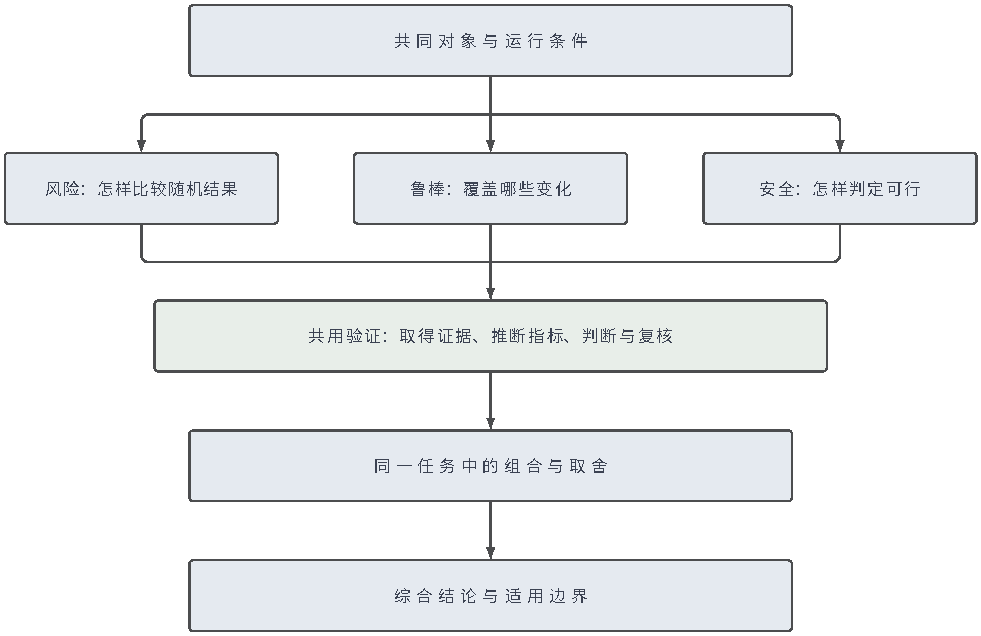
\includegraphics[width=166.169mm]{figures/10-reinforcement-learning/03-task-expansion-and-trustworthiness/tikz/rl-trustworthy-map.pdf}
  \caption{可信强化学习的章内关系。共同设定固定决策对象和运行条件，三个分支提出行为要求与候选策略，验证过程据此判断组合方案。箭头表示模型、策略、验证记录与结论之间的依赖，不表示风险、鲁棒与安全必须依次执行；综合结论仍保留各分支的适用条件。}
  \label{fig:rl-trustworthy-map}
\end{figure*}

% Outline: 8.1
\section{行为要求与保证对象}
\label{sec:rl-trustworthy-requirements}

要把上面三个要求讲清楚，先得学会做“只改一项条件”的受控比较——如果好几个因素同时变化，观察到的成功率改变就无法归因。仍考察从起点驶向终点的移动机器人。在相同的几何路线、初始位置与动力学下，比较不同速度控制策略诱导的到达时间分布，可以检查偶发严重延误；固定策略与目标，改变地面摩擦，可以检查制动距离。若环境不变，只把一块原本可以穿越的地带声明为危险区，改变的则是行为是否被允许的判定标准。最后，启用会替换危险动作的保护层，改变了实际执行机制。四种比较各自只改变一项条件，因而能够分别识别结果分布、环境变化、行为可行性和保护器的影响；一个总成功率无法区分这些影响。

离散导航示意沿用宽4、高3的网格、起点$(1,1)$、终点$(4,3)$和障碍$(2,2)$。数值例子会分别声明采用基准滑移模型，还是把整段路线汇总为一次选择的教学模型；路线模型用于手算，不是随机网格的精确解。连续控制仍写作$\bm{x}_{t+1}=\bm{A}\bm{x}_t+\bm{B}\bm{u}_t+\bm{w}_t$，状态可以包含位置和速度；允许扰动$\bm{w}_t$的范围来自另行给定的运行条件，不能从动力学方程本身读出。

在给出具体要求之前，先要统一描述“一次运行会产生什么、我们又能测量什么”，因为后面三类准则比较的正是这些不同的量。同一回合既可能效率高，也可能靠近过危险区，还可能发生碰撞；只用一个标量回报无法同时表达这些后果。下面先固定评价对象，再谈怎样用它们提要求。

\begin{definition}[回报、损失、成本与失败事件]
  \label{def:rl-trustworthy-objects}
  固定动态环境$\mathcal E$、观测与反馈机制和策略$\pi$，得到理论轨迹律$P_{\mathcal E}^\pi$；实际可取得的评价记录服从$P_{\mathrm{rec}}^\pi$。若损失含未记录状态，还须说明能否由这些记录识别损失的分布。记相应的轨迹样本空间为$\Omega_{\mathrm{traj}}$，其事件$\sigma$代数为$\mathcal F_{\mathrm{traj}}$（即我们能对其讨论“发生概率”的那些轨迹集合，例如“所有发生过碰撞的轨迹”构成的集合）。无限时域取$0\leq\gamma<1$，并要求下面的奖励和成本级数绝对可积；有界逐步奖励与成本足以满足这一条件。
  对轨迹$\tau=(s_0,a_0,r_0,s_1,\ldots)$，回报为
  $G(\tau)=\sum_{t\geq0}\gamma^t r_t$，目标$J(\pi)=\mathbb E_\pi G$不作归一化。
  损失$L(\tau)$表示需要抑制的后果，数值越大越差；它可以是累计延误，也可以是$-G$，但必须明确选择。
  安全成本$c_{i,t}\geq0$记录第$i$类危险暴露或损害，其累计量为
  $C_i(\tau)=\sum_{t\geq0}\gamma^t c_{i,t}$。
  失败事件$F_H\in\mathcal F_{\mathrm{traj}}$是轨迹空间中的可测事件，因而$F_H\subseteq\Omega_{\mathrm{traj}}$；例如，它可以表示前$H$次动作中至少碰撞一次。
  有限时域任务取正整数$H$，求和截至$H-1$，不折扣时直接使用有限和；其期望也要求相应累计量可积。
\end{definition}

导航任务中，奖励可以衡量到达效率，损失可以记录延误，成本可以累计靠近危险区的时间，失败事件可以定义为发生碰撞。优化方向也随对象而异：回报越大越好，损失和成本越小越好，事件概率则须低于给定阈值。同一次碰撞可以同时增加损失和成本，但成本能够区分事故次数或严重程度，事件指示量$\mathbf 1\{F_H\}$只记录是否发生；比较尾部损失还要问最差的一部分结果究竟有多严重。

有了这些量，就可以从三个互不替代的角度提要求。三者回答的问题分别是“随机结果怎样比较”“环境可以怎样变”“哪些行为根本不许做”。\term{风险准则}（risk criterion）规定怎样根据随机结果的分布比较策略，例如比较最差回合的延误，而非只比较均值。\term{鲁棒要求}（robustness requirement）规定同一策略必须应对哪些动力学、观测或动作执行机制的变化，例如摩擦的物理区间或传感器的误差范围。\term{安全约束}（safety constraint）规定哪些行为可行，例如成本不超过预算、碰撞概率低于阈值，或始终不离开允许状态集。这里的允许集合由任务规格、设备能力或模型误差界确定；算法负责在这些条件下求解，并不自行决定什么后果可以接受。

\term{可靠性}（reliability）在本章指指定对象在声明运行条件下持续满足要求的程度。这里需要特别区分“算法在优化什么”和“系统实际做到了什么”：算法采用了风险目标或安全约束，只说明它尝试优化什么，还没有说明交付对象实际满足什么。要把“可靠”从一个形容词变成可判断的结论，还需要统计或模型证据支撑。

同样说“这个策略可靠”，被评价的对象不同，结论的含义也完全不同，因此需要先锁定保证对象。表~\ref{tab:rl-trustworthy-guarantee-objects}~据此区分三种保证对象。策略冻结后，轨迹差异只来自环境与动作采样，重复运行相当于对同一随机机制重复抽样；重新训练时，还会加入训练记录的采集与回放次序、参数初始化和探索随机性的差异，两次训练可能得到两个不同的策略；保护层启用后，实际动作可能不同于策略提出的动作，碰撞记录所评价的便是策略与保护层的组合，而不是原策略本身。

\begin{table}[htbp]
  \centering
  \begin{tabularx}{\linewidth}{@{}>{\raggedright\arraybackslash}p{20mm}XXX@{}}
    \toprule
    保证对象 & 随机性来源 & 评价单位 & 要求作用时机 \\
    \midrule
    固定策略$\pi$ & 初态、转移、观测、动作采样 & 一个完整运行回合 & 策略冻结后的部署 \\
    学习规则 & 训练种子、训练样本、探索与优化 & 一次完整训练及其输出 & 训练中或输出策略上 \\
    策略与保护层 & 上述运行随机性，以及保护器所用状态估计、模型预测及动作执行的误差 & 实际执行系统的一回合 & 所有受保护执行时刻 \\
    \bottomrule
  \end{tabularx}
  \caption{保证对象决定抽样单位。每行还须固定初态分布、观测接口、时域、交互权限及其他参与者的范围，不能把训练曲线平稳等同于系统安全。}
  \label{tab:rl-trustworthy-guarantee-objects}
\end{table}

为了让“可靠”有可判定的含义，需要把运行范围写入协议：从哪些位置启动，摩擦允许怎样变化，传感器误差多大，能否主动试探，其他机器人按什么规则行动，以及保护器是否启用。后文的风险分布、鲁棒模型集合和安全可行集合都在这份协议下定义；改变协议，就可能改变原声明的真假。

协议还须区分两个极易混淆的百分数：行为概率与统计置信水平。前者描述系统本身多常出错，后者描述我们这套估计程序有多常给出正确结论。$p=\mathbb P_\pi(F_H)$表示策略在运行中多常失败；$1-\delta$表示反复采用取证与推断程序时，所得界覆盖真实$p$的比例要求。前者描述行为，后者描述推断程序。例如$p\leq0.01$是在限制失败概率，置信水平$0.95$是在限制程序的覆盖错误，两者不能交换。阈值、运行范围和允许的推断错误率须在验证前确定；根据结果反复修改标准，既改变行为声明，也可能破坏原有统计覆盖。

% Outline: 8.2
\section{风险敏感决策}
\label{sec:rl-trustworthy-risk}

从这一节起，先处理三个要求中的第一个：环境模型和运行范围都固定不变，只比较其中的随机后果。即便环境的概率规律完全已知且保持不变，策略的随机化、初态和转移的随机性也会让每一回合的损失不同；期望回报准则把这些差异平均掉，只保留一个数。当决策者真正在意的是糟糕回合时，就需要一套对分布形状敏感的评价方式。这里还有一个时间维度上的选择：决策者可以在出发前评价整段累计损失，并承诺执行据此选出的方案；也可以要求到达每个历史后，依据当前已取得的观测与损失记录，按同一种条件风险规则继续选择。前者评价出发时的结果分布，后者逐阶段评价条件分布。两者都可能通过递推求解，但递推形式相似不意味着目标相同——后面会看到，同一个方案在两种评价下甚至可能给出相反的选择。

% Outline: 8.2.1
\subsection{累计结果分布上的风险决策}
\label{sec:rl-trustworthy-static-risk}

为什么只看均值会漏掉关键的损失分布差别？用两个等均值分布最能说明问题。把到达时间抽象为无量纲损失，沿用两种等均值分布，以便随后检查策略随机化的尾部梯度：确定损失策略每回合损失恒为1，另一策略以0.95概率损失0、以0.05概率损失20。期望损失都是1，方差却分别为0和$0.05\times20^2-1^2=19$。均值相同，是因为多数回合的改善抵消了少数回合的严重损失；若最坏5\%的回合需要人工接管，决策者关心的恰是均值没有单独保留的这部分后果。可见期望这个汇总方式把顺利回合和糟糕回合直接相加，自动抹掉了分布形状上的差别；要识别这种差别，必须换一种打分方式。

第一种思路是改变“损失如何计分”：先把损失变换后再取期望，让大损失被额外放大。最小化$\mathbb E u(L)$时，若$u$在损失范围上递增且凸，增加同样大小的损失，在高损失处受到的惩罚不会更轻；凸性本身不保证惩罚严格增大，线性函数仍只按固定比例计分。对上述非负损失取$u(l)=l^2$，两个目标值分别为1和20，不过变换也改变了损失单位；允许负损失时，平方函数不再处处递增。

平方变换虽能区分两策略，但它仍对整个损失分布计分，没有直接选出“最差的那一小部分回合”。上述平方项衡量损失相对0的二阶偏离；在二阶矩有限时，把损失减去其均值后再平方取期望，得到的才是方差。也可以在均值上加入离散程度，得到\term{均值--方差准则}（mean--variance criterion）$\mathbb E L+\lambda\operatorname{Var}(L)$，其中$\lambda\geq0$调节惩罚强度。它需要二阶矩存在，且同时惩罚向均值两侧的偏离。若只想关注严重损失，分位数给出某个概率位置的阈值，尾部均值进一步汇总阈值之外的严重程度。这些准则分别使用损失的均值、方差、分位点或尾部平均，因而可能对同一组策略给出不同排序。要计算上尾，先按任务要求选定分位水平$\alpha$，例如$\alpha=0.95$对应最差5\%概率质量；损失越大越差，因此从高损失一侧选取。阈值可以在损失尺度上的实数中选择：分位点找累计概率至少达到$\alpha$的最低位置，尾部均值则用阈值加上缩放后的超额损失来表示，并对阈值取下确界。阈值的最小化只是在确定尾部计算方式，不是让决策者删去不利结果；下面的导数条件会说明它为何恰好选出所需概率质量。

固定概率空间上的实值可积轨迹损失$L$，即$\mathbb E|L|<\infty$；在策略评价中，该分布由已声明的环境、初态与策略诱导。连续、离散与混合分布统一使用左分位约定。对$0<\alpha<1$，\term{风险价值}（value at risk, VaR）与\term{条件风险价值}（conditional value at risk, CVaR）分别为
\begin{align}
 \operatorname{VaR}_\alpha(L)
 &=\inf\{z\in\mathbb R:\mathbb P(L\leq z)\geq\alpha\},\\
 \operatorname{CVaR}_\alpha(L)
 &=\inf_{\eta\in\mathbb R}\left\{\eta+\frac{\mathbb E(L-\eta)_+}{1-\alpha}\right\},
 \label{eq:rl-trustworthy-cvar}
\end{align}
其中$(x)_+=\max(x,0)$。前者给尾部阈值，后者平均最差$1-\alpha$概率质量，必要时只取分位点原子的一部分；这里用它们区分完整回合的随机后果，并构造后续尾部策略目标。分位、尾部与条件风险的一般分析可参考\BookChapterRef{chap:policy-value-and-optimization}{卷2《数学准备：概率、因果与决策》“策略的价值与优化”章}。

式~\eqref{eq:rl-trustworthy-cvar}~中的阈值只决定怎样选取尾部，不改变损失分布。令$F(z)=\mathbb P(L\leq z)$，阈值目标在$\eta$处达到最小值的条件为$F(\eta-)\leq\alpha\leq F(\eta)$。取左分位点$q_\alpha=\operatorname{VaR}_\alpha(L)$，相应尾部均值为
\begin{equation}
 \operatorname{CVaR}_\alpha(L)
 =\frac{\mathbb E[L\mathbf1\{L>q_\alpha\}]
       +q_\alpha\bigl((1-\alpha)-\mathbb P(L>q_\alpha)\bigr)}{1-\alpha}.
 \label{eq:rl-trustworthy-tail-mass}
\end{equation}
计算时先收入严格超过$q_\alpha$的全部损失，再从分位点原子补足尾部质量。直接取$\mathbb E[L\mid L\geq q_\alpha]$通常会纳入过多概率质量；离散回合损失的尾部估计必须检查这一差别。

代入两个教学分布，$\operatorname{VaR}_{0.95}$分别为1和0，$\operatorname{CVaR}_{0.95}$却分别为1和20。对第二个分布，若用$\mathbb E[L\mid L\geq0]$计算，会把全部样本纳入平均而得到1，不再是最差5\%的平均损失。图~\ref{fig:rl-trustworthy-loss}~因此画出离散概率质量：确定损失策略从1处原子只取5\%质量，另一策略则取20处全部5\%质量。均值重合并不妨碍分位点和尾部不同。

\begin{figure}[htbp]
  \centering
  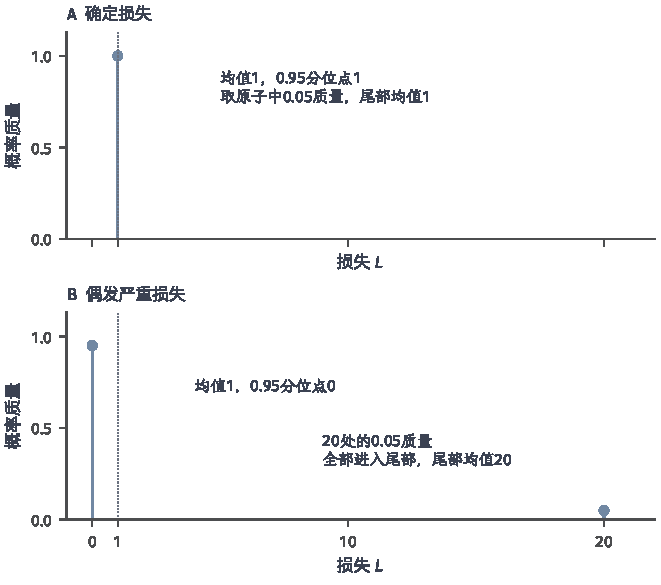
\includegraphics[width=112.000mm]{figures/10-reinforcement-learning/03-task-expansion-and-trustworthiness/matplotlib/rl-trustworthy-loss.pdf}
  \caption{两个教学损失分布，横轴为无量纲损失，纵轴为概率质量。粗实线和实心点表示原子，虚线标均值；图中文字说明用于计算CVaR的最差5\%质量，不是连续概率密度。}
  \label{fig:rl-trustworthy-loss}
\end{figure}

上面的定义假定损失分布已知。模型未知但允许运行当前策略时，可以直接用完整回合的样本估计累计损失，而不必先求转移核——因为我们只需要比较整个回合的后果，不需要知道每一步的转移核长什么样。设策略为$\pi_{\bm{\theta}}$，一回合损失为$L(\tau)$，把策略参数与尾部阈值组成联合目标
\[
  \Phi(\bm{\theta},\eta)
  =\eta+\frac{1}{1-\alpha}
      \mathbb E_{\tau\sim\pi_{\bm{\theta}}}(L(\tau)-\eta)_+.
\]
在环境不依赖策略参数、随机策略可微且支持不随参数突变，并能交换微分与期望的条件下，可用第~\ref{chap:rl-learning}~章的似然比方法求导。轨迹概率由逐步动作概率和环境转移概率相乘而成，环境项的参数导数为0，故其对数导数是
$\sum_{t=0}^{H-1}\nabla_{\bm{\theta}}\log\pi_{\bm{\theta}}(a_t\mid I_t)$。固定阈值，用超额损失加权这一轨迹得分，得到
\begin{equation}
  \nabla_{\bm{\theta}}\Phi
  =\frac{1}{1-\alpha}\mathbb E\left[
    (L-\eta)_+
    \sum_{t=0}^{H-1}\nabla_{\bm{\theta}}
       \log\pi_{\bm{\theta}}(a_t\mid I_t)\right].
  \label{eq:rl-trustworthy-tail-gradient}
\end{equation}
式~\eqref{eq:rl-trustworthy-tail-gradient}~中，未超过阈值的轨迹权重为0，超过阈值的轨迹按严重程度贡献策略更新。阈值本身的一个次梯度为
$1-(1-\alpha)^{-1}\mathbb P(L>\eta)$；在$L=\eta$处可以按$[0,1]$中的权重分配质量。算法~\ref{alg:rl-trustworthy-static-cvar}~据此同时更新阈值与策略，不需要把当前样本分位数当作真实分位数。

\begin{algorithm}[累计CVaR的轨迹更新]
  \label{alg:rl-trustworthy-static-cvar}
  \begin{algorithmic}[1]
    \Require 分位水平$\alpha$，时域$H$，批量$n$，步长序列，初值$\bm{\theta}^{(0)},\eta^{(0)}$
    \Ensure 候选策略及其阈值；可靠性另用留出评价样本验证
    \For{$k=0,\ldots,K-1$}
      \State 冻结当前参数，用$\pi_{\bm{\theta}^{(k)}}$独立启动$n$条轨迹，记录逐步损失并计算$L_j$
      \State 在旧参数、旧阈值上，用式~\eqref{eq:rl-trustworthy-tail-gradient}~的样本均值计算$\widehat{\bm{g}}_\theta$
      \State 计算$\widehat g_\eta=1-\frac{1}{n(1-\alpha)}\sum_j\mathbf 1\{L_j>\eta^{(k)}\}$，按需处理阈值处原子
      \State $\bm{\theta}^{(k+1)}=\bm{\theta}^{(k)}-\alpha_{\theta,k}\widehat{\bm{g}}_\theta$，
        $\eta^{(k+1)}=\eta^{(k)}-\zeta_k\widehat g_\eta$
    \EndFor
  \end{algorithmic}
\end{algorithm}

回到两条路线，可以直接检查梯度的行为含义。设出发时以概率$p=\operatorname{sigmoid}(\theta)$选偶发严重损失策略，否则选确定损失策略。对$0\leq p\leq1$，最差5\%质量由$0.05p$的损失20和$0.05(1-p)$的损失1组成，CVaR为$1+19p$。在$p=1/2$、最优阈值$\eta=1$处，精确策略梯度为$19p(1-p)=4.75$；沿负梯度更新会减小$\theta$，进而减少选择高尾部损失路线的概率。这个数由分布解析计算得到，不是训练实验的结果。

每批需要$nH$次交互与相应的策略求导，保存整批轨迹的空间也与$nH$成正比。经验分位数若通过排序求得，另需$O(n\log n)$；阈值次梯度只需$O(n)$。尾部估计还受有效回合数限制：用于最差部分的样本量约为$n(1-\alpha)$，这个数很小时，更新依赖极少数尾部回合，一整批也可能没有关键严重事件。误差还取决于损失尾部的大小及矩条件，不能只由这一回合数判断。

同批完整轨迹若既用于选择策略，又用于报告其尾部损失，还会引入选择偏差。模型轨迹能够减少真实交互，但模型在罕见区域的误差会直接影响尾部目标。百分位风险约束中的策略梯度和行动者--评论家方法同样需要估计风险、更新策略并调整约束，其局部收敛结论依赖特定假设；这些结论既不消除尾部估计误差，也不是任意神经网络训练的全局最优保证\scite{rl8-chow2018-percentile}

与无模型方法相对，已知有限时域模型时，也可以用动态规划求同一个静态目标，关键在于补齐状态。以累计损失
$L=\sum_{t=0}^{H-1}\gamma^t\ell_t$为例，只保存物理状态无法知道终点的超额损失，因而再记录已经积累的损失$z$。先固定出发前选定的$\eta$，把终端目标设为$(z-\eta)_+$，再用普通期望向后递推：
\begin{align}
  W_H^\eta(s,z)&=(z-\eta)_+, \nonumber\\
  W_t^\eta(s,z)&=\min_{a\in\mathsf A(s)}
       \mathbb E\!\left[
       W_{t+1}^\eta(s',z+\gamma^t\ell_t)\mid s,a\right].
  \label{eq:rl-trustworthy-augmented-risk}
\end{align}
再在出发前最小化
$\eta+(1-\alpha)^{-1}\mathbb E_{s_0\sim\mu_0}W_0^\eta(s_0,0)$。
每步把$\gamma^t\ell_t$加到累计量中，模型期望同时覆盖后继状态与本步损失；策略因此可以依赖时间、状态和已观察的累计损失。损失支持离散且有限时，可枚举可达$z$；$z$连续时，离散化或插值会扩大状态规模并引入误差。阈值仍属于事前承诺，途中重置为新的条件分位数会改变目标。另有增广方法保存尾部概率预算；原论文以尾部质量为参数，换成本章记号时应使用$1-\alpha$\scite{rl8-chow2015-cvar}

\begin{example}[静态CVaR的时间不一致]
  \label{ex:rl-trustworthy-time-inconsistency}
  设$H=2$且不折扣。$t=0$只有一个虚拟动作，损失为0，随后进入可观察的分支A或B，概率分别为0.1与0.9。$t=1$在B只有一个动作，损失固定为10；在A可以选safe，损失12，也可以选risky，损失以0.9概率为0、以0.1概率为20。决策者在$t=0$选择并承诺一个完整条件策略，在到达A后执行约定动作。

  取$\alpha=0.9$。承诺safe时，总损失分布为$10(0.9),12(0.1)$，CVaR为12。承诺risky时，分布为$0(0.09),10(0.9),20(0.01)$，最坏10\%由全部1\%的20和9\%的10组成，所以
  \[
    \operatorname{CVaR}_{0.9}(L_{\text{risky}})
       =\frac{0.01\times20+0.09\times10}{0.1}=11.
  \]
  事前准则严格选择risky。但一旦到达A，重新最小化条件CVaR，safe与risky的数值分别为12与20，因而严格选择safe。环境和可选动作没有改变，改变的是条件化之后用于定义尾部的概率质量。
\end{example}

反例中分支已被观察，冲突仍然发生：到达A后，定义最差10\%时不再计入B的概率质量。静态CVaR若只在原物理状态上套用普通Bellman递推，就可能丢掉事前评价的这层含义。式~\eqref{eq:rl-trustworthy-augmented-risk}~通过累计损失和固定阈值保留事前目标；若任务反而要求每个历史下都按当前条件重新评价，则需要下一小节的动态目标。

% Outline: 8.2.2
\subsection{逐阶段条件风险下的决策}
\label{sec:rl-trustworthy-dynamic-risk}

静态准则的时间不一致反例提示了另一种决策观：如果决策者不打算事先承诺，而是保留在每次取得新的观测、奖励或损失记录后重新决策的权利，就需要逐阶段地评价风险。到达A后，B已经被排除，未来方案可以只按A下的后果比较。\term{条件风险映射}（conditional risk mapping）执行的就是这一步：把下一阶段的不确定损失汇总成以当前已揭示记录为条件的风险数值。该数值在当前历史下已知，在更早时刻却仍可能随机。令$\mathcal F_t$为截至时刻$t$已揭示的状态或观测、已执行动作及已到达奖励或损失记录生成的$\sigma$代数；协议额外给出的公共信号也一并纳入。映射$\rho_t$把$\mathcal F_{t+1}$可测损失变成$\mathcal F_t$可测量。条件CVaR在式~\eqref{eq:rl-trustworthy-cvar}~中改用$\mathbb E[\cdot\mid\mathcal F_t]$，阈值也改为$\mathcal F_t$可测的随机变量；一般概率空间上使用本质下确界，即忽略零概率集合后仍成立的最大下界。有限树上，这等于在每个正概率历史的条件分布内分别优化阈值。不同策略的风险各自按其诱导分布计算；要比较这种排序能否跨时刻保持，则须在同一概率空间及同一组按时刻递增的$\sigma$代数下进行，不将不同策略的两条轨迹直接逐点配对。这样的几乎处处结论也不自动覆盖运行分布未支持的历史。

为将条件风险用于逐阶段交互控制，固定正整数时域$H$、$0\leq\gamma\leq1$、概率空间$(\Omega,\mathcal F,\mathbb P)$及递增$\sigma$代数族$\mathcal F_0\subseteq\cdots\subseteq\mathcal F_H$。令$L^\infty(\mathcal F_t)$表示相对于$\mathbb P$几乎处处有界、在$\mathcal F_t$下可测的随机变量。
  取归一化$\rho_t(0)=0$的一步条件风险映射$\rho_t:L^\infty(\mathcal F_{t+1})\to L^\infty(\mathcal F_t)$。对阶段损失$\ell_t\in L^\infty(\mathcal F_{t+1})$，定义
  \[
    \mathcal R_t
      =\rho_t(\ell_t+\gamma\mathcal R_{t+1}),
      \qquad \mathcal R_H=0.
  \]
  这一递归是\term{嵌套风险}（nested risk），即把后一步风险当作当前待评价的未来损失。
  动态风险族具有\term{时间一致性}（time consistency），如果对任意$0\leq u<v\leq H$和上述同一空间上的两个损失序列，它们在$u,\ldots,v-1$几乎处处相同，且$v$时刻的条件风险几乎处处满足$\mathcal R_v\leq\widetilde{\mathcal R}_v$，就有
  $\mathcal R_u\leq\widetilde{\mathcal R}_u$。
  所有几乎处处比较均相对于同一个$\mathbb P$。有界空间使逐层输入和输出仍在映射定义域内；无界损失的动态风险须另给可积性与定义域封闭条件，不能只沿用静态CVaR的可积假设。

共同概率空间可以先按一棵固定的随机树理解：分支、分支概率和前段损失不变，只比较两套后续损失。例如两个叶节点上的损失分别为$X=(2,4)$与$Y=(3,5)$，就能在同一叶节点逐项比较$X\leq Y$；单调的条件风险把这种排序逐层向前传递。这里检查的是同一条件风险规则怎样评价不同损失，并不是把两个机器人各自运行得到的轨迹强行配对。

控制优化还要加入动作对后继分布的影响。不同动作可以产生不同的下一状态分布，因而下面分别用$\rho_{t,s,a}$表示给定状态动作后的一步条件风险。先按每个动作对应的条件分布计算风险，再比较动作，与前面的共同空间排序性质并不冲突。

时间一致性保留跨时刻的排序：两方案前段损失相同，若以后在每个可能历史下一个方案的条件风险都不更高，较早评价也不应把它排得更差。各$\rho_t$单调时，将$v$时刻的不等式逐层代入递归，就能传到$u$。这一论证控制的是条件风险排序，并未断言每条轨迹都没有损失。动态风险及其Markov表示的系统论述见原始工作\scite{rl8-ruszczynski2010-risk}

在示例~\ref{ex:rl-trustworthy-time-inconsistency}~中，每层采用$\alpha=0.9$的条件CVaR。先在A内汇总叶节点，risky得到20，safe得到12；B的风险为10。再汇总分支风险$20(0.1),10(0.9)$，risky的嵌套风险为20，safe则为12。图~\ref{fig:rl-trustworthy-risk-tree}~对照这两种运算：静态准则直接使用叶节点的联合概率，嵌套准则先把分支后果压成条件风险。选择从risky变为safe，来自评价对象改变，而非静态求解精度提高。

\begin{figure*}[t]
  \centering
  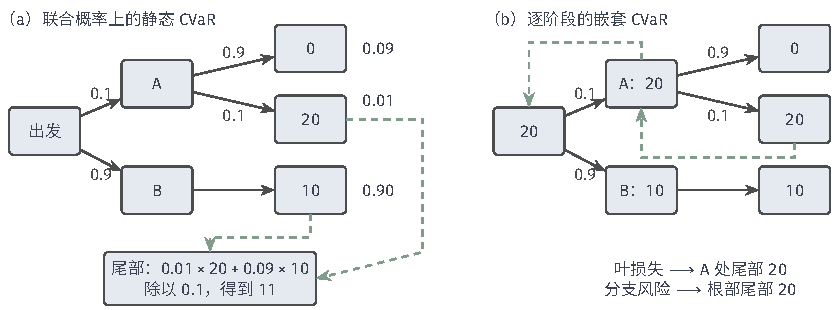
\includegraphics[width=141.390mm]{figures/10-reinforcement-learning/03-task-expansion-and-trustworthiness/tikz/rl-trustworthy-risk-tree.pdf}
  \caption{同一教学决策树的两种风险汇总，均取$\alpha=0.9$、$H=2$且不折扣。图中展示承诺risky的分支；实线表示随机转移，带文字的回传箭头表示风险计算。safe只需将A的两个叶节点替换为固定损失12。}
  \label{fig:rl-trustworthy-risk-tree}
\end{figure*}

分支树可以逐层回传，状态价值递推却还要求状态保存决定后继条件分布和风险映射的历史记录、累计损失或剩余预算。这里要求给定$(t,s,a)$后，后继条件分布、风险映射及其水平不再依赖未记录的历史；各映射在相应条件分布的有界后继变量上定义，并满足单调性，使后续风险的改善能够传到当前评价。设动作确定后，一步损失$\ell(s,a)$已知，$\rho_{s,a}$只评价后继状态上的随机量。若风险满足平移等变性，即加上当前已知常数会使风险增加同一常数，就能把这一步损失移到映射外。有限时域Markov风险问题于是可向后归纳为
\begin{equation}
  V_t(s)=\min_{a\in\mathsf A(s)}
    \{\ell_t(s,a)+\rho_{t,s,a}(\gamma V_{t+1}(s'))\},
  \qquad V_H=0.
  \label{eq:rl-trustworthy-risk-bellman}
\end{equation}
式~\eqref{eq:rl-trustworthy-risk-bellman}~先评价每个动作下的未来风险，再选损失风险最小的动作。一步损失若也随机，须将$\ell_t+\gamma V_{t+1}$一起放入联合分布的风险映射；风险水平若依赖剩余预算或历史，相应的剩余预算或历史记录也须进入状态。这里采用确定性Markov动作选择。允许随机动作时，还要规定风险在随机化之前还是之后评价，否则算子所优化的目标并未确定。

\begin{theorem}[折扣风险算子的压缩性]
  \label{thm:rl-trustworthy-risk-contraction}
  设状态集$S$及每个可行动作集$\mathsf A(s)$有限且非空，确定阶段损失$\ell(s,a)$有界，$0<\gamma<1$。对每个$(s,a)$，固定后继条件分布及风险规则，映射$\rho_{s,a}:\mathbb R^{|S|}\to\mathbb R$在所有有限后继值向量上有定义，迭代中不改变；所需历史已计入状态。
  每个映射满足单调性，即逐后继状态$X\leq Y$推出$\rho_{s,a}(X)\leq\rho_{s,a}(Y)$，并对任意实常数$b$满足平移等变性
  $\rho_{s,a}(X+b)=\rho_{s,a}(X)+b$。
  对已经按声明的风险问题建立的算子
  \[
    (\mathcal B V)(s)=\min_{a\in\mathsf A(s)}\{\ell(s,a)+\rho_{s,a}(\gamma V(s'))\},
  \]
  对任意$V,W\in\mathbb R^{|S|}$，有$\lVert\mathcal B V-\mathcal B W\rVert_\infty\leq\gamma\lVert V-W\rVert_\infty$。
  因而该算子有唯一不动点，反复应用$\mathcal B$从任意有限初值收敛到该点。
\end{theorem}
\begin{proof}
  令$\varepsilon=\lVert V-W\rVert_\infty$。对所有后继状态，
  $\gamma W-\gamma\varepsilon\leq\gamma V\leq\gamma W+\gamma\varepsilon$。
  单调性把不等式传入$\rho_{s,a}$，平移等变性把两端的常数移出，得到
  \[
    \rho_{s,a}(\gamma W)-\gamma\varepsilon
      \leq\rho_{s,a}(\gamma V)
      \leq\rho_{s,a}(\gamma W)+\gamma\varepsilon.
  \]
  记每个动作的花括号表达式为$q_V(s,a)$和$q_W(s,a)$，则
  $|q_V-q_W|\leq\gamma\varepsilon$。对所有动作的下界取最小值，得
  $(\mathcal B V)(s)\geq(\mathcal B W)(s)-\gamma\varepsilon$；取上界的最小值，得反向界。因此所需无穷范数界成立。

  $\mathbb R^{|S|}$配无穷范数是非空完备度量空间，上述算子把它映回自身，且压缩因子为$\gamma<1$。压缩不动点结论因此给出唯一不动点及任意有限初值的几何收敛，并有
  $\lVert V^{(k)}-V^\star\rVert_\infty\leq\gamma^k\lVert V^{(0)}-V^\star\rVert_\infty$。
  相关基础可参考\BookChapterRef{chap:metric-spaces}{卷1《数学准备：计算、分析与几何》“度量空间”章}。这里保证的是已经按声明风险建立的固定算子的求解，不保证环境或风险模型本身正确。
\end{proof}

证明用单调性传递上下界，用平移等变性移出误差常数，没有使用正齐次性，因而将折扣留在$\rho(\gamma V)$内部即可。它回答的是价值迭代是否收敛。不动点是否代表希望求解的风险目标，还须核对时间一致性、状态所保存的历史与预算和允许策略类，数值压缩性本身不证明这些建模条件。

以已知有限模型的条件CVaR价值迭代为例，每轮先冻结$V^{(k)}$。对每个$(s,a)$，列出后继值$\gamma V^{(k)}(s')$及概率，按值排序并从最大值累计$1-\alpha$质量，再由式~\eqref{eq:rl-trustworthy-tail-mass}~求风险；加上$\ell(s,a)$后，对动作取最小值。排序是在寻找严重损失尾部，动作最小化则是在改善决策。迭代到残差
$\lVert\mathcal B V^{(k)}-V^{(k)}\rVert_\infty\leq(1-\gamma)\epsilon$时，
压缩界与三角不等式给出
$\lVert V^{(k)}-V^\star\rVert_\infty\leq\epsilon$。
在两阶段树上，从终端0开始，A的回传立即得到$\min(12,20)=12$，B得到10，根部再得到12，完成一次可复核的向后计算。

记状态数为$m$、每状态最多$b$个动作，稠密转移下每轮排序更新需$O(bm^2\log m)$，模型存储需$O(bm^2)$。若只有指定状态动作的采样接口，就需用独立后继批次估计条件分布；条件CVaR是分布的非线性函数，单个后继样本的风险一般不能无偏估计总体风险。每步近似算子误差若一致不超过$e$，迭代误差满足
$\Delta_{k+1}\leq\gamma\Delta_k+e$，长期误差上限为$e/(1-\gamma)$。
因此，风险策略梯度需要与嵌套目标相符的风险权重，分布评论家则需估计相应的条件后果分布。把期望评论家的价值预测换成尾部分位数，只改变了一个预测量；还须推导它如何参与目标和更新，才能得到所声明的风险算法。

% Outline: 8.3
\section{不确定环境下的鲁棒决策}
\label{sec:rl-trustworthy-robust}

风险准则处理的是一个固定概率模型内部的随机性。现在放宽“模型已知且准确”这个前提：部署环境可能与训练时不同，问题转为同一策略能否在允许的变化范围内维持要求。注意这里不假设各环境以某个概率出现——工程师通常只知道摩擦的物理区间、传感器的误差规格，而不知道“今天是干地还是湿地”的概率，因此不能简单取期望，只能保证整个范围内的最坏表现。变化进入系统的位置不同，应对手段也不同。图~\ref{fig:rl-trustworthy-channels}~固定交互闭环，区分三个扰动位置：摩擦变化影响真实状态转移，传感读数修改影响策略读取的观测，制动力削弱影响请求动作的实际执行。对抗训练是在这些位置搜索不利变化的求解手段，不是第四种扰动对象。

\begin{figure*}[t]
  \centering
  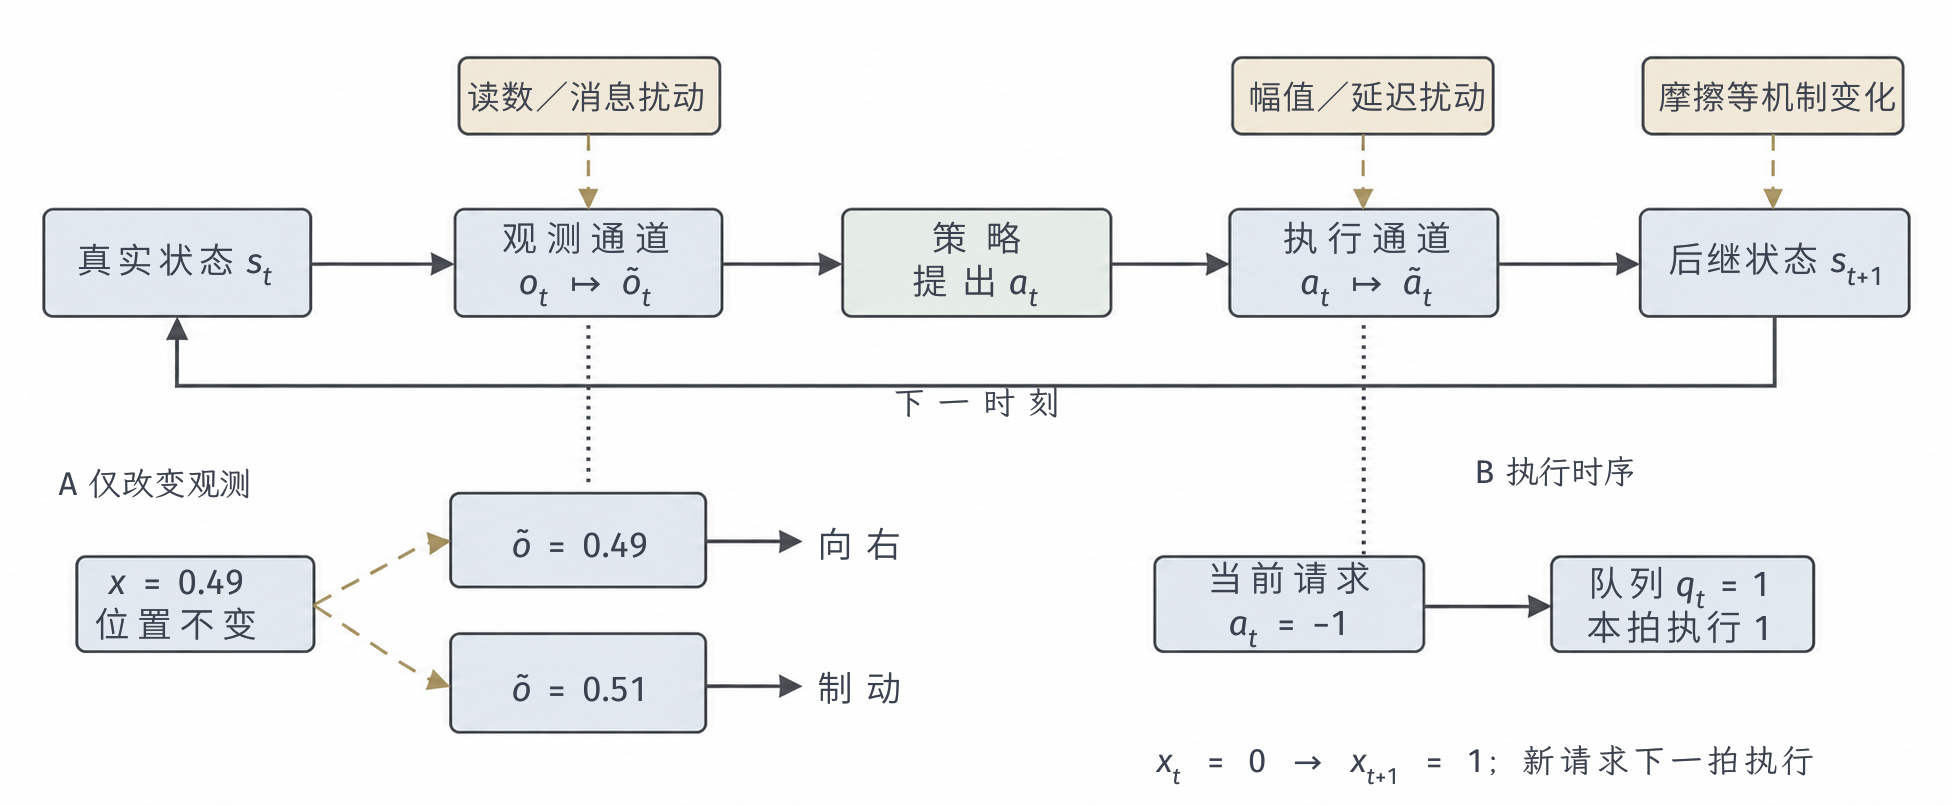
\includegraphics[width=157.400mm]{figures/10-reinforcement-learning/03-task-expansion-and-trustworthiness/generated/rl-trustworthy-channels/figure.png}
  \caption{扰动进入交互闭环的三个位置。实线传递状态、观测与动作，虚线表示不同扰动权限。下方两个局部面板分别只突出观测误差和执行延迟，二者均不等于直接改变当前真实位置。点状引线只定位下方对应通道的局部示意，不表示额外运行路径。}
  \label{fig:rl-trustworthy-channels}
\end{figure*}

% Outline: 8.3.1
\subsection{环境机制变化下的鲁棒决策}
\label{sec:rl-trustworthy-mechanism}

先处理动力学本身的不确定性。摩擦系数的点估计0.6给出标称模型$\widehat T$，用它规划相当于赌真实摩擦恰好是0.6；物理测量若只支持区间$[0.4,0.8]$，则给出一族可能转移核$\mathcal U$，鲁棒规划要在这一族上都站得住。前者适合预测标称表现，后者适合检查整个允许范围内的不利表现。固定奖励$R$和初态分布$\mu_0$，只让转移核变化，从而单独识别动力学不确定性的影响。区间没有规定各模型出现的概率，因而尚不能对模型作概率平均；即使另给概率权重，平均回报较高也可能掩盖某个允许模型下的低回报。要为集合内每个模型提供统一下界，就先对同一策略取回报的下确界，再选择这个下界最大的策略；每个模型内部的随机轨迹仍由$J_T(\pi)$取期望。

\begin{definition}[最坏情形回报]
  \label{def:rl-trustworthy-robust-return}
  固定有限状态动作、非空可行动作、有界奖励$R$、初态分布$\mu_0$和$0\leq\gamma<1$。令$\mathcal U$为非空允许转移核集合，各核均给出每个状态动作下的概率分布；$J_T(\pi)$是在核$T$下由$\mu_0$启动、按策略$\pi$运行的期望折扣回报。给定非空合法候选策略类$\Pi$，其中每条策略均按其获准历史选择合法动作。对固定$\pi\in\Pi$，鲁棒回报及该类中的最优值为
  \[
    J_{\mathrm{rob}}(\pi)=\inf_{T\in\mathcal U}J_T(\pi),
    \qquad J_{\mathrm{rob}}^\star=\sup_{\pi\in\Pi}J_{\mathrm{rob}}(\pi).
  \]
  集合$\mathcal U$描述允许的环境，而不是轨迹中随机转移结果的集合。若奖励或初态也不确定，应把它们与$T$一起列入模型集合。
  候选类$\Pi$还须指定允许确定性、随机化和历史依赖的范围。最优值能否由某条策略取到需另证；保证取到以后，才可把上确界写成最大值。
\end{definition}

区间可以来自设备的物理界，也可以来自转移记录的联合置信区域；两种来源的保证不同。若$\mathcal U=\mathcal U(D)$由转移记录$D$构造，模型假设还需附带统计覆盖事件
$\{T_{\text{真}}\in\mathcal U(D)\}$。在该事件上，任何被评价策略都有
$J_{T_{\text{真}}}(\pi)\geq\inf_{T\in\mathcal U}J_T(\pi)$。
这是集合内的确定性比较：真实模型只要被包含，最坏回报便是其回报下界。集合若以至少$1-\delta$的概率覆盖真实模型，才能进一步形成带置信水平的声明。集合过小可能漏掉真实环境，过大则可能降低可保证的回报，付出不必要的保守代价。鲁棒MDP需要同时说明集合结构和转移记录所给出的置信区域\scite{rl8-wiesemann2013-robust}

最坏回报定义是对整个模型一次性取最坏，但Bellman备份每次只处理一个状态动作；要让局部选择拼出一个合法的全局最坏环境，集合还须能够分解。\term{状态--动作矩形性}（state-action rectangularity）指
$\mathcal U=\prod_{s,a}\mathcal U_{s,a}$，也就是从各局部集合任选一个转移分布，组合后仍是允许模型。相应动态对手看到当前状态和已选动作后，在$\mathcal U_{s,a}$中选择下一步分布，不受跨状态或跨时间的共享剩余预算约束。下面采用最小值写法时，还要求各$\mathcal U_{s,a}$是概率单纯形中的非空紧集，使连续的线性目标能够取到最小值；若只知道局部集合非空而不能保证取到，则应把内层写成下确界。按这些条件与权限得到
\begin{equation}
  (\mathcal B_{\mathrm{rob}}V)(s)
    =\max_{a\in\mathsf A(s)}
      \left\{R(s,a)+\gamma
        \min_{p\in\mathcal U_{s,a}}\sum_{s'}p(s')V(s')\right\}.
  \label{eq:rl-trustworthy-robust-bellman}
\end{equation}
式~\eqref{eq:rl-trustworthy-robust-bellman}~的外层最大化回报，内层最小化给定动作下的后继价值。先选动作再让对手选择分布，正是前述对手读取当前状态与动作的权限；若对手须在看到动作前承诺一个跨动作共享的参数，允许的局部选择会变少，不能直接沿用同一算子。

\begin{theorem}[矩形鲁棒Bellman算子的压缩性]
  \label{thm:rl-trustworthy-robust-contraction}
  设状态集$S$及可行动作集$\mathsf A(s)$有限且非空，奖励$R(s,a)$有界，$0<\gamma<1$，每个$\mathcal U_{s,a}$都是$S$上概率单纯形中的非空紧集。令全局转移核集合为$\mathcal U=\prod_{s,a}\mathcal U_{s,a}$，对手在当前状态和动作已知后选择本步分布，不受跨步共享约束；状态是双方所用历史的共同充分表示。固定这些奖励、集合与权限后，式~\eqref{eq:rl-trustworthy-robust-bellman}~作为$\mathbb R^{|S|}$上的算子，在无穷范数下是$\gamma$压缩映射。
\end{theorem}
\begin{proof}
  令$\varepsilon=\lVert V-W\rVert_\infty$。对任意概率向量$p$，
  \[
    \left|\sum_{s'}p(s')V(s')-\sum_{s'}p(s')W(s')\right|
      \leq\sum_{s'}p(s')\varepsilon=\varepsilon.
  \]
  记内层最小值为$m_V,m_W$。上式对集合中每个$p$都成立，故
  $\sum pV\geq\sum pW-\varepsilon\geq m_W-\varepsilon$，取最小值得
  $m_V\geq m_W-\varepsilon$。由于紧性保证$W$的最小点$p_W$存在，
  $m_V\leq\sum p_WV\leq m_W+\varepsilon$。于是$|m_V-m_W|\leq\varepsilon$。
  加入相同的$R(s,a)$并乘以$\gamma$，每个动作的表达式相差至多$\gamma\varepsilon$。
  对各动作的上下界分别取最大值，得到
  \[
    (\mathcal B_{\mathrm{rob}}W)(s)-\gamma\varepsilon
      \leq(\mathcal B_{\mathrm{rob}}V)(s)
      \leq(\mathcal B_{\mathrm{rob}}W)(s)+\gamma\varepsilon.
  \]
  对状态取最大绝对差，结论成立。不动点存在、唯一及价值迭代收敛，由定理~\ref{thm:rl-trustworthy-risk-contraction}~中使用的非空完备空间上的压缩不动点结论得到。
\end{proof}

压缩证明控制的是数值迭代，矩形性则把局部最坏选择接成合法的全局环境。不动点处，各状态可取一个外层最优动作，各状态动作可取一个内层最差分布；由于这些分布可自由组合，它们共同给出$T^\star\in\mathcal U$。固定平稳Markov策略时，将外层最大化换成按$\pi(a\mid s)$平均，保留各动作下的内层最小化，就得到该策略在矩形模型族中的最坏回报评价。

历史依赖策略还需在状态中保留所用记忆，但状态增广不自动产生矩形性。若以$(s,m)$表示物理状态与记忆，同一个物理参数在不同记忆副本间共享的关系仍须保留；不能仅因$m$不同，就允许对手分别选择彼此不相容的参数。否则得到的是更大的不确定集合，后面的共享参数示例~\ref{ex:rl-trustworthy-coupling}~说明了这种扩大怎样改变最坏回报。局部备份与动态对手的对应，由有限时域逐步归纳和无限时域折扣极限建立；有限时域模型族还须允许各时刻局部分布独立组合。空间上的矩形性并不自动赋予时间上的自由变化，任意耦合集合也不满足这套分解条件。

求解式~\eqref{eq:rl-trustworthy-robust-bellman}~时，置信多面体使内层成为线性目标$\sum pV$的线性规划；只有两个后继状态的概率区间时，线性目标在端点取最小值。教学例取后继价值10与0、$\gamma=0.9$、当前奖励0，好状态概率$p\in[0.7,0.9]$。最坏选择为$p=0.7$，备份为$0.9\times0.7\times10=6.3$；标称$p=0.8$时为7.2。另一动作若确定到达价值7.5的后继，其备份为6.75，于是标称选择第一个动作，鲁棒选择第二个动作。

每轮冻结旧价值，逐状态动作求内层最小值，再取外层最大值。记一次内层优化代价为$C_{\text{内}}$，每轮需$O(mbC_{\text{内}})$。内层求解残差、模型集合估计误差和价值逼近误差影响不同步骤，应分别记录，不能只报告最终迭代残差。

\begin{example}[共享参数不能随状态独立取坏值]
  \label{ex:rl-trustworthy-coupling}
  一个两阶段教学任务以相同概率从$s_1,s_2$启动，各只有一个动作，第一步奖励0。下一步到达成功状态得到奖励1，失败状态得到0，随后终止。整个环境共享一个固定未知参数$\vartheta\in[0,1]$，成功概率分别是
  $p_1=\vartheta$与$p_2=1-\vartheta$。
  对任意合法环境，初态平均回报都为
  $\gamma(p_1+p_2)/2=\gamma/2$。
  如果只保留每个概率各自属于$[0,1]$，逐状态最坏选择会取$p_1=p_2=0$，得到回报0；然而不存在同时产生这两个概率的$\vartheta$。
\end{example}

图~\ref{fig:rl-trustworthy-rectangular}~的斜线给出共享参数真正允许的组合，方形则允许局部概率各自取坏值。扩大集合的算子即使严格收敛，也是在解更保守的另一个问题。共享参数若能由历史观测逐渐识别，新观测还可能通过辨识共享参数来改善后续控制；保留参数信念或相关历史才能利用它，将每次访问都当作对手重新任意选参数会丢掉这一机会。

\begin{figure}[htbp]
  \centering
  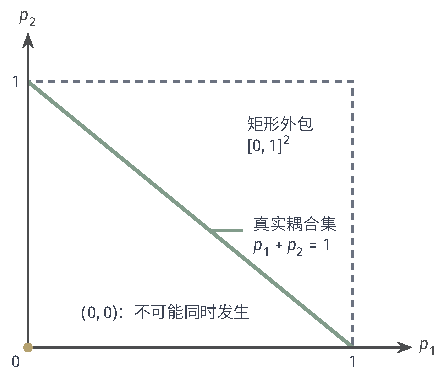
\includegraphics[width=75.805mm]{figures/10-reinforcement-learning/03-task-expansion-and-trustworthiness/tikz/rl-trustworthy-rectangular.pdf}
  \caption{教学耦合集$\{(p_1,p_2):p_1+p_2=1\}$与矩形外包$[0,1]^2$。方形左下角给出局部最坏选择，却不属于共享参数模型。坐标是两状态的成功概率。}
  \label{fig:rl-trustworthy-rectangular}
\end{figure}

“分布鲁棒”仍须说明哪个分布不确定。可能变化的是后继状态转移分布$p(\cdot\mid s,a)$，也可能是随机环境参数$\vartheta$的分布$\nu$；后一种问题优化
$\inf_{\nu\in\mathfrak U}\mathbb E_{\vartheta\sim\nu}J_{T_\vartheta}(\pi)$。
回合开始时抽取模型并保持不变，会使整段轨迹共享参数；每步重新抽取通常产生不同过程。Xu与Mannor的分布鲁棒MDP用参数分布的嵌套集合约束表示已知的参数概率或概率界，并建立相应状态分解与求解条件；这些条件不是把任意参数分布歧义集逐状态拆开的许可\scite{rl8-xu2010-distributional}

表~\ref{tab:rl-trustworthy-uncertainty}~按不确定对象对齐集合来源和求解条件。其他参与者造成的转移变化，还须符合第~\ref{chap:rl-multi-agent}~章的联合行为模型，不能擅自赋予其任意局部变化权限；识别未知参数后再适应，则涉及第~\ref{chap:rl-transfer}~章的任务推断。

\begin{table}[htbp]
  \centering
  \begin{tabularx}{\linewidth}{@{}>{\raggedright\arraybackslash}p{20mm}XX@{}}
    \toprule
    不确定对象 & 集合来源与矩形条件 & 内层求解及保证范围 \\
    \midrule
    参数$\vartheta\in\Theta$ & 物理区间或联合置信集；共享参数通常耦合状态 & 在$\Theta$上优化；覆盖整个参数族，不自动支持局部备份 \\
    转移分布$p\in\mathcal U_{s,a}$ & 距离球、矩或似然约束；须说明各对之间能否自由组合 & 线性、凸或专门分布优化；只覆盖声明集合 \\
    参数分布$\nu\in\mathfrak U$ & 对模型参数随机性的矩、支持或概率质量约束 & 对分布求最坏期望；需说明参数抽取时机及依赖 \\
    \bottomrule
  \end{tabularx}
  \caption{三种不同层次的不确定性。置信覆盖是构造集合的额外统计性质，不由“鲁棒”或“分布鲁棒”的名称保证。}
  \label{tab:rl-trustworthy-uncertainty}
\end{table}

% Outline: 8.3.2
\subsection{观测信息受扰下的鲁棒决策}
\label{sec:rl-trustworthy-observation}

第二类扰动不改动物理世界，而在机器人感知世界的读数上做手脚——这对应传感器误差或针对感知的攻击。摩擦模型的不确定性已经明确，下面固定真实动力学与路线，只改变传感器报告。记真实状态为$s_t$，原始观测为$o_t$，受扰观测为$\widetilde o_t$，策略能够使用的历史为
$\widetilde I_t=(\widetilde o_0,a_0,\ldots,\widetilde o_t)$。
为确定最坏情形，先声明威胁模型，也就是扰动者的修改范围与观测、策略参数和历史读取权限。例如传感器误差规格给出$\epsilon$，扰动者在原始观测产生后、策略采样动作前选择
$\widetilde o_t\in\mathcal B_\epsilon(o_t)=\{o:\lVert o-o_t\rVert_\infty\leq\epsilon\}$；
它能看到当前原始观测和策略参数，不能看到未来噪声或尚未采样的动作。总预算若还满足$\sum_t\lVert\widetilde o_t-o_t\rVert\leq B$，先前修改会消耗后续权限，剩余预算便须进入对手状态。逐步误差界与整回合预算约束不同，两者产生的最坏情形也不同。

图~\ref{fig:rl-trustworthy-channels}~的观测面板固定真实位置$x=0.49$。教学策略在读数小于0.5时向右，否则制动；读数0.49与0.51都满足$|\widetilde o-x|\leq0.02$，却触发不同动作。机器人没有因此移动到0.51，变化只发生在策略读取的观测。若测试只覆盖$\widetilde o=0.48,0.49$，就没有触及允许集合另一侧的动作切换；两个测试通过不足以覆盖整个误差范围。

训练时，可以先冻结当前策略，在允许预算内搜索使回报降低的观测序列，再用受扰轨迹更新策略，最后以未参与更新的扰动规则和启动条件检验。令$\iota_t$表示威胁模型允许扰动者在时刻$t$读取的观测、策略参数与历史记录；在上述示例中，它只能由当前原始观测、策略参数以及协议明确允许的记录组成。以无记忆确定性连续动作策略为例，若有只依赖$\iota_t$与动作的可微一步价值代理，可从$o_t$初始化并进行投影梯度搜索：
\[
  \widetilde o^{(j+1)}
   =\operatorname{Proj}_{\mathcal B_\epsilon(o_t)}
      \left(\widetilde o^{(j)}
       -\xi\nabla_{\widetilde o}
          \widehat Q(\iota_t,\pi_{\bm{\theta}}(\widetilde o^{(j)}))\right).
\]
这里$\xi>0$是搜索步长，$\widehat Q$按奖励回报计分。负梯度搜索以降低这一代理价值为目标，投影使修改后的观测仍在允许误差集合内；步长与代理光滑性不合适时，单步也未必降低目标。该式只处理逐步误差球，若另有整回合预算，还须限制本步支出并更新剩余预算。模拟训练若额外把真实状态$s_t$输入评论家，就属于特权训练：只有$s_t$能由$\iota_t$确定，或最终扰动规则已经去除特权输入并能仅凭$\iota_t$执行时，该规则才属于上述威胁模型的允许集合；否则它评价的是允许读取额外真实状态或历史的另一威胁模型，不能充当前允许规则的攻击证据。无论依据哪些允许读取的观测或记录，投影搜索都只是在局部代理上寻找不利观测，没有保证整条轨迹最坏。随机策略须对动作分布下的期望价值求导，不能把分布本身当作动作输入$\widehat Q$；有记忆策略则须把协议允许的受扰历史纳入$\iota_t$，并保留它对策略内部状态的影响。

生成受扰样本后，可用第~\ref{chap:rl-learning}~章的策略更新提高受扰回报。更新后的参数又改变下一轮攻击目标，因此对手梯度与策略梯度须分开计算。每步若搜索$K_{\text{攻}}$次，梯度计算代价约增为普通采样的该倍数；增加搜索量也不等于证明搜索完备。

除了受扰训练，还可以减少观测所对应的状态歧义。鲁棒状态估计将读数转成与误差模型相容的状态集合，历史方法借助动力学和多次观测排除部分状态，观测保护则修复或拒绝可疑读数。它们分别依赖有效误差界、足够准确的动力学或可识别的异常观测。

修复器输出$\widehat o$若仍有误差$\|\widehat o-o\|\leq e$，要将它传到行为上，还需确定性连续动作策略在该区域满足Lipschitz条件，即观测距离能按固定比例控制动作距离。此时
$\|\pi(\widehat o)-\pi(o)\|\leq L_\pi e$；进一步得到回报或安全界，还需价值或闭环动力学的敏感性界。前述阈值策略在切换面附近不满足这种连续性估计。信念与历史状态的构造见第~\ref{chap:rl-information}~章。

把满足前述修改范围、可读观测与记录及预算的整回合扰动规则组成集合$\mathcal N$，以$\nu$表示其中一条规则；此处$\nu$不是上一小节的参数分布。固定策略与规则后，$J(\pi,\nu)$是在其诱导轨迹分布下的期望回报，定义真实最坏回报$J_{\min}=\inf_{\nu\in\mathcal N}J(\pi,\nu)$。近似搜索若找到允许规则$\widehat\nu\in\mathcal N$，则
$J_{\min}\leq J(\pi,\widehat\nu)$：该规则的期望回报对最坏回报只是一个上界，单次攻击样本或有限样本均值却不必满足这一确定性比较。只有另外证明内层误差
$J(\pi,\widehat\nu)-J_{\min}\leq e_{\text{攻}}$，才能得到
$J_{\min}\geq J(\pi,\widehat\nu)-e_{\text{攻}}$。
若期望回报也由样本估计，所得下界还须扣除相应统计误差。近似攻击只找到允许集合中的一个候选，其他扰动可能更坏。覆盖全部允许的观测扰动规则，仍需搜索完备性、可验证的内层误差界或形式化分析；若干攻击下表现良好只支持已测条件下的结论。

% Outline: 8.3.3
\subsection{动作执行受扰下的鲁棒决策}
\label{sec:rl-trustworthy-actuation}

第三个扰动位置在感知之后、物理世界之前：执行机构。前两小节默认“策略决定的动作会被精确执行”，但真实的电机和刹车都有幅值误差、饱和与延迟。即使观测准确，策略请求制动也不意味着制动力立即足量施加。记请求动作为$a_t$，实际动作为$\widetilde a_t$。幅值误差可写成$\widetilde a_t=a_t+e_t$、$\|e_t\|\leq\epsilon_a$，其中$\epsilon_a$来自执行器误差规格；若有饱和，还须把实际动作限制在设备能力内。动作篡改须声明攻击者何时读取请求，延迟须声明队列和最大滞后。图~\ref{fig:rl-trustworthy-channels}~的执行面板区分了请求与实际动作。

固定一拍延迟时，下一步执行的是旧请求，物理系统满足
$x_{t+1}=f(x_t,a_{t-1},w_t)$。当前状态$x_t$和请求$a_t$不足以确定下一步分布，还须知道队列内容。把它记为$q_t=a_{t-1}$并增广状态
$z_t=(x_t,q_t)$，得到
\begin{equation}
  x_{t+1}=f(x_t,q_t,w_t),\qquad q_{t+1}=a_t.
  \label{eq:rl-trustworthy-delay}
\end{equation}
若$w_t$在给定$z_t,a_t$后由固定核抽取，增广状态就恢复了马尔可夫转移。教学系统$x_{t+1}=x_t+\widetilde a_t$在$x_t=0,q_t=1$时，即使请求$a_t=-1$，下一步仍到$x_{t+1}=1$；新请求只将队列改为$-1$。省略队列会遗漏真正决定本步运动的动作，进而误判制动请求的效果。

执行误差集合已知时，应对每个请求动作评价其可能的实际效果。以回报价值$V$为例，集合只规定允许的执行误差，没有给这些误差的概率权重；要覆盖集合中每种误差，就取后继期望价值的下确界，而不能用若干误差的平均值代替。内层最坏后继价值为
\begin{equation}
  \inf_{e\in E(s,a)}
       \mathbb E\!\left[V\bigl(f(s,a+e,w)\bigr)\right].
  \label{eq:rl-trustworthy-actuation-backup}
\end{equation}
这里$E(s,a)$来自设备误差界或所声明的攻击权限，$e$由扰动者选择；$w$是按声明条件分布抽取的其他随机扰动。$f$将实际动作$a+e$映射到后继状态，$V$衡量其未来收益。先选择$e$再对$w$求期望，表示对手不能预见尚未抽取的$w$。完整备份还须加入即时奖励与折扣，并按实际对手权限组织外层动作优化；即时奖励若也依赖$e$，须纳入同一个内层优化。

可用模型或真实交互搜索不利执行动作，再训练策略提高受扰回报；近似搜索的证据方向仍与上一小节相同。反馈补偿则从实际运动估计误差，修正下一次请求。这需要足够快的测量、可辨识的误差和剩余控制能力；完全失去制动力或超过响应能力的延迟，不会因加入反馈而变得可补偿。

若执行通道在给定当前状态动作后与更早历史条件独立，且条件分布$K$固定，可以将它积分进有效转移核
\[
  T_{\mathrm{eff}}(s'\mid s,a)
    =\int T(s'\mid s,\widetilde a)\,K(d\widetilde a\mid s,a).
\]
这个积分把固定、无记忆的执行通道吸收到转移模型中。有记忆的延迟、相关误差或对手剩余预算不能这样无损消去；实际动作不可见时，还可能需要由历史推断队列或误差状态。保存一拍离散动作队列会使表格规划状态数从$m$增至$m|\mathsf A|$，多拍队列又可使规模指数增长。

模型学习也须区分请求与执行：学习物理模型$T(s'\mid s,\widetilde a)$需要实际动作，学习包含执行通道的$T_{\mathrm{eff}}(s'\mid s,a)$则需要请求动作和固定通道协议。日志因而应同时保存两种动作及干预原因，避免把通道变化归给物理动力学。补偿即使提高平均回报，也未必排除危险动作；实际动作是否满足安全要求，还须用下一节的约束与保护条件判断。

% Outline: 8.4
\section{安全约束下的策略学习与保护}
\label{sec:rl-trustworthy-safety}

鲁棒回答的是“环境变了策略还灵不灵”，但即使环境范围固定，仍有一个更直接的问题没有回答：哪些行为本身就不被允许？这正是第三类要求。导航中，平均危险区停留时间不超过预算、整回合碰撞概率不超过阈值、任何时刻都不越界，是三种不同要求：前两种允许个别轨迹违约（只要总体的平均值或概率达标），最后一种在声明范围内不允许违约——哪怕只发生一次也不行。它们无法互相替代：平均停留时间短不代表不会碰撞，碰撞概率低也不代表绝对不会越界。表~\ref{tab:rl-trustworthy-constraint-types}~按判定方式加以区分。交互记录的来源、动力学知识和保护器权限决定求解手段，但不会把一种约束变成另一种。

\begin{table}[htbp]
  \centering
  \begin{tabularx}{\linewidth}{@{}>{\raggedright\arraybackslash}p{22mm}XXX@{}}
    \toprule
    约束对象 & 个别轨迹能否违反 & 是否区分严重程度 & 覆盖时机 \\
    \midrule
    期望累计成本 & 可以；只限制总体平均 & 由成本大小决定 & 通常约束输出策略，训练另查 \\
    轨迹事件概率 & 可以；总概率有上限 & 事件本身只计真假 & 须指定回合或整个学习过程 \\
    逐步或逐轨迹硬要求 & 在声明范围内不允许 & 可另设轨迹预算 & 只有从训练起执行才覆盖训练 \\
    \bottomrule
  \end{tabularx}
  \caption{约束的三种判定方式。“不允许”仍以动力学、扰动范围、可读状态或观测和执行机制满足前提为条件，不表示无条件排除现实中的一切事故。}
  \label{tab:rl-trustworthy-constraint-types}
\end{table}

% Outline: 8.4.1
\subsection{期望累计成本约束下的安全学习}
\label{sec:rl-trustworthy-cmdp}

先看期望累计成本约束：它要求平均意义上达标。若导航规格限制的是平均危险暴露时间，就在普通MDP上为危险暴露单独记账：增加成本$c_i(s,a)$和预算$b_i$。注意成本不是奖励的权重，而是一个独立记账、且有独立上限的量。这样得到\term{约束马尔可夫决策过程}（constrained Markov decision process, CMDP），即在成本可行的策略中最大化回报：
\begin{equation}
  \max_\pi J(\pi)
  \quad\text{满足}\quad
  J_{c_i}(\pi):=\mathbb E_\pi\sum_{t\geq0}\gamma^tc_i(s_t,a_t)
       \leq b_i,\qquad i=1,\ldots,m_c.
  \label{eq:rl-trustworthy-cmdp}
\end{equation}
预算来自任务的允许暴露量，不是奖励权重。成本若由转移结果产生，可先用条件期望定义$c_i(s,a)$，采样时仍记录实际值。式~\eqref{eq:rl-trustworthy-cmdp}~只限制平均累计成本，因此允许少量高成本轨迹。单步教学任务若以0.99概率成本0、以0.01概率碰撞并产生成本10，期望成本为0.1；预算0.1允许这一策略，碰撞却仍有可能发生。

有限状态动作、已知转移核且$0\leq\gamma<1$时，可沿用第~\ref{chap:rl-planning}~章的占用度量。它将策略运行中访问各状态动作的权重直接作为变量，因而回报和成本都变成线性函数。令$d(s,a)$为归一化折扣占用量，CMDP等价于
\begin{align}
  \max_{d\geq0}\quad&
       \frac{1}{1-\gamma}\sum_{s,a}d(s,a)R(s,a), \nonumber\\
  \text{满足}\quad&
       \sum_a d(s,a)
       =(1-\gamma)\mu_0(s)
          +\gamma\sum_{\bar s,\bar a}d(\bar s,\bar a)
                   T(s\mid\bar s,\bar a), \nonumber\\
  &\sum_{s,a}d(s,a)c_i(s,a)\leq(1-\gamma)b_i
       \quad (i=1,\ldots,m_c).
  \label{eq:rl-trustworthy-cmdp-lp}
\end{align}
第一组等式把初始流和前驱状态流接到当前状态，是折扣流守恒；对状态求和可得$\sum_{s,a}d(s,a)=1$。归一化使目标中的回报需要除以$1-\gamma$，也使原累计成本预算在约束右侧需要乘$1-\gamma$。求出可行占用量后，在$d(s)=\sum_a d(s,a)>0$处取
$\pi(a\mid s)=d(s,a)/d(s)$，零占用状态任取合法分布。该策略代回流方程会产生原占用量，因而保留求得的回报和成本。不同于无约束折扣MDP，成本预算可能使最优策略必须随机化。

\begin{example}[期望成本预算下的单步随机化]
  \label{ex:rl-trustworthy-randomization}
  单步任务只有一个初始状态，两个动作的回报与成本分别为$(1,1)$和$(0,0)$，期望成本预算为$1/2$。第一个确定动作违反预算，第二个确定动作可行且回报为0，因此确定性可行最优回报为0。
  以概率$p\in[0,1]$选择第一个动作时，期望回报与期望成本均为$p$；约束给出$p\leq1/2$，取$p=1/2$得到随机策略的最优回报$1/2$。随机化在期望预算内分配动作比例，并未让每回合成本都不超过$1/2$。
\end{example}

这个例子用随机化在平均预算下分配高收益动作，并没有让每条轨迹的成本都变为$1/2$。最优策略仍有一半回合成本为1；要求若改为每回合成本不超过$1/2$，第一个动作就不能再被采用，只有第二个动作可行。

模型未知时，无法直接列出占用流，可改用轨迹估计回报与成本。把每项预算违反量乘以非负惩罚系数，得到拉格朗日目标
\begin{equation}
  \mathcal L(\bm{\theta},\bm{\lambda})
    =J(\pi_{\bm{\theta}})
       -\sum_i\lambda_i\bigl(J_{c_i}(\pi_{\bm{\theta}})-b_i\bigr),
  \qquad \lambda_i\geq0.
  \label{eq:rl-trustworthy-lagrangian}
\end{equation}
策略最大化$\mathcal L$以争取收益，乘子最小化$\mathcal L$以惩罚约束违反。由
$\partial\mathcal L/\partial\lambda_i=b_i-J_{c_i}$，乘子下降一步得到
\[
  \lambda_i^{(k+1)}
   =\left[\lambda_i^{(k)}
       +\eta_k\bigl(\widehat J_{c_i}^{(k)}-b_i\bigr)\right]_+.
\]
更新中的超标量为正时增大惩罚，预算有富余时降低惩罚；投影确保乘子非负。策略更新则固定当前乘子，把奖励优势减去加权成本优势。先假定实际执行的是可微平稳随机策略$\pi_{\bm{\theta}}$，环境和初态不依赖参数，并满足第~\ref{chap:rl-learning}~章策略梯度的正则条件。使用奖励优势$A_r^\pi$和成本优势$A_{c_i}^\pi$，有
\begin{equation}
  \begin{aligned}
    \nabla_{\bm{\theta}}\mathcal L
      &=\frac{1}{1-\gamma}
        \mathbb E_{(s,a)\sim d^\pi}
          \left[\nabla_{\bm{\theta}}\log\pi_{\bm{\theta}}(a\mid s)
                 A_{\bm{\lambda}}^\pi(s,a)\right],\\
    A_{\bm{\lambda}}^\pi(s,a)
      &=A_r^\pi(s,a)-\sum_i\lambda_iA_{c_i}^\pi(s,a).
  \end{aligned}
  \label{eq:rl-trustworthy-cost-gradient}
\end{equation}
式~\eqref{eq:rl-trustworthy-cost-gradient}~用$A_{\bm{\lambda}}^\pi$比较一个动作相对当前策略的收益与成本，$1/(1-\gamma)$则来自占用归一化。常数可吸收入优化步长，报告梯度和成本单位时却须保留这一约定。保护器若改写动作，实际动作就不再是候选策略的直接采样；须重新定义组合机制的价值、占用和得分，或者将请求作为策略输出、把固定保护通道纳入环境，再推导更新。

\begin{algorithm}[带成本评论家的原始--对偶更新]
  \label{alg:rl-trustworthy-primal-dual}
  \begin{algorithmic}[1]
    \Require 成本定义与预算$b_i$，当前策略，奖励及成本评论家，非负乘子
    \For{$k=0,\ldots,K-1$}
      \State 用当前策略$\pi_{\bm{\theta}}$采样并直接执行，记录$(s_t,a_t,r_t,c_{1,t},\ldots,s_{t+1})$
      \State 以$r_t+\gamma\widehat V_r(s_{t+1})$及$c_{i,t}+\gamma\widehat V_{c_i}(s_{t+1})$为目标更新各评论家；真正终止处不自举，仅采样时间截断仍保留继续价值
      \State 从相同批次构造$\widehat A_r,\widehat A_{c_i}$，按式~\eqref{eq:rl-trustworthy-cost-gradient}~作策略上升
      \State 从初态回合或初态价值估计$\widehat J_{c_i}$，按超标量作乘子投影更新
      \State 记录策略、成本界、乘子与保护干预；另用独立评价样本决定能否交付
    \EndFor
  \end{algorithmic}
\end{algorithm}

算法~\ref{alg:rl-trustworthy-primal-dual}~中的优势平均须匹配$d^\pi$。从$\mu_0$启动，再独立抽取
$\mathbb P(T=t)=(1-\gamma)\gamma^t$，所得$(s_T,a_T)$恰服从$d^\pi$，因为抽样时刻的概率正是归一化折扣权重。实现中也可对有限轨迹加折扣权重；若$c_i\leq c_{i,\max}$，截断到$H$后遗漏的期望成本至多
$\gamma^Hc_{i,\max}/(1-\gamma)$。预算判断须包括这个余项与评论家误差，否则低估的成本可能被误判为达标。

在单步随机化例中，$\mathcal L=p-\lambda(p-1/2)$。固定$\lambda<1$时策略倾向增大$p$，固定$\lambda>1$时倾向减小$p$，而$\lambda=1$时所有$p$的拉格朗日值相同。找到这个乘子还不能区分违反预算的$p$和可行最优的$p=1/2$，仍须恢复并检查策略。

图~\ref{fig:rl-trustworthy-primal-dual}~区分优势对策略的反馈与超标量对乘子的反馈。每次批量更新需要轨迹总步数对应的交互，成本数$m_c$越多，评论家也越多，反向传播代价则取决于网络规模。乘子变化过快会让策略追逐不断变化的目标；成本稀疏或严重低估又会使惩罚长期不足。离策略交互记录须满足第~\ref{chap:rl-information}~章的覆盖与校正条件，保护器日志也须按实际行为机制处理，不能视作未保护策略的同策略样本。

\begin{figure}[htbp]
  \centering
  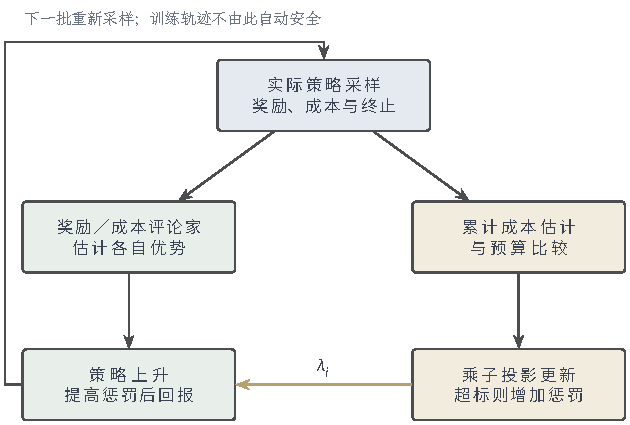
\includegraphics[width=106.659mm]{figures/10-reinforcement-learning/03-task-expansion-and-trustworthiness/tikz/rl-trustworthy-primal-dual.pdf}
  \caption{期望成本约束的两条反馈。奖励与成本优势共同推动策略更新，累计成本与预算的差推动乘子更新；这是一种求解循环，不是每次采样均满足约束的证书。}
  \label{fig:rl-trustworthy-primal-dual}
\end{figure}

\begin{theorem}[有限折扣CMDP的强对偶]
  \label{thm:rl-trustworthy-strong-duality}
  固定有限状态集、各状态非空有限动作集、转移核$T$和初态分布$\mu_0$，取$0\leq\gamma<1$。奖励$R(s,a)$、非负成本$c_i(s,a)$及有限预算$b_i$均固定且有界，$J$和$J_{c_i}$为从$\mu_0$启动的未归一化折扣期望。至少有一个满足全部预算的策略时，允许随机平稳策略的CMDP与占用度量线性规划等价，且
  \[
    \begin{aligned}
      \max_{\pi:\,J_{c_i}(\pi)\leq b_i}J(\pi)
        &=\min_{\bm{\lambda}\geq0}g(\bm{\lambda}),\\
      g(\bm{\lambda})
        &=\sum_i\lambda_i b_i+
          \max_\pi\left\{J(\pi)-\sum_i\lambda_iJ_{c_i}(\pi)\right\}.
    \end{aligned}
  \]
  原始最优解和有限维线性规划的对偶最优解存在。
\end{theorem}

证明以式~\eqref{eq:rl-trustworthy-cmdp-lp}~的占用量替代策略。可行占用集是非空、有界、闭多面体，线性目标有有限最优值，有限维线性规划强对偶因而给出相等的原始与对偶最优值。流守恒对应状态价值变量，成本不等式对应非负乘子；保留成本乘子并对占用流最大化，就得到定理中的$g$。这里使用的是原始问题非空且最优值有限的有限维线性规划强对偶，用于核对CMDP目标与乘子目标是否等价；相关基础可参考\BookChapterRef{chap:optimization}{卷1《数学准备：计算、分析与几何》“最优化”章}。

互补松弛还要求
$\lambda_i^\star(J_{c_i}(\pi^\star)-b_i)=0$：预算严格富余时乘子必须为0，预算恰好用尽时乘子却未必严格为正。强对偶依赖占用多面体的线性结构，不依赖任意神经网络参数集的凸性。参数化策略可能表示不了最优占用量，交替梯度也可能停在非全局解，因此上述定理不能直接当作神经网络训练的收敛保证。

乘子通过惩罚间接推动成本达标，\term{约束策略优化}（constrained policy optimization, CPO）则在旧策略附近直接限制一次更新的成本代理。代理沿用旧策略的状态分布，候选策略实际运行后却有新的状态分布，因此还需控制两者之差。令旧策略$\pi$与候选策略$\pi'$均为平稳Markov策略，对奖励或任一成本$f$定义
\[
  \begin{aligned}
    S_f(\pi',\pi)
      &=J_f(\pi)+\frac{1}{1-\gamma}
          \mathbb E_{s\sim d^\pi,a\sim\pi'}A_f^\pi(s,a),\\
    \epsilon_f
      &=\max_s\left|\mathbb E_{a\sim\pi'}A_f^\pi(s,a)\right|.
  \end{aligned}
\]
在共同MDP、共同初态和有界优势下，有
\begin{align}
  J(\pi')&\geq S_r(\pi',\pi)
      -\frac{2\gamma\epsilon_r}{(1-\gamma)^2}\overline D_{\mathrm{TV}},
      \nonumber\\
  J_{c_i}(\pi')&\leq S_{c_i}(\pi',\pi)
      +\frac{2\gamma\epsilon_{c_i}}{(1-\gamma)^2}\overline D_{\mathrm{TV}},
  \label{eq:rl-trustworthy-cpo-bound}\\
  \overline D_{\mathrm{TV}}
    &=\mathbb E_{s\sim d^\pi}
          \frac12\sum_a|\pi'(a\mid s)-\pi(a\mid s)|. \nonumber
\end{align}
式~\eqref{eq:rl-trustworthy-cpo-bound}~给回报下界和成本上界，方向不同，是因为收益需要不太低、成本需要不太高。其关键是占用变化界
$\|d^{\pi'}-d^\pi\|_1\leq
2\gamma\overline D_{\mathrm{TV}}/(1-\gamma)$。
性能差恒等式原本在$d^{\pi'}$下平均优势；将其换成$d^\pi$，用$\epsilon_f$乘上占用差，再除以$1-\gamma$，就得到上述误差项。若
$\mathbb E_{d^\pi}D_{\mathrm{KL}}(\pi'\|\pi)\leq\kappa$，Pinsker不等式和Jensen不等式进一步给出
$\overline D_{\mathrm{TV}}\leq\sqrt{\kappa/2}$。因此，精确求得
$S_{c_i}$加上误差余量不超过$b_i$，才直接推出下一策略成本达标。完整的界与CPO构造见原论文\scite{rl8-achiam2017-cpo}

实际CPO以样本优势、成本约束的一阶近似和KL的二阶近似求局部步，再用线搜索检查代理量；通常也没有精确估计$\epsilon_f$的全状态上界。只让线性化成本代理低于预算，至多得到仍带余项的成本界，不能据此省略余项而宣称严格可行。

Lagrangian PPO或SAC将乘子惩罚接入各自策略目标，仍继承对应采样和近似误差；SAC若包含熵奖励，所优化回报还发生了改变。奖励约束策略优化（reward constrained policy optimization, RCPO）采用便于学习的替代惩罚与多时间尺度更新，其收敛依赖替代惩罚和原约束的关系、步长及优化假设。任意换一个奖励，并不能由此推出原成本约束达标\scite{rl8-tessler2019-rcpo}

只有离线日志、不能继续试错时，乘子更新还面临另一项困难：候选策略改变状态访问分布，而原日志中的成本均值未必是候选策略的成本。COptiDICE（Offline Constrained Reinforcement Learning via Stationary Distribution Correction Estimation）沿用第~\ref{chap:rl-information}~章DICE的占用流校正，将固定策略评价扩展为带成本约束的占用优化。为看清其接口，仍取有限状态动作、时间不变MDP、$0\leq\gamma<1$、固定初态$\mu_0$及有界奖励和非负成本。日志训练样本$D$包含状态、动作、奖励、各项成本与下一状态，另需与目标启动条件相符的初态样本；令$d_D(s,a)$表示日志转移记录的状态动作抽样分布。它可以来自多种行为机制的混合，不要求已知某个单一行为策略$\beta(a\mid s)$。

把候选归一化占用写成$d(s,a)=d_D(s,a)w(s,a)$，其中$w\geq0$。与式~\eqref{eq:rl-information-dice}~评价固定目标策略不同，此处策略也待求解，因此先匹配状态流：对每个状态测试函数$v:S\to\mathbb R$，理想总体约束为
\begin{equation}
 \mathbb E_{(s,a)\sim d_D,\,s'\sim T(\cdot\mid s,a)}
   \left[w(s,a)\{v(s)-\gamma v(s')\}\right]
   =(1-\gamma)\mathbb E_{s_0\sim\mu_0}v(s_0).
 \label{eq:rl-trustworthy-coptidice-flow}
\end{equation}
全部$v$的约束对应式~\eqref{eq:rl-trustworthy-cmdp-lp}~的状态流守恒，使加权后的记录可解释为某个候选策略的折扣访问，而非任意提高高奖励样本的权重。方法在归一化奖励目标$\mathbb E_{d_D}[wR]$中减去$\eta\mathbb E_{d_D}f(w)$，其中$\eta>0$，$f$为满足$f(1)=0$的严格凸可微函数，以惩罚占用量过度偏离日志分布；成本约束配非负乘子，状态流配状态势函数，经对偶化用转移样本学习$w$。这一占用正则化会改变无正则CMDP的优化目标，不能将两者的最优回报直接等同。

只代入经验均值$\mathbb E_{d_D}[wc_i]$仍可能低估成本。COptiDICE进一步对成本作稳健的上侧估计：将初态样本与$(s,a,s')$转移记录组成的联合样本律作为扰动对象，限制其相对经验联合律的KL距离不超过$\epsilon_{\mathrm{rob}}\geq0$，并要求扰动后的初始分布、转移条件律及$\widetilde p(s,a)w(s,a)$仍满足同一占用流方程。随后求这些兼容分布下加权成本$\mathbb E_{\widetilde p}[wc_i]$的上确界，再将上侧估计经非负乘子接入策略优化。原论文的对偶成本目标因此含状态势函数的流残差修正，不能替换为只对状态动作边缘分布任取KL球的$\mathbb E[wc_i]$。$\eta$控制占用正则强度，$\epsilon_{\mathrm{rob}}$控制成本扰动范围，两者具有不同作用。由于这里$J_{c_i}$未归一化，归一化占用下的成本上侧估计应与$(1-\gamma)b_i$比较，不能直接与$b_i$比较\scite{rl8-lee2022coptidice}

获得满足相应流约束的占用比后，有限动作情形可按
\begin{equation}
 \pi_w(a\mid s)=
   \frac{d_D(s,a)w(s,a)}
        {\sum_{a'\in\mathsf A(s)}d_D(s,a')w(s,a')},
 \qquad \sum_{a'}d_D(s,a')w(s,a')>0
 \label{eq:rl-trustworthy-coptidice-policy}
\end{equation}
恢复候选策略。式~\eqref{eq:rl-trustworthy-coptidice-policy}~归一化的是日志状态动作质量乘占用比，不是要求先恢复原行为概率。例如只有一个自循环状态、两个动作$L,R$、初态就在该状态时，取$d_D=(3/4,1/4)$和$w=(1/3,3)$，得到候选占用$(1/4,3/4)$，其总质量为1，满足任意$0\leq\gamma<1$下的状态流；恢复的动作概率也为$(1/4,3/4)$。这是抽取步骤的手算示例，不是算法在某个基准上学得的结果。连续动作通常用$\mathbb E_{d_D}[w\log\pi_{\bm\theta}(a\mid s)]$作加权行为克隆，所提取策略还会增加函数逼近与拟合误差。

原总体推导以日志分布充分支持为条件；支持不全时只能在已覆盖的经验CMDP中求解。分母为0的状态可另选合法策略，但日志没有据此识别这些选择的回报或成本；$d_D(s,a)=0$处也不能靠有限权重创造正占用。还须存在受日志支持且满足所选成本稳健约束的候选方案，否则惩罚和乘子都不能创造缺失的可行策略。在精确求解相应稳健问题时，成本上界针对所声明的联合扰动集；真实运行律是否被该集合覆盖须另有依据，KL半径本身不构成普遍的有限样本安全保证。采样、流匹配函数类、比率优化与策略抽取误差仍需核查，最终固定策略的成本也仍须按第~\ref{sec:rl-trustworthy-inference}~节的评价协议取证。

理想占用规划的全局最优与强对偶、近似更新的误差控制、最终策略的原成本验证，至此已有各自依据。它们仍未约束每条训练轨迹：即使输出策略平均成本达标，先前探索也可能违反安全要求。要约束整个学习过程，还须明确其事件或硬安全标准。

% Outline: 8.4.2
\subsection{轨迹事件概率约束下的安全学习}
\label{sec:rl-trustworthy-chance}

第二类约束直接盯住“出事”这件事本身，而不是出事造成的平均成本。如果要求直接限制整次导航出事的可能性，平均碰撞成本就不是所需指标。例如规格要求发生任意碰撞的概率不超过1\%。设$E_t$为动作$t$导致碰撞的事件，定义
\[
  F_H=\bigcup_{t=0}^{H-1}E_t,\qquad
  \mathbb P_\pi(F_H)\leq\varepsilon.
\]
这就是\term{机会约束}（chance constraint）：允许违约发生，但指定事件的概率须不超过阈值。阈值来自任务要求，时域$H$决定哪些动作纳入事件。$\mathbf1\{F_H\}$不区分一次与多次碰撞，也不区分损坏1个与100个部件，因此相同失败概率仍可能对应不同事故成本。

首次碰撞之后再次碰撞，不应重复计入“至少发生一次”的概率。为保存这段历史，把失败标记加入状态：令$z_0=0$、$z_t\in\{0,1\}$，并递推
$z_{t+1}=z_t\lor\mathbf1\{E_t\}$。若原系统和碰撞判定在状态、动作与后继状态上是马尔可夫的，则$(s_t,z_t)$也是马尔可夫状态，且
$\mathbb P_\pi(F_H)=\mathbb E_\pi z_H$。
对于以状态集合$\mathcal B$表示的危险区域，也可令$z_0=\mathbf1\{s_0\in\mathcal B\}$，将初始失败纳入事件；两种起始约定不能混用。

固定时间相关策略$\pi_t$后，从终端标记向前求期望，即可得到概率价值$v_t(s,z)$：
\begin{align}
  v_H(s,z)&=z,\nonumber\\
  v_t(s,z)&=\sum_a\pi_t(a\mid s,z)
       \sum_{s'}T(s'\mid s,a)
         v_{t+1}\bigl(s',z\lor e(s,a,s')\bigr),
  \label{eq:rl-trustworthy-probability-value}
\end{align}
其中$e(s,a,s')$为本步事件指示量。按$t=H-1,\ldots,0$回传，最后对$\mu_0$平均$v_0(s,0)$，就得到整回合失败概率；若计入初始危险状态，则改为平均$v_0(s,z_0(s))$。这里求的是事件概率，不是折扣回报，因此不应额外乘奖励任务的折扣因子。在$z_0=0$的约定下，也可定义首次失败成本
$k_t=\mathbf1\{z_t=0,z_{t+1}=1\}$，则$\sum_tk_t=z_H$；普通碰撞次数之和一般不等于$z_H$。

把单步要求接成回合要求，只需同一概率空间上的事件关系。取正整数时域$H$和任意可测事件$E_0,\ldots,E_{H-1}$，并集界给出
\[
 \mathbb P(F_H)=\mathbb P\left(\bigcup_{t=0}^{H-1}E_t\right)
 \leq\sum_{t=0}^{H-1}\mathbb P(E_t).
\]
因此，非负预算若满足$\mathbb P(E_t)\leq\varepsilon_t$且$\sum_t\varepsilon_t\leq\varepsilon$，就支持整回合失败概率不超过$\varepsilon$。这个结论不要求各步事件独立，用途是把可检查的单步概率预算接到回合事件；相关概率工具可参考\BookChapterRef{chap:random-variables}{卷2《数学准备：概率、因果与决策》的“随机变量与概率基础”章}。

并集界将各步事件概率相加，一条轨迹上的多次碰撞可能被重复计入，所以界可能保守。若预算针对尚未失败时的下一步，则应改用存活条件。令
$S_t=\bigcap_{j<t}E_j^c$，在$\mathbb P(S_t)>0$时定义
$q_t=\mathbb P(E_t\mid S_t)$，则由条件概率乘法
\[
  \mathbb P(F_H)=1-\mathbb P(S_H)
       =1-\prod_{t=0}^{H-1}(1-q_t).
\]
取条件预算$\beta_t\in[0,1]$，则$q_t\leq\beta_t$推出
$\mathbb P(F_H)\leq1-\prod_t(1-\beta_t)\leq\sum_t\beta_t$。
乘积来自连续存活的条件概率链，不来自事件独立性。$q_t$已对所有存活历史求平均；要求每个存活历史下的条件概率都不超过$\beta_t$，是更强的充分条件。某时刻存活概率若为0，整回合失败概率已经是1，无须再定义后续条件概率。因此，无条件$\mathbb P(E_t)$、存活条件$q_t$和特定状态下的概率，不能共用同一预算解释。

教学计算中，若每步给定存活后的碰撞概率都是0.01，则$H=10$时整回合概率为
$1-0.99^{10}\approx0.0956$，$H=100$时为
$1-0.99^{100}\approx0.6340$。这两个数不需要额外假设各$E_t$独立，因为条件概率已被直接给定。若要求100步整回合不超过0.01，并且均匀分配条件预算，每步应满足
$\beta\leq1-0.99^{1/100}\approx0.00010050$。
图~\ref{fig:rl-trustworthy-events}~另将多个训练回合括在一起：最终策略单回合的$F_H$与训练期间任一回合出事的事件，具有不同样本空间和时域。

\begin{figure}[htbp]
  \centering
  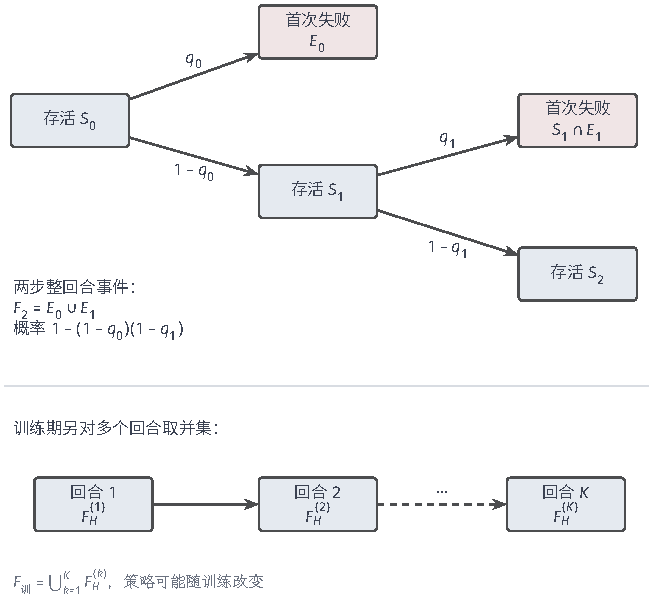
\includegraphics[width=110.652mm]{figures/10-reinforcement-learning/03-task-expansion-and-trustworthiness/tikz/rl-trustworthy-events.pdf}
  \caption{单步事件、整回合事件与整个学习过程事件。树在首次失败后合并成终止分支；下方回合可以使用不同策略，不能直接套用固定策略独立同分布的频率模型。}
  \label{fig:rl-trustworthy-events}
\end{figure}

事件定义明确后，学习方法取决于能否取得模型。直接采样时，每回合记录一次$z_H$，以均值估计概率，再用轨迹得分
$z_H\sum_t\nabla\log\pi(a_t\mid I_t)$估计概率梯度，并据此作拉格朗日约束更新。稀有事件使失败概率的相对误差更难控制，概率梯度也可能主要由极少数失败回合贡献；一批全为零的事件标记会使这份样本的梯度估计为0，但这只是没有观测到失败，不是安全证明。

模型已知时，可由式~\eqref{eq:rl-trustworthy-probability-value}~评价候选，或在时间和失败标记增广状态上优化期望终端成本，单次稠密评价代价为$O(H|S|^2|\mathsf A|)$。两种方法都需要完整事件标记；超时截断后未记录的事故，不能被当作没有发生。

如果不同后继状态需要不同风险余量，还可将剩余允许概率作为决策状态。到达尚未失败的$(t,s)$，剩余预算为$b\in[0,1]$，候选动作$a$的立即失败概率为$p_f(s,a)$，即对$e(s,a,s')=1$的后继转移概率求和。给未失败后继分配$b(s')\in[0,1]$，用全概率将立即失败和未来失败分开：
\begin{equation}
  p_f(s,a)+
    \sum_{s':\,e(s,a,s')=0}T(s'\mid s,a)b(s')\leq b.
  \label{eq:rl-trustworthy-risk-budget}
\end{equation}
\begin{samepage}
一个两分支计算可以说明后继预算的含义。设动作以0.1概率立即失败，以0.3和0.6概率分别到达两个安全后继$s_1,s_2$，这三项概率之和为1。给后继分配$b(s_1)=0.2$、$b(s_2)=0.05$，若两个后继的后续策略分别保证失败概率不超过这些预算，则整个后续失败概率的上界为
\[
  0.1+0.3\times0.2+0.6\times0.05=0.19.
\]
当前预算$b=0.2$时，这项分配通过当前一步的预算检验；整体可行还要求两个后继预算均可实现。到达$s_1$后，0.2是条件于已经到达该状态且此前未失败的后续概率上限；到达$s_2$后，相应上限为0.05。二者先经到达概率加权，才与立即失败概率一起接受当前预算检验，因此不能都用$0.2-0.1$作为同一个“剩余概率”。
\par
\end{samepage}

式\eqref{eq:rl-trustworthy-risk-budget}右侧的$b$限制的是条件于当前尚未失败状态的整个后续失败概率。选择满足该式且未来回报最高的动作与预算分配，到达$s'$后携带$b(s')$继续；最后一步后未来失败概率为0，向后归纳即可证明总概率不超过$b$。随机化动作时，还须对动作取平均并保留选定分支的预算。连续预算增加状态维度，网格化则带来规模和近似误差；随意从$b$减去一个“风险分数”没有对应的概率依据。

直接处理事件概率困难时，可以考虑CVaR的保守替代，但需要让损失编码与失败事件对应。令$X(\tau)>0$恰好表示失败，例如轨迹上最大的边界超出量。$X$可积时，有
\[
  \operatorname{CVaR}_{1-\varepsilon}(X)\leq0
  \quad\Longrightarrow\quad
  \operatorname{VaR}_{1-\varepsilon}(X)\leq0
  \quad\Longrightarrow\quad
  \mathbb P(X>0)\leq\varepsilon.
\]
第一个箭头依据尾部均值不小于分位点，第二个依据分位点定义；CVaR因而同时约束尾部严重程度，通常比原事件要求更强。反向不成立：以0.99概率取$X=-1$、以0.01概率取$X=100$，满足$\varepsilon=0.05$的机会约束，但最差5\%均值为
$(0.01\times100-0.04)/0.05=19.2>0$。若直接令$X=\mathbf1\{F_H\}$，则
$\operatorname{CVaR}_{1-\varepsilon}(X)=\min(1,p/\varepsilon)$；
把这一非负量限制为0，要求的是$p=0$，远强于原机会约束。采用替代目标前，须检查损失编码是否保留了所需事件含义，不能只匹配CVaR的名称和分位水平。

表~\ref{tab:rl-trustworthy-chance-methods}~将所需模型或记录与方法对应：完整回合支持直接采样，可信模型支持概率递推和预算分配，违约量的尾部分布支持CVaR替代。选择的既是求解手段，也可能是一个更保守的约束，因此须同时核对模型、采样条件和行为含义。

\begin{table}[htbp]
  \centering
  \begin{tabularx}{\linewidth}{@{}>{\raggedright\arraybackslash}p{21mm}XX@{}}
    \toprule
    方法 & 所需模型与记录 & 计算及主要边界 \\
    \midrule
    整回合采样 & 完整事件标记、固定时域与初态协议 & 每回合一个Bernoulli量；罕见事件样本少 \\
    概率价值递推 & 转移模型、时间、已失败标记 & 逐阶段备份；模型漏掉危险转移即失效 \\
    风险预算分配 & 上述模型、剩余预算及后继分配 & 增广预算空间；可行分配未必存在 \\
    CVaR替代 & 可积违约量及其尾部分布 & 同时限制尾部严重程度；通常更保守 \\
    \bottomrule
  \end{tabularx}
  \caption{机会约束的四种处理方式。它们分别解决估计、规划或保守替代问题，不能用相同数值阈值互相替换。}
  \label{tab:rl-trustworthy-chance-methods}
\end{table}

\begin{samepage}
若学习过程有$K$回合，记第$k$回合失败事件为$F_H^{(k)}$，训练期事件是
$F_{\text{训}}=\bigcup_{k=1}^KF_H^{(k)}$。即使每个训练回合都有概率上界$\varepsilon_k$，也只能直接得到
$\mathbb P(F_{\text{训}})\leq\sum_k\varepsilon_k$；自适应训练中可先对过去训练历史给条件上界，再用全期望与并集界。仅验证训练结束后的策略，完全没有约束先前探索使用的策略序列。
\par
\end{samepage}

% Outline: 8.4.3
\subsection{逐步与逐轨迹硬要求下的安全学习}
\label{sec:rl-trustworthy-hard-safety}

逐步与逐轨迹硬要求直接排除声明范围内的违规行为。这时候逐时刻检查“当前是否合法”是不够的。若要求任何时刻都不越界，检查当前机器人位置仍合法还不够：高速逼近边界且制动力不足时，即使此刻仍在界内，下一步也可能已经没有任何安全动作。硬安全需要的是往前看一步，找到那些“进去之后还能一直安全待下去”的状态。对已知离散系统
$\bm{x}_{t+1}=f(\bm{x}_t,\bm{u}_t,\bm{w}_t)$，用任务规格定义允许状态集$\mathcal X$，用执行器能力定义输入集$\mathcal U(\bm{x})$，用运行协议或模型误差界定义扰动集$\mathcal W(\bm{x},\bm{u})$。

\begin{definition}[控制不变集与可恢复集]
  \label{def:rl-trustworthy-invariance}
  对已知离散动力学$\bm{x}_{t+1}=f(\bm{x}_t,\bm{u}_t,\bm{w}_t)$，固定允许状态集$\mathcal X$、各状态可执行输入集$\mathcal U(\bm{x})$及输入确定后的允许扰动集$\mathcal W(\bm{x},\bm{u})$。
  集合$\mathcal K\subseteq\mathcal X$是鲁棒控制不变的，如果每个$\bm{x}\in\mathcal K$都有输入$\bm{u}\in\mathcal U(\bm{x})$，使所有
  $\bm{w}\in\mathcal W(\bm{x},\bm{u})$对应的后继状态仍在$\mathcal K$。
  一个从$\mathcal K$内选择这类输入的规则称为备份策略。
  给定备份不变集和非负整数步数$N$，可恢复集由那些存在非预见控制策略、能在所有允许扰动下始终留在$\mathcal X$并于至多$N$步进入$\mathcal K$的状态组成；非预见指本步输入只能使用已观察历史，不能使用尚未发生的扰动。
\end{definition}

定义中的量词顺序是“存在同一个输入，使所有允许扰动都安全”，不是针对每个扰动事后另选输入。允许状态集未必满足这一条件，可恢复集也随输入限幅、扰动范围和可用时间改变。若还要求整条轨迹成本不超过$B$，须保留剩余预算
$b_{t+1}=b_t-c_t$、$b_0=B$，并在增广状态$(\bm{x}_t,b_t)$上要求$b_t\geq0$及未来可行。折扣预算对应扣减$\gamma^tc_t$，或采用一致的相对时刻预算递推；不能用期望成本评论家替代每条轨迹的余额。

\begin{theorem}[安全集的一步封闭性保证]
  \label{thm:rl-trustworthy-invariance}
  考虑离散系统
  \[
    \bm{x}_{t+1}=f(\bm{x}_t,\bm{u}_t,\bm{w}_t).
  \]
  固定集合$\mathcal K\subseteq\mathcal X$、可执行输入集$\mathcal U(\bm{x})$和允许扰动集$\mathcal W(\bm{x},\bm{u})$。假定动力学$f$已知，实际状态可准确获得，初态$\bm{x}_0\in\mathcal K$，实际扰动始终在声明集合内。若每个$\bm{x}\in\mathcal K$的可行保护输入集合
  \[
    \begin{aligned}
      \mathcal U_{\mathcal K}(\bm{x})
        =\bigl\{\bm{u}\in\mathcal U(\bm{x}):\ &
          f(\bm{x},\bm{u},\bm{w})\in\mathcal K,\\
        &\text{对所有 }\bm{w}\in\mathcal W(\bm{x},\bm{u})\bigr\}
    \end{aligned}
  \]
  非空，且执行器在每步实际施加其中一个输入，则每条允许扰动轨迹都满足$\bm{x}_t\in\mathcal K$，$t\geq0$。
\end{theorem}
\begin{proof}
  固定任意满足扰动集合限制的轨迹。初始条件给出$\bm{x}_0\in\mathcal K$，这是归纳起点。
  假设在某个$t$有$\bm{x}_t\in\mathcal K$。集合非空保证能够选择
  $\bm{u}_t\in\mathcal U_{\mathcal K}(\bm{x}_t)$；按定义，对所有允许扰动，特别是实际发生的$\bm{w}_t$，
  \[
    \bm{x}_{t+1}=f(\bm{x}_t,\bm{u}_t,\bm{w}_t)\in\mathcal K.
  \]
  归纳步成立，故所有有限$t$都有$\bm{x}_t\in\mathcal K$。由于起初固定的轨迹任意，结论对每条允许扰动轨迹均成立。
\end{proof}

归纳证明把每步的全称保持条件传到整条轨迹，因此每项前提都影响结论。$\mathcal U_{\mathcal K}$若为空，就不存在满足要求的保护输入；状态判断若有误，所选动作可能不属于真实状态的可行集合；扰动越界或未建模延迟也会破坏一步封闭性。状态只能估计为集合$\widehat{\mathcal X}_t$时，须让同一个输入对全部可能真实状态和允许扰动有效，并另行保证真实状态确实在估计集合内。

定理~\ref{thm:rl-trustworthy-invariance}~也给出了执行检查：先有已验证不变集$\mathcal K$，再检查候选输入是否使全部允许后继仍在$\mathcal K$内。这样的数学条件及其成立依据称为\term{安全证书}（safety certificate），也就是可据以检验行为的证明条件。算法~\ref{alg:rl-trustworthy-filter}~使用这一不变集证书；屏障函数和预测过滤器则提供构造或检验保持条件的其他方式。距离最小的修正只用于尽量保留候选意图，并不产生安全性；只有保护输入集合非空且距离最小值取到时，算法才能要求最近点。若最小值不取到或求解器未在时限内返回经验证的可行点，只能改用当前仍满足同一保持条件的备份；集合为空或备份也未通过当前检查时，须报告保证失效。

\begin{algorithm}[带可行性检查的安全过滤]
  \label{alg:rl-trustworthy-filter}
  \begin{algorithmic}[1]
    \Require 候选策略、有效状态估计集合、动力学及误差集合、已验证不变集$\mathcal K$及其一步保持条件、可用备份
    \For{每个执行时刻$t$}
      \State 取得候选动作$\bm{u}^{\text{候}}_t$，更新状态估计集合
      \State 按定理~\ref{thm:rl-trustworthy-invariance}~构造保护输入集合：同一输入须使所有可能真实状态在所有允许扰动下的后继都留在$\mathcal K$
      \State 若候选动作在集合中，直接使用；否则，仅在最近点存在且求解器及时返回时使用距离最小的可行输入
      \State 若最近点不存在或优化超时，改用经过当前一步保持检查的备份；若集合为空或备份也不可行，报告保证失效并触发预设应急机制
      \State 执行实际动作，记录候选、实际动作、干预原因和后继状态，反馈给学习器
    \EndFor
  \end{algorithmic}
\end{algorithm}

过滤优化超时后，备份能否接管仍要在当前状态检查。应急停止只有满足相同模型和可行性条件时，才是证明中的安全输入；若已经没有安全制动距离，“优化失败就刹车”不能恢复已丢失的保证。图~\ref{fig:rl-trustworthy-filter}~因而将模型、状态估计和备份直接送入保护模块，并把实际动作反馈给学习器。

\begin{figure*}[t]
  \centering
  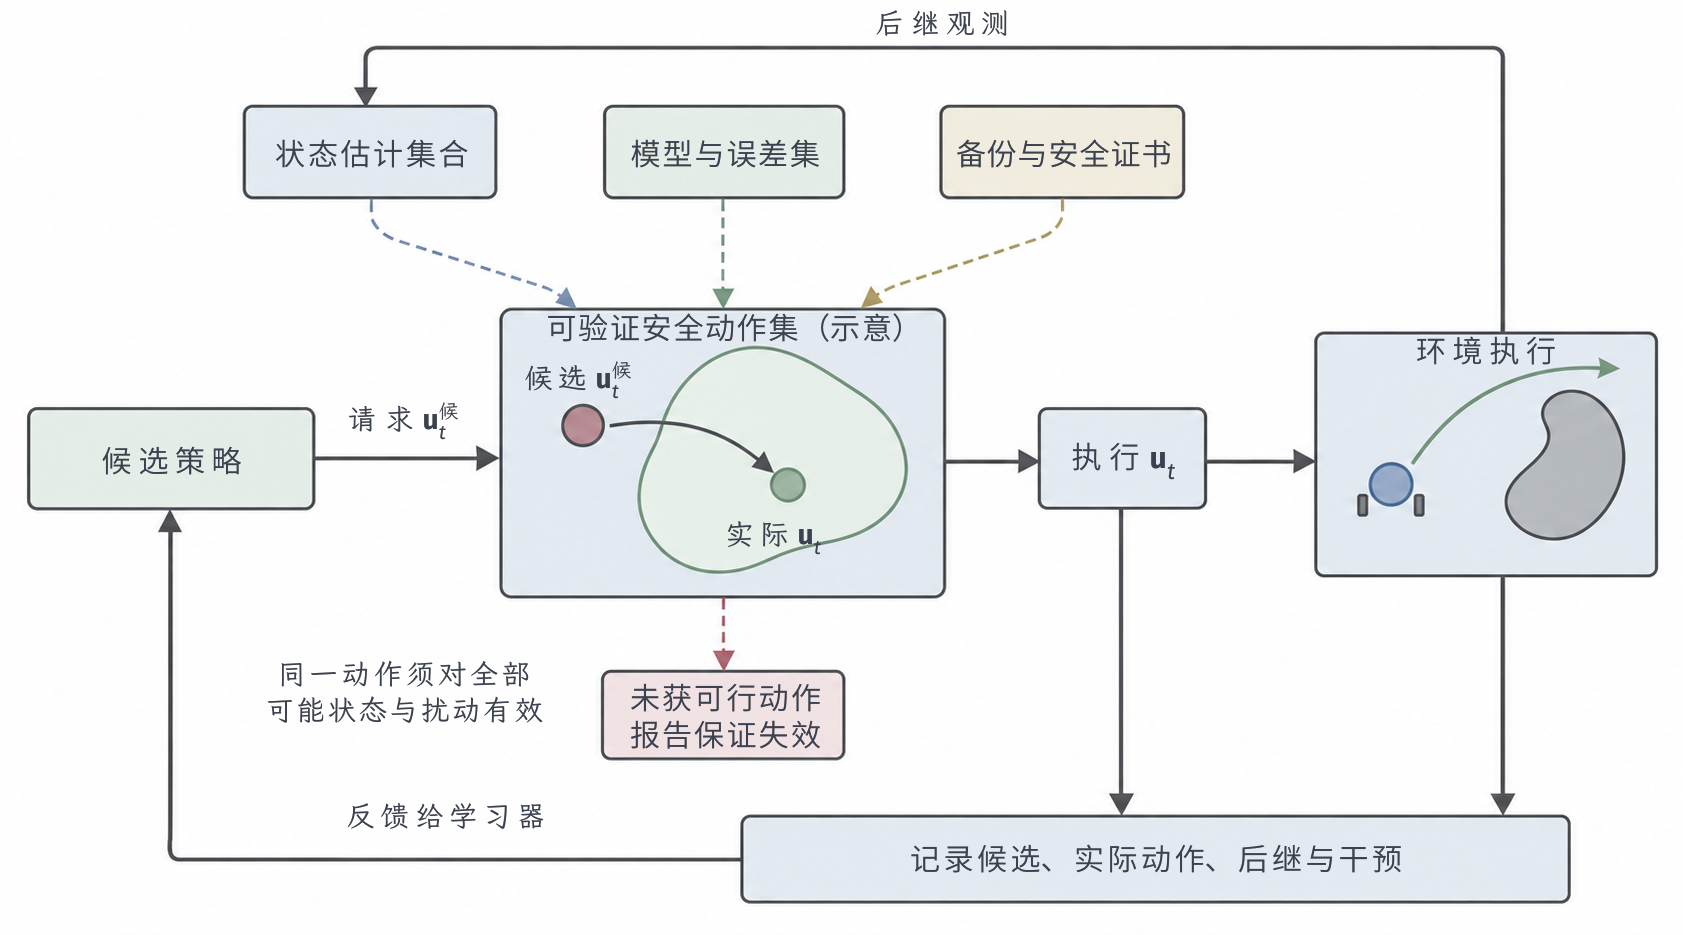
\includegraphics[width=157.400mm]{figures/10-reinforcement-learning/03-task-expansion-and-trustworthiness/generated/rl-trustworthy-filter/figure.png}
  \caption{保护器对控制动作的筛选与执行。实线连接候选动作、实际动作、环境和执行记录，虚线给出保护判断依赖的状态估计、模型与证书。动作区域仅为集合示意，不表示凸性、最近点存在或精确投影；未取得可验证动作时报告保证失效。右侧避障场景仅示意执行，评价仍须说明保护是否启用及保证针对哪个组合系统。}
  \label{fig:rl-trustworthy-filter}
\end{figure*}

离散动作下，可以屏蔽不满足一步保持条件的动作。若安全动作上的候选策略总质量为正，就将这些动作的原概率按该总质量归一化；若总质量为0，例如确定性候选只提出危险动作，则改用预先声明且经当前保持条件验证的备份分布。安全动作集为空，或备份分布不再受其支持时，屏蔽规则没有可执行的安全选择，必须报告保证失效。任务规格若含历史要求，屏蔽状态还可能包括表示规格进展的任务自动机或历史标记。普通\term{动作屏蔽}（action masking）只删除“向墙内移动”等即时非法动作，未必保留未来安全；按安全规格构造的屏蔽则在抽象模型上维护允许后继，其保证取决于抽象是否覆盖真实系统\scite{alshiekh2018shielding}

连续输入下，若可行集非空且最近点存在，可在其中找距离候选最近的动作，以尽量保留候选意图：
\[
  \min_{\bm{u}\in\mathcal U_{\mathcal K}(\bm{x})}
          \|\bm{u}-\bm{u}^{\text{候}}\|^2.
\]
教学系统$x_{t+1}=x_t+u_t+w_t$取$\mathcal K=[0,1]$、
$u_t\in[-0.2,0.2]$、$w_t\in[-0.05,0.05]$。鲁棒一步条件为
$0.05-x_t\leq u_t\leq0.95-x_t$。在$x_t=0.96$时，候选$u_t=0.1$会使最坏后继达到1.11；与输入限幅取交后，可行集为$[-0.2,-0.01]$，投影得到$u_t=-0.01$，后继范围为$[0.90,1.00]$。投影将朝边界的正动作改为负动作，是因为可行区间已计入最坏扰动；后继范围的显式计算才是保持安全的依据。

为了把“始终留在安全区”这一几何条件变成算法可以逐次检查的输入约束，\term{控制屏障函数}（control barrier function, CBF）用$h(\bm{x})\geq0$表示允许区域（状态安全当且仅当$h$非负），并限制输入使$h$不变为负。离散时间须检查
$h(f(\bm{x},\bm{u},\bm{w}))\geq0$对允许扰动成立，或者使用能够推出这一条件的更强不等式。连续时间控制仿射系统
$\dot{\bm{x}}=\bm{f}(\bm{x})+\bm{g}(\bm{x})\bm{u}$则常使用
\[
  \nabla h(\bm{x})^\top
       \bigl(\bm{f}(\bm{x})+\bm{g}(\bm{x})\bm{u}\bigr)
        \geq-\alpha_h(h(\bm{x})).
\]
其中$h$连续可微，$\alpha_h$是适当的扩展类$\mathcal K$函数，即连续、严格递增且$\alpha_h(0)=0$。不等式限制$h$下降的速度，使它在边界处不能继续朝负值方向穿越。在边界处$\nabla h\neq0$、声明时域内闭环解存在且唯一、输入约束下不等式始终可行、实际反馈满足不等式且初态在集合内等条件下，比较原理支持正向不变性，即闭环轨迹在声明时域内留在允许集合。它在此用于限制训练所得策略请求的动作；相关控制基础可参考\BookChapterRef{chap:policy-realization-and-control}{卷2《数学准备：概率、因果与决策》“策略的实现与轨迹控制”章}。

控制仿射性使输入以线性形式出现在约束中，常可和二次投影目标组成\term{二次规划}（quadratic program, QP）。输入饱和或多个约束冲突仍可能使QP不可行。连续时间不等式只约束所分析的连续闭环，采样间隔、执行延迟和模型误差还须通过余量或离散分析另行覆盖\scite{rl8-ames2017-barrier}

\term{预测安全过滤器}（predictive safety filter）把检查延伸到未来控制计划：预测时域内状态和输入都满足约束，末端进入已有备份能够维持的不变集，优化目标则可优先保留当前候选动作\scite{rl8-wabersich2021-filter}
鲁棒版本须使用反馈计划或误差管束；管束保存的是各步所有允许状态，而非一条标称避障轨迹。若执行一步后真实状态仍在旧的可行管束内，下一时刻就可向前平移旧计划，并在末端接上备份控制。这给出递归可行性的依据，即本次可行能为下一次留下可行方案。

误差集合突然扩大、终端集失效、状态估计离开管束或求解未按时完成，都可能破坏这一依据。预测步数、状态维度和非线性误差传播还决定在线代价，因此采用“MPC过滤”并不免除模型覆盖、可行性和求解时限的检查。

过滤维持当前可行性，恢复控制则把系统带回已验证区域，并须在返回过程中保持约束。停止学习任务、返回安全种子可以是整体方案的一部分。近期安全复位研究联合建模到达复位区域与避开危险；无人干预学习因此还要检查回合之间的重置，而不只检查单回合动作。这扩大了保证时域，也增加了复位路径、时间和控制能力的要求，不能假定复位天然安全或没有代价\scite{rl8-begzadic2025-reset}

上述过滤依赖动力学，模型未知时通常要从已知安全种子区域或备份控制开始，用保护器实际执行后取得的状态、实际动作及后继状态记录缩小模型误差集，再扩展可验证区域。高斯过程（Gaussian process, GP）可以预测均值与不确定区间；但证书需要真实动力学在声明状态输入范围及所有取证时刻上，以至少$1-\delta$的概率同时被模型集合覆盖。联合覆盖通常依赖函数正则性、噪声假设、置信参数及对自适应采样的控制。稳定性证书与GP误差界相结合的安全学习依赖这些条件，单有预测方差还不能支撑安全声明\scite{rl8-berkenkamp2017-safe}

记联合模型覆盖事件为$C_{\mathrm{cov}}$，结论可分两步表述：“在$C_{\mathrm{cov}}$上，过滤器按不变性条件保持安全；取证程序满足$\mathbb P(C_{\mathrm{cov}})\geq1-\delta$。”前一步是条件于模型覆盖的逻辑保证，后一步才是统计覆盖。单个点的95\%预测区间不能替代整条闭环轨迹的联合事件。扰动若有无界支持，也不能无条件假定所有时刻均在有界集合内；有限时域高概率覆盖与无限时域逐轨迹保证须分别论证。

多机器人共享狭窄通道时，两个机器人若都假定“对方会等待”，各自可能有可行计划，联合执行却会相撞。团队保证因而还须核对联合输入约束、通信延迟和参与者的建模承诺。去中心化过滤只有在局部假设相容、联合可行域非空且执行时可读取的观测、状态与消息符合证明条件时，才可能支持团队安全；个体QP各有一个解不够。参与者响应模型仍由第~\ref{chap:rl-multi-agent}~章提供。

% Outline: 8.5
\section{可靠性评价与保证}
\label{sec:rl-trustworthy-evidence}

前面几节解决的是“怎样求出一个试图满足要求的策略”，但求解器在训练中优化了某个代理目标，不等于交付对象真的满足原要求；受保护系统长期无事故，也可能只是保护器在起作用，无法说明移除保护后的表现。所以还需要一个独立于训练的取证环节：预先固定取证协议，再依据评价样本或模型证明，估计各项指标落在什么范围、保证覆盖到哪里。图~\ref{fig:rl-trustworthy-validation}~显示这一依赖：运行条件改变时，旧成功次数是否仍可使用，须先重新核对协议。

\begin{figure*}[t]
  \centering
  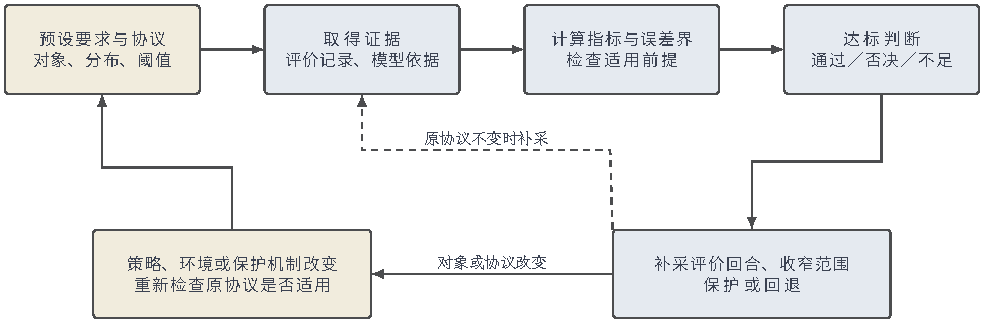
\includegraphics[width=166.617mm]{figures/10-reinforcement-learning/03-task-expansion-and-trustworthiness/tikz/rl-trustworthy-validation.pdf}
  \caption{运行记录、性能估计与可靠性判断之间的依赖。判断可以触发补充取证、收窄范围、保护或回退；原协议不变时，虚线返回允许补采记录。评价对象、保护配置或协议改变时，先重新核对协议，再取证和估计。流程本身不替代统计覆盖或模型证明。}
  \label{fig:rl-trustworthy-validation}
\end{figure*}

% Outline: 8.5.1
\subsection{确定验证协议并取得证据}
\label{sec:rl-trustworthy-protocol}

取证的第一步不是算统计量，而是把“这次运行到底在检验什么”固定下来。导航验证可以改变初始位置、训练种子或摩擦条件，但三种变化回答不同问题。固定策略从不同位置启动，评价其运行分布；换种子重新训练，评价学习规则产生的训练模型的变化；同一系统换摩擦条件，检查声明运行范围。未经区分就汇总成功率，会把策略、初态与环境三方面的影响混在一起，无法归因。

协议首先按保证对象冻结不同内容。评价固定策略或策略与保护层的组合时，冻结交付策略和保护器版本；评价固定学习规则的重复训练时，冻结训练流程、训练记录的生成与采样机制、训练样本预算、种子分布以及输出策略的验收规则，单次训练产生的输出策略本身是随机对象，不能事先冻结。随后再确定统计单位、初态与环境抽样分布、时域和终止规则、允许扰动与参与者、失败判定、回报与成本阈值及置信要求。这些约定决定怎样把一次运行或一次完整训练转成证据。碰撞若定义为“机身越过边界”，仅记录报警就不足以判定事件。恢复时间也须约定起点和恢复集合；观察结束仍未恢复，意味着真实恢复时间尚不完整，应按删失或超时规则处理，不能删去这些回合后计算平均值。

表~\ref{tab:rl-trustworthy-evidence-sources}~对应证据来源与可支持结论。模型证明覆盖显式模型的全部允许情况，运行试验则有助于发现实际系统中的模型遗漏。两者可以互补，但模型前提和试验抽样范围都须保留在结论中。

\begin{table*}[t]
  \centering
  \begin{tabularx}{\linewidth}{@{}>{\raggedright\arraybackslash}p{23mm}XXX@{}}
    \toprule
    证据来源 & 统计单位与可控条件 & 可支持结论 & 关键缺口 \\
    \midrule
    重复训练 & 一次完整训练；算法、预算、种子分布固定 & 输出策略指标分布、训练失败概率 & 不能只挑最好种子报告 \\
    固定策略重复运行 & 一回合；策略和运行协议冻结 & 协议分布下的回报、成本和事件概率 & 回合独立性、有效样本量 \\
    压力测试 & 指定极端场景或攻击；权限固定 & 已测条件下的失效及响应 & 不直接给常态运行失败频率 \\
    已有日志 & 日志中的回合；行为机制可追溯 & 覆盖与校正条件下的离线评价 & 漏报事件、选择性记录、支持不足 \\
    形式化模型分析 & 模型中的状态、轨迹或扰动集合 & 前提成立时的全称性质 & 真实系统是否满足抽象与误差前提 \\
    \bottomrule
  \end{tabularx}
  \caption{取证方式与保证对象的对应关系。重复训练的一条学习曲线不是一次固定策略运行，主动挑选的极端情况也不是从日常运行分布随机抽到的回合。}
  \label{tab:rl-trustworthy-evidence-sources}
\end{table*}

要避免选择偏差，最终检验使用的任务与运行记录也须与开发使用的任务及训练记录区分。任务、攻击和训练种子一旦用于更新策略，就不再是未使用的测试证据；验证集若用于反复挑选策略，也已参与选择。可以分开开发、策略选择和最终验收，或事先使用对整个候选类同时有效的界。只留出随机种子仍不够：困难地形若被反复用于调节保护阈值，这些地形上的运行反馈已经参与方案调整。对预先冻结的候选，独立评价样本支持相应的固定候选风险界；从同一批样本中选择候选时，须让界同时覆盖预定候选类，或在选择后另取独立评价样本。相关原则可参考\BookChapterRef{chap:trust-reliability}{卷3《基础、理论与可信性》“可靠性”章}。

为还原执行机制，每回合须保留初始条件、请求动作、实际动作、奖励、损失、成本、事件标记、接管时刻和恢复时间。失败后的运行记录有助于诊断后果和恢复，不应因回合“已经失败”而从日志消失。干预率还须固定分母：被替换动作占总动作的比例，和至少接管过一次的回合比例，衡量的是不同性质。

稀有事件的难点是有效危险样本少，复制成功轨迹不会增加独立的运行记录。重要性采样可以提高危险场景出现频率，但须知道目标运行分布相对采样分布的密度比、覆盖目标支持，并对完整事件统计加权。主动压力测试若没有这一密度比，只提供所测场景的证据。相关回合、长轨迹的重叠窗口或共享未重置环境状态的连续试验，也不能直接计作独立样本。

% Outline: 8.5.2
\subsection{由证据估计指标与保证范围}
\label{sec:rl-trustworthy-inference}

协议固定、评价记录收集完成后，下一步才是从有限样本估计指标，并说明这些估计可能偏出真实值多远。策略和协议冻结后，第$j$条完整轨迹给出$G_j,L_j,C_{i,j}$与失败标记$Y_j=\mathbf1\{F_H^{(j)}\}$。回报和成本可取样本均值，失败概率可取$\widehat p=n^{-1}\sum_jY_j$；尾部损失则需经验分位数或式~\eqref{eq:rl-trustworthy-cvar}~的样本目标。各统计量使用的轨迹函数与损失样本不同：CVaR主要依赖少量尾部质量，不能直接沿用回报均值的标准误；恢复时间则须纳入观察结束仍未恢复的回合。

由评价样本计算的点估计只是一个数。置信界控制推断程序的覆盖错误，模型误差界控制近似模型与真实系统的偏差，形式化性质则给出前提下的逻辑结论。三者不能互相替代。单回合内状态可以高度相关，只要回合独立，整回合失败标记仍可作Bernoulli分析；把每步当成独立回合，却会同时改变事件和有效样本量。

对预先冻结的策略、运行分布和失败事件，固定正整数样本量$n$。若完整回合的失败标记独立同分布为$\operatorname{Bernoulli}(p)$，取$0<\delta<1$，观察到零次失败时，精确二项单侧置信上界为
\[
 U_0(n,\delta)=1-\delta^{1/n}.
\]
这里用它判断完整运行记录能否支持部署失败概率阈值；它不证明$p=0$，也不覆盖根据已见评价记录选择样本量或策略的未经校正程序。相关保证与证据原则可参考\BookChapterRef{chap:trust-foundations}{卷3《基础、理论与可信性》“可信机器学习基础”章}。

覆盖性质可以按一个完整推断程序理解：零失败时返回$U_0$，出现失败时返回1。真实$p\leq U_0$时它从不漏盖，$p>U_0$时漏盖只能发生在零失败批次，概率为$(1-p)^n<\delta$，所以程序覆盖率至少为$1-\delta$。这是重复抽样程序的保证，不是关于固定$p$的后验概率。

这个上界可以检查零失败记录是否足以支持部署阈值。取$\delta=0.05$，100次零失败的95\%单侧上界约为0.029513，即2.95\%，还不能支持1\%阈值。令$1-\delta^{1/n}\leq\varepsilon$并解出样本量，得到事先应选择
\[
  n\geq
  \left\lceil\frac{\log\delta}{\log(1-\varepsilon)}\right\rceil.
\]
因此，1\%阈值至少需要299次，0.1\%阈值至少需要2995次。表~\ref{tab:rl-trustworthy-zero-failure}~列出公式计算值，不是机器人实验结果。成功回合较多与能够排除指定稀有失败水平，是不同结论。

\begin{table}[htbp]
  \centering
  \begin{tabular}{@{}rrl@{}}
    \toprule
    固定样本量$n$ & 95\%失败概率上界 & 与阈值比较 \\
    \midrule
    100  & 0.02951305 & 尚不能支持$p\leq0.01$ \\
    299  & 0.00996915 & 支持$p\leq0.01$ \\
    1000 & 0.00299125 & 尚不能支持$p\leq0.001$ \\
    2995 & 0.00099974 & 支持$p\leq0.001$ \\
    \bottomrule
  \end{tabular}
  \caption{零失败的解析教学上界。每行分别代表预先固定样本量的独立验证，不代表持续查看同一次试验并在达标时停止的程序。}
  \label{tab:rl-trustworthy-zero-failure}
\end{table}

如果不允许运行候选策略而只有日志，先要判断日志能否识别其风险。按第~\ref{chap:rl-information}~章的轨迹重要性采样，固定共同环境、初态与完整记录字段，设已知行为机制$\beta$覆盖目标$\pi$。动作有限或可数时，可用沿途动作点概率比
$W_j^\pi=\prod_{t=0}^{H-1}\pi(a_{j,t}\mid I_{j,t})/
\beta(a_{j,t}\mid I_{j,t})$。
连续动作则要求目标条件动作核相对行为条件动作核绝对连续，将每个因子改为前者相对后者的Radon--Nikodym导数，在已记录动作处求值；若使用密度比，还须声明共同支配测度。对能由完整记录计算、且在目标下可积的$G,C_i$，就有
$\mathbb E_\beta[W^\pi G]=J_H(\pi)$及
$\mathbb E_\beta[W^\pi C_i]=J_{c_i,H}(\pi)$。
权重将行为分布下的期望换成目标分布下的期望，失败事件同样可用$W^\pi Y$估计。动作覆盖还不等于日志完整：碰撞后结果若被删去，权重不能恢复缺失记录。隐藏混杂、执行通道变化或目标动作无支持，都可能使安全指标无法由日志识别。

要同时检验性能改进和成本达标，可以分别构造回报差下界与成本上界。设固定候选$\pi$和固定基线$\pi_b$共用$n$条独立同分布行为回合，两者轨迹分布都相对行为分布绝对连续，即目标可能轨迹在行为分布下也有支持；只覆盖候选不足以评价它与基线之差。定义
$Z_j=(W_j^\pi-W_j^{\pi_b})G_j$与
$X_{i,j}=W_j^\pi C_{i,j}$。若已知
$Z_j\in[z_-,z_+]$、$X_{i,j}\in[0,x_{i,+}]$几乎处处成立，则Hoeffding不等式给出
\begin{align}
  J_H(\pi)-J_H(\pi_b)
     &\geq \overline Z
        -(z_+-z_-)\sqrt{\frac{\log(1/\delta_r)}{2n}}
        =:\mathrm{LCB}_{\Delta J}, \nonumber\\
  J_{c_i,H}(\pi)
     &\leq \overline X_i
        +x_{i,+}\sqrt{\frac{\log(1/\delta_i)}{2n}}
        =:\mathrm{UCB}_{c_i}.
  \label{eq:rl-trustworthy-offline-joint}
\end{align}
换测度恒等式给出$\mathbb E Z$为回报差、$\mathbb E X_i$为候选成本，再对有界独立样本分别施加单侧浓缩不等式，即得到式~\eqref{eq:rl-trustworthy-offline-joint}~。此处独立单位是一回合完整可见记录，已知权重和累计量的界使所估变量有界，因而满足所用单侧集中界的抽样条件。回报差从均值减去余量，成本从均值加上余量，分别保留所需的不利方向。用并集界，所有声明同时成立的概率至少为
$1-\delta_r-\sum_i\delta_i$，无须各估计量相互独立。检验
$\mathrm{LCB}_{\Delta J}\geq-\epsilon_{\text{改进}}$与
$\mathrm{UCB}_{c_i}\leq b_i$，才分别支持“不比基线差太多”和“成本达标”。折扣无限时域评价还要补上截断余项。

这套界的强假设是权重和结果有已知界；长时域的乘积权重可能极大，置信区间也就可能宽到无法判断。截断权重能降低方差，却引入须另行控制的偏差；模型辅助估计则引入模型前提。

基线自举的安全策略改进（safe policy improvement with baseline bootstrapping, SPIBB）将支持不足区域的行为限制在基线附近，研究相应行为日志与模型假设下的期望回报改进。这里的“safe”针对相对基线的性能，不直接针对成本或碰撞概率：基线可能本就不安全，候选也可能以较高风险换取较高回报。行为安全仍需单独的成本或事件上界\scite{rl4-laroche2019-spibb}

候选$\pi$若由同一批评价样本选出，固定策略的式~\eqref{eq:rl-trustworthy-offline-joint}~就不能原样使用。可以对预先确定的有限候选集分配总错误预算，采用对策略类一致有效的界，或冻结最终策略后使用独立留出评价样本。日志中的动作若被保护器替换，权重分母须描述实际行为机制；目标也是受保护系统时，分子也须描述组合机制。只有概率比对应交付对象，估计才是在回答其性能和安全问题。

表~\ref{tab:rl-trustworthy-indicators}~汇总各指标的覆盖条件。回报、尾部、事件和恢复过程可以来自同一份日志，误差控制却须分别建立；不变性还需核对真实闭环是否满足证书前提，不能由日志均值代替。

\begin{table*}[t]
  \centering
  \begin{tabularx}{\linewidth}{@{}>{\raggedright\arraybackslash}p{19mm}XXXX@{}}
    \toprule
    指标或性质 & 估计／验证方法 & 覆盖条件 & 主要误差来源 & 保证对象 \\
    \midrule
    平均回报、成本 & 回合均值、离线校正与单侧界 & 固定策略和协议；独立或已处理相关性 & 抽样、截断、权重与模型偏差 & 指定策略的期望值 \\
    尾部损失、动态风险 & 累计损失的分位及CVaR估计；嵌套目标另需逐阶段条件估计 & 损失与尾部样本假设；动态目标还需条件分布覆盖 & 稀有样本、阈值估计、选择及递推误差 & 事先声明的累计或动态风险 \\
    失败概率 & 完整事件频率、二项或加权界 & 事件、时域、运行分布明确 & 漏报、相关回合、分布改变 & 固定执行系统的回合事件 \\
    恢复时间 & 完整或删失的恢复时间记录分析 & 恢复集合、起止和删失规则固定 & 超时删除、选择性接管 & 指定恢复机制 \\
    不变性 & 模型、误差集、可行性证明 & 真实闭环满足全部模型前提 & 状态估计、未建模执行与越界扰动 & 证书覆盖的保护系统 \\
    \bottomrule
  \end{tabularx}
  \caption{不同指标需要不同的误差控制。一个回报评论家准确，并不意味着碰撞概率或尾部损失已被准确估计。}
  \label{tab:rl-trustworthy-indicators}
\end{table*}

模型校准也需要明确分布：价值、后果分布和世界模型应在哪个策略诱导分布下接受检查？在训练轨迹经常访问的环境状态上预测准确，未必覆盖新策略频繁访问的边界状态；多个模型一致，也可能共同漏掉危险机制，所以集成分歧不自动构成置信界。形式化结论还须逐项核对真实动力学、状态估计、保护动作与执行器，不能只检查名义控制算法。

% Outline: 8.5.3
\subsection{依据要求作出判断并持续复核}
\label{sec:rl-trustworthy-decision}

有了带误差范围的指标界，还要按正确的方向与阈值比较，并如实区分“达标、不达标、证据不足”三种结论，而不是非黑即白地只看点估计。指标界得到后，应在不利方向与阈值比较。失败概率要求$p\leq\varepsilon$时，$U_p\leq\varepsilon$支持达标，$L_p>\varepsilon$支持不达标；区间跨阈值则现有样本尚不足以判断是否达标。回报要求$J\geq j_{\min}$时方向相反，$L_J\geq j_{\min}$支持达标，$U_J<j_{\min}$支持不达标。多项要求还须预先控制联合置信错误率，各项分别有95\%区间并不意味着整体仍有95\%覆盖。

图~\ref{fig:rl-trustworthy-intervals}~上半部分中，两组零失败评价记录的点估计都为0，但100次试验的上界仍高于1\%，299次的上界才低于1\%。下半部分只用示意区间展示回报应检查下界，没有对应实验。样本尚不足以判断是否达标时，可按新的预设方案补充证据，或收窄部署范围到已有覆盖的条件。此时尚不能确认达标，也没有证实不达标；直接批准原范围部署同样缺少依据。

\begin{figure*}[t]
  \centering
  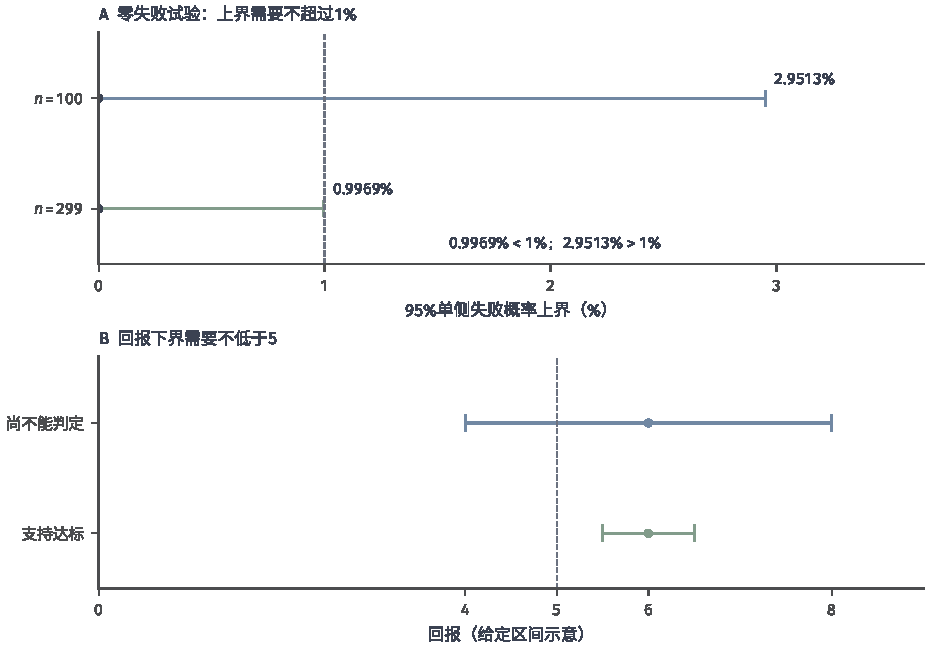
\includegraphics[width=157.400mm]{figures/10-reinforcement-learning/03-task-expansion-and-trustworthiness/matplotlib/rl-trustworthy-intervals.pdf}
  \caption{置信界与阈值的方向。上图按$n$次零失败的解析公式计算95\%单侧上界；下图仅以给定区间示意回报判断，不代表某个统计估计器或实验。点标估计，线段标可支持的指标范围。}
  \label{fig:rl-trustworthy-intervals}
\end{figure*}

达标判断还须绑定策略和协议版本。摩擦范围改变会影响轨迹分布，策略更新会影响状态动作占用，保护器升级会改变执行行为，参与者增加会改变闭环假设。旧运行记录未必全部失效，但须逐项说明哪些条件仍匹配、哪些运行记录需要重加权或补充、哪些模型性质须重新证明。交付对象或运行范围不再匹配时，旧安全声明不能直接沿用。

持续运行时，监测应检查保证前提：误差是否越出集合、备份是否仍可行、事件记录是否完整、干预比例是否明显改变。变化可触发保护、回退、收窄范围或补充取证，监测基础设施由系统卷讨论。统计判断也要覆盖查看方式：反复查看固定样本区间直到首次达标，并不自动保留原错误率。可预先为多次检验分配错误预算，或在相应评价记录的抽样条件下使用\term{置信序列}（confidence sequence），即对整个查看时间序列同时有效的界\scite{rl8-howard2021-sequences}

% Outline: 8.6
\section{多种要求的组合与取舍}
\label{sec:rl-trustworthy-combination}

三类要求至此分别讲完。为避免在不同任务上比较而让“任务本身的差异”掩盖“准则的差异”，现在把三类要求用于同一个导航选择。将基准网格抽象成单步路线选项任务：初态固定为起点，动作一次选择整段路线，结果给出到达终点总用时$T$、碰撞标记$I$和成本$C=10I$。这是独立教学模型，不使用基准网格的0.8滑移核；取$H=1$、不折扣、回报$G=-T$和损失$L=T$。路线内部的执行与恢复汇总为一次结果，时间以教学单位计。

候选集合先限定为四条确定路线A、B、C、D，所有比较固定同一初态和这组候选。干燥环境下，A以0.95概率用时5、以0.05概率用时25，B、C、D分别固定用时7、8、9。湿滑环境只将A、B用时各增加10，C、D不变。允许环境集合在本例中由这两个教学情形枚举给定，不是从观测记录估计的置信集。

两种环境中的碰撞概率依次为0.02、0.005、0.003、0。为分离时间与安全成本的影响，规定$I$和$T$独立，碰撞也不另外终止路线选项。这些假设共同确定联合分布，仅服务于控制变量比较，不是关于真实机器人碰撞与恢复的经验规律。

表~\ref{tab:rl-trustworthy-comparison}~据该联合分布精确计算。例如A平均用时为
$0.95\times5+0.05\times25=6$，0.95分位水平的CVaR为25，期望成本为$10\times0.02=0.2$，其余行用同样公式计算。回报越大越好，用时尾部、碰撞概率和成本越小越好。全部路线都关闭外部保护，干预为0；这只是固定执行机制，不是安全达标的证据。

\begin{table*}[t]
  \centering
  \begin{tabularx}{\linewidth}{@{}>{\raggedright\arraybackslash}p{14mm}XXXXXXX@{}}
    \toprule
    路线 & 标称平均回报 & 标称尾部损失 & 湿滑平均回报 & 碰撞概率 & 期望成本 & 干预比例 & 证据强度 \\
    \midrule
    A：捷径 & $-6$ & $25$ & $-16$ & $0.02$ & $0.20$ & $0$ & 教学模型精确值 \\
    B：定时 & $-7$ & $7$ & $-17$ & $0.005$ & $0.05$ & $0$ & 教学模型精确值 \\
    C：抗滑 & $-8$ & $8$ & $-8$ & $0.003$ & $0.03$ & $0$ & 教学模型精确值 \\
    D：保守 & $-9$ & $9$ & $-9$ & $0$ & $0$ & $0$ & 教学模型精确值 \\
    \bottomrule
  \end{tabularx}
  \caption{同一候选集合的解析教学比较。尾部损失为$\operatorname{CVaR}_{0.95}(T)$；碰撞概率和成本在两环境下按假设相同。D的零概率仅属于该指定模型，所有行均无真实部署统计证据。}
  \label{tab:rl-trustworthy-comparison}
\end{table*}

只最大化标称平均回报，会选A，却留下25的最差5\%平均用时。改为最小化标称尾部损失，选B，但其平均回报从干燥时的$-7$降到湿滑时的$-17$，回报减少10，也就是平均用时增加10。若最大化干燥与湿滑中的最坏平均回报，则选C；若仍优化标称均值，只增加期望成本预算$b=0.01$，四个确定候选中只有D可行。同一策略跨环境的下降幅度，还须与变化后的绝对值一起看：C、D的平均回报都没有下降，但变化后分别为$-8$与$-9$；若要求平均用时不超过8.5，C满足而D不满足。反过来，只看湿滑回报也无法区分原来就慢与湿滑额外造成的延误。这里的比较仍固定初态、候选和用时单位，每次求解只改一类要求，并非四个依次执行的算法阶段。

允许策略类若扩大到出发前随机选路线，结论还会变化。以0.2概率选B、0.8概率选D，期望成本为$0.2\times0.05=0.01$，平均用时为$0.2\times7+0.8\times9=8.6$，优于确定选D的9。因此D的上述最优性只针对四个确定候选，与示例~\ref{ex:rl-trustworthy-randomization}~相符。一次运行仍会完整选择B或D，不会走一条“平均路线”，B回合的碰撞可能也仍存在。

上面每次只施加一类要求。当它们同时出现时，不能简单地先按一个准则选策略、再指望它碰巧满足其余要求，而要把“在满足其余要求的策略中优化主目标”写成一个带约束的优化问题。这些要求若同时存在，须先由物理范围、枚举场景或观测记录给出的覆盖界确定模型族$\mathcal M$，再确定允许策略类$\Pi$。可以在保证最坏回报不太低、最坏成本不太高的前提下，最小化最坏风险：
\begin{align}
  \min_{\pi\in\Pi}\quad&
      \sup_{M\in\mathcal M}\mathcal R_M(L^\pi), \nonumber\\
  \text{满足}\quad&
      \inf_{M\in\mathcal M}J_M(\pi)\geq j_{\min}, \nonumber\\
  &\sup_{M\in\mathcal M}J_{c_i,M}(\pi)\leq b_i
       \quad (i=1,\ldots,m_c).
  \label{eq:rl-trustworthy-combined-problem}
\end{align}
这里$\mathcal R_M$须事先选为静态或动态风险，$\Pi$须说明历史依赖和随机化范围。风险与成本越大越差，故对模型取上确界；回报越小越差，故取下确界。这使每项要求分别覆盖全部允许模型。在路线例中，$\mathcal M$可以就是干燥与湿滑两情形；没有场景概率时，不能对二者作概率平均，即使给出概率，平均达标仍可能由干燥时的收益抵消湿滑时的违反，不能代替逐模型约束。只对回报作鲁棒优化，不会自动使成本鲁棒；鲁棒成本达标也不保证任务收益足够。

图~\ref{fig:rl-trustworthy-intersection}~将各项阈值对应的允许策略画成集合，最终可行域是这些集合与$\Pi$的交集。固定目标和策略类后，增加约束只能保持或缩小可行域，不会使最优值自动改善。在四个确定路线中，同时要求标称CVaR不超过8、最坏平均用时不超过9、期望成本不超过0.01，就没有可行选项：C满足前两项而成本超标，D满足后两项而尾部用时为9。此时须扩大策略类、改变环境或协商阈值；求解器返回的最少违反方案仍未满足原要求。

\begin{figure}[htbp]
  \centering
  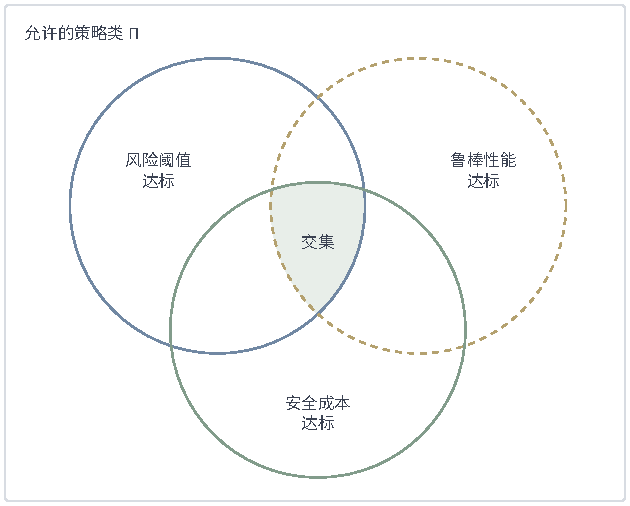
\includegraphics[width=106.652mm]{figures/10-reinforcement-learning/03-task-expansion-and-trustworthiness/tikz/rl-trustworthy-intersection.pdf}
  \caption{可行策略集合的概念示意，不是教学路线数值的几何嵌入。阴影为三种阈值共同允许的策略；在具体任务中，交集也可能为空。集合边界形状没有凸性含义。}
  \label{fig:rl-trustworthy-intersection}
\end{figure}

要识别保护器贡献，再固定同一候选，只切换保护是否启用。图~\ref{fig:rl-trustworthy-protected-path}~保留基准网格起终点和障碍，但采用无滑移的确定教学动力学，并将$(3,1)$规定为危险格。关闭保护，候选沿下方五步路径穿过危险格；启用保护，在$(2,1)$拒绝向右请求，转交已验证备份返回$(1,1)$，再沿上方到终点，共七步。该备份在这一确定模型中不进入障碍和危险格；恢复随机滑移后，须重新检查所有允许后继，原路径不能直接成为鲁棒安全证书。

\begin{figure}[htbp]
  \centering
  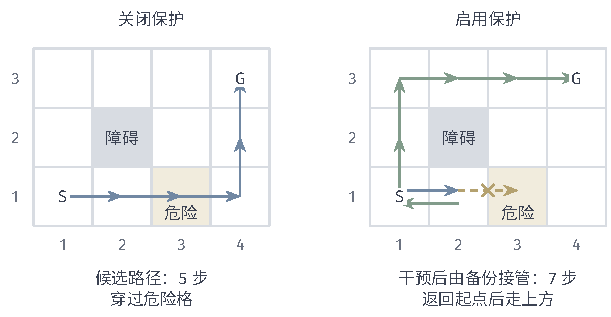
\includegraphics[width=103.470mm]{figures/10-reinforcement-learning/03-task-expansion-and-trustworthiness/tikz/rl-trustworthy-protected-path.pdf}
  \caption{同一候选启用或关闭保护的确定性路径示意，坐标、障碍和起终点沿用基准网格。虚线为被拒绝的请求，实线为实际路径；右图在干预后使用备份，不表示候选策略已自行学会绕行。}
  \label{fig:rl-trustworthy-protected-path}
\end{figure}

右图避免了一次危险格穿越，代价是两步额外行程和一次转入备份控制的切换。保持安全的是受保护系统，未保护候选仍请求经过危险格。图中一次拒绝也不等于全回合只替换一个动作，后续备份动作仍须由日志区分。保护改变了实际执行过程及其可见记录分布，学习器看到的安全轨迹可能来自外部修正；继续训练时须保留请求与实际动作，才能判断学到的是候选能力还是保护贡献。

这些比较同时呈现收益与代价。扩大不确定集合能增加覆盖范围，却可能降低可达到的回报；收紧尾部或安全阈值可能增加绕行与接管；加强保护能减少危险探索，却也会减少某些动作的观测，使其效果更难识别。因此方案结论需要同时声明行为标准、环境范围、执行机制与证据，单一平均分数不足以表达取舍。序贯决策的验证还须把其他已经明确的行为要求落实到实际策略、运行机制和评价记录，逐项规定可计算的指标、适用条件及证据。

% Outline: 8.7
\section{本章小结}
\label{sec:rl-trustworthy-summary}

导航例中，平均最快的路线未必尾部延误最小，尾部延误较小的路线未必耐受湿滑，耐受湿滑的路线又可能违反成本预算。风险准则比较随机后果，鲁棒要求覆盖允许环境，安全约束划定可行策略；三者可以组合，各自的评价目标、观测或环境模型要求及证明条件仍须分别保留。

\begin{table*}[htbp]
  \centering
  \begin{tabularx}{\linewidth}{@{}>{\raggedright\arraybackslash}p{22mm}XXX@{}}
    \toprule
    要求 & 决定性条件 & 方法 & 相应证据 \\
    \midrule
    控制累计尾部 & 损失、分位水平及事前承诺明确 & 静态CVaR采样更新、状态增广 & 尾部估计误差与留出轨迹 \\
    条件风险一致 & 条件映射及状态分量与递归目标匹配 & 嵌套风险Bellman更新 & 算子性质及条件风险估计 \\
    覆盖环境变化 & 扰动位置、扰动者可读字段与集合结构明确 & 鲁棒规划、受扰训练、状态估计 & 模型覆盖、内层误差与压力测试 \\
    平均成本达标 & 成本单位、初态、折扣及策略类明确 & 占用规划、原始--对偶与局部约束更新 & 最终策略的成本上界 \\
    事件概率达标 & 事件、时域、条件预算一致 & 事件采样、概率递推、预算分配 & 完整事件记录与有效概率上界 \\
    逐轨迹保持安全 & 误差范围有效、初态可行且保护输入存在 & 屏蔽、不变集、屏障与预测过滤 & 真实闭环符合证书全部前提 \\
    可靠地作出判断 & 交付对象、运行协议和取证程序固定 & 留出验证、联合置信与持续复核 & 界与阈值比较，并标明现有样本尚不足以判断达标 \\
    \bottomrule
  \end{tabularx}
  \caption{本章的要求、条件、方法与证据。算法的优化目标与交付时能够成立的保证是两件需要分别检查的事。}
  \label{tab:rl-trustworthy-summary}
\end{table*}

静态累计CVaR保留事前损失分布，嵌套风险逐层评价条件后果，状态增广与时间一致性要服务于对应目标。鲁棒备份须明确扰动作用于动力学、观测还是执行通道，并保存对手权限所需的状态；矩形性才使局部最坏选择组成合法模型。期望成本允许个别高成本轨迹，事件概率允许有限违约概率，硬要求则在声明范围内排除违约。乘子、概率预算和安全过滤据此维护不同性质。

表~\ref{tab:rl-trustworthy-summary}~对应每项要求的条件、方法与证据。方法的名称不足以判断可信性，还需确定它维护的性质、评价固定策略还是受保护系统、依赖哪些模型和记录采集前提，以及这些前提改变后哪些结论仍成立。



若日志支持不足或隐藏风险不可识别，需要回到第~\ref{chap:rl-information}~章的观测范围、日志字段与动作覆盖条件；若奖励没有表达真正意图，需要第~\ref{chap:rl-reward}~章的奖励分析。新任务识别与适应由第~\ref{chap:rl-transfer}~章讨论，其他参与者响应由第~\ref{chap:rl-multi-agent}~章提供模型。这些条件改变时，既要检查决策问题是否改变，也要复核原证据是否仍覆盖交付对象；求解结束本身并不构成可信性保证。

